% uWaterloo Thesis Template for LaTeX 
% Last Updated Nov 4, 2016 by Stephen Carr, IST Client Services
% FOR ASSISTANCE, please send mail to rt-IST-CSmathsci@ist.uwaterloo.ca

% Effective October 2006, the University of Waterloo 
% requires electronic thesis submission. See the uWaterloo thesis regulations at
% https://uwaterloo.ca/graduate-studies/thesis.

% DON'T FORGET TO ADD YOUR OWN NAME AND TITLE in the "hyperref" package
% configuration below. THIS INFORMATION GETS EMBEDDED IN THE PDF FINAL PDF DOCUMENT.
% You can view the information if you view Properties of the PDF document.

% Many faculties/departments also require one or more printed
% copies. This template attempts to satisfy both types of output. 
% It is based on the standard "book" document class which provides all necessary 
% sectioning structures and allows multi-part theses.

% DISCLAIMER
% To the best of our knowledge, this template satisfies the current uWaterloo requirements.
% However, it is your responsibility to assure that you have met all 
% requirements of the University and your particular department.
% Many thanks for the feedback from many graduates that assisted the development of this template.

% -----------------------------------------------------------------------

% By default, output is produced that is geared toward generating a PDF 
% version optimized for viewing on an electronic display, including 
% hyperlinks within the PDF.
 
% E.g. to process a thesis called "mythesis.tex" based on this template, run:

% pdflatex mythesis	-- first pass of the pdflatex processor
% bibtex mythesis	-- generates bibliography from .bib data file(s)
% makeindex         -- should be run only if an index is used 
% pdflatex mythesis	-- fixes numbering in cross-references, bibliographic references, glossaries, index, etc.
% pdflatex mythesis	-- fixes numbering in cross-references, bibliographic references, glossaries, index, etc.

% If you use the recommended LaTeX editor, Texmaker, you would open the mythesis.tex
% file, then click the PDFLaTeX button. Then run BibTeX (under the Tools menu).
% Then click the PDFLaTeX button two more times. If you have an index as well,
% you'll need to run MakeIndex from the Tools menu as well, before running pdflatex
% the last two times.

% N.B. The "pdftex" program allows graphics in the following formats to be
% included with the "\includegraphics" command: PNG, PDF, JPEG, TIFF
% Tip 1: Generate your figures and photos in the size you want them to appear
% in your thesis, rather than scaling them with \includegraphics options.
% Tip 2: Any drawings you do should be in scalable vector graphic formats:
% SVG, PNG, WMF, EPS and then converted to PNG or PDF, so they are scalable in
% the final PDF as well.
% Tip 3: Photographs should be cropped and compressed so as not to be too large.

% To create a PDF output that is optimized for double-sided printing: 
%
% 1) comment-out the \documentclass statement in the preamble below, and
% un-comment the second \documentclass line.
%
% 2) change the value assigned below to the boolean variable
% "PrintVersion" from "false" to "true".

% --------------------- Start of Document Preamble -----------------------

% Specify the document class, default style attributes, and page dimensions
% For hyperlinked PDF, suitable for viewing on a computer, use this:
\documentclass[letterpaper,12pt,titlepage,oneside,final]{book}
 
% For PDF, suitable for double-sided printing, change the PrintVersion variable below
% to "true" and use this \documentclass line instead of the one above:
%\documentclass[letterpaper,12pt,titlepage,openright,twoside,final]{book}

% Some LaTeX commands I define for my own nomenclature.
% If you have to, it's better to change nomenclature once here than in a 
% million places throughout your thesis!
\newcommand{\package}[1]{\textbf{#1}} % package names in bold text
\newcommand{\cmmd}[1]{\textbackslash\texttt{#1}} % command name in tt font 
\newcommand{\href}[1]{#1} % does nothing, but defines the command so the
    % print-optimized version will ignore \href tags (redefined by hyperref pkg).
%\newcommand{\texorpdfstring}[2]{#1} % does nothing, but defines the command
% Anything defined here may be redefined by packages added below...

% This package allows if-then-else control structures.
\usepackage{ifthen}
\newboolean{PrintVersion}
\setboolean{PrintVersion}{false} 

\usepackage{threeparttable}
\usepackage{epigraph}
\usepackage{csquotes}
\usepackage{xr}
\usepackage[hang,flushmargin]{footmisc} 
% CHANGE THIS VALUE TO "true" as necessary, to improve printed results for hard copies
% by overriding some options of the hyperref package below.

%\usepackage{nomencl} % For a nomenclature (optional; available from ctan.org)
\usepackage{amsmath,amssymb,amstext} % Lots of math symbols and environments
\usepackage[pdftex]{graphicx} % For including graphics N.B. pdftex graphics driver 

% Hyperlinks make it very easy to navigate an electronic document.
% In addition, this is where you should specify the thesis title
% and author as they appear in the properties of the PDF document.
% Use the "hyperref" package 
% N.B. HYPERREF MUST BE THE LAST PACKAGE LOADED; ADD ADDITIONAL PKGS ABOVE
\usepackage[pdftex,pagebackref=false]{hyperref} % with basic options
		% N.B. pagebackref=true provides links back from the References to the body text. This can cause trouble for printing.
\hypersetup{
    plainpages=false,       % needed if Roman numbers in frontpages
    unicode=false,          % non-Latin characters in Acrobat’s bookmarks
    pdftoolbar=true,        % show Acrobat’s toolbar?
    pdfmenubar=true,        % show Acrobat’s menu?
    pdffitwindow=false,     % window fit to page when opened
    pdfstartview={FitH},    % fits the width of the page to the window
    pdftitle={uWaterloo\ LaTeX\ Thesis\ Template},    % title: CHANGE THIS TEXT!
%    pdfauthor={Author},    % author: CHANGE THIS TEXT! and uncomment this line
%    pdfsubject={Subject},  % subject: CHANGE THIS TEXT! and uncomment this line
%    pdfkeywords={keyword1} {key2} {key3}, % list of keywords, and uncomment this line if desired
    pdfnewwindow=true,      % links in new window
    colorlinks=true,        % false: boxed links; true: colored links
    linkcolor=blue,         % color of internal links
    citecolor=green,        % color of links to bibliography
    filecolor=magenta,      % color of file links
    urlcolor=cyan           % color of external links
}
\ifthenelse{\boolean{PrintVersion}}{   % for improved print quality, change some hyperref options
\hypersetup{	% override some previously defined hyperref options
%    colorlinks,%
    citecolor=black,%
    filecolor=black,%
    linkcolor=black,%
    urlcolor=black}
}{} % end of ifthenelse (no else)
\usepackage{enumitem}
\usepackage[natbibapa]{apacite}
\usepackage[automake,toc,abbreviations]{glossaries-extra} % Exception to the rule of hyperref being the last add-on package

% Setting up the page margins...
% uWaterloo thesis requirements specify a minimum of 1 inch (72pt) margin at the
% top, bottom, and outside page edges and a 1.125 in. (81pt) gutter
% margin (on binding side). While this is not an issue for electronic
% viewing, a PDF may be printed, and so we have the same page layout for
% both printed and electronic versions, we leave the gutter margin in.
% Set margins to minimum permitted by uWaterloo thesis regulations:
\setlength{\marginparwidth}{0pt} % width of margin notes
% N.B. If margin notes are used, you must adjust \textwidth, \marginparwidth
% and \marginparsep so that the space left between the margin notes and page
% edge is less than 15 mm (0.6 in.)
\setlength{\marginparsep}{0pt} % width of space between body text and margin notes
\setlength{\evensidemargin}{0.125in} % Adds 1/8 in. to binding side of all 
% even-numbered pages when the "twoside" printing option is selected
\setlength{\oddsidemargin}{0.125in} % Adds 1/8 in. to the left of all pages
% when "oneside" printing is selected, and to the left of all odd-numbered
% pages when "twoside" printing is selected
\setlength{\textwidth}{6.375in} % assuming US letter paper (8.5 in. x 11 in.) and 
% side margins as above
\raggedbottom

% The following statement specifies the amount of space between
% paragraphs. Other reasonable specifications are \bigskipamount and \smallskipamount.
\setlength{\parskip}{\medskipamount}

% The following statement controls the line spacing.  The default
% spacing corresponds to good typographic conventions and only slight
% changes (e.g., perhaps "1.2"), if any, should be made.
\renewcommand{\baselinestretch}{1} % this is the default line space setting

% By default, each chapter will start on a recto (right-hand side)
% page.  We also force each section of the front pages to start on 
% a recto page by inserting \cleardoublepage commands.
% In many cases, this will require that the verso page be
% blank and, while it should be counted, a page number should not be
% printed.  The following statements ensure a page number is not
% printed on an otherwise blank verso page.
\let\origdoublepage\cleardoublepage
\newcommand{\clearemptydoublepage}{%
  \clearpage{\pagestyle{empty}\origdoublepage}}
\let\cleardoublepage\clearemptydoublepage

\makeglossaries

%======================================================================
%   L O G I C A L    D O C U M E N T -- the content of your thesis
%======================================================================
\begin{document}

% For a large document, it is a good idea to divide your thesis
% into several files, each one containing one chapter.
% To illustrate this idea, the "front pages" (i.e., title page,
% declaration, borrowers' page, abstract, acknowledgements,
% dedication, table of contents, list of tables, list of figures,
% nomenclature) are contained within the file "uw-ethesis-frontpgs.tex" which is
% included into the document by the following statement.
%----------------------------------------------------------------------
% FRONT MATERIAL
%----------------------------------------------------------------------
% T I T L E   P A G E
% -------------------
% Last updated Nov 1, 2016, by Stephen Carr, IST-Client Services
% The title page is counted as page `i' but we need to suppress the
% page number.  We also don't want any headers or footers.
\pagestyle{empty}
\pagenumbering{roman}

% The contents of the title page are specified in the "titlepage"
% environment.
\begin{titlepage}
        \begin{center}
        \vspace*{1.0cm}

        \Huge
        {\bf Inferential Role Semantics for Natural Language}

        \vspace*{1.0cm}

        \normalsize
        by \\

        \vspace*{1.0cm}

        \Large
        Peter Blouw \\

        \vspace*{3.0cm}

        \normalsize
        A thesis \\
        presented to the University of Waterloo \\ 
        in fulfillment of the \\
        thesis requirement for the degree of \\
        Doctor of Philosophy \\
        in \\
        Philosophy \\

        \vspace*{2.0cm}

        Waterloo, Ontario, Canada, 2017 \\

        \vspace*{1.0cm}

        \copyright\ Peter Blouw 2017 \\
        \end{center}
\end{titlepage}

% The rest of the front pages should contain no headers and be numbered using Roman numerals starting with `ii'
\pagestyle{plain}
\setcounter{page}{2}

\cleardoublepage % Ends the current page and causes all figures and tables that have so far appeared in the input to be printed.
% In a two-sided printing style, it also makes the next page a right-hand (odd-numbered) page, producing a blank page if necessary.
 


% D E C L A R A T I O N   P A G E
% -------------------------------
  % The following is a sample Delaration Page as provided by the GSO
  % December 13th, 2006.  It is designed for an electronic thesis.
  \noindent
I hereby declare that I am the sole author of this thesis. This is a true copy of the thesis, including any required final revisions, as accepted by my examiners.

  \bigskip
  
  \noindent
I understand that my thesis may be made electronically available to the public.

\cleardoublepage

% A B S T R A C T
% ---------------

\begin{center}\textbf{Abstract}\end{center}

The most general goal of semantic theory is to explain facts about language use. In keeping with this goal, I introduce a framework for thinking about linguistic expressions in terms of (a) the inferences they license, (b) the behavioral predictions that their uses thereby sustain, and (c) the affordances that they provide to language users in virtue of these inferential and predictive involvements. Within my framework, linguistic expressions acquire meanings by regulating social practices that involve ``intentional interpretation,'' wherein people explain and predict one another's behavior through linguistically specified mental state attributions. Developing a theory of meaning therefore requires formalizing the inferential roles that determine how linguistic expressions regulate intentional interpretation. Accordingly, the view I develop is an inferential role semantics for natural language.

To describe this semantics, I take advantage of recently developed techniques in the field of natural language processing. I introduce a model that assigns inferential roles to arbitrary linguistic expressions by learning from examples of how sentences are distributed as premises and conclusions in a space of possible inferences. I then empirically evaluate the model's ability to generate accurate entailments for novel sentences not used as training examples. I argue that this model takes a small but important step towards codifying the meanings of the expressions it manipulates.

Next, I examine the theoretical implications of this work with respect to debates about the compositionality of language, the relationship between language and cognition, and the relationship between language and the world. With respect to compositionality, I argue that the debate is really about generalization in language use, and that the required sort of generalization can be achieved by ``interpolating'' between familiar examples of correct inferential transitions. With respect to the relationship between thought and language, I argue that it is a mistake to try to derive a theory of natural language semantics from a prior theory of mental representation because theories of mental representation invoke the sort of intentional interpretation at play in language use from the get-go. With respect to the relationship between language and the world, I argue that questions about truth conditions and reference relations are best thought of as questions about the normative statuses of linguistic acts. These normative statuses, in turn, are best defined in primarily inferential terms. 

I conclude with an all-things-considered evaluation of my theory that demonstrates how it overcomes a number of challenges associated with semantic theories that take inference, rather than reference, as their starting point. 


\cleardoublepage

% A C K N O W L E D G E M E N T S
% -------------------------------

\begin{center}\textbf{Acknowledgements}\end{center}

TBD - Thanks to all who helped.
\cleardoublepage

% T A B L E   O F   C O N T E N T S
% ---------------------------------
\renewcommand\contentsname{Table of Contents}
\tableofcontents
\cleardoublepage
\phantomsection    % allows hyperref to link to the correct page

% L I S T   O F   T A B L E S
% ---------------------------
\addcontentsline{toc}{chapter}{List of Tables}
\listoftables
\cleardoublepage
\phantomsection		% allows hyperref to link to the correct page

% L I S T   O F   F I G U R E S
% -----------------------------
\addcontentsline{toc}{chapter}{List of Figures}
\listoffigures
\cleardoublepage
\phantomsection		% allows hyperref to link to the correct page

% Change page numbering back to Arabic numerals
\pagenumbering{arabic}

 

%----------------------------------------------------------------------
% MAIN BODY
%----------------------------------------------------------------------
% Because this is a short document, and to reduce the number of files
% needed for this template, the chapters are not separate
% documents as suggested above, but you get the idea. If they were
% separate documents, they would each start with the \chapter command, i.e, 
% do not contain \documentclass or \begin{document} and \end{document} commands.
%======================================================================
%----------------------------------------------------------------------
% MAIN BODY
%----------------------------------------------------------------------

%======================================================================
\chapter{What Meanings Do}
%======================================================================
\renewcommand{\epigraphrule}{0pt}
\setlength{\epigraphwidth}{4.5in}
\epigraph{\textit{In order to say what a meaning is, we may first ask what a meaning does, and then find something that does that.}}{- David Lewis, 1970}

\setlength{\epigraphwidth}{4.5in}
\epigraph{\textit{The point of the theoretical association of meanings with linguistic expressions is to explain the use of those expressions.}}{- Robert Brandom, 2000}

\section{Introduction}

While it is quite clear that Lewis' methodological advice has played a central role in the development of contemporary semantics \citep{LiangPotts:2015}, it is less clear that any consensus has arisen regarding its appropriate application. Common sense suggests that meanings do the job of lending communicative significance to sounds and scribbles that would otherwise be of little interest to us, yet researchers have seen fit to assign a rather diverse set of responsibilities to semantic theory. 

On the one hand, meanings have been invoked to explain how language connects to reality via relations of reference, and to thereby explain how certain configurations of reality are compatible with the truth of some sentences but not others \citep{Speaks:2014,Lewis:1970,Soames:2010}. On the other hand, meanings have also been invoked to explain various facts about language use \citep{Wittgenstein:1953,Brandom:1994,Brandom:2000,Horwich:2005,Horwich:1998} and the psychological states of language users \citep{Block:1986,Harman:1982}. Given these diverse aims, one can legitimately wonder whether the various theories of meaning that have been proposed are really theories of the same sort \citep{Block:1986}. And even if they are of the same sort, one can go on to wonder whether it is possible for a single theory to satisfy all of the aims in question \citep{Horwich:1998}. 

My goal in this thesis is to argue that ``meanings'' function mainly to codify our implicit expectations regarding certain effects of language use. This idea fits comfortably into a long tradition of work characterizing meaning in terms of use \citep{Sellars:1954,Wittgenstein:1953,Sellars:1953,Harman:1982,Block:1986,Brandom:1994,Brandom:2000,Brandom:2009,Horwich:2005}, but as I hope to show, it provides novel resources for avoiding some of the pitfalls to be found in this earlier work. Specifically, I argue that linguistic expressions can be thought of as informal instruments of prediction that are used in social practices involving ``intentional interpretation'' \citep{Dennett:1987,Brandom:1994}.\footnote{Intentional interpretation (i.e., the adoption of Dennett's (\citeyear{Dennett:1987,Dennett:1991}) ``intentional stance'') is the practice of explaining or predicting an agent’s behavior via the use of mental state attributions.} When others use particular words and sentences, it allows us to predict what they are likely to do and say next; when we use particular words and sentences, it allows us to have predictable effects on others. The goal of semantic theory, considered as a scientific enterprise, is accordingly to account for how language is able to perform this predictive function in the context of intentional interpretation. The key to developing such a theory, on my view, is to formalize the tacit inferential relationships that hold amongst various linguistic expressions and non-linguistic perceptions and actions, and thus explain how tacit expectations are generated on the basis of these relationships. I accordingly propose an inferential role semantics for natural language in what follows. 

To develop this semantics in more detail, I introduce what I refer to as the IPA framework for theorizing about language use. The framework uses notions of inference (I), prediction (P), and affordance (A) to build on the commonplace observation that language use is a species of joint action (akin to a dance) in which two or more people co-ordinate their behavior so as to engage in successful communication \citep{Clark:1996,Brandom:2010a}. In order for such co-ordination to occur, language users need to understand the effects that their linguistic acts will have on how a conversation unfolds, in much the same way that dancers need to understand the effects that their movements will have on how a dance unfolds. In the case of a dance, the principle effect of making a particular movement (e.g., a forward step) is to license one's partner to make an appropriate movement in response (e.g., a backward step). In the case of a conversation, the principle effect of uttering a sentence is to license others to draw certain inferences. For instance, if one person states that they go sailing frequently, then it licenses others to infer that they spent time on the water and have experience with strong winds, amongst many other things. An important function of such inferential relations is to ``lead'' the conversation in a particular direction by making it appropriate for others to ask certain questions (e.g., ``Do you ever get seasick?'') and make certain statements (e.g., ``I personally prefer the speed of motorboats''). If it is further assumed that conversationalists are rational and cooperative, then the inferential relations in question can be used to generate predictions about how the conversation will likely unfold, in much the same way that certain relationships amongst dance movements can be used to generate predictions about how a dance will likely unfold. Finally, the fact that linguistic acts license certain inferences and sustain certain predictions means that they afford certain opportunities to manipulate the trajectory of a conversation. One can, in other words, steer a conversation with a particular utterance, in much the same way that one can steer a dance with a particular movement.\footnote{As a further application of the analogy, notice that dances and conversations are similarly varied with respect to their formality, purpose, duration, and underlying conventions.}

Overall, the three components of the IPA framework can be summarized as follows: the inferences licensed by a particular linguistic expression determine what effect an utterance of the expression \textit{ought} to have on the conversation; one can thereby predict what effect the utterance likely \textit{will} have on a conversation with a rational and cooperative partner; and given that the utterance ought to and will likely have these effects, the expression in question makes it such that individuals \textit{can} have these effects on a conversation, if doing so is in accordance with their goals. The purpose of the IPA framework is accordingly to elaborate on the idea that language users engage in intentional interpretation in order to anticipate and control the trajectory of a conversation.

Three informal observations can help to give the IPA framework some initial plausibility. First, the fact that competent speakers are unable to catalog the meanings of the expressions in their language provides \textit{prima facie} evidence that knowledge of meaning is not knowledge of explicit fact. When competent language users invoke morphological variants of the verb ``to mean,'' they often do so to to correct or instruct someone regarding the proper usage of a term of interest. For instance, utterances of the following sort are quite familiar: ``That's not what \textit{versatile} means - something is versatile if it can be put to use in a variety of ways.'' On the other hand, utterances of the form ``the meaning of \textit{X} is \textit{Y},'' where \textit{X} is a natural language expression and \textit{Y} is a meaning, are patently unfamiliar. As such, there is good reason to suppose that understanding a meaning involves implicitly understanding how to use a linguistic expression \citep{Brandom:1994,Horwich:2005}.

Second, it is quite clear that we form expectations about what other people are likely to do based on what \textit{we} tell them and what \textit{they} tell us. For example, if you tell me that you dislike chocolate, I can reasonably expect you to avoid ordering chocolate cake for dessert. Similarly, if I tell you that I own a dog, then I can reasonably expect you to respond affirmatively if someone else asks you whether I own any pets. These predictions are importantly dependent on the particular expressions present in each utterance. If the word ``chocolate'' is replaced with the compound word ``ice cream'' in the first example, then a new set of expectations are in order -- it would no longer be prudent for me to expect that you will avoid chocolate desserts. The point here is that in the absence of minimally correct predictions about what follows from the use of a particular expression, it is implausible to presume an understanding of what the expression means. Overall, language use is fraught with expectations on the part of language users.
 
Third, the existence of these expectations has obvious instrumental value in social contexts. The ability to make successful predictions concerning the state of the world is a prerequisite for survival in most living creatures \citep{clark:2013,Dennett:1987}, and when the state of the world is partly constituted by other living creatures, it is useful to be well informed about what these other creatures are going to do. A language can accordingly be thought of as a social technology that sustains a shared measure of predictive success in the context of collective activity. Put simply, people learn more than they would otherwise learn about what to expect from the world by talking to one another.\footnote{Two misunderstandings are worth defending against on this point. First, debates about how language evolved are immaterial in this context; what matters is that it did evolve, and that it possesses properties that help sustain complex forms of cooperative activity. Second, no stand is being taken regarding the conditions that need to be met in order for something to count as a language. The growls one wolf makes towards another wolf can be thought of as a primitive form of linguistic activity, since growls can facilitate expectations (e.g., the second wolf can expect a potential attack from the first) that help sustain collective activity (e.g., the behavior of a wolf pack). Though it is clear that human language is importantly different from these more primitive forms of communication \citep{Pinker:1994,Harley:2014}} It is also worth highlighting how analogous these social predictions are to the kinds of physical predictions that are afforded so naturally by observation. People, for instance, generally expect that an object will fall if nothing is present to hold it up, and that materials of particular types can manipulated in particular ways \citep{Dennett:1987}. Similarly, people also expect that various uses of language have predictable effects on the thoughts and behaviors of others. For example, if one asks the question ``What are car seats made of?'', being given the response ``It's warm outside today'' is almost as surprising as seeing a vase remain upright after being tilted forty-five degrees. A natural extension of these comparisons is the idea that a theory of meaning accounts for certain linguistic phenomena in approximately the same way that a physical theory account for physical phenomena. The goals of theory development in each case include explaining \textit{why} things like tilted vases and verbal non-sequiturs are so surprising. 

On the basis of these informal observations, I think it is reasonable to seriously consider treating meanings as posits of a theory that aims to explain how and why people use linguistic expressions in the ways that they do. Attributing a meaning to sentence is not unlike attributing a center of mass to an object or charge to a particle \citep[see][]{Dennett:1987}; in all such cases, the attribution is warranted because it lends explanatory insight into certain phenomena of interest (i.e., phenomena involving sentences, objects, and particles respectively). To lend further support to these claims, I will largely adopt a demonstrative strategy. That is, I will initially assume that meanings ought to be treated this way, and then go on to demonstrate various kinds of valuable explanatory work that can be done given the assumption. Over the course of these demonstrations, I will also clearly identify various aspects of linguistic analysis that do not involve meanings directly. For instance, syntax (the study of phrase and sentence structure), morphology (the study of word structure), and phonology (the study of sound structure) all have a role to play in explaining linguistic phenomena, but they do not by this measure count as semantic. Similarly, the study of certain pragmatic features of language use also falls outside of the domain of semantics. For example, it is reasonable to expect that questions are followed by answers over the course of a dialogue, but this expectation is about conversational norms and not about the meaning of any particular linguistic expression.

The rest of this chapter is divided into four sections. First, I outline a set of theoretical criteria that follow from my characterization of the explanatory goals of semantic theory. Second, I provide a critical analysis of how existing approaches to semantics measure up against these criteria. Third, I provide a number of arguments in favor of the inferential role semantics that falls out of the IPA framework. The basic idea, again, is that linguistic expressions mean what they do in virtue of the inferences and predictions they license in the context of social practices that involve intentional interpretation (i.e., practices that involve people attributing mental states to one another). The view is accordingly similar in spirit to the work of Dennett (\citeyear{Dennett:1987,Dennett:1991}) and Brandom (\citeyear{Brandom:1994,Brandom:2009,Brandom:2000}). Finally, I conclude with a discussion of open problems and potential objections that are addressed throughout the remainder of the thesis. 

\section{Criteria for a Theory of Meaning}

Given the methodological assumption that meaning attributions should explain facts about language use, I propose a set of five criteria for evaluating competing semantic theories. The criteria are:

\begin{enumerate}
  \item Predictive adequacy
  \item Cognitive plausibility
  \item Compositionality
  \item Intentionality
  \item Normativity
\end{enumerate}

\noindent
While these criteria are somewhat distinct from those commonly found in the literature, they should not be entirely surprising. One job of semantics is to provide an account of our shared expectations concerning certain consequences of linguistic activity, but it is quite clear that these consequences are neither simple nor homogeneous. They can involve the mental states and surroundings of language users, and they are as innumerable as the linguistic expressions from which they arise. Moreover, they are the sort of thing that speakers can be mistaken about. The criteria are intended to reflect that the consequences of linguistic activity can be analyzed along these various dimensions. A few comments about each criterion are accordingly in order.

The predictive adequacy criterion is meant to capture the idea that the attribution of a particular meaning to a linguistic expression is warranted only when doing so has explanatory value \citep[see][for related ideas]{Hochstein:2011,Dennett:1987}. Such value, I contend, arises when the meaning attributed to a particular expression gives rise to successful predictions concerning (a) the cognitive states of individuals who use the expression, and (b) the behavior of such individuals. To illustrate with an example, consider the following sentence: ``The boy waited for the pitch and then hit the ball over the fence.'' A competent speaker of English is able to rapidly infer on the basis of this sentence that the boy is likely playing baseball, that he has likely used a bat to hit the ball, and that the phrase ``over the fence'' describes where the ball went after he hit it, rather than the location of the ball when he hit it. The predictive adequacy criterion favours attributing a meaning to this sentence that accounts for the fact that anyone who correctly understands it will provide appropriate answers to questions such as ``Where did the ball go?'' or ``What did the boy likely use to hit the ball?'' Finally, it is worth emphasizing that these expectations are most naturally understood in probabilistic rather than deductive terms: a meaning attribution does not entail the truth of certain counterfactual conditionals concerning linguistic or cognitive phenomena; rather, it favours such conditionals in a violable manner.

The cognitive plausibility criterion is motivated by the idea that if meanings are the sorts of things that are \textit{understood} by language users, then facts about meanings must be consistent with facts about language users' cognitive capacities. An example of a relevant fact about these cognitive capacities is the existence of a memory bottleneck that requires the brain to rapidly compress and recode linguistic input; otherwise, the current input is overwritten by new inputs and lost forever \citep{Christiansen:2015}. If a theory of semantics requires that language users retain highly detailed memories of the linguistic stimuli they encounter, then the theory runs afoul of a well-established result of psycholinguistic research. However, such research can also suggest new hypotheses about the nature of the expectations people form on the basis linguistic activity. For instance, the existence of a memory bottleneck suggests that these expectations are unlikely to be so fine-grained as to indicate the exact word transitions or motor behaviors exhibited by another person. The overall point here is that the cognitive plausibility criterion favours the co-development of theories of cognition and language use that are consistent with one another. An obvious example of this kind of co-development can be found in philosophical work that describes the meaning of a sentence in terms of the proposition it expresses, and describes the mental state of a person who understands the sentence in terms of their attitude towards the proposition in question \citep[][Ch. 5]{Dennett:1987}. Whether propositional theories of this sort are successful is, of course, another matter.

The compositionality criterion is motivated by the fact that people are able to understand and produce indefinitely large numbers of linguistic expressions. Many researchers believe that the only way to explain this fact is to suppose that the meanings of complex linguistic expressions are built up from the meanings of simple expressions through the recursive application of a fixed set of syntactic rules \citep{Szabo:2012,Szabo:2013,FodorLepore:1991,Recanati:2012,Unnsteinsson:2014,Pinker:1994,FodorPylyshyn:1988,CappelenLepore:2005}. If meanings were not compositional, it would be difficult to explain how people are able to learn infinitely productive languages from finite amounts of linguistic data. However, it is important to note that the compositionality criterion does not strictly enforce rule-based accounts of the relations between simple and complex meanings. Any non-rule-based account that has the capacity to account for the learnability and use of an infinitely productive language counts as compositional on my view. To illustrate this point, it is worth noting that many non-verbal creatures appear to possess infinitely productive capacities to exploit their physical environments, since these environments can contain indefinitely large numbers of distinct configurations of features. Yet few would argue that non-verbal creatures make use of a system of rules analogous to those proffered by linguists to guide their behavior \citep[cf.][]{FodorPylyshyn:1988}. As such, the compositionality criterion is about whether a theory has sufficient scope to account for the vast number of distinct linguistic expressions, and not about the precise shape the theory takes.\footnote{It might be better to call it a ``generality'' criterion, but I have opted to stick with conventional terminology so as to orient the discussion in a familiar way.}

The intentionality criterion concerns the idea that linguistic expressions are \textit{about} things and therefore bear important relations to non-linguistic entities such as objects, events, and properties \citep{Speaks:2014,Stanley:2008}. This criterion is accepted by many theorists on essentially stipulative grounds: what makes a linguistic expression meaningful is precisely the fact that it can represent or stand in for something else. Satisfying the intentionality criterion requires giving an account of the facts that determine exactly which things a given linguistic expression is about \citep{Horwich:1998,Brandom:2000}. Unfortunately, philosophers have developed many accounts of this sort in recent decades, none of which are without serious problems \citep{Horwich:2005}. In subsequent portions of this thesis, I will use the seemingly intractable nature of these problems to motivate an approach on which the ``aboutness'' of linguistic expressions is characterized in terms of the norms that govern language use. For the time being, however, the intentionality criterion can be sufficiently well motivated by noting that if linguistic expressions were to fail to be about things, it would be difficult to make sense of some very obvious features of communication. To give an example, the sentence ``The saucepan is boiling'' means what it does at least in part because it communicates information \textit{about} a particular saucepan. To give a slightly different example, the phrase ``kick the bucket'' is atypical and idiomatic precisely because it does \textit{not} convey information about a bucket.
 
The normativity criterion, finally, is motivated by the observation that uses of language are subject to evaluations of correctness \citep{Wittgenstein:1953,Brandom:1994,Brandom:2000,Brandom:2009,Sellars:1954,Kripke:1982}. To give a simple example, describing a sea otter as a type of fish constitutes a misuse of the term ``fish.'' Similarly, stating that ``Waterloo is to the east of Toronto'' on the basis of the fact that ``Waterloo is to the west of Toronto'' constitutes a violation of the norms governing uses of the words ``east'' and ``west'' \citep[i.e., they are not synonyms; see][p. 98]{Brandom:1994}. Specifying the nature of these norms, however, is a complicated matter \citep{Brandom:1994,Kripke:1982}. On one view, they emerge from the interactions between members of a linguistic community, and are irreducible to non-normative facts about this community \citep{Brandom:1994}. On another view, norms emerge from the demands of instrumental rationality \citep{Horwich:1998}, which can in turn be explained in terms of evolutionary pressures that have shaped us into the kinds of creatures that we are \citep{Dennett:1987,Dennett:2010}. Regardless of whether either of these views is correct, it is hard to dispute that what an expression means determines how one \textit{ought} to use it; the very fact that meanings are learned (and hence can be learned in error) presupposes as much. As such, a theory of semantics must have something to say about the fact that there are correct and incorrect uses of linguistic expressions.

One interesting feature of these criteria is that they can be construed as more or less general ways of imposing the requirement of predictive adequacy on a theory of meaning. To explain, the cognitive plausibility criterion can be thought of as ruling out theories that are predictively \textit{inadequate} when it comes to characterizing the obvious connections between language and cognition. The compositionality criterion similarly rules out theories that fail to generate good predictions concerning phenomena involving all of the indefinitely large number of possible expressions in a given language. The intentionality criterion rules out theories that are predictively inadequate when it comes to characterizing connections between language use and various non-linguistic perceptions and actions that people employ to interact with the world. The normativity criterion, finally, can be thought of as ruling out theories that assign no degree of impropriety to completely unpredictable forms of linguistic activity. It should accordingly be clear why these criteria have been selected -- they are consistent with the aims of a theory of meaning that is both predictive and explanatory, and therefore fit to play a role in the scientific study of language.  

\section{A Brief History of Semantics}

The approach and the criteria that I have introduced are in many ways at odds with conventional wisdom in philosophy. For this reason, I briefly evaluate two dominant traditions in the study of meaning to illustrate where and why I think conventional wisdom goes awry. The first tradition uses the concepts of truth and reference to define the meanings of various linguistic expressions. These definitions are then used in tandem with certain ancillary hypotheses about social cooperation to derive explanations of various regularities in language use \citep[e.g.,][]{Soames:2010,Lewis:1970,Lewis:1975,Davidson:1967,CappelenLepore:2005,Grice:1975}. The second tradition reverses this order of explanation: first, meanings are analyzed in terms of various regularities and social norms that govern language use; then, this analysis is used to derive an explanation of how linguistic expressions take on truth-values and refer to things in the world \citep[e.g.,][]{Wittgenstein:1953,Brandom:1994,Brandom:2000,Horwich:2005}. Numerous variations on these two basic approaches that can be found in recent work on semantic context-sensitivity \citep{Recanati:2004,CappelenLepore:2005}, and on disputes about the boundary between semantics and pragmatics \citep{Brandom:2000,Recanati:2012}.\footnote{Semantics is typically characterized as the study of linguistic meaning, while pragmatics is typically characterized as the study of language use. Pragmatics is also sometimes characterized as the study of context-sensitivity in language, though this is arguably the same as the first definition, since shifts in context are what make different uses of the same linguistic expression different. By some accounts \citep[e.g.,][]{CappelenLepore:2005}, giving a proper theoretical treatment of the distinction between semantics and pragmatics is the central problem in philosophy of language today. Different ways of spelling out this distinction essentially correspond to different attitudes towards the two general kinds of semantic theory just described.}

Using the criteria outlined in the previous section, I analyze some of the dominant theoretical commitments found in each of these two traditions. The first, ``truth-theoretic'' approach to semantics is as close to philosophical orthodoxy as one can get \citep{Speaks:2014}. The second, ``use-theoretic'' approach is more of a minority position \citep{Stanley:2008,Brandom:1994,Brandom:2000,Horwich:2005}.

\subsection{Truth-Theoretic Semantics}

The truth-theoretic approach to semantics is largely motivated by the idea that linguistic expressions often represent the world as ``being a certain way'' \citep[][p. 1] {Soames:2010}. For instance, the declarative sentence ``There are two universities in the city of Waterloo'' represents the world as being such that there are two universities in the city of Waterloo. The sentence thus imposes conditions on how the world must be if the sentence is to count as true.

Observations of this sort have led many philosophers to conclude that a sentence's meaning is something that specifies its truth conditions \citep{Soames:2010,Stanley:2008,Lewis:1970,Lewis:1975,Davidson:1967}, and that a word's meaning is something that helps to determine the truth-conditions of the sentences it is a part of \citep{Davidson:1967}. In turn, efforts to provide formal analyses of the truth-conditions for various natural language constructions have become widespread \citep[see][for examples]{Lewis:1970,Carpenter:1997}. The gist of these efforts is that words are taken to refer to objects or sets of objects in some ``domain of discourse,'' while the syntactic rules that combine words into sentences introduce various constraints on how the referents of these words must be related to one another if the sentences in question are to count as true \citep{Stanley:2008}. To give a very simple example, the word ``John'' could refer to the person John, and the word ``walks'' could refer to the set of things that walk. The syntactic rule that combines these words to produce the sentence ``John walks'' requires that the person denoted by ``John'' is included in the set of things denoted by ``walks,'' if the sentence is to count as true. This requirement specifies the sentence's truth conditions, and similar requirements can be generated for a host of other sentences once the semantic consequences of a broader set of syntactic rules have been described.

In recent decades, truth-conditional analyses have been provided for a range of linguistic expressions involving propositional attitude ascriptions, subjunctive conditionals, tense, aspect, and a variety of other things \citep{Carpenter:1997,Soames:2010,Stanley:2008,Speaks:2014}. These achievements have led some to optimistically suggest that it is only a matter of time before a theory that covers the entirety of a natural language is developed \citep[e.g.,][]{Soames:2010}. Importantly, this optimism is also sensitive to the fact that such a theory must provide some account of the many linguistic expressions that are \textit{prima facie} not analyzable in truth-theoretic terms. Such expressions include non-declarative sentences (e.g., ``Leave them alone!''), sentences containing words with context-sensitive denotations (e.g., ``I am tired''), and declarative sentences that are not interpreted in accordance with their literal truth-conditions (e.g., ``Everyone stayed home''). In each case, pragmatic accounts of the problematic phenomenon have been developed. Speech act theory, for instance, provides the standard account of how non-declarative sentences are used to express gratitude, issue commands, make promises, ask questions, and so forth \citep{Austin:1962,Searle:1969}. Similarly, Grice's (\citeyear{Grice:1975}) account of conversational cooperation and implicature provides the standard explanation of how sentences are often able to convey something other than what they strictly state to be the case. Context-sensitive expressions, finally, are widely agreed to involve functions that generate a mapping between a sentence's context of use and a specification of its truth-conditions \citep{Soames:2010,Recanati:2012,Recanati:2004,CappelenLepore:2005}. 

Taken together, the above considerations lead to the standard philosophical picture of how language works. First, a semantic theory is used to assign certain entities to the meaningful expressions in a language. In the case of sentences, these entities determine truth-conditions and are called ``propositions'' \citep{Speaks:2014}. In the case of subsentential expressions, the entities are called ``propositional ingredients,''\footnote{Singular terms (i.e., expressions that refer to a unique entity) and predicates (i.e., expressions that denote functions from the referents of singular terms to truth-values) are standard examples of propositional ingredients.} and are used in tandem with the rules of syntax to build up the propositions expressed by sentences. In the case of context-sensitive subsentential expressions (e.g., demonstratives), the entities are called ``characters,'' and generate propositional ingredients from contexts of utterance.\footnote{For example, the meaning of the word ``I'' can be analyzed in terms of a character that maps the word onto the person who utters it \citep{Stanley:2008}. So if I utter the sentence ``I am writing,'' it expresses the proposition that Peter Blouw is writing. If John Smith utters the same sentence, it expresses the proposition that John Smith is writing. In either case, the proposition expressed has truth-conditions, which account for the fact that utterances of ``I am writing'' represent the world as being a particular way.} Second, a pragmatic theory is used to explain the how these propositional entities play a role in various communicative practices that go beyond stating that something is the case. To give one example, a promissory speech act is analyzed partly in terms of a proposition that characterizes the state of affairs that the speaker promises to bring about \citep{KortaPerry:2015,Searle:1969}. To give another example, Gricean implicatures are analyzed in terms of \textit{implicated} propositions that are inferred from \textit{stated} propositions on the basis of principles governing cooperative communication \citep{Grice:1975,KortaPerry:2015}. Overall, the standard picture is roughly one in which the job of semantics is to specify the propositions expressed by various sentences in various contexts \citep{Soames:2010,Recanati:2012,CappelenLepore:2005}, while the job of pragmatics is to specify how these propositions are transformed during conversation through various social conventions governing language use. 

How well does this standard picture fare against the criteria introduced in the previous section? Predictive adequacy, first of all, is a complicated matter. On the one hand, truth-conditional theories are typically formulated on the assumption that languages are abstract objects that can be studied in isolation from empirical facts about language use \citep{Lewis:1970, Jackendoff:2002, Speaks:2014}. The theories are accordingly not designed to make predictions about linguistic behavior, and the structures they describe are seen by many to be prohibitively complex if taken as descriptions of the representations that speakers internalize upon learning a language \citep{LiangPotts:2015}. On the other hand, many of the pragmatic insights provided by scholars such as Wittgenstein, Austin, and Grice have inspired empirical research on word meanings and linguistic communication \citep{Pinker:1994,Bloom:2001,Harley:2014}. Certain aspects of the truth-theoretic account of the interface between syntax and semantics have also been incorporated into mainstream linguistics \citep{SmolenskyLegendre:2006}. But by and large, efforts to produce empirically-oriented linguistic theories have made little use of the set-theoretic structures that philosophers use to define truth conditions \citep{Jackendoff:2002,Harley:2014}, largely because the nature of the connection between the features of these structures and linguistic behavior remains unclear. 

With respect to cognitive plausibility, the standard approach to meaning is unquestionably weak. One problem is that the procedures it invokes to build up sentence meanings from word meanings are strictly rule-based and deductive. Linguistic cognition, on the other hand, is widely recognized to be sensitive to probabilistic constraints at every level of analysis from phonology to pragmatics  \citep{SmolenskyLegendre:2006,Christiansen:2015,ChaterManning:2006,Seidenberg:1997}. Another problem is that the entities that are expressed and communicated by sentences (i.e., propositions) are not easily incorporated into psychological theories that describe the cognitive processes involved in linguistic comprehension \citep[][Ch. 5]{Dennett:1987}. A common approach to building a bridge with psychology involves postulating a ``language of thought'' into which linguistic expressions are translated. Token sentences in the language of thought are then taken both to express propositions and to possess causal properties that account for the role that the propositions play in thought and behavior \citep{Fodor:1998}. This general view is increasingly seen to be both empirically inadequate and theoretically outdated. So-called ``propositional attitude psychology'' has long held a dubious position in mainstream cognitive science \citep{Dennett:1987,Churchland:1993}.

The compositionality criterion is a measure on which truth-conditional theories shine. By translating natural languages into formal languages, these theories are able to take advantage of the fact that expressions in formal languages have their contents fixed by their syntactic structure and the contents (i.e., denotations) of their simpler parts. This bottom-up determination of content yields a system in which a fixed set of syntactic rules can be recursively applied to a fixed set of semantic primitives to generate an infinite number of meaningful expressions \citep{Szabo:2013}. The system thus easily meets the requirement of explaining how people are able to acquire mastery of an infinitely productive language through limited experience -- they simply learn a lexicon and a grammar \citep{Pinker:1994}. 

There is, however, one aspect of the compositionality displayed by truth-conditional theories that poses a problem. Many simple linguistic expressions take on different meanings in different contexts -- recall the ``characters'' that map indexicals onto their referents. This kind of context-sensitivity can become intractably complex if it extends too broadly, since rules specifying how a given context maps an expression onto its referent must be learned in a rote (i.e., non-compositional) manner for each new context \citep{Unnsteinsson:2014}. And indeed, truth-conditional theories are increasingly being extended to include ever larger numbers of such context-sensitive mappings \citep{Recanati:2012,Unnsteinsson:2014}. The merit of these extensions is controversial \citep{CappelenLepore:2005}, but if they end up being necessary, then the case for treating truth-conditional theories as adequately compositional becomes much weaker \citep{Unnsteinsson:2014}. 

The intentionality criterion is another complicated matter. On the standard approach, words and phrase are ``about'' things in virtue of referring to them, but this reference relation is often simply stipulated to hold between certain words and certain objects \citep{Stanley:2008}. A number of researchers have attempted to define reference in causal or teleological terms \citep{Speaks:2014,Dennett:1987,Millikan:1989}, but these efforts are both highly controversial \citep{Horwich:2005} and limited in scope: the causes and teleological relations in question are specified for a few a medium-sized objects like oranges and teapots, while, to adapt complaint from Wittgenstein (\citeyear{Wittgenstein:1953}, p. 5), the rest of the words in the language are just assumed to ``take care of themselves'' along similar lines. Jackendoff (\citeyear{Jackendoff:2002}, pp. 300-03) details the naivety of this extrapolation by itemizing a highly heterogeneous group of entities that can be referred to by ordinary linguistic expressions. Examples include events (e.g., ``the yuletide ball''), geographical locations (e.g., ``Georgia''), social entities (e.g., ``my reputation''), abstract concepts (e.g., ``despondency''), and times (e.g., ``two years from now''). Whatever causal relations people might bear towards such entities, they are certainly not the same as the causal relations people bear towards oranges and teapots. The complexity of these matters suggests that truth-conditional theories do not offer an easy solution to the challenge of explaining intentionality.

The normativity criterion, finally, is handled in a fairly straightforward manner on the truth-conditional approach. The basic idea is that linguistic acts are good largely insofar as they express true claims.\footnote{Of course, other ``goods'' are also relevant. It is, for example, bad to make a true but completely unjustified claim (e.g., a lucky guess), or a true but highly rude claim (e.g., a gratuitous insult).} The question of whether a claim is true, in turn, is typically answered through a consideration of whether the claim corresponds to the way the world is. For instance, the sentence ``There are two universities in the city of Waterloo'' corresponds to the way the world is just in case Waterloo is a city with two universities. Facts about the world are accordingly the dominant constraint on normative assessments of language use. So, to the extent that sense can be made of the notion of a claim ``corresponding to the way the world is,'' the normativity criterion is handled fairly naturally on the truth-conditional approach.

Criteria aside, a general complaint about truth-conditional semantics is that it relies heavily on poorly understood and controversial theoretical constructs. To take an obvious example, there is no received view concerning the nature of propositions \citep{Speaks:2014,Soames:2010,Dennett:1987}, and most of the available options arguably introduce more problems than they solve. One common idea is that propositions are sets of possible worlds \citep{Speaks:2014}. Another common idea is that they are structured relations between objects in the world (in which case a proposition concerning a guitar would literally contain the guitar as a constituent part)\citep{Soames:2010}. In the first case, one poorly understood concept (i.e., ``proposition'') is simply defined in terms of another (i.e., ``possible world''). In the second case, it becomes unclear how sentences and mental states are connected to the propositions they express, particularly in cases involving propositional elements that are not concrete objects \citep{Speaks:2014}. Overall, there are good reasons to be wary of granting propositions privileged status in descriptions of mental and linguistic phenomena, especially given that these entities play at best a limited role in neighboring scientific domains like linguistics and psychology.
 
\subsection{Use-Theoretic Semantics}

Use-theoretic approaches to semantics are largely inspired by the later work of Wittgenstein (\citeyear{Wittgenstein:1953}), which repeatedly criticizes the idea that language can be understood in terms of relations of reference that hold between linguistic expressions and states of the world. The crux of the criticism is that referential approaches to meaning provide little insight into much of what makes a language \textit{function as a language}. For example, people use language to provide descriptions, give orders, ask questions, offer thanks, along with a multitude of other things (p. 15), and it is difficult to explain these uses in referential terms. Moreover, the notion that linguistic expressions ``refer'' to things is completely unintelligible in the absence of some prior specification of the practices that give rise to the use of linguistic expressions as a referring devices. Once these practices are examined in detail, it becomes clear that linguistic expressions are more like tools that perform certain social functions than like symbols that connect to states of the world. 

This line of thought culminates in Wittgenstein's suggestion that we think about linguistic expressions in much the same way that we think about the pieces of board games like chess. Each chess piece, like each linguistic expression, performs a certain function and has its use governed by certain rules. And just as we learn chess by learning about the propriety of moving particular pieces in particular ways, so too do we learn a language by learning about the propriety of using particular expressions in particular ways. Communicative interactions, on this model, are ``language-games,'' or cooperative activities governed by a set of implicit conventions. The conventions, in turn, are learned through ostensive instruction, wherein one is initially shown, rather than told, how to use various linguistic expressions. 

While Wittgenstein's approach is not without problems,\footnote{It might be more fair to say that Wittgenstein's approach introduced new problems that subsequent scholars have taken great pains to solve. Perhaps most well-known are the problems associated with using rule-following as a model for semantic analysis \citep[see][]{Brandom:1994,Kripke:1982}.} it is nonetheless responsible for two important insights that have shaped most subsequent discussions of meaning. The first insight is that linguistic expressions are used in certain ways \textit{because of} what they mean. Any semantic theory that fails to account for this relationship between meaning and use is accordingly inadequate. The second insight is that meaning is a socially instituted, norm-governed phenomenon. So any semantic theory that fails to account for the fact that uses of language can be mistaken or incorrect is also inadequate.

Recent efforts to build on Wittgenstein's work have largely specified the uses of language relevant to a theory of meaning in terms of ``inferential roles'' \citep{Harman:1982,Brandom:2000,Brandom:1994,Block:1986}.\footnote{The terms ``conceptual role'' and ``functional role'' are also often used, but for present purposes I am ignoring the distinctions between these variants. Semantic theories that invoke these conceptual or functional roles are often concerned primarily with psychological explanation and treat the meanings of linguistic expressions as derivative of the meanings of mental states \citep[e.g.,][]{Harman:1982}. The reason I elide these distinctions is because all ``role-based'' accounts of meaning rely on the idea that an entity's meaning is determined by certain proprieties governing its behavior, regardless of whether the entity is a private mental state or a public linguistic expression. As Brandom (\citeyear{Brandom:1994}) correctly points out ``talk of functional roles is itself already normative talk'' (p. 16). The notion of an ``inferential role'' makes this normativity evident, since inferences are clearly the sorts of things that are governed by standards of correctness.} The idea here is that understanding the meaning of a linguistic expression is tantamount to understanding the propriety of various patterns of inference involving the expression \citep{Brandom:1994}. To give a very simple example, the meaning of the expression ``That's a car'' can be characterized in terms of the fact that it entails ``That's a vehicle,'' is entailed by ``That's a sedan,'' and is incompatible with ``That's an animal.'' Grasping various entailment and incompatibility relations of this sort is equivalent to grasping an expression's meaning. One advantage of this proposal is that it demarcates semantic phenomena from similar phenomena that are clearly non-semantic \citep{Brandom:2000,Brandom:1994,Brandom:2009}. For instance, a smoke alarm reliably indicates the presence of smoke as well as (or better than) a person. Yet the person understands the meaning of ``smoke,'' while the alarm does not. Why? Because the person appreciates the inferential significance of something being smoke: they can infer the likelihood of a nearby fire, a threat to their ability to breath easily, and various smoke-related reactions on the part of other people. All of these inferential relations are lost on the smoke alarm. More importantly, we do not need an account of them to describe or predict the alarm's behavior; we can rely exclusively on physical descriptions of causes and effects involving smoke particles.\footnote{Though it is possible and sometimes useful to introduce semantic notions in such cases \citep{Dennett:1987,Hochstein:2011}.}

While there is no canonical account of the use-theoretic approach to meaning, the above considerations yield a few characteristic themes. First, meanings do the job of explaining language use, regardless of whether the explanations in question invoke use norms \citep{Brandom:2000,Brandom:1994} or use regularities \citep{Horwich:2005}. Second, the traditional semantic notions of truth and reference are derived from an antecedent specification of the communicative roles played by truth-and-reference talk \citep{Horwich:2005,Brandom:2000,Brandom:1994,Brandom:2009}. Third, because meanings are defined in relation to one another, it is impossible to understand the meaning of one expression without understanding the meanings of numerous others \citep{Brandom:1994,Brandom:2000}. Fourth, semantic composition is treated in a non-standard way, either by defining the inferential roles of subsentential expressions in terms of their substitutional effects on the inferential roles of sentences \citep{Brandom:2000,Brandom:1994,Block:1986}, or by trivially defining the meaning of a sentence as what results from combining its component parts in accordance with its syntactic structure \citep{Horwich:2005}. Many of these commitments have provoked criticisms from philosophers sympathetic to the truth-conditional approach \citep{Stanley:2008,Speaks:2014}. 

What, then, of the five criteria? Predictive adequacy, first of all, is an area in which the use-theoretic approach shows considerable strength. Largely, this success is due to the fact that the approach is committed to positing meanings on the basis of overt linguistic phenomena (i.e., uses of words and sentences). If the job of semantics is to abstract norms governing \textit{correct} usage from patterns of \textit{actual} usage, then predictions concerning linguistic phenomena naturally follow from these rules or norms if one assumes, reasonably, that people generally act in accordance with them \cite[see][for discussion of this ``rationality assumption'']{Dennett:1987,Brandom:1994}. This claim is also more than just an ``in principle'' speculation. A considerable amount of work in psychology \citep[e.g.,][]{FrankGoodman:2012}, linguistics \citep[e.g.,][]{Tomasello:2005,Manning:1999}, and artificial intelligence \citep[e.g.,][]{TurneyPantel:2010} has been directly inspired by Wittgenstein's insights concerning the relationship between meaning and use. And more importantly, the statistical methods that characterize this research are now the de-facto standard in contemporary psycholinguistics \citep{Seidenberg:1997,Christiansen:2015}. It is not clear that a similar degree of scientific impact can be attributed to the truth-theoretic approach \citep[cf.][]{Soames:2010}.

Cognitive plausibility is another area in which the use-theoretic approach has significant advantages. For one thing, the approach dovetails nicely with the view that mental states can be identified in terms of the functional relations they bear towards one another, along with perceptual inputs and behavioral outputs. When this view (i.e., functionalism) is paired with a use-theoretic account of the meanings of linguistic expressions, a natural strategy for explaining the relationship between language and thought emerges: one can treat the role of a mental state as an internal model of the role that the state's linguistic correlate plays in public communication \citep{Block:1986}. Uses of the word ``porous,'' for instance, exhibit a number of regularities (e.g., pumice stones are regularly \textit{described} as being porous), and thoughts concerning porousness, if they are to count as such, exhibit similar regularities (e.g., pumice stones are regularly \textit{thought of} as being porous). Acquiring a concept, on this model, involves mastering certain proprieties of thought, some of which terminate in actions that display mastery over certain proprieties of language use. A main benefit of the model is that it accommodates the functionalist presuppositions of contemporary cognitive science \citep{Fodor:1998} without introducing a ``language of thought'' and its attendant challenges \citep[see e.g.,][]{Dennett:1987}. The use-theoretic approach, in all, avoids the theoretical mystery associated with understanding how thought and language are related to one another if the semantics of thought and language are treated as fundamentally unalike.\footnote{One way in which they might be treated as unalike is if the semantics of mental states are described in relational terms (e.g., states of kind \textit{x} co-vary in some appropriate way with the observable presence of entities of kind \textit{y}), while the semantics of linguistic expressions are described in terms of use. How the use-properties of words derive from the co-variance properties of their mental correlates then emerges as open problem in need of a solution.}

Compositionality is unquestionably a criterion that poses challenges for theorists like Wittgenstein, Sellars, Brandom, and Horwich. It is not at all clear how inferential roles might compose, or even if they are the sorts of things that can compose \citep{FodorLepore:1991}. The most well-developed solution to this problem can arguably be found in Brandom's (\citeyear{Brandom:1994}, Ch. 6) work on substitutional methods for assigning inferential roles to arbitrary linguistic expressions. Roughly, the idea is to group singular terms into equivalence classes with respect to their effects on the inferential roles of the sentences in which they occur, such that swapping one term for another from the same class always produces a pair of sentences that mutually entail one another. Predicates are then organized into partial orders such that swapping one predicate for another creates a pair of sentences that stand in a one-way entailment relation; the sentence containing the ``weaker'' predicate is entailed by the sentence containing the ``stronger'' predicate, but not vice versa. This organization of subsentential expressions into orderings and equivalence classes suffices to confer an inferential role on every possible sentence that can be formed by recombining known subsentential expressions in novel ways. Brandom (\citeyear{Brandom:1994}) argues that this system is as compositional as one could want, but this claim is somewhat controversial. As such, I think it is fair to conclude that the question of whether use-theoretic approaches to meaning can accommodate the compositionality criterion is an open one. The relationship between compositionality and inferential role semantics is accordingly discussed in considerable detail in Chapter 4.

The intentionality criterion is actually less of problem for use theorists than one might initially suppose. To explain, the norms governing a language often involve important relationships between linguistic expressions and certain features of the non-linguistic world. Consider Wittgenstein's (\citeyear{Wittgenstein:1953}) example of a language game in which two workers adopt the following convention: if Builder A calls out ``Slab!'', ``Block!'', ``Pillar!'' or ``Beam!'', then Assistant B retrieves the corresponding object. There is clearly a sense in which the builder's words come to be \textit{about} certain things as result of the formation of this convention. A call of ``Beam!'', for example, is about beams because it functions to direct attention and action towards beams alone. The main benefit of this account is that it invokes norms of use to explain \textit{why} particular words refer to particular objects. Truth-conditional theories, on the other hand, often just stipulate the existence of word-object correspondences. As such, usage-based theories of meaning have a natural advantage when it comes to accounting for the ways in which linguistic expressions refer to the non-linguistic world. 

The normativity criterion, finally, is another area of strength for the use-theoretic approach. If linguistic expressions mean what they do in virtue of the role that they play in the social practices of language users, then it becomes possible to understand linguistic norms by examining how people teach each other how to correctly participate in these practices \citep{Brandom:1994,Wittgenstein:1953,Kripke:1982}. It is possible, for instance, to examine the processes through which parents teach their children to properly use various words and sentences, and so become competent language users \citep{Brandom:2010c}. The norms governing a language, on this view, are comparable to the norms governing a simple board game like chess -- in either case, people learn to comply with the relevant norms through some mixture of observation, imitation, and responsiveness to correction. However, one important limitation of the ``language game'' metaphor is that it does nothing to explain \textit{why} linguistic communities come to adopt the specific norms that they do. Providing a satisfactory answer to this question probably requires examining the evolutionary history of language use and the sorts of design constraints on linguistic norms that are compatible with a ``working system of communication'' \citep[][p. 54]{Dennett:2010}. But given that similarly broad questions can be asked about the origin of almost any complex human behavior, it is fairly clear that the use-theoretic approach does a good job of accounting for the norms that govern natural language.

Criteria aside, the main challenge facing use-theoretic approaches to meaning is that they can be vague and formally imprecise. Talk of social practices and ``language games'' is sometimes seen as metaphorical hand-waving, and as a result, many researchers view the dominant truth-theoretic paradigm as much more rigorous and explanatory. So, if the use-theoretic approach is to win any converts, it likely needs to made much more systematic and formal. Given the approach's affinities with the IPA framework, one of my goals in what follows is to propose one way in which to carry out such a task. 

\section{The IPA Framework}

In the beginning of this chapter, I introduced the idea that a theory of meaning is a theory of our implicit expectations regarding certain effects of language use. The preceding discussion helps to situate this idea in relation to the existing literature, but provides no more than a few minimal suggestions as to why it might be correct. As such, the purpose of this section is to spell out the view in much more detail and provide a more complete set of arguments in favor of the semantic theory that falls out of the IPA framework. The core idea, again, is that the implicit expectations that go along with language use can be codified in terms of ``inferential roles,'' which function to define the effects that various utterances ought to, can, and likely do have upon a conversation. My discussion unfolds in three stages. First, I discuss how understanding a linguistic expression requires drawing certain inferences in the context of what Dennett (\citeyear{Dennett:1991,Dennett:1987}) and Brandom  (\citeyear{Brandom:1994,Brandom:2000,Brandom:2009}) call ``intentional interpretation,'' or the practice of using mental state attributions to make sense of an agent's behavior. Then, I build on this prior work to describe a novel theory in which a sentence's meaning -- its inferential role -- derives from its use as a predictive instrument in the context of intentional interpretation. Finally, I provide a number of methodological and empirical arguments in favour of this theory. The result is a basic outline of the inferential role semantics that is developed and defended throughout the rest of this thesis. 

\subsection{Some Background}

To start, it helps to a consider a very basic question: Why do we need a notion of meaning at all? Or put another way, why not restrict our descriptions of linguistic activity to involve only its acoustic, orthographic, or otherwise non-semantic properties? Why not, for instance, speak strictly of causes and effects involving sounds and scribbles?

\subsubsection{The Intentional Stance}

One answer to this question, offered by Dennett (\citeyear{Dennett:1991,Dennett:1987}), is that semantic vocabulary provides a set of tools for accurately predicting phenomena that would otherwise be largely unpredictable. For example, if one attempts to predict human behavior using the non-semantic terminology of physiology or neuroscience, it becomes very difficult to accurately foretell such commonplace events as a parent scolding a child for making a mess, or a shopper haggling over the price of a car. Put simply, it is hard to move from non-semantic descriptions of the visual and auditory stimuli impinging upon a person to high-level predictions concerning their behavior. Yet if one is able to make use of attributions of linguistically specified psychological states, useful (though not infallible) predictions can be generated through no more than a bit of practical reasoning. For instance, if an employer \textit{believes} that their employee is stealing from the cash register, then it follows that the employee is likely to get fired. Similarly, if a man \textit{knows} his spouse is leaving on a week-long trip for work, and \textit{wants} to express that he values their relationship, then he is likely to kiss or hug the spouse goodbye. 

Attributing mental states in this manner in order to generate predictions involves adopting what Dennett calls the ``intentional stance.'' Any entity (it need not be a person) whose behavior can be reliably predicted from the perspective of the intentional stance counts as an ``intentional system'' that genuinely possesses beliefs and desires. Importantly, this criterion for demarcating intentional systems does not require that they are internally constituted by identifiable belief and desire states. Rather, being a genuine believer is a matter of objectively satisfying a certain function specification couched in the language of intentional state attributions. How these function specifications are met using the resources available to cognitive systems is a further matter towards which intentional stance theorists are largely neutral. This strategy of treating intentional state attributions as informal calculating devices is sometimes criticized on the grounds that it relativizes facts about psychological states to the predictive abilities of interpreters, but as Dennett notes, ``[t]he decision to adopt the intentional stance is free, but the facts about the success or failure of the stance, were one to adopt it, are perfectly objective'' (\citeyear[][p. 24]{Dennett:1987}).

Given its focus on primarily psychological matters, Dennett's work might appear to be of marginal relevance to theories concerning natural language. But it is also clear that the predictions afforded by the intentional stance are specified in entirely linguistic terms. For example, it is because the employer believes \textit{that the employee is stealing} that a prediction of firing is warranted. If the employer instead believes \textit{that the employee is scrupulous and hardworking}, a prediction of continued employment would instead be more appropriate. The difference between these two predictions\footnote{Assuming, of course, a static background of further intentional states attributed to the employer. Intentional state attributions are thoroughly holistic in nature \citep{Dennett:1987}.} comes down to nothing more or less than the difference between the sentences falling within the scope of the propositional attitude verb ``believes'' in each case. As such, the intentional stance constitutes ``a calculus for psychological prediction and interpretation'' whose primitives are \textit{linguistic expressions} rather than logical and mathematical expressions of the sort commonly found in more scientific domains (\citeyear[][p. 58]{Dennett:1987}).

The fact that intentional state attributions are so thoroughly linguistic has two interesting consequences. The first is that it is difficult to make sense of the predictions afforded by the intentional stance in the absence of some prior understanding of the linguistic expressions it makes use of. For example, if the sentence ``the employee is stealing'' meant something other than what it does, the predictions afforded by an attribution of a belief in this sentence would be something other than what they are. The second consequence is that it is similarly difficult to make sense of linguistic expressions in the absence of some account of the role that they play in intentional interpretation. Language is clearly \textit{for} communication, but communication is also clearly something that involves people expressing and attributing intentional states to one another. A theory of semantics that has nothing to say about this aspect of communicative activity would accordingly be inadequate. 

\subsubsection{Linguistic Scorekeeping}

One way of thinking about language that incorporates many of Dennett's insights can be found in Robert Brandom's (\citeyear{Brandom:1994}) work on linguistic scorekeeping. Points of overlap between the two authors include commitments to (a) the idea that meaning attributions are akin to function specifications (e.g., \citeauthor{Dennett:1987}, \citeyear{Dennett:1987}, p.~59; \citeauthor{Brandom:1994}, \citeyear{Brandom:1994}, p.~16), and (b) the idea that function specifications are inherently normative (e.g., \citeauthor{Dennett:1987}, \citeyear{Dennett:1987}, p.~49; \citeauthor{Brandom:1994}, \citeyear{Brandom:1994}, p.~16). Where Brandom goes beyond Dennett is in building on these shared commitments to construct a comprehensive account of the semantics of linguistic expressions in terms of the pragmatic significance of the speech acts they are used to perform. Semantics, in his view, ``must answer to pragmatics" (1994, p. 83), which is just another way of saying that meaning attributions have the job of explaining language use. 

There are three key components to Brandom's project.\footnote{\textit{Making It Explicit} is a large book, so many of the more intricate details of Brandom's arguments are omitted here. Some of these details are introduced in later chapters.} The first is the idea that language is best understood within a theoretical framework that describes how various kinds of behavior become normatively significant once they are subject to assessments of propriety by other individuals. For example, the act of taking a pie from a windowsill is normatively significant precisely because others treat the act as either proper or improper depending on who owns the pie. Treating an action as improper might involve sanctioning it somehow, while treating it as proper might involve withholding sanctions or administering rewards of some kind. Once assessments of this sort are in place, actions can confer normative statuses upon the individuals who perform them. One can, for instance, acquire the status of \textit{being a thief} by stealing a pie. 

Linguistic actions are no exception to this general rule -- they too can be done either properly or improperly, and can be subject to subtle forms of sanction and reward. For example, nonsense utterances (e.g., ``the the is help the'') are improper, as are utterances involving internally inconsistent sentences (e.g., ``Here is a three-sided square''). Such utterances might be sanctioned by simply being ignored, in which case the penalty of communicative failure is imposed, or by being corrected or questioned, in which case the penalty of communicative inefficiency is imposed. Furthermore, in addition to being subject to standards of propriety, utterances can also determine the propriety of various kinds of further action as well. To explain with an example, the act of uttering ``I like most kinds of dogs'' makes it such that one \text{ought} to acknowledge liking at least some animals if questioned on the matter. The force of this obligation can again arise from sanctions imposed by the linguistic community. If one does not use the words ``dog'' and ``animal'' in accordance with the norms of the community, one will simply not be able to talk to others about dogs and animals. As such, the core idea here is that language use is a communally regulated, norm governed phenomenon. By saying one thing, an individual often acquires a social status that burdens them with commitments to say or do \textit{other} things.

The second component of Brandom's framework is the idea that meanings specify relations that hold amongst the social statuses that are instantiated by linguistic acts. In particular, these relations are described in terms of the inferential connections that hold between various linguistic expressions and intentional states. To explain with an earlier example, if one says ``Waterloo is to the west of Toronto'' one acquires a status that commits one to a number of further claims, such as ``Toronto is to the east of Waterloo'' and ``Toronto and Waterloo occupy distinct locations.'' This status can be further described in terms of claims one is entitled but not committed to making, such as ``Toronto might be to the south of Waterloo,'' and in terms of claims one is \textit{not} entitled to make, such as ``Toronto and Waterloo are the same city.'' As such, any commitment to one particular linguistic expression brings with it a complex network of commitments and entitlements to further linguistic expressions. The entirety of this network constitutes the expression's inferential role, which in turn determines the social significance of utterances the expression is involved in. In short, to utter an expression sincerely is to be committed to its inferential consequences and to be open to sanction by other members of the community in the event that these commitments are shirked. 

Given these considerations, the reason that it is appropriate to characterize the inferential roles associated with linguistic expressions as \textit{meanings} is because they explain quite a lot about language use. For one thing, they constitute the ``rules of use'' for a given language, and thus explain the correctness or incorrectness of different forms of linguistic activity. For another thing, inferential roles can be used to generate concrete behavioral predictions if one makes the further assumption that people are generally rational and abide by the norms of their linguistic community. For example, it is reasonably safe to predict that one who claims that England is monarchy will agree with the claim that England has a royal head of state. It is also worth noting that the notion of an inferential role can be extended to include inferences that relate non-linguistic observations and actions to linguistic expressions, which counters the objection that inferential roles are problematically ``cut off'' from the non-linguistic world \citep[see][pp. 199-271]{Brandom:1994}. And finally, nothing in Brandom's work involves \textit{stipulating} the meanings of linguistic expressions. Rather, it becomes possible to interpret performances as meaningful linguistic performances once it is clear that they are governed by norms describable in terms of relations amongst commitments and entitlements.

The third component in Brandom's framework is the idea is that, as language users, we make sense of one another by tacitly ``keeping score'' on the social statuses that are conferred by our shared linguistic activity. That is, we keep tallies of the commitments and entitlements held by others, and we use these tallies to assess the appropriateness of various utterances at a given stage in a conversation. The approach here is a clear extension of Wittgenstein's (\citeyear{Wittgenstein:1953}) characterization of communicative interactions as ``language games,'' and can be described in terms of two basic features. First, at any stage in a language game, the score (i.e., the set of linguistic commitments and entitlements possessed by each interlocutor) determines which ``moves'' are appropriate. For example, a move might be to make a particular assertion or to ask a particular question. Second, the effect of making a move is to change the score, which in turn determines which further moves become appropriate or inappropriate. Overall, the scorekeeping model describes how conversations evolve over time in accordance with a set of linguistic norms. These norms determine how one ought to play ``the game of giving and asking for reasons'' \citep[][p. 23]{Brandom:1994} that constitutes language use, and as such, Brandom's approach provides fundamentally a normative theory of language.

\subsection{Meanings as Inferential Roles}

The IPA framework can be thought of as a selective amalgamation of Brandom and Dennett's views. It is akin to a scorekeeping model (as per Brandom) that emphasizes the predictive utility (as per Dennett) of implicitly keeping track of defeasible expectations associated with the sentences used throughout a conversation. To explain, the framework describes the effect of uttering an expression in terms of the inferences it licenses, the predictions it thereby sustains, and the affordances that the expression grants to language users in virtue of the fact it can trigger such inferences and predictions. Thus, the framework can be used to describe how conversations evolve over time in terms of interactions between the expectations and goals of the participants in these conversations. By uttering one expression, an individual can be expected to assent to or deny a variety of other expressions that are inferentially related to it. As such, the IPA framework is consistent with the idea of characterizing meanings in terms of inferential roles, since these roles can be taken to define the constellation of expectations that accompany the usage of particular linguistic expressions. 

Again, the IPA framework describes how people use linguistic expressions to make sense of one another via intentional interpretation. It accordingly sets the stage for a theory \textit{of} our intuitive theories concerning communication. Moreover, the primitives of these intuitive theories are linguistic expressions, since they allow us to informally derive predictions concerning the behavior of others, just as mathematical expressions allow us formally derive predictions concerning the targets of scientific theory. What is needed, then, is a more formal theory of \textit{how} linguistic expressions function as primitives in our implicit theories of the social world. This is the job of semantics.

My answer to the question of how a theory of meaning does this job can be divided into two parts. At the level of pragmatics, the IPA framework is used to identify certain conversational regularities that abstract away from the contents of specific sentences. For example, it is reasonable to expect that if one person in a conversation asks a question, the other will provide an answer of some kind. Similarly, if one person makes an assertion, it is reasonable to expect that the other person will either accept this assertion (e.g., ``Thanks for informing me of that''), challenge it (e.g., ``Do you have any reason to think that?''), or ask a follow-up question (e.g., ``Does that imply this other thing?'') \citep{Brandom:1994}. Certain kinds of assertions also make it reasonable to expect that subsequent assertions are of a particular type \citep[see][p. 13-14]{Rohde:2008}. For instance, assertions that describe ongoing events (e.g., ``John was handing a book to Bob'') tend to be followed by assertions that are either explanatory (e.g., ``He wanted Bob to read it'') or elaborative (e.g., ``He reached across the table''). Assertions that describe completed events (e.g., ``John handed a book to Bob''), in contrast, tend to be followed by assertions that introduce new information (e.g., ``He took it and thanked John''). Overall, given that some of the expected effects of language use concern discourse-level transitions between various \textit{types} of linguistic acts including assertions, questions, commands, and challenges, it is natural to carve out a separate niche for more these more pragmatic expectations on the part of language users. 

At the level of semantics, a model of inferential roles is used to identify conversational patterns that hold amongst specific sentences. For instance, if a language user asserts a particular sentence (e.g., ``The plane's engines failed mid-flight''), they can be expected to assent to or deny particular further sentences (e.g., ``The plane did not arrive as scheduled''). Similarly, if a language user makes a particular request (e.g., ``Please book a table for two this evening''), they can be expected to assent to or deny particular descriptions of their request (e.g., ``I take it you'd like to make a dinner reservation''). Finally, if a language user makes a specific promise (e.g., ``I'll fly to London to meet you tomorrow''), they can be expected to assent to or deny particular characterizations of their promise (e.g., ``You'll be traveling tomorrow''). There are subtle differences amongst these examples, but in every case, the initial speaker can be expected to provide specific answers to specific questions merely in virtue of the fact that they uttered a specific sentence. The point of assigning inferential roles to sentences, then, is to codify these expectations and then use them to make concrete predictions concerning linguistic behavior. 

The similarities between the view I am offering and the view offered by Brandom (\citeyear{Brandom:1994}) should now be clear. However, one key difference is that linguistic acts, on my view, function to license the attribution of intentional states that are predictive of behavior. An example can help to illustrate this point. Consider a simple conversation in which Alice and Tim are discussing their class on natural language processing. Tim says, ``I could only answer half of the questions on the midterm.'' This assertion leads Alice to implicitly attribute a mental state to Tim that licenses a variety of inferences and predictions. Because Tim thinks he only answered half the questions on the test, it is reasonable for Alice to expect that he will acknowledge doing poorly, or that he might express an interest in studying more regularly. Alice, with these expectations tacitly guiding her behavior, asks ``Was there a particular topic you had trouble with?'' This question then leads Tim to implicitly attribute a mental state to Alice that specifies her interest in learning more about Tim's academic challenges. The attribution of this intentional state licenses the predictions that Alice will be puzzled if Tim suddenly changes the subject, and that Alice will continue the conversation normally if Tim mentions any of the standard topics covered in the course. Whatever Tim's actual response is, it will license a further mental state attribution on the part of Alice, and lead her to form further expectations that guide how she goes on to participate in the conversation. Overall, the point of this example is to illustrate how the attribution of particular inferential roles to particular sentences is warranted precisely insofar as these attributions are predictively adequate in the context of intentional interpretation. Language use involves adopting the intentional stance, and the meanings of linguistic expressions are what determine how the specific predictions afforded by this stance get derived. The goal of semantics is to provide a rigorous account of \textit{how} linguistic practices involving intentional interpretation actually work.\footnote{As a point of comparison, note that Brandom's scorekeeping model would characterize this interaction entirely in terms of the normative statuses that each speaker acquires in virtue of their utterances. Tim, for example, would become committed (or normatively bound) to the inferential consequences of ``I could only answer half the questions on the midterm'' -- he \textit{ought} to acknowledge his commitment to these consequences. The important thing is that predictive adequacy plays no fundamental role in the theory, in contrast to the approach taken here.} 

So, to summarize, the IPA framework treats language use as a social practice regulated by the expectations of language users. Some of these expectations are pragmatic in nature and concern high-level discourse transitions. Other expectations are more semantic in nature, and concern relations amongst the specific sentences that are used over the course of a conversation. Together, these expectations determine how a conversation evolves by guiding speakers to alternate between particular kinds of conversational moves (e.g., asking a question vs. answering one) that involve saying particular things (e.g., asking or answering a question with a specific sentence). A theory that properly combines the IPA account of pragmatics with an inferentialist model of semantics thus provides a good foundation for explaining and predicting a wide range of linguistic phenomena. 

\subsection{Methodological Arguments}

A main benefit of this approach is that it commits the theorist to no more and no less than is required to account for available linguistic phenomena. It makes no pre-theoretical commitment to the existence of propositions, possible worlds, or various other entities of dubious metaphysical status. Avoiding such commitments, moreover, has the advantage of reducing one's explanatory burdens. To explain with an example, a truth-conditional theorist needs to first show that propositions can do everything that meanings need to do, and \textit{then} show that propositions themselves can be understood in some non-trivial way. Meeting both of these burdens has proven exceedingly difficult, as was shown in the previous section on the history of semantics. An inferential role semantics, by comparison, appeals to nothing more than relations amongst linguistic expressions, non-linguistic observations, and non-linguistic actions, none of which are metaphysically unusual. These relata are simply part of the natural world. As such, it should be clear that considerations of methodological parsimony favour the inferentialist approach. 

So do considerations of methodological effectiveness. Given that the phenomena targeted by the theory (i.e., features of linguistic activity) are natural phenomena, and that the components of the theory itself (i.e., relations amongst linguistic expressions, etc.) are naturalistic entities or mathematical entities, then there is every reason to treat development of the theory as a scientific enterprise. Doing so has a number of advantages. First, there are generally accepted methods for improving, testing, and challenging scientific theories \citep{GodfreySmith:2002}. Second, measuring progress becomes relatively straightforward: if a change to the theory allows it to account for more of the relevant linguistic data, then an advance has been made. As such, if one adopts an inferentialist approach to semantics, then one obtains all of the familiar epistemological benefits that accompany naturalistic inquiry. This is clearly a good thing.

A helpful way to expand on this argument is to consider the differences between Brandom's (\citeyear{Brandom:1994}) scorekeeping model and the IPA framework. Both are committed to the idea that an expression's meaning determines how one ought to use it, so both are normative accounts on some level. Where they differ is in the characterization of this normativity. On Brandom's model, the normative statuses associated with language use are instituted by the assessments and attitudes of a linguistic community. But as Dennett (\citeyear{Dennett:2010}) notes, this treatment of linguistic norms as social constructions raises numerous questions concerning which norms communities tend favour and why. Brandom (\citeyear{Brandom:2010b}) is admittedly open to various approaches to answering these questions, but is nonetheless quite resistant to the idea that linguistic norms can be understood in fully naturalistic terms (e.g., \citeauthor{Brandom:1994}, \citeyear{Brandom:1994}, p.~44-46, 290; \citeauthor{Brandom:2000}, \citeyear{Brandom:2000}, p.~26-27). The scorekeeping model is in one sense ``norms all the way down'' \citep[][p. 44]{Brandom:1994}.

I think this resistance to naturalistic explanations is a mistake. Put simply, a clean separation of the normative from the natural makes it difficult to fulfill the very explanatory goals that Brandom sets out for himself. Facts about language use are natural facts, and if meanings are to explain these facts, they cannot be isolated to an ``autonomous normative realm'' \citep[][p. 133]{Horwich:2005}. The problems here are threefold. First, it becomes unclear what could count as evidence for or against a particular characterization of the linguistic norms present in a community. Norms that ``go beyond'' the natural facts of language use are in an important sense immune to revision on the basis of these facts, and needless to say, our understanding of such norms would demand a peculiar epistemological status. Second, it is not clear why one should postulate the existence of norms that make no difference to linguistic behavior. Linguistic norms are importantly different from other kinds of norms (e.g., moral norms) in that they are undeniably constituted by communities, in which case norms that have no evidential basis in the activities of these communities are theoretically superfluous. Third, a difficulty arises concerning the origins of these norms. They cannot arise for no reason \citep{Dennett:2010}, yet if they do not arise from facts about linguistic communities that are describable in naturalistic terms, it is not clear where they \textit{do} come from. 

Arguably, all of these problems are avoided by grounding linguistic norms in predictive utility. The idea here is to invoke a criterion for the attribution of linguistic norms that parallels Dennett's (\citeyear{Dennett:1987}) criterion for the attribution of intentional states: linguistic expressions have certain norms of use insofar as they can be predictively attributed these norms. And since the norms in question can be codified as inferential roles, the attribution of an inferential role to a linguistic expression is similarly done on the basis of predictive utility. So, to adapt a line from Dennett (\citeyear[][p. 29]{Dennett:1987}), all there is for an expression to mean \textit{X} is for the inferential norms codified by \textit{X} to occur ``in the best (most predictive) interpretation'' of the expression's behavior in a linguistic community. This approach clearly makes meaning attributions responsive to evidence (since predictions can be more or less accurate), and it also clearly rules out superfluous meaning attributions that have no interpretative role to play. Moreover, the approach suggests a plausible account of \textit{why} certain linguistic norms are in place: communities construct norms that implement minimal solutions to the kinds of problems that languages solve. To explain, a language sustains complex forms of cooperation and social coordination that would not be possible if the norms governing it did not foster a shared measure of predictive success amongst those who use the language.

The overall methodological case in favour of an inferential role semantics is simple. First, the approach is \textit{parsimonious} in that does not presuppose the need to use possible worlds, propositions, or any other oddities in the development of semantic theory. Second, the approach is \textit{effective} in that it is consistent with the use of naturalistic methods for semantics. The use of these methods, as the discussion of Brandom illustrates, yields a number of explanatory advantages that are unique to the IPA framework.

\subsection{Evidential Arguments}

Is there any evidence that people comprehend language by drawing inferences and making predictions in the manner suggested by the IPA framework? Various forms of contemporary research on language acquisition, language processing, and cognition in general suggest that the answer to this question is yes.

A first strand of evidence comes from research on word learning. Children are highly reliant on social cues such as hand gestures, emotional expressions, and eye gaze when learning how to use words, and they exhibit significant linguistic impairments in the absence of ordinary capacities to reason on the basis of such cues \citep[][p. 1099-1100]{Bloom:2001}. For instance, the deficits in ``theory of mind'' that are characteristic of autism go hand-in-hand with substantial linguistic deficits \citep{Bloom:2001,Miller:2006,Harley:2014}. Considerations of this kind have led to theories on which word learning is a consequence of a child's ability to jointly attend to certain aspects of the environment with an adult, and then assign pragmatic significance to certain behaviors within the context of this joint attentional frame \citep{Tomasello:2005,Miller:2006}. 

Support for these theories can be found in a variety of experimental results. For example, Tomasello (\citeyear{Tomasello:2005}) discusses the finding that children engaged in a toy clean-up activity with an adult will fetch toys on the basis of pointing gestures, but not if the gestures come from a second adult who was not initially participating in the activity.\footnote{The similarities to Wittgenstein's (\citeyear{Wittgenstein:1953}) ``Slab'' language-game here are telling.} Similarly, children will use pointing gestures to help adults find objects, and will imitate object-directed actions performed by adults \citep{Tomasello:2001}. Once such gesture-based communicative conventions are in place, children then learn to adopt similar conventions that involve word use. Roughly, a child first determines the pragmatic significance of communicative acts involving a word (e.g., ``Here's a toy!'' and ``Bring me the toy,'' accompanied by pointing), and then attempts to ``assign blame'' for some aspect of this significance to the occurrence of the word \citep[][p. 73]{Tomasello:2005}. Eventually, the child will learn that the word ``toy'' can be used in communicative acts to direct attention towards items of a certain kind of item (i.e., items that are toys). An important conclusion drawn from this research is that it is somewhat misleading to think of word learning in terms of mappings between sounds and objects given the foundational role of shared attention in communication. In simple cases at least, a word is essentially a tool for manipulating the attention of other agents in predictable ways \citep{Tomasello:2001}, and word learning is learning how to use such a tool. 

To appreciate the significance of this research, recall that in the IPA framework, the meaning of a linguistic expression involving the word ``toy'' would be characterized in terms of implicit expectations concerning its use. This is arguably exactly what children are learning when they learn that the communicative role of the word ``toy'' in an utterance is to direct attention towards a certain kind of object. Put another way, the child is learning what to expect from others who make utterances containing the word ``toy,'' along with what effects he or she can expect to have on others by making similar utterances. What has been learned, in effect, is a simple network of expectations that accompany toy-talk. Empirical research on word learning accordingly fits well with an inferentialist approach to semantics. 

A second strand of evidence comes from research on language acquisition in general. Traditionally, linguists have assumed that learning a language requires inferring a set of abstract grammatical rules from sentences encountered in the speech environment \citep{Harley:2014,Pinker:1994,Seidenberg:1997}, and that the difficulty of this learning problem entails the existence of innate grammatical knowledge \citep{Harley:2014,Seidenberg:1997,Chomsky:1990}. More recent developments, however, suggest that language acquisition is better thought of as a kind of skill acquisition, wherein the learner develops an ability to \textit{process and use} linguistic expressions correctly \citep{Christiansen:2015,Seidenberg:1997}. One prominent reason for the shift towards this ``learning as skill-acquisition'' model is the explanatory success of probabilistic and neural network models in psycholinguistics \citep{Seidenberg:1997}. To explain with an example, an artificial neural network learns a set of parameters (i.e., connection weights) that approximate a function defined by a set of input-output pairs. These pairs might map words to collections of phonemes during a generation task, or to collections of property concepts during an interpretation task \citep[see, e.g.,][]{McClelland:2010}. The important point is that these models learn by doing: they acquire their functional capacities by iteratively reducing some measure of performance error, not by inferring some abstract grammatical structure. Moreover, it is quite clear that what these models are learning to do is draw certain inferences (e.g., inferences from words to collections of properties). 

This research on language acquisition corroborates the IPA framework in two ways. First, it provides concrete evidence that learning a language is not learning an abstract symbol system consisting of various representations that somehow latch on to particular features of the world. Second, it shows that learning a language involves learning to predict upcoming events in the linguistic environment, since such predictions are needed to cope with the sheer volume of linguistic input. Moreover, when such predictions fail, comprehension suffers. So-called ``garden path'' sentences,\footnote{The classic example of a garden path sentence is ``The horse raced past the barn fell,'' for which it is natural to treat ``raced'' as the main verb until the puzzling arrival of ``fell,'' which signals that ``raced'' should interpreted as part of a reduced relative clause.} for example, are difficult to understand precisely because they involve continuations that are \textit{unpredictable} given the surrounding context \citep{Christiansen:2015}. Together, these considerations provide support for the idea that linguistic comprehension should not be characterized in terms of ``the turning on of a Cartesian light'' (\citeauthor{Brandom:1994}, \citeyear{Brandom:1994}, p. 120; also qtd. in \citeauthor{Dennett:2010}, \citeyear{Dennett:2010}, p. 53), but rather in terms of a practical ability to draw certain inferences.

A third strand of evidence comes from research on language processing. At the level of dialogue, people tend to anticipate the trajectory of a conversation so as to eliminate pauses between shifts from speaking to listening \citep{Christiansen:2015,Pickering:2013}. A similar kind of anticipation directs people to expect particular kinds of transitions from one sentence to the next \citep{Rohde:2008}. At the level of individual words and sentences, it is widely thought that linguistic cognition is governed by intuitive theories that place lexical items into explanatory relations with one another \citep{Murphy:1985,MargolisLaurence:1999}. Take the word ``stove'' as an example. To understand what a stove is, a person must grasp that the function of the stove is to heat cookware, that this heating is caused by electric elements, and that certain switches turn these elements on and off. Or to put things in more familiar terms, in order to acquire the concept of a stove, one must learn to master certain stove-related inferences. So the view that concepts are structured as commonsense theories is basically a psychologically-oriented version of inferential role semantics \citep{Fodor:1998}. It is convenient, then, that this of view of concepts is supported by such a broad range of empirical evidence. Categorization judgments, for example, are demonstrably influenced by a person's commonsense understanding of how various objects and properties are related to one another \citep{LinMurphy:1997, Murphy:1985}. Commonsense reasoning also constrains how easily people are able to learn novel categories involving unfamiliar collections of objects \citep{Murphy:1985}. Overall, the idea that inference and prediction are at the core of linguistic cognition is well-supported by contemporary psychological research on concepts. 

A final source of evidence in favour of my view concerns the use of prediction as a general compensatory strategy for successfully dealing with a rapidly changing and complex environment. The idea that brains are ``essentially prediction machines'' \citep[][p. 181]{clark:2013} is increasingly well-supported by research in computational neuroscience that focuses on control-theoretic descriptions of cognitive systems \citep{Eliasmith:2013,Grush:2004,Eliasmith:2010,EliasmithAnderson:2003}. One the central lessons of this research is that effectively controlling a dynamical system as complex as a human body requires generating estimates of future states of the system, and then fine-tuning control signals on the basis of discrepancies between these estimates and what is actually observed \citep{Pickering:2013,Pickering:2007}. For instance, it is well-established that simple reaching and grasping motions involve the use of ``forward models'' that anticipate the effects of motor commands to help correct for noise and provide ongoing feedback \citep{Pickering:2013,Pickering:2007}. It is also fairly well-established that forward models are involved in both the production and comprehension of speech \citep{Pickering:2013,Pickering:2007}. This is unsurprising given that speech is a controlled behavior in much the same way that reaching (or dancing, for that matter) is. Overall, given that predictions are needed to successfully control behavior in a rapidly changing environment and that language use is trivially a form of behavior, it follows fairly straightforwardly that language use involves prediction. 

\section{The Criteria and the Road Ahead}

The preceding arguments make a reasonable case for the IPA framework's characterization of language use as fundamentally organized around prediction and inference. What meanings \textit{do}, according to this framework, is account for the significance that linguistic expressions have for the interpersonal expectations we form on the basis of language use. These expectations can, in turn, be characterized in terms of inferential roles, but doing so gives rise to a number of well-known problems that need to be dealt with \citep{FodorLepore:1991,FodorLepore:2002}.

A first problem is that inferentialist approaches to semantics have yet to be developed using the same degree of technical sophistication as truth-conditional approaches. There is a long history of using tools from mathematical logic to produce truth-conditional analyses of a wide range expression types \citep[e.g.,][]{Carpenter:1997}, and the absence of a similar degree of technical sophistication in inferentialist camp is apparent. For instance, Dennett (\citeyear{Dennett:1987}) is quick to admit that intentional systems theory is ``woefully informal and unsystematic'' in comparison to approaches that interpret systems in computational or mathematical terms (p. 67). Chapter 2 introduces and expands upon a number of methods from research on natural language processing to help make the ideas introduced in this chapter both formal and systematic in the required way. Chapter 3 builds on this work by introducing a model that can be used to define the inferential roles of a wide range of sentences. 

A second problem, already discussed to some extent, is that inferential roles are widely seen to be non-compositional \citep{FodorLepore:2002,Fodor:1998,FodorLepore:1991}. The inferences that do the explanatory work during intentional interpretation involve sentences, not words, which makes it difficult to assign inferential roles to subsentential expressions and then use these to ``build up'' to the sentential level \citep{Brandom:1994,Brandom:2000}. In Chapter 4, I argue that the kind of generalization the compositionality criterion is invoked to explain can be achieved through a sort of interpolation between familiar examples of correct inferential transitions. Importantly, this notion of interpolation is derived from an examination of the inferential effects of substituting certain words and phrases in a sentence for others \citep[see][]{Brandom:1994}. I argue that the resulting semantics is compositional in every sense that matters.

A third problem concerns the relationship between thought and language. Linguistic expressions are often treated as vehicles for transporting thoughts \citep{Brandom:1994,KortaPerry:2015,Fodor:1998}, but this transportation model is arguably incompatible with an inferential role semantics \citep{Brandom:2010a,Brandom:1994}. The difficulty lies in the fact that an inferential role is not something that gets directly communicated by a linguistic expression; rather, it is something that determines how people who use a particular linguistic expression ought to or are likely to think and behave. Chapter 5 accordingly develops a view that treats theories of cognitive architecture as theories of how cognitive systems are internally organized so as to satisfy certain function specifications couched in the language of intentional state attributions. 

A fourth problem concerns the relations between truth, reference, and meaning. Sentences are kinds of things that can be true or false, and words are the kinds of things that refer to objects in the world. An explanation of these facts is clearly required to satisfy the intentionality criterion. The challenge, in short, is to characterize truth and reference in primarily inferential terms. I take up this challenge in Chapter 6 by recasting questions about truth conditions and reference relations as questions about the normative statuses of particular linguistic acts. These normative statuses, in turn, are defined in primarily inferential terms. Saying that a claim is true, for instance, is a way of saying that it is good in virtue of being inferentially ``indefeasible'' \citep[][p. 54]{Misak:2013}, in the sense that it satisfies the ideal of descriptive language use by sustaining all manner of successful predictions and actions. Working out the details of this view leads to a primarily inferential characterization of traditional semantic concepts.

\section{Conclusion}

The purpose of this chapter has been to motivate an approach to semantics based on the idea that meaning attributions function to explain linguistic phenomena. This idea was then made more concrete by introducing the IPA framework, in which speakers rely on linguistic expressions as informal calculating devices to keep track of their expectations of one another and control the trajectory of a dialogue. Meanings, in the context of the various ``linguistic dances'' that make up such dialogues, are inferential roles that determine the expectations speakers attach to one another on the basis of their shared conversational activity. This overall approach was defended on both methodological and evidential grounds, but a number of open problems remain. The main objective of subsequent chapters is to demonstrate that these problems have plausible solutions, and that an inferential role semantics for natural language can accordingly be used to construct a successful theory of meaning.

%----------------------------------------------------------------------
% MAIN BODY
%----------------------------------------------------------------------

%======================================================================
\chapter{Inferential Roles and Distributed Representations}
%======================================================================
\renewcommand{\epigraphrule}{0pt}
\setlength{\epigraphwidth}{4.5in}
\epigraph{\textit{Neither Aristotelian nor Russellian rules give the exact logic of any expression of ordinary language; for ordinary language has no exact logic.}}{- P.F. Strawson, 1950}

\section{Introduction}

It is no secret that there are substantial dissimilarities between the formal languages of logic and the natural languages of everyday life \citep{Stanley:2008,Recanati:2012}. The former are precise and unambiguous, while the latter are rife with vagueness and context sensitivity \citep{Recanati:2012}. For philosophers interested in semantics, these differences give rise to a difficult methodological conundrum. On the one hand, it seems unlikely that a natural language can be assimilated to the structure of an underlying formal language, yet on the other hand, it seems unlikely that anything other than a formal language can provide us with the tools needed to describe the semantics of ordinary linguistic expressions. Formal languages are unfortunately the only languages for which we clearly know how to \textit{do}  semantics, and therefore provide the only available template for analyzing the meanings of words and sentences. So if Strawson is right to say that ordinary language cannot be understood in terms of the ``exact logic'' of a formal language, it is not clear how the construction of semantic theory ought to proceed. 

One option involves continuing the effort to find suitable correspondences between expressions in formal and natural languages. Truth-theoretic approaches to semantics proceed in roughly this fashion by identifying the underlying ``logical forms'' of linguistic expressions \citep{Soames:2010,Stanley:2008,Speaks:2014,Carpenter:1997}. Another option involves abandoning technical rigor in favor of analyses that seek to describe informal principles governing the use of ordinary language. But for those sympathetic to this broadly use-theoretic approach, the resulting lack of formal precision is a clear drawback. It becomes difficult to view semantics as a domain in which robust theories can be developed \citep[see][]{Wittgenstein:1953} 

The purpose of this chapter is to counter such pessimism by discussing a number of methods for mathematically characterizing the use-regularities that are evident in natural language. Drawn from the field of distributional semantics, these methods involve encoding statistical patterns gleaned from text into the elements of real-valued vectors to produce ``distributed representations'' of linguistic expressions \citep{TurneyPantel:2010,LandauerDumais:1997,Baroni:2014,Sahlgren:2005}. Such representations are widely used in the development of both natural language processing technologies and models of cognitive phenomena \citep{Manning:2015, LandauerDumais:1997,TurneyPantel:2010,Baroni:2014,JonesMewhort:2007,Fishbein:2008,Carrillo:2009}, but it's doubtful that they can independently satisfy the criteria outlined in the previous chapter. The problem is that a characterization of meaning involves giving a function specification in the form an inferential role, and distributed representations are not function specifications.\footnote{A ``distributed representation'' is for now best thought of as a vector that plays some role in some model that addresses some kind of loosely semantic phenomenon. In other words, it would be a mistake to assume that there is any well developed notion of semantics at work in the existing literature on distributed representations.} I nonetheless contend that the techniques of distributional semantics can be adapted to define models that learn to codify the meanings of certain linguistic expressions. More specifically, I argue that information about how sentences are distributed as premises and conclusions in a space of possible inferences can be used to build models that define inferential roles for arbitrary sentences. These inferential roles are in turn taken to determine the pragmatic significance of speech acts performed using particular sentences, as argued in Chapter 1.

In what follows, I first summarize the field of distributional semantics. Specifically, I examine connections between the goals of semantics discussed in the previous chapter and the so-called ``distributional hypothesis'' that provides the methodological underpinnings of this field. Next, I critically examine a number of distributional models that assign representations to words, phrases, and sentences on the basis of their statistical profile in a corpus of linguistic data. I then go on to discuss extended versions of these models that predict inferential relationships between sentence pairs, and thereby begin to formalize the notion of an inferential role. I conclude that the methods of distributional semantics, when appropriately extended to accommodate inferential contexts, allow for the development of use-theoretic approaches to meaning that are just as mathematically rigorous as their truth-conditional counterparts. 

\section{Distributional Semantics}

Distributional semantics is a loosely defined research area spanning linguistics, psychology, and computer science that is primarily characterized by the goal of describing the meanings of words\footnote{Phrases and sentences are something of an afterthought. See below for further discussion on this point.} in terms of their statistical distribution throughout the linguistic environment. The field's methodological roots are often traced back to Wittgenstein's (\citeyear{Wittgenstein:1953}) observations about the relationship between meaning and use \citep{Baroni:2014,TurneyPantel:2010}. To explain, the distributional approach takes to heart Wittgenstein's advice concerning the importance of cataloging how words are used by recording the frequency with which words occur in particular contexts. These frequency counts are then used to induce a similarity relation over words, on the assumption that words occurring in similar contexts tend to have similar meanings. This assumption is known as the ``distributional hypothesis'' in the literature \citep{Baroni:2014,TurneyPantel:2010,Sahlgren:2005}.

As described, the distributional hypothesis can seem to provide a rather unpromising starting point for the development of semantic theory. For one thing, the notion of a ``context of use'' is fairly vague and open to interpretation. For another thing, it is not immediately obvious that contextual co-occurrence provides good evidence of semantic similarity. The words ``doctor'' and ``stethoscope'', for instance, are likely to co-occur across a number of contexts, but their meanings are nonetheless quite distinct. Likewise, the words ``affluent'' and ``wealthy'' are roughly synonymous, yet they co-occur fairly infrequently because using both in the same context is often communicatively redundant. On the basis of these kinds of considerations, one might favor the weaker hypothesis that evidence of distributional similarity is at best evidence of some kind of minimal association between lexical items. 

The key to avoiding this weak characterization of the distributional hypothesis lies in getting clear on what counts as a context. One standard technique involves using collections of documents as contexts \citep[e.g.,][]{LandauerDumais:1997}. Then, counts of word occurrences in these documents are used to generate distributional profiles for lexical items. This strategy implements a variant of the distributional hypothesis on which words occurring in many of the same documents are assumed to have similar meanings. Another standard technique involves using nearby words as contexts (e.g., words in the same sentence as a target word). This strategy implements a variant of the distributional hypothesis on which words that co-occur in small windows of text are assumed to have similar meanings \citep[see e.g.,][]{JonesMewhort:2007,Sahlgren:2008,TurneyPantel:2010}. Additional context types used in the literature include word transition sequences \citep{JonesMewhort:2007}, syntactic neighborhoods \citep{Baroni:2014}, and relational contexts such as ``\textit{X} melts \textit{Y}'' that involve pairs of words \citep[see][p. 148-149]{TurneyPantel:2010}. 

Needless to say, the choice of context has a significant impact on the structure of the resulting word similarities. The use of documents as contexts, for instance, tends to produce word clusters that share a topical ``gist'' \citep{Baroni:2014}, while the use of words as contexts tends to produce word clusters with shared properties and taxonomical relatives \citep{TurneyPantel:2010}. The use of transition sequences as contexts tends to produce word clusters that correspond to grammatical classes \citep{JonesMewhort:2007}. While it is undoubtedly useful to be able to automatically induce such topical, taxonomical, and grammatical information from text corpora, it is not clear that the similarity relations that give rise to these clusters capture any genuine notion of meaning. It is for this reason that the notion of an \textit{inferential context} is used throughout this thesis to extend the techniques of distributional semantics in an appropriate manner.

It is also worth noting that there is a considerable amount evidence to suggest that ordinary distributional models can account for a wide range of psychological and linguistic phenomena. For instance, these models have been used to match human performance on tasks involving synonym identification \citep{LandauerDumais:1997} and analogical reasoning \citep{Plate:2003,Eliasmith:2001}. Distributional models have also been used to account for data from studies on linguistic priming, categorization behavior, and constraints on stem completion \citep{JonesMewhort:2007}. The breadth of these connections to empirical data suggests that the techniques of distributional semantics are more than just clever engineering tricks: they capture regularities in the statistical structure of the linguistic environment that people are undeniably sensitive to. So even though there is more to understanding a language than being sensitive to such regularities, distributional models are clearly capturing \textit{something} important about our linguistic knowledge.

To understand exactly what is being captured, it is important to examine the details of specific models from the literature. Upon doing so, it becomes clear that these models often learn to treat linguistic expressions as \textit{predictors} of other linguistic expressions. There is accordingly a natural connection between distributional semantics and the overarching theme in this work of thinking about linguistic expressions as informal instruments of prediction that, amongst other things, license inferences to other linguistic expressions.

\section{Word Embeddings}

Distributional methods for lexical analysis generate what are called ``word embeddings'' by mapping items from a preset vocabulary onto points in a continuous vector space. The mapping in question is typically designed so as to optimize some measure of accuracy in reconstructing or predicting raw word-context co-occurrence data recorded from the linguistic environment. To explain, this co-occurrence data is naturally represented in a space with as many dimensions as there are contexts under consideration (e.g., tens of thousands), while the word embeddings are represented in a space with considerably fewer dimensions (e.g., a few hundred).\footnote{The space containing the word representations is therefore ``embedded'' within the space containing the data.} The point of the embedding space is accordingly to provide a low-dimensional summary of this high-dimensional co-occurrence data. Designing the embedding space such that it can be used to reconstruct the raw data is simply a way of ensuring that the structure of the high-dimensional space is well preserved in its low-dimensional counterpart. 

Two general approaches to building low-dimensional embedding spaces are considered in what follows. The first, count-based approach operates by applying dimensionality reduction techniques to large collections of word counts, while the second, predictive approach operates by iteratively improving a procedure for predicting a word's context. In some ways, though, this is a distinction without a difference, since count-based and predictive models can be given roughly equivalent mathematical descriptions. 

\subsection{Count-Based Models}

Four steps are generally involved in producing a standard count-based word embedding model \citep{TurneyPantel:2010,LandauerDumais:1997,Baroni:2014}. First, one chooses a corpus of text from which to collect distributional information. Then, one chooses a context type (e.g., documents, words, etc.) and records word-context counts over the entire corpus. This procedure produces a co-occurrence matrix that has rows corresponding to words, columns corresponding to contexts, and entries that count the number of times a given word occurs in a given context. Third, the entries in this matrix are normalized or re-weighted to discount the presence of frequently occurring words (e.g. ``a'', ``the'') and to highlight the presence of rare but potentially informative words (e.g., ``carnivore'', ``saline'').\footnote{When documents are used as contexts, measures of pointwise mutual information or word frequency multiplied by inverse document frequency are typically used to normalize the word counts.} Finally, some form of dimensionality reduction is applied to the normalized co-occurrence matrix to extract low dimensional vectors corresponding to each word. This process usually involves computing the singular value decomposition of the matrix,\footnote{SVD factors a matrix into product of three matrices, the first of which is column orthonormal, the second of which is a diagonal matrix of singular values, and the third of which is row orthonormal. By eliminating all but the columns and rows of these matrices corresponding the highest \textit{k} singular values, a rank \textit{k} approximation of the original matrix is produced. This approximation is optimal in that it minimizes, given the approximation rank, the difference between the resulting matrix and the original matrix.} which makes it possible to compress word count information spread over numerous contexts into a relatively small number of dimensions.

One important benefit of performing dimensionality reduction is that similarities in the embedding space are induced on the basis of indirect or \textit{latent} co-occurrence relations in the original word count data \citep{TurneyPantel:2010,LandauerDumais:1997,JonesMewhort:2007}. Whenever two words occur in the same context, a constraint is introduced that favors locating their low-dimensional embeddings in close proximity to one another. But as more and more pairwise constraints of this sort are taken into consideration, the optimal distance between any two words in the embedding space will be determined in part by occurrences involving additional words. For instance, if word \textit{A} frequently occurs in the same contexts as word \textit{B}, and word \textit{B} frequently occurs in the same contexts as word \textit{C}, there will be pressure to locate the embeddings for \textit{A} and \textit{C} close to one another, even if \textit{A} has never occurred in the same context as \textit{C}. The reason this pressure arises is because the shortest distance between \textit{A} and \textit{C} cannot be greater than the sum of the shortest distances between \textit{A} and \textit{B}, and between \textit{B} and \textit{C}. So, to give a more concrete example, if the words ``doctor'' and ``veterinarian'' never occur in the same contexts, they might nonetheless have similar embeddings by virtue of both occurring in contexts containing a third word such as ``stethoscope'' \citep{LandauerDumais:1997,JonesMewhort:2007}. The overall point here is that the use of dimensionality reduction forces each word to be mapped into the embedding space in way to that best satisfies \textit{all} of the constraints imposed by the original co-occurrence data.

The fact that spatial relations between word embeddings are determined in this global manner has the interesting consequence of allowing a model to learn about a given word through exposure to data involving \textit{only} other words \citep{LandauerDumais:1997}. To illustrate with an example, imagine that our co-occurrence matrix is modified to include a number of new contexts in which the word ``stethoscope'' appears with names for other medical instruments such as ``scalpel'' and ``syringe''. The addition of this data forces the model to associate information about medical instruments with all of the words that have previously occurred in the same contexts as ``stethoscope'', for the reasons discussed in the previous paragraph. So, if ``doctor'' has previously co-occurred with ``stethoscope'', then the inclusion of the new information about medical instruments will act to subtly adjust the embedding for ``doctor'' to incorporate this information. This kind of indirect learning is very powerful. Landauer and Dumais (\citeyear[][pp. 223-26]{LandauerDumais:1997}) estimate that approximately three quarters of the structure present in an embedding space is due to latent rather than direct co-occurrence relations. Moreover, the existence of indirect learning provides concrete evidence that word embeddings generalize in a manner that is typically thought to be lacking in models that rely on association data.

There are, however, two major drawbacks to methods that produce word embeddings by performing dimensionality reduction on a co-occurrence matrix. First, there is no way to iteratively update the embedding space as more linguistic data becomes available, since the singular value decomposition of the entire co-occurrence matrix must be recomputed in order to incorporate any new information \citep{Sahlgren:2005}. Second, the resulting word embeddings contain no information regarding word order or syntax \citep{JonesMewhort:2007}. Each context is treated as a ``bag of words'', which entails that two contexts containing the same words in a different order are treated as identical. 

\begin{table}[!t]
\begin{center} 
\caption{Nearest Neighbors to Target Words using Count-Based Embeddings} 

\label{tab:nearestneighbors} 
\vskip 0.06in

\setlength{\tabcolsep}{13pt}
\begin{tabular}{llllllll} 
\hline

\multicolumn{2}{c}{\rule{0pt}{3ex} BRAIN} & 
\multicolumn{2}{c}{QUINE} & 
\multicolumn{2}{c}{FOOTBALL} & 
\multicolumn{2}{c}{HEART} \\
\hline
% \setlength{\tabcolsep}{1pt}
\rule{0pt}{3ex}brains & 0.74 & orman & 0.64 & league & 0.88 &
failure & 0.70  \\
tissue & 0.69 & quines & 0.60 & soccer & 0.81 &
suffering & 0.69  \\
lesions & 0.68 & analytic & 0.53 & leagues & 0.79 &
disease & 0.68  \\
causes & 0.67 & logical & 0.53 & fc & 0.79 &
death & 0.68  \\
abnormal & 0.66 & logic & 0.52 & club & 0.78 &
taken & 0.68  \\
\hline
\end{tabular} 
\end{center} 
\end{table}

More recently developed count-based methods avoid both of these problems. The key trick is to randomly assign an ``index vector'' in the embedding space to each item in a vocabulary, and then define the embedding for a given word as a linear combination of these index vectors \citep{JonesMewhort:2007,Sahlgren:2005,Sahlgren:2008}. This allows the embedding to be updated on the fly through changes to the underlying linear combination. Specifically, each time a target word is encountered in the corpus, its embedding vector (initialized as the zero vector) is updated with the sum of the index vectors for every other word in the surrounding sentence. Mathematically, the update corresponding to the $i^{th}$ occurrence of a target word is: 

\begin{equation}
v_{i}=v_{i-1}+ \sum_{j=1}^{n} {e_j}
\end{equation}

\noindent
where $v$ is the target word embedding, $e$ is an index vector, and $j$ is subscript ranging over $n$ words in the surrounding sentence. More intuitively, the embedding progressively shifts towards and away from particular index vectors as more and more text is analyzed, until eventually reaching a stable point. Examples of the resulting relations amongst embeddings are listed in Table \ref{tab:nearestneighbors}.\footnote{The examples in Tables \ref{tab:nearestneighbors} and \ref{tab:ordermodel} were generated from 25,000 Wikipedia articles using code available at https://github.com/pblouw/pysem.}

As Jones and Mewhort (\citeyear{JonesMewhort:2007}) illustrate, it is also possible to define index vectors that correspond to sequences of words (i.e., n-grams). The idea is to ``bind'' the index vectors for each word in a sequence into an index vector for the sequence itself. There are multiple ways to implement this sort of binding \citep[see e.g.,][]{Sahlgren:2008,JonesMewhort:2007,Blouw:2013}, but the simplest involves constructing index vectors for words occurring in particular positions relative to the target word. The linear combination defining a word's embedding is then updated on the fly to include sums of these positional index vectors. Mathematically, the sequence update for the $i^{th}$ occurrence of a target word is as follows:

\begin{equation}
v_{i}=v_{i-1}+ \sum_{j=1}^{n} {p_j \circledast e_{j} + p_{-j} \circledast e_{-j}}
\end{equation}

\noindent
where $v$ is again the embedding, $e$ is an index vector for a word, $p$ is an index vector for a position (e.g., two words to the right of the target word), and $j$ is subscript ranging over a window of $n$ words surrounding the target word. The $ \circledast $ symbol indicates circular convolution, which is an approximately invertable operation that is widely used to join vectors into simple structural arrangements \citep{Plate:2003}. Intuitively, it is again useful to think of the embedding progressively shifting towards and away from index vectors. In this case, however, each index vector corresponds to a word occurring in a particular neighboring position, and once the embedding reaches a stable point, it encodes a complex mixture of word sequences rather than word sets. The same technique can also be used to encode complex mixtures of syntactic structures instead of sequences. Table \ref{tab:ordermodel} illustrates some interesting ways in which the resulting embeddings can be manipulated.

\begin{table}[!t]
\begin{center} 
\caption{Phrase Completion using Count-Based Embeddings} 

\label{tab:ordermodel} 
\vskip 0.12in

\setlength{\tabcolsep}{13pt}
\begin{tabular}{lllllc} 
\hline

\multicolumn{2}{c}{\rule{0pt}{3ex} he \rule{0.25in}{.3pt} not} & 
\multicolumn{2}{c}{cognitive \rule{0.25in}{.3pt}} & 
\multicolumn{2}{c}{\rule{0pt}{3ex} Aristotle held more \rule{0.25in}{.3pt} theories}  \\
\hline
% \setlength{\tabcolsep}{1pt}
\rule{0pt}{3ex}did & 0.73 & meaningfulness & 0.48 & \quad \enspace sophisticated & 0.40 \\
does & 0.66 & dissonance & 0.47 & \quad \enspace manageable & 0.37 \\
do & 0.49 & neuroscience & 0.38 & \quad \enspace efficient & 0.37 \\
detests & 0.40 &  biases & 0.34 & \quad \enspace assertive & 0.37 \\
relished & 0.39 & neuroscientists & 0.29 & \quad \enspace stringent & 0.36 \\
\hline
\end{tabular} 
\end{center} 
\end{table}

\subsection{Predictive Models}

In recent years, researchers have largely abandoned count-based methods in favor of methods that directly learn to predict words from their surrounding contexts. The reasoning behind this shift is simple: word counts are collected because they can be used to predict the likelihood of word co-occurrences, but if so, then these word counts are mere proxies for the real measure of interest, which is co-occurrence likelihood. Predictive embedding models are thus designed to estimate this likelihood directly. 

Perhaps the most well-known example of such a model is the ``word2vec'' tool for creating word embeddings \citep{Mikolov:2013}. This tool is actually comprised of two parts: a continuous bag-of-words (CBOW) model that learns to predict a target word given a ``bag'' of surrounding words, and a skip-gram (SG) model that does just the opposite by learning to predict surrounding words from a single target word. Figure \ref{fig:w2v} illustrates the general architecture that is used by both models. In the case of CBOW, the input $x$ encodes a collection of context words, while the output $y$ is a probability distribution over the items in the model's vocabulary. The parameters of the model are iteratively adjusted so that output distribution $y$ maximizes the probability of the target word. In the case of SG, the input $x$ encodes a single target word, while the output $y$ is again a probability distribution over items in the model's vocabulary. This time, however, the parameters of the model are adjusted to maximize the joint probability of \textit{all} of the words in some collection associated with the target word. Both models operate on windows of text (e.g., spans of 7 words) drawn from a corpus.  

\begin{figure}
\centering
	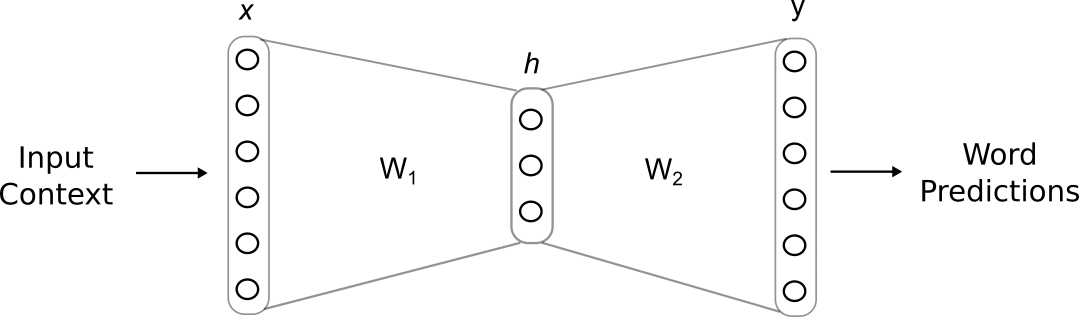
\includegraphics[width=4.5in]{figures/word2vec.png}
	\caption{Basic model architecture for learning word embeddings via prediction. A binary input vector, $x$, encodes a collection of one or more words that constitute a context. This input is then passed through a simple neural network that computes a probability distribution over words. Gradient descent is used to learn the weights $W_1$ and $W_2$ so that this probability distribution accurately reflects the likelihood of word co-occurrences in the training corpus. Embeddings for individual words correspond to the rows and columns of the weight matrices. Figure adapted from Rong (\citeyear{Rong:2014}).}
    \label{fig:w2v}
\end{figure}

In the special case where there is one target word and one context word, the CBOW and SG models are roughly equivalent. It helps to consider this case to obtain a deeper understanding of how these models work \citep[see][for further details]{Rong:2014}. Suppose a single word from a corpus is provided as the input context, $x$, and the next word in the corpus is the target for the output layer $y$.\footnote{It makes no difference to designate $x$ as the target and $y$ as the context, since both the target and the context are comprised of a single word here.} In this case, the input is encoded as a ``one-hot'' binary vector\footnote{A one-hot vector is a vector of zeros with a single element set to 1. This element corresponds to a particular feature of interest - in this case a single word.} that extracts a single column from the input-to-hidden weight matrix $W_1$. Thus, the value of the hidden layer is $h = W_1 x$, where $x$ is the binary input vector. Next, each unit in the output layer encodes a dot product between $h$ and a row in the hidden-to-output weight matrix $W_2$. The softmax function is then used to convert these dot products into a proper probability distribution. Importantly, each column of $W_1$ is treated as an embedding for a particular word, as is each row of $W_2$. The goal of learning is to make the $W_1$ embedding of a word most similar to the $W_2$ embedding of the target word that follows it in the corpus. 

At an intuitive level, the way that learning changes the model's weights is easy to understand \citep{Rong:2014}. Each row $j$ in $W_2$ is updated with values of the hidden layer activities, but scaled by both the learning rate and the prediction error at $y_j$. So, for a given output unit, if the model incorrectly guesses that the word corresponding to this unit ought to be predicted, the unit's incoming weights will be decremented to be more \textit{dissimilar} to the hidden layer vector. In effect, this lowers the value of the dot product between the first layer embedding of the input word, and the second layer embedding of the output word under consideration. On the other hand, if the model incorrectly fails to assign a high probability to the correct word, the unit corresponding to this word will have its incoming weights incremented to become more \textit{similar} to the hidden layer vector. This raises the value of the dot product between the first layer representation of the input word and the second layer representation of the correct output word. As such, when same input is provided again to the model, it will be more likely to predict the correct output. The updates to $W_1$ follow a similar but less directly interpretable pattern. Finally, the full CBOW and SG models both build on this basic procedure by either adding multiple words to the input or by attempting to predict multiple words at the output. 

\subsection{Discussion}

If talk of meaning is largely shorthand for talk of the expected effects of language use, then the idea of using continuous vectors to summarize linguistic regularities is an appealing one. An embedding can be thought of as a description of what is \textit{likely to follow} from the occurrence of a word, since measurements of embedding similarity are directly related to the conditional probability of one word appearing given another. As such, word embeddings are thematically consistent with the requirements of a semantic theory built on the idea that meanings specify certain expected consequences of language use. Understanding a language requires having a good predictive model of linguistic phenomena, and for all their simplicity, embedding models are nothing if not predictive.

It also possible to interpret embedding models as somewhat degenerate specifications of inferential roles. Prediction is a form of inference, so treating a word as a predictor of other words (as embedding models do) is equivalent to treating a word as something that licenses inferences to other words.\footnote{Strictly speaking, only sentences have inferential roles, since only sentences can be used as premises and conclusions in inferences \citep{Brandom:1994}. But prior to the discussion of compositionality in the next chapter, it is harmless to assume that words have inferential roles of the sort made explicit in conditional expressions such as ``If something is a robin, then it is a bird''.} The significance of this interpretation is that it suggests new responses to some standard criticisms of inferentialist approaches to semantics. For example, the fact that the inferential role of one expression cannot be defined independently of the inferential roles of numerous other expressions is often thought to problematically entail that no two language users share the same meanings, since no two language users will be disposed to make exactly the same inferences \citep{FodorLepore:1991,FodorLepore:2002}. Cast into the idiom of distributional semantics, the objection is that no two embedding models will possess exactly the same structure if they are generated from slightly different text corpora, and hence no two models will encode exactly the same meanings. But such models can nonetheless be highly \textit{similar} in the sense that they contain embeddings that are spatially distributed in a similar way. Moreover, it is possible to quantify this similarity such that if the models were taken to approximate human linguistic knowledge, it would be possible to make concrete estimates of the likelihood of successful communication. For instance, if two models assign the same ordinal ranking to the likelihoods of certain words co-occurring with a target word, then it's not clear that there are grounds on which to conclude that two speakers whose lexical knowledge is approximated by these models would ``misunderstand'' one another. Much more could be said here, but the point is simply to illustrate that a lot depends on the details of how one implements the notion of an inferential role. Dismissing inferentialist approaches on \textit{a priori} grounds is accordingly inappropriate.

It would nonetheless be a mistake to read too much into these models. For one thing, there is a world of difference between a word being used and a word merely occurring in particular context. Methods that aim to predict such occurrences accordingly do not explain language \textit{use} in the way that is required of theory of semantics. For another thing, these methods typically do not incorporate information that is relevant to explaining how linguistic expressions relate to the non-linguistic world. There is no in principle barrier to including such information \citep{Baroni:2014,LandauerDumais:1997}, but concrete efforts to do so are currently few and far between. Finally, the reason there has been a surge of recent interest in word embeddings has little to do with theoretical issues in semantics. Rather, embeddings have simply proven themselves to be useful ingredients in natural language processing tools such as parsers, part-of-speech taggers, and machine translation systems \citep{Manning:2015}. 

Overall, it is clear that embedding models can shed new light on longstanding issues in semantics concerning the viability of holism. But it is also clear that there remains a considerable gap between these models and a model that accurately captures the semantics of lexical items. Bridging this gap requires examining how words are combined to produce phrases and sentences.

\section{Phrase and Sentence Embeddings}

At first glance, it is not clear how to extend the distributional hypothesis to accommodate phrases and sentences. The problem is that multi-word linguistic expressions tend to be fairly unique and thus occur very rarely in the linguistic environment. Co-occurrence data then becomes highly \textit{sparse}, which makes it difficult to identify distributional regularities shared by multiple expressions \citep{Baroni:2014}. To illustrate this point with an example, it is likely that the previous sentence has \textit{never} occurred in written English before. The distributional profile of this sentence is accordingly difficult to compare to the profile of other sentences. 

However, it is possible to mitigate the effects of data sparsity by defining contexts that are shared by large numbers of distinct expressions \citep[][p. 261]{Baroni:2014}. One idea is to define these contexts in terms of words that are present in possible extensions of a target expression. For instance, the sentence ``the dog growled'' could be extended into ``the big dog growled and snapped its teeth'', which would then warrant treating the words ``big'', ``snapped'', and ``teeth'' as contexts defining the sentence's distributional profile. Another, similar idea is to use words occurring in sentences both before and after a target sentence as contexts. Interestingly, neither of these ideas has gained much popularity. Most researchers have instead chosen to develop methods for \textit{composing} the distributional profiles of words into distributional profiles for phrases and sentences \citep{Mitchell:2010,Baroni:2014}.

In what follows, I examine four approaches to composing word embeddings into phrase and sentence embeddings. The first approach uses additive operations to mix embedding components \citep{Mitchell:2010,Mikolov:2013}. The second approach uses multiplicative ``binding'' operations to join embeddings into simple role-filler structures \citep{SmolenskyLegendre:2006,Plate:2003,Eliasmith:2013,Smolensky:1990}. The third approach uses repeated applications of a single non-linear mapping to merge a set of embeddings in sequential order \citep{Elman:1990,Elman:1991}. Finally, the fourth approach generalizes the third to merge embeddings in accordance with a non-sequential structure such as a parse tree \citep{Socher:2014,Socher:2011,Tai:2015,Socher:2012,Iyyer:2014,Bottou:2014}. In addition to providing a deeper assessment of distributional approaches to semantics, this discussion helps to set the stage for a more thorough examination of compositionality in Chapter 4. 

\subsection{Additive Models}

In most early work on distributional semantics, vector addition is used as a sort of default method for producing composite embeddings. For instance, Landauer and Dumais (\citeyear{LandauerDumais:1997}) encode sentences as sums of word vectors in an effort to account for data from experiments involving assessments of paragraph coherence. Jones and Mewhort (\citeyear{JonesMewhort:2007}) similarly encode stems (i.e., multi-word prompts) as sums of word vectors in a effort to account for data from studies of constraints on stem completion. In more applied research on natural language processing, the use of vector addition to produce composite representations of sentences and documents is widespread.\footnote{Models that exploit addition to produce ``bag of words'' vector representations are often used as baselines to assess performance in tasks such as document classification. These baselines are often surprisingly hard to beat.} 

More recent work by Mitchell and Lapata (\citeyear{Mitchell:2010}) expands on this implicit use of vector addition by introducing a general class of additive composition functions. These functions all satisfy the following formula: 

\begin{equation}
v_{c} = \textrm{A}v_{s_1}+ \textrm{B}v_{s_2} 
\end{equation}

\noindent 
where $ v_{c} $ is an embedding for a complex expression, $ v_{s_1} $ and $ v_{s_2} $ are embeddings for simple expressions, and $ \textrm{A} $ and $ \textrm{B} $ are matrices (p. 1402). To provide some explanation, if $ \textrm{A} $ and $ \textrm{B} $ encode the identity transformation, then this approach is equivalent to vector addition. Otherwise, the contribution made by each constituent embedding is modulated to some degree. For instance, a head word\footnote{In linguistics, a head word is a word that provides a template of sorts into which obligatory arguments and optional modifiers are added to construct a complete phrase \citep{Pinker:1994,Harley:2014}.} might be given extra weight in the sum defining a phrase, so as to reflect its importance to the meaning of the phrase \citep{Baroni:2014}. Typical choices for $ \textrm{A} $ and $ \textrm{B} $ produce a weighted average or ``mixture'' of word embeddings \citep{Baroni:2014}.

Intuitively, these mixture models can be thought of as combining occurrence counts over contexts. For example, if the word \textit{A} occurs five times in some context while word \textit{B} occurs only two times, then the phrase \textit{AB} might be taken to occur in this context a total of seven times, or perhaps twelve times if \textit{A} is taken to be twice as important as \textit{B}. The advantage of combining contexts in this fashion is that the resulting embeddings retain information from each of their constituents. The drawback, of course, is that this information fails to capture how these constituents interact with one another. To say that an adjective-noun combination such as ``slow fish'' corresponds to an embedding that is comprised mostly of the embedding for ``fish'' does not provide much insight into the combination's distributional profile. A related problem is that function words such as ``on'' and ``the'' occur in almost every context, which means that they essentially just introduce noise into additive embeddings \citep{Baroni:2014}. Given the important semantic role played by function words, this consequence is undesirable. 

Overall, additive models tend to produce composite embeddings that cluster on the basis of weighted lexical overlap, and as such, the computed similarities tend only to capture coarse-grained topical relations. However, Mitchell and Lapata (\citeyear{Mitchell:2010}) report experimental results indicating that these relations correlate surprisingly well with human judgments of phrase similarity.  

\subsection{Multiplicative Models}

A slightly different approach to building composite embeddings emerges from early research on artificial neural networks. This work was frequently criticized for adopting representational assumptions inconsistent with the principle of compositionality \citep[see e.g.,][]{FodorPylyshyn:1988}, which prompted researchers to introduce methods for ``binding'' distributed representations together to form symbol structures \citep{Smolensky:1990,Plate:1995,Gayler:2004}. The most common method uses the tensor product\footnote{The tensor product of $ a \in R^m $ and $ b \in R^n $ is a tensor in $ R^{mn} $ whose elements are pairwise products of the elements in $a$ and $b$. It is equivalent to the outer product if $a$ and $b$ are vectors.} to produce ``role-filler pairs'' that tag particular representations to particular structural roles  \citep{SmolenskyLegendre:2006}.

Again, Mitchell and Lapata (\citeyear{Mitchell:2010}) expand on the notion of tensor product binding to introduce a general class of multiplicative composition functions. These functions all satisfy the following formula: 

\begin{equation}
v_{c} = \textrm{C} \cdot (v_{s_1} \otimes  v_{s_2})
\end{equation}

\noindent
where $ v_{c} $ is again an embedding for a complex expression, $ v_{s_1} $ and $ v_{s_2} $ are embeddings for simple expressions, $ \otimes $ is the tensor product, and $ \textrm{C} $ is tensor whose rank is greater than the rank of $ v_{s_1} \otimes  v_{s_2} $ (see pp. 1402-04 for details). If $ \textrm{C} $ is the identity, then the formula reduces back to the tensor product. If $ \textrm{C} $ is a binary tensor that extracts the diagonal of $ v_{s_1} \otimes  v_{s_2} $, then the formula is equivalent to the elementwise multiplication of $ v_{s_1} $ and $ v_{s_2} $. If $ \textrm{C} $ is a binary tensor with ones along the transdiagonal elements of its vertical ``slices'', then the formula computes the circular convolution of $ v_{s_1} $ and $ v_{s_2} $, which is equivalent to a compression of the tensor product \citep{Plate:2003,Mitchell:2010}. 

Intuitively, all of these variants can be thought of as generating occurrence counts for conjunctions of contexts. For instance, if word \textit{A} occurs in context \textit{X} two times while word \textit{B} occurs in context \textit{Y} three times, then the expression \textit{AB} is taken to occur six times in a conjunctive context \textit{XY}. In the special case where the composition function is element-wise multiplication, these conjunctive contexts are the same as the original contexts, which results in composite embeddings that accentuate points of overlap in the distributional profiles of their constituents \citep{Baroni:2014,Mitchell:2010}. Unsurprisingly, these multiplicative models have many of the same problems as their additive counterparts.

However, it is worth noting that multiplicative methods were not originally designed with the assumptions of distributional semantics in mind. Typical uses of tensor products and circulation convolution tend to define bindings between elements that are largely syntactic (i.e., roles) and elements that are largely semantic (i.e., fillers) \citep{SmolenskyLegendre:2006,Plate:2003}. Moreover, in the case of circulation convolution, binding is only guaranteed to work if the elements in each constituent vector take on values sampled from a mean-zero normal distribution \citep{Plate:2003}, which is unlikely to correspond to the occurrence statistics of any lexical item. The point here is that neither operation should be expected to combine distributional information in an intuitively plausible manner.

It is nonetheless worth pointing out that when multiplicative functions are combined with additive ones, it becomes possible to define complex symbolic structures using distributed representations. The specific choice of functions defines what is called a ``vector symbolic architecture'' or VSA \citep{Gayler:2004}. VSAs are used in cognitive models, but from a linguistic perspective, they are not entirely well-motivated \citep{Eliasmith:2013}. The problem is that a VSA defines complex linguistic expressions as collections of parts (i.e., specific role-filler bindings) that have no direct influence on one another. As will become clear, it is difficult to define inferential roles in terms of such role-filler collections. 

In all, the main drawback of both additive and multiplicative methods for producing complex embeddings is that they fail to adequately capture interactions between linguistic expressions \citep{Baroni:2014}. It is natural (and common in linguistics) to think of certain words as modifying other words. For instance, an adverb such as ``quickly'' modifies a verb it applies to by providing more specific information about the type of action the verb describes. Incorporating this kind of modification into composite embeddings requires the use of more complicated functions that operate over sequences and trees. 

\subsection{Sequential Models}

Sequential models for producing composite embeddings have their roots in research on recurrent neural networks (RNNs) in cognitive science and machine learning \citep{Elman:1990,Elman:1991}. These networks are mathematical models that map a series of inputs to a series of outputs by recursively applying a single non-linear function. Importantly, behavior of this function depends on both the current input to the network and the state of a ``hidden'' distributed representation that acts as a memory of prior inputs. The benefit of the feedback provided by this memory is that an RNN's hidden state becomes conditioned on the entire history of an input sequence. It is because of this sensitivity to input history that RNNs are used to model a wide range of sequential and temporally extended phenomena \citep{Sutskever:2014}. 

In linguistic applications, each input to an RNN corresponds to a word embedding, and the hidden state corresponds to composite embedding of all prior inputs. The recursion that defines this composite embedding is as follows:

\begin{align}
\label{eqn:rnn_hid}
h_t &= f (W^{xh} x_t + W^{hh} h_{t-1} + b) \\ 
\label{eqn:rnn_out}
y_t &= W^{hy} h_t 
\end{align}

\noindent
where $h_t$ corresponds to the current hidden state, $x_t$ corresponds to the input, $h_{t-1}$ corresponds to the previous hidden state, $b$ is a bias on the hidden state, and $f$ is an element-wise function. The matrices $W^{xh}$ and $W^{hh}$ apply transformations to the input and the previous hidden state, respectively. The output of the network, $y_t$, is then computed by applying the linear transformation $W^{hy}$ to the current hidden state.\footnote{Strictly speaking, computing a separate output from the hidden state is optional, so for simplicity I will assume that the composite embedding for a sequence of input embeddings is drawn from the hidden state.} The recurrence defined by these equations can be made more intuitive by unfolding it over a sequence to produce a chain of the sort depicted in Figure \ref{fig:rnn}. What is important to note is that equations (\ref{eqn:rnn_hid}) and (\ref{eqn:rnn_out}) define a composition function that produces embeddings with an internal structure defined by this chain, with the parameters $W^{xh}$ and $W^{hh}$ repeated at each link. Alternate composition functions that similarly unfold into a chain define alternate sequence models. A well-known example of such an alternative is the ``Long Short-Term Memory'' (LSTM) network \citep{Sutskever:2014}. 

\begin{figure}
\centering
	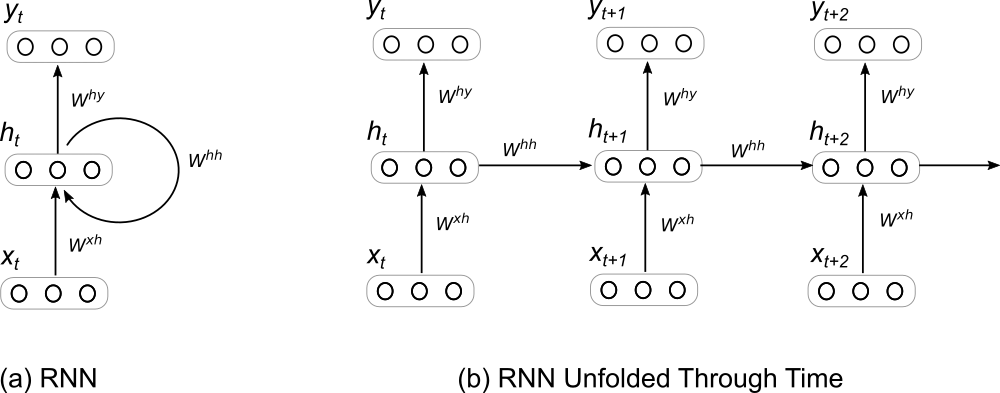
\includegraphics[width=5in]{figures/rnn.png}
	\caption{Unfolding a recurrent neural network through time. At each time step, an embedding corresponding to the current word in a sequence (e.g., a sentence) is provided as the input state $x$. The hidden state $h$ and the output state $y$ are then updated. Over time, $h$ and $y$ come to encode information about the entire history of the input sequence.}\label{fig:rnn}
\end{figure}

It is worth pointing out two things about the relationship between sequential, multiplicative, and additive models. First, if $f$ is set to the identity and $b$ is zero, then (\ref{eqn:rnn_hid}) is equivalent to an additive model that is applied over a sequence. If $W^{hh}$ is further set to compute a fixed circular convolution while $W^{hx}$ is set to the identity, then (\ref{eqn:rnn_hid}) can be thought of as implementing a VSA to produce a simple list. These observations indicate that sequential models implement some (though not all) simpler composition functions as special cases. Second, the recursive nature of these models allows them to accommodate the idea that linguistic expressions modify one another. More specifically, it is possible to think of a recurrent network as a function whose behavior is defined by its previous inputs. Thus, when a new input is presented, it is in a sense \textit{modified} by all previous inputs to yield the next state of the network. It is for this reason that RNNs have to the power to capture complex sequential dependencies between words \citep{Elman:1991,Sutskever:2014}.

Unlike most additive and multiplicative models, RNNs do not compute functions that are defined \textit{a priori}. They are instead trained to \textit{approximate} an unknown function by learning from examples of the function's inputs and outputs. Details of the training procedure can vary, but typically the backpropogation method is used in tandem with gradient descent to find a set of parameters that minimize some measure of error in the network's outputs. There are, however, two drawbacks to this kind of training when it is applied to the problem of producing embeddings for word sequences. First, examples of good multi-word embeddings are needed to provide the necessary training data. It is often not clear what such examples should look like, and even when it is, they are typically hard to come by in sufficient quantity. Second, it is difficult to interpret the hidden states of an RNN once its parameters have been optimized. The dimensions of this state typically have no direct interpretation as occurrence counts in particular contexts, which makes it unclear how to understand RNN embeddings in distributional terms. 

A more theoretical problem is that there are good reasons to think that linguistic structure is non-sequential. The possibility of arbitrarily iterated noun phrases such as ``the big dog with the leather collar with the shiny tag with the...'' that eventually combine with a verb phrase has motivated numerous views on which linguistic expressions are organized into hierarchies rather than sequences \citep{Pinker:1994,Harley:2014}. While RNNs fail to capture this hierarchical structure, they can be generalized to create fully recursive models that unfold into trees and certain other kinds of graphs \citep{Socher:2012,Socher:2014,Bottou:2014}. 

\subsection{Tree-Structured Models}

Tree-structured models differ from sequential models by defining composition functions that map variable numbers of ``child'' embeddings onto a single ``parent'' embedding. For example, the embeddings for the child words ``no'' and ``thesis'' might be mapped by a single function to produce an embedding for the parent noun phrase ``no thesis''. Further applications of this function can then be used to produce an embedding for the verb phrase ``writes itself'' from embeddings for each of its constituents, along with an embedding for the sentence ``no thesis writes itself'' from embeddings of the resulting noun and verb phrases. The advantage of these kinds of functions is that they allow word embeddings to be composed in accordance with the syntactic structure of a sentence and therefore accommodate standard linguistic analyses of the interface between syntax and semantics \citep[see e.g.,][]{Szabo:2012}. 

It is also possible to define composition functions that accommodate a variety of different of syntactic formalisms. For instance, functions defined over pairs of child embeddings are consistent with binary constituency grammars \citep{Socher:2012}, while composition functions defined over variable numbers of child embeddings are consistent with dependency grammars \citep{Socher:2014,Tai:2015}. Furthermore, the use of typed lexical embeddings (i.e., embeddings that reside in different vector spaces) can be used to define composition functions consistent with categorial grammars, wherein certain linguistic expressions are treated as functions that get applied to other linguistic expressions \citep{Baroni:2014}. A standard RNN, finally, is a special case of a tree-structured model in which the tree is binary and strictly left-branching. Figure \ref{fig:tree-rnn} illustrates examples of different tree structures and their corresponding composition functions. 

\begin{figure}
\centering
	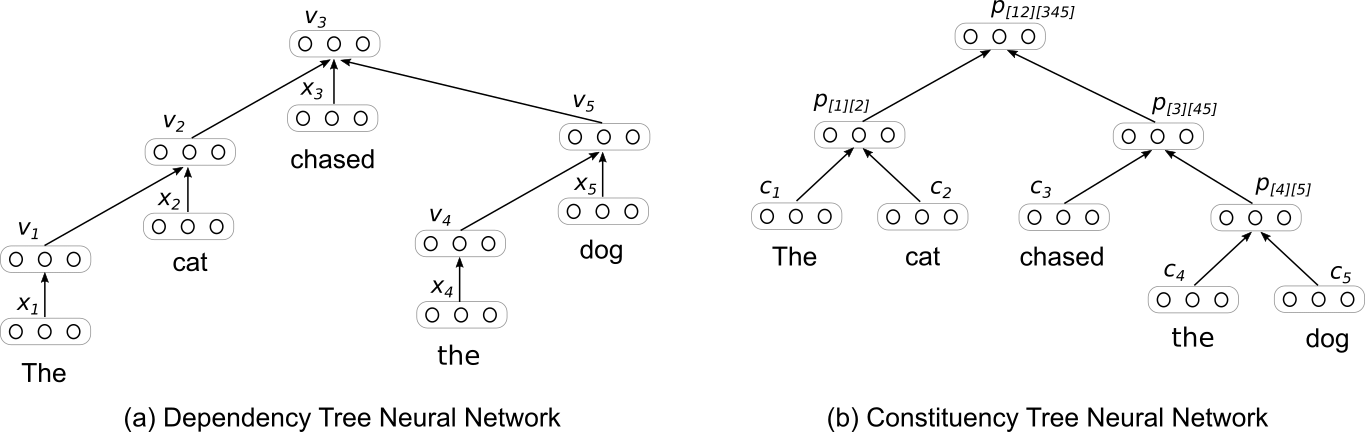
\includegraphics[width=6in]{figures/tree_comp.png}
	\caption{A comparison of dependency and constituency tree structured neural network models. In each case, a network layout is constructed from a parse of the input sentence. Constituency-based networks include layers corresponding to phrasal constituents (e.g., noun phrases), while dependency-based networks do not. Variables are labeled for consistency with the naming conventions in equations (\ref{eqn:ct_rnn}), (\ref{eqn:dt_rnn_leaf}), and (\ref{eqn:dt_rnn_nonleaf}), which formally describe how sentence embeddings are produced using each model.}
\label{fig:tree-rnn}
\end{figure}

Given that these models apply a composition function in a hierarchical manner to produce a single embedding for a sequence of words, it follows that some prior specification of the structure of this hierarchy must be provided. It is for this reason that many tree-structured models rely on external parsers to define a layout for the neural network that is used to produce a sentence embedding from a set of word embeddings \citep{Socher:2012,Socher:2014}. Once this layout is produced, it is relatively straightforward to compute embeddings for both the sentence as a whole and its various constituents. In the case of a binary constituency tree, the standard composition function used to produce these embeddings is the following:

\begin{align} 
\label{eqn:ct_rnn}
v_p = f (W [v_{lc}; v_{rc}] + b)
\end{align}

\noindent
where $v_p$ is the parent embedding, $[v_{lc}; v_{rc}]$ is the concatenation of the left child embedding and the right child embedding, $b$ is a bias on the parent embedding, $f$ is an element-wise function, and $W$ is a matrix that maps the concatenated embedding back into the space of the child embeddings. This composition function is then applied recursively to compute embeddings for each node in the tree whose children have been computed, and the recursion terminates when every node in the tree is assigned an embedding. As in the case of sequential models, an external error signal of some kind is typically used to learn the parameters of the composition function, in this case the matrix $W$ and the bias vector $b$. More complicated composition functions with larger numbers of parameters are also possible \citep[e.g.,][]{Tai:2015,Socher:2012}, provided that they map two child embeddings to a single parent embedding of the same dimensionality. 

One drawback of constituency trees is that they produce embeddings that are quite sensitive to subtle changes in word order and word choice, even if the resulting sentences are highly similar \citep{Socher:2014,Iyyer:2014}. For example, the constituency trees for passive and active variants of the same sentence are quite distict (e.g., ``Paul played the piano'' vs ``The piano was played by Paul''), which can lead a model to produce fairly dissimilar embeddings using these trees \citep{Socher:2014}. Another drawback is that embeddings at the nodes closest to the root of a constituency tree tend dominate the overall sentence embedding. This is undesirable if the nodes in question correspond to words or phrases that are minimally important to the sentence's meaning \citep{Socher:2014}.

Models that make use of dependency trees rather than consituency trees avoid most of these problems \citep{Socher:2014}. A dependency tree assigns a single node to each word in a sentence, and then introduces a set of edges (or ``arcs'') that identify which nodes depend on other nodes to be interpreted properly. A \textit{root} node that depends on every other node in the tree (either directly or indirectly) is then taken to summarize the entire sentence. A constituency tree, in contrast, has one \textit{leaf} node per word in a sentence, plus numerous intermediary nodes that correspond to phrases or phrasal constituents that eventually combine produce a root node for the sentence as a whole. So, in the case of sentence with \textit{n} words, a dependency tree will consist of \textit{n} nodes, while a binary constituency tree will consist of $2n - 1$ nodes. Dependency trees are accordingly relatively shallow in comparison to constituency trees. This can be advantageous when use training algorithms that rely on backpropogation. Example dependency and constituency trees are shown in Figure \ref{fig:tree-rnn}. 

A further advantage of using dependency trees is that the links between nodes are labeled with specific dependency relations that can be used to parameterize a composition function. Specifically, each dependency relation is associated with a specific weight matrix that is used to help determine the embedding. The assignment of embeddings to nodes in the tree then proceeds in a two-step manner. First, all of the leaf nodes in the tree (i.e., nodes that do not depend on other nodes) are assigned embeddings by applying a simple transformation to their underlying word embeddings:

\begin{align} 
\label{eqn:dt_rnn_leaf}
v_j = f (W_v x_j + b) 
\end{align}

\noindent
where $v_j$ is the embedding for the $j^{th}$ leaf node in the tree, $x_j$ is the embedding for the word corresponding to this node, $W_v$ is a matrix that transforms word embeddings, and $b$ and $f$ are a bias term and elementwise function as before. Second, embeddings are recursively assigned to all of the non-leaf nodes by composing the embeddings of their children as follows:

\begin{align}
\label{eqn:dt_rnn_nonleaf}
v_i = f (W_v x_i + b + \sum_{j \in C(i)} W_{R(i,j)} \cdot v_j )
\end{align}

\noindent
where $v_i$ is the embedding for the $i^{th}$ non-leaf node in the tree, $x_i$ is the embedding for the word corresponding to this node, $j$ is an index that ranges over the children, $C(i)$, of node $i$, and $W_{R(i, j)}$ is a matrix associated with the specific dependency relation between node $i$ and its $j^{th}$ child. $v_j$ is the embedding corresponding to this child. One thing to note about this formalization is that the composition function is invariant to changes in the order of the words corresponding to its children. For instance, encodings of the phrases ``a gray bellowing hippo'' and ``a bellowing gray hippo'' will assign identical embeddings to the head word ``hippo''. Whether or not this kind of order invariance constitutes a problem probably depends on the task to which the model is applied.

As before, the use of error-driven parameter learning requires that a model be provided with examples of desirable sentence embeddings. Most tree-structured neural networks are accordingly parameterized for a very specific task, such as predicting sentiment labels for sentences \citep{Socher:2011,Socher:2012}. This kind of task-specificity is not necessarily a problem, but it does raise the question of whether it is possible to create generic embeddings that are able to account for a wide range of semantic phenomena.

\subsection{Discussion}

Care is required in giving semantic interpretations of phrase and sentence embeddings. These embeddings typically reside in the same vector space as the word embeddings from which they are derived, so it is theoretically possible to interpret them in distributional terms. Each element of a word embedding, recall, corresponds to a measure of its likelihood to occur in an abstract context.\footnote{The contexts are abstract in the sense that they are defined through the application of a dimensionality reduction procedure to a co-occurrence matrix.} Different composition functions (i.e., additive, tree-structured, etc.) define different ways of assigning values to the elements in one vector on the basis of the values of elements in a set of \textit{other} vectors. So, there is a natural sense in which these functions determine the distributional profile for a complex expression from the distributional profiles of its simpler parts. The methods under consideration accordingly compose distributional profiles in a manner analogous to to the way in which truth-theoretic approaches compose denotations by computing the denotation of a complex expression from the denotations of its simpler parts \citep{Carpenter:1997}. 

There are two problems with this straightfowardly compositional view of sentence embeddings. First, when an error signal is used to define a composition function, the embeddings produced by this function take on values that minimize the magnitude of the error signal. So, if the error signal is not designed to produce good distributional profiles for multi-word expressions, then it is simply a mistake to interpret the resulting embeddings in distributional terms. Second, even if the error signal is described in terms of antecedently specified distributional profiles, one is still stuck with the problem of choosing appropriate contexts over which to define these profiles, as discussed in the introduction to this section. The use of nearby words as contexts does allow one to specify distributional profiles for simple multi-word expressions \citep[see][pp. 290-295]{Baroni:2014}, but this choice is poorly motivated from a theoretical perspective. Co-occurrence events involving single words essentially become primitives for semantic analysis at every level of syntactic complexity, and such primitives are surely inadequate if the goal of semantics is to explain how words and sentences function as complex tools for prediction in social contexts that involve intentional interpretation. 

The best way to think about these methods is in terms of the fact that different composition functions induce different similarity relations over the linguistic expressions for which embeddings are produced. Additive models typically define this similarity relation in terms of a weighted lexical overlap between two expressions, while multiplicative models define it in terms of prominent conjunctions of embedding elements. Both kinds of model are usually unsupervised in the sense that they are not trained to produce embeddings that satisfy some external criterion. Sequential and tree-structured models, in contrast, are neural networks that do rely on such a criterion. In standard cases, the relevant criterion is to minimize some measure of error in predicting the correct network outputs for some set of example network inputs. The inputs in this case would be sentences and the outputs might be classification judgments of some kind. By minimizing its prediction error, a model learns to approximate some undefined function from sentences to class labels, where the training input-output pairs are taken to be sampled from this function. The key point here is that the similarity relation induced over a set of linguistic expressions is determined by the specific function being approximated.

One interesting feature of these induced similarity relations is that they are all consistent with the previously mentioned idea of treating linguistic expressions as predictors of other linguistic expressions (or their properties). To explain, if a similarity relation is induced on the basis of distributional information, then measurements of embedding similarity are again related to the conditional probability of one expression appearing given another. Alternatively, if a similarity relation is induced through function approximation, then measurements of embedding similarity are related to the conditional probability that one expression gets mapped to a particular output given that another does. The difference between these two cases is that in one, expression occurrences are being predicted, while in the other, function outputs are being predicted. 

So, in keeping with the idea that describing an expression's meaning involves giving a specification of the expected effects of its use, the correct way to interpret these sentential embeddings is in terms of the role they play in regulating the functional behavior of the models in which they are defined. For instance, in an unsupervised additive model, sentence embeddings regulate predictions of sentence similarity. Similarly, in an supervised sequence model, sentence embeddings regulate predictions of sentence labels. Unfortunately, none of the models discussed here rise to the challenge of defining functional behavior that captures the pragmatic significance of uttering a linguistic expression. Again, this pragmatic significance is to be understood in terms of a sentence's inferential role, so the clear next step involves building models that predict inferential relationships between sentences.  

\section{Predicting Inferential Relationships}

As Brandom (\citeyear{Brandom:1994}) notes, semantics must answer to pragmatics (p. 83). The pragmatic significance of uttering a particular sentence is characterized by the IPA framework in terms of the effect the utterance has upon a conversation. This effect, again, determines which further claims each interlocutor can be expected to assent to, which questions they can be expected to ask, which commands they can be expected to issue, and so forth. An inferential role is then introduced to codify such effects, and thereby explain how the sentence is \textit{used} to anticipate and control the trajectory of a dialogue. Talk of meaning is accordingly talk of how linguistic expressions function as instruments of prediction in the context of intentional interpretation.  

If the distributional methods just discussed are to account for how linguistic expressions function as such instruments, then they obviously need to be extended considerably. I suggest a two step approach to performing this extension. The first step involves formulating the notion of an inferential role in terms of a function that maps a sentence onto the further sentences that follow from or contradict it. These sentences constitute a kind of ``local neighborhood'' around a target sentence within a much broader network of inferences. The second step involves approximating the function that produces this local neighborhood by using an embedding model that learns from training examples. If successful, this two step process will yield a model that is able to compute rudimentary inferential roles for arbitrary input sentences. 

The viability of this approach hinges on the use of high quality training data. In what follows, I first discuss a recently released corpus that provides such data. I then describe sentence embedding models that learn on the basis of this data to predict inferential relationships between sentences. Next, I present results that illustrate how well each model is able to predict relationships between novel sentences not seen in the training data. I conclude by illustrating how these models can be used to construct a simple inferential network around a target sentence.  

\subsection{The SNLI Corpus}

The Stanford Natural Language Inference (SNLI) corpus is a recently released dataset consisting of 570,152 sentences pairs labeled with inferential relationships \citep{Bowman:2015}. The first sentence in each pair is referred to as the \textit{premise}, while the second sentence is referred to as the \textit{hypothesis}. If the hypothesis follows from the premise, then the pair is labeled as an example of entailment. If the hypothesis is inconsistent with the premise, the pair is labeled as an example of contradiction. And if the hypothesis might or might not be true given the premise, then the pair is labeled as neutral.

Each sentence pair is generated by providing a human annotator\footnote{These annotators were recruited through Amazon Mechanical Turk. See Bowman et al. (\citeyear{Bowman:2015}) for details.} with an image caption (but not the corresponding image), and then asking them to write three further captions: one which is definitely also true of the image, one which might be true of the image, and one which is definitely not true of the image. To illustrate with an example, one initial caption is ``Under a blue sky with white clouds, a child reaches up to touch the propeller of a plane standing parked on a field of grass,'' and the annotator produced the following three additional captions: ``A child is reaching to touch the propeller of a plane'' (entailment), ``A child is reaching to touch the propeller out of curiosity'' (neutral), and ``A child is playing with a ball'' (contradiction). The use of image captions is designed to eliminate ambiguities concerning event and entity co-reference across the sentences in a given pair. Approximately ten percent of resulting pairs were subject to further validation step in which four additional annotators assigned them one of the three relationship labels. The results of this data validation suggest that inter-annotator agreement is very high, with approximately 98\% of validated sentence pairs receiving a consensus label (i.e., at least three of the five annotators are in agreement). 

Finally, the dataset is divided into a training set of 550,152 sentences pairs, a development set of 10,000 pairs, and a test set of 10,000 pairs. The training set is used to teach a model to assign the correct inferential labels to sentence pairs, while the test set is used to assess how the well the resulting model is able to assign labels to novel pairs. The development set is used to select model hyper-parameters (i.e., parameters that are not learned over the course of training, such as the embedding dimensionality). 

\subsection{Model Details}

To compare different sentence embedding models, I ran a series of experiments assessing performance on the SNLI task. Specifically, I test four models: (1) an additive model that encodes each sentence as a sum of word embeddings; (2) a multiplicative model that encodes each sentence as a collection of role-filler pairs; (3) a sequential model that encodes each sentence using an RNN; and (4) a tree-structured model that encodes each sentence using a network constructed with the help of a dependency parser. For each sentence pair, these models are used to create two sentence embeddings, which are then concatenated into a single embedding that is passed to a simple feed-forward neural network that acts as a classifier by computing a probability distribution over possible labels. Figure \ref{fig:model} illustrates this model architecture in more detail.

The models are all trained via backpropogation to learn a set of parameters for both the classifier and the sentence embedder that minimizes error on the training set. All of the models are initialized with 300 dimensional word embeddings created using the methods of Mikolov et al. (\citeyear{Mikolov:2013}). These word embeddings are then fine-tuned over the course of training. Each model was trained for approximately twenty passes over the entire training set, with the learning rate annealed by half after every three passes. The same embedding model is used for both the premise sentence and the hypothesis sentence in all cases. A description of further details concerning these experiments, along with the code used to run them, is available online at https://github.com/pblouw/pysem. 

\begin{figure}
\centering
	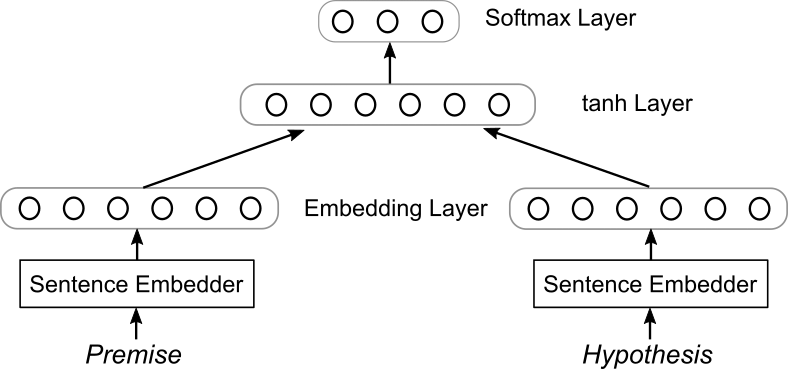
\includegraphics[width=3.8in]{figures/classifier.png}
	\caption{General model architecture for predicting inferential relationships between pairs of sentences \citep[see][]{Bowman:2015}. The premise and hypothesis sentences are each embedded using one of the models described in Section 2.4 above. The resulting embeddings are concatenated and fed into a simple neural network that performs a three-way classification (entailment, contradiction, or neutral) using a single tanh hidden layer and a softmax output layer.}\label{fig:model}
\end{figure}

\subsection{Results and Error Analysis}

The accuracy of each model on the training set and the testing set is presented in Table \ref{accuracy}. As is clear, the multiplicative model performs the worst, with the remaining models performing fairly comparably on the test data. The tree-structured model, however, is unique in that it performs very well on the training data. This high performance is almost certainly a case of overfitting, since the model has a vast number of free parameters, and since performance on the test data is comparatively low. However, it should be possible to reduce this overfitting by either (a) introducing regularization, (b) reducing the number of model parameters, or (c) increasing the amount of training data. I accordingly focus primarily on the use of this tree-structured model in what follows, since it is both linguistically well-motivated and empirically successful.

There are at least three kinds of sentence pairs that this tree-structured model tends to have difficulty with. First, if one of the sentences is extremely long, the model seems to be unable to identify information that is relevant to determining its relationship to the other sentence. For example, in the test case where the premise sentence is ``a group of young boys wearing track jackets stretch their legs on a gym floor as they sit in a circle'', while the hypothesis sentence is ``the boys in their track jackets in the gym stretch their legs'', the model incorrectly predicts a contradiction, presumably because it cannot determine whether talk of sitting or stretching in the premise sentence ought to be used to evaluate the likelihood of the hypothesis sentence. Second, if the inferential relationship between two sentences is determined by sophisticated forms of background knowledge that the model is not able to induce from the training data, then model is likely to make an incorrect prediction. For example, in the test case where the premise is ``a man in a short mohawk and beard'', while the hypothesis is ``there is a man with a ponytail and a mustache'', the model incorrectly predicts an entailment, since it has no way of knowing that a mohawk is a hairstyle that is distinct from a ponytail. Third, if an inferential relationship between two sentences is determined by complex scoping relations involving negations or quantifiers, then the model is again likely to make an incorrect prediction. In the test case where the premise is ``a group of men are sitting and standing a courtyard, some of them are reading books and some are talking'', while the hypothesis is ``a group of males are outside reading and singing'', the model incorrectly predicts an entailment, presumably because it fails to grasp that the double use of the word ``some'' splits the group into those who talk and those who read, thereby ruling out the existence of a group that both sings and reads. Improving the model's ability to handle these kinds of cases likely requires the use of a more varied selection of training data.  

\begin{table}[!t]
\begin{center} 
\caption{Model Accuracies on the SNLI Classification Task} 
\label{accuracy} 
\vskip 0.12in
\begin{tabular}{c c c c} 
\hline
Model & Parameters &  Training Set (\%)  & Test Set (\%)\\
\hline
Chance  & 0 & 33.3 &  33.7 \\
Additive & 181,200 & 79.2 & 76.7 \\ 
Multiplicative & 181,200 & 58.6 & 59.2 \\
Recurrent & 361,800 &  75.6 & 75.0  \\
Tree-Structured &  4,334,700 &  83.7 & 77.0  \\
\hline
\end{tabular} 
\end{center} 
\end{table}

One interesting feature of the model is that it can be used to iteratively construct a sentence's inferential role. The construction procedure involves applying the model to a series of sentence pairs in which some sentence of interest is held constant as either the premise or the hypothesis. The predictions of the model can then be used to build out networks of the sort depicted in Figure \ref{fig:infrole}. These predictions are not universally correct, as is shown by the fact the model incorrectly predicts an entailment relation in cases where the hypothesis sentence is very likely, but not guaranteed, to follow from the premise sentence. For example, the model predicts that the sentence ``The kids are outside'' is entailed by the sentence ``some kids are wrestling on an inflatable raft'', which discounts the possibility that the kids are in an indoor pool.

The most important thing to note about these results is that, for each premise sentence, the model places \textit{every} other possible sentence into one of three disjoint classes: one corresponding to sentences that follow from the premise, one corresponding to sentences that contradict the premise, and one corresponding to sentences that are neutral with respect to the premise. Given as much, it is reasonable to conclude that the model can be used to assign a rudimentary inferential role to every possible sentence that can be formed using a vocabulary of known words. These inferential roles may not perfectly codify the correct uses of particular sentences, but they do provide a good foundation for building towards technically rigorous approaches to semantics that follow in the use-theoretic tradition.  

\begin{figure}
\centering
	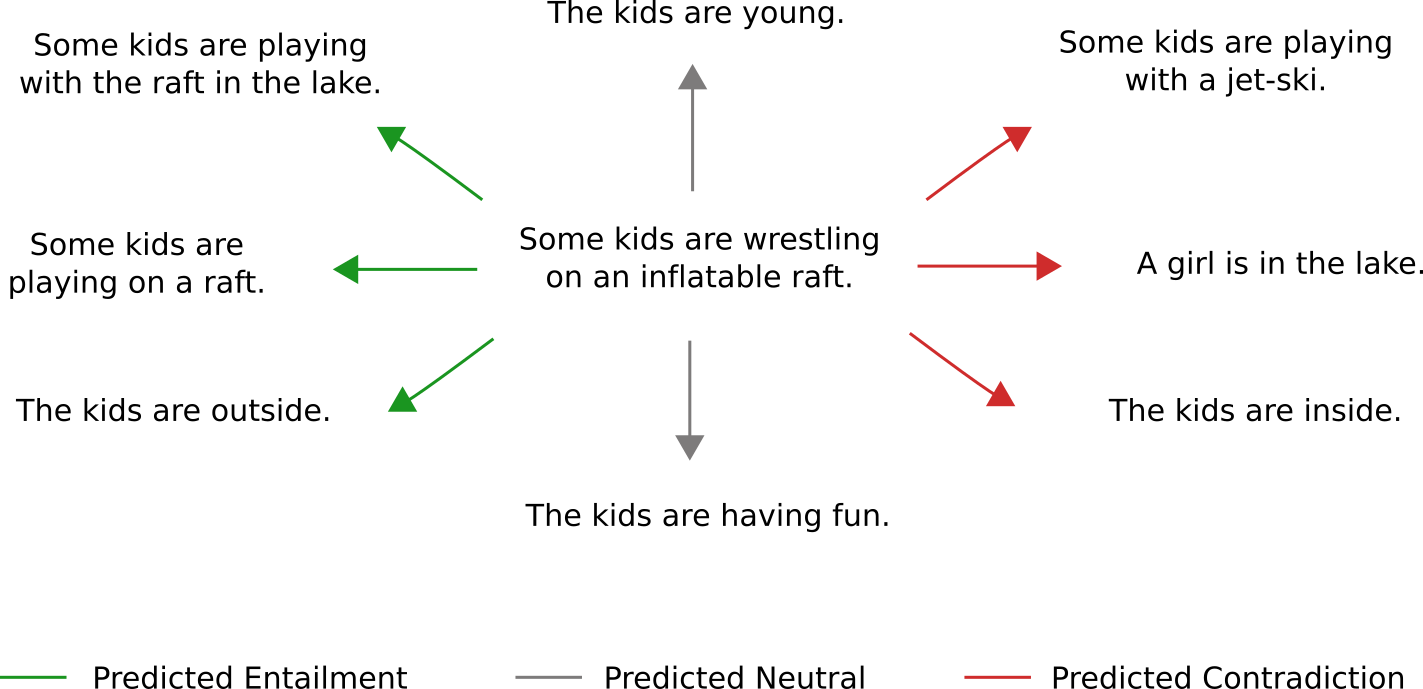
\includegraphics[scale=0.53]{figures/inf-role.png}
	\caption{A modeled estimate of part of the inferential role for the test sentence ``Some kids are wrestling on an inflatable raft.'' The network is constructed by using a tree-structured model trained on SNLI to predict a class label for each sentence pair connected by a colored arrow.}\label{fig:infrole}
\end{figure}

\subsection{Discussion}

On what grounds then is it acceptable to treat the embeddings used in these experiments as having semantic significance? An embedding for a sentence is clearly not something from which one can simply ``read off'' a meaning or a description of the world. Rather, an embedding is something that plays a functional role in a model that exhibits some kind of semantically interpretable behavior. So to answer the question: if a model's behavior can be characterized using intentional vocabulary, then it is appropriate to describe the embeddings that bring about this behavior as meaningful entities rather than mere system states \citep[see][]{Dennett:1987}. 

By this measure, the embeddings produced in the preceding experiments are somewhat semantically degenerate. A model that predicts inferential relationships between sentence pairs is subject to only a very limited form of intentional interpretation. If, for instance, the model produces an entailment prediction, then it is possible to say that the model ``thinks'' that the second sentence it was presented with follows from the first. More generic intentional state attributions are also possible. For example, the model tends to get ``confused'' by quantifiers, and it generally ``assumes'' that sentences with a large degree of lexical overlap entail one another. Such generic attributions also license high-level predictions about how the model will behave in novel situations. It is reasonable, for instance, to expect that the model will make an incorrect prediction if it is presented with lexically similar sentences with subtle quantificational differences (e.g., ``Some apples are rotten'' vs. ``All apples are not rotten''). Overall, though, this sort of intentional interpretation is a bit of stretch.

I am accordingly not arguing that the models just discussed are genuine intentional systems. Rather, I am arguing that these models codify the meanings of the sentences they process only insofar as they can be interpreted as intentional systems. Such interpretations can be more or less successful. But in the ideal limit, if a model can accurately determine what a sentence follows from, what follows from it, and what it rules out, then it counts as genuinely understanding what the sentence means \citep{Brandom:1994}. Meeting this standard of competence is exceedingly difficult, but the models I have just described arguably offer a step in the right direction. And insofar as these models count as comprehending certain sentences, I think it is fair to conclude that the models codify the \textit{meanings} of these sentences. Why? Because the models provide a formal specification of what ought to be expected from the use of particular sentences in terms of various inferential relations. Such a specification, as argued in Chapter 1, is exactly what a theory of meaning aims to provide.

\section{Conclusion}

There is no exact logic of ordinary language, but to admit as much is not to deny the possibility of technically sophisticated analyses of the behavior of linguistic expressions. To give an account of an expression's meaning is to provide a specification of the expected consequences of its use, and the results described in this chapter illustrate how such specifications can be made mathematically precise in terms of embedding models that inferentially relate sentences to one another. More specifically, error-driven function approximators can be used to induce functions that accurately predict inferential relationships between arbitrary pairs of sentences. These functions can also be used to iteratively construct a simple network of inferential relations involving a target sentence, as shown in Figure \ref{fig:infrole}. The goal of the next chapter is to build on this foundation by introducing more sophisticated models that are capable of realizing a broader range of intentionally interpretable behavior. 


\chapter{Inferential Roles Made Explicit}
%======================================================================
\renewcommand{\epigraphrule}{0pt}
\setlength{\epigraphwidth}{4.5in}
\epigraph{\textit{Logical vocabulary endows practitioners with the expressive power to make explicit as the contents of claims just those implicit features of linguistic practice that confer semantic contents on their utterances in the first place.}}{- Robert Brandom, 1994}

\section{Introduction}

It is a significant challenge to build a model that engages in intentionally interpretable behavior involving the use of natural language. One way to approach this challenge is to start with a model that a supports only a specific class of intentional state attributions, such as attributions of \textit{understanding} that concern specific linguistic expressions. Such attributions are in turn supported by the ability to infer what a given sentence follows from and is followed by \citep{Brandom:1994}. For example, to understand the sentence ``The dancers parade down the street,'' a model must be able to infer that the dancers are outside, that they are not standing still, that there is likely a surrounding audience, along with a variety of other things. And since understanding a sentence involves understanding its \textit{meaning}, it follows from this view that the meaning of an expression is determined by the inferences it licenses \citep{Brandom:1994,Sellars:1953,Sellars:1954,Brandom:2000,Brandom:2009}. 

An important feature of this view is that it tightly couples the meaning of a linguistic expression to the role the expression plays in practices that involve intentional interpretation. It is accordingly possible to derive an explicit characterization of an expression's meaning from the structure of a model that can be successfully interpreted using intentional vocabulary. To explain, if a model can be correctly attributed an intentional state of the form ``\textit{X} understands \textit{Y}'', then the inferential behavior of the model that licenses this attribution essentially charts out the inferential role that constitutes the meaning of the expression \textit{Y}. As such, one way to achieve the goal of a technically rigorous inferential role semantics is to build an intentionally interpretable model that draws the same inferences that a competent language user would.

To work towards this goal, I introduce a neural network model that learns to generate sentences that are the inferential consequences of its inputs. The model functions by first encoding a sentence into a distributed representation, and then decoding this representation to produce a new sentence. The encoding procedure involves dynamically generating a tree-structured neural network of the sort depicted in Figure \ref{depnet}. Once a sentence encoding is produced using this network, it is fed through an ``inverse'' tree-structured network to produce a predicted sentence. Interestingly, different inverse or decoding networks can be used to generate different sentences from a single encoding. To train the model parameters (i.e. the network weights shared across different tree structures) I use the Stanford Natural Language Inference (SNLI) dataset \citep{Bowman:2015}. Overall, the purpose of the model is to formally specify or ``make explicit'' the inferential roles of arbitrary linguistic expressions \citep{Brandom:1994}. The model achieves this purpose by assigning a likelihood to every sentence that is a potential inferential consequence of its input. 

In what follows, I first describe the model and then empirically evaluate its ability to produce plausible entailments for sentences unseen in its training data. I present experimentally produced plausibility ratings for a random collection of generated sentences, and from these ratings conclude that the model captures something important about the inferential roles of ordinary linguistic expressions. Next, I provide a number of more qualitative evaluations of the model that involve (a) iterating its predictions to produce chains of inferences \citep{Kolesnyk:2016}, (b) performing word-level input substitutions to determine the inferential significance of subsentential expressions \citep{Brandom:2000,Brandom:1994}, and (c) conditioning the model's predictions on additional inputs in the form of simple prompts and questions. I then provide a discussion of possible extensions of the model that would enable it to function as a more sophisticated intentional system \citep{Dennett:1991,Dennett:1987}. I conclude that if such extensions were realized, the model's behavior would be largely indistinguishable from that of a competent speaker who knows the meanings of all the expressions that make up a particular language.

\section{Model Architecture}

The model itself is a variant of the tree-structured neural network described in Chapter 2. For this reason, I briefly review the details of these networks before introducing the specific architecture I use to generate the inferential consequences of arbitrary input sentences. The basic idea behind this architecture, familiar from machine learning research on sequence transduction \citep{Sutskever:2014}, is to use one neural network to ``encode'' a sentence into an embedding, and use a second neural network to ``decode'' a new sentence from this embedding. Here, the aim is to make the decoded sentence be an inferential consequence of the encoded sentence. Related ideas can be found in the work of Iyyer et al. (\citeyear{Iyyer:2014}) and Kolesnyk et al. (\citeyear{Kolesnyk:2016}).

\subsection{Tree-Structured Models Revisited}

To start, recall that a tree-structured neural network is designed to merge distributed representations of words into distributed representations of phrases and sentences \citep{Socher:2012,Socher:2014}. Three steps are involved in this process. First, a parser is used to derive a parse tree from some sentence of interest. Second, this tree is transformed into a neural network by replacing its edges with weights and its nodes with layers of artificial neurons. Third, activation is propagated up the tree by providing input to layers that correspond to certain nodes, as shown in Figure \ref{depnet}. The input at each node is typically a distributed representation or ``embedding'' corresponding to a single word \citep{Mikolov:2013,TurneyPantel:2010,Sahlgren:2008}.

\begin{figure}[t]
\begin{center}
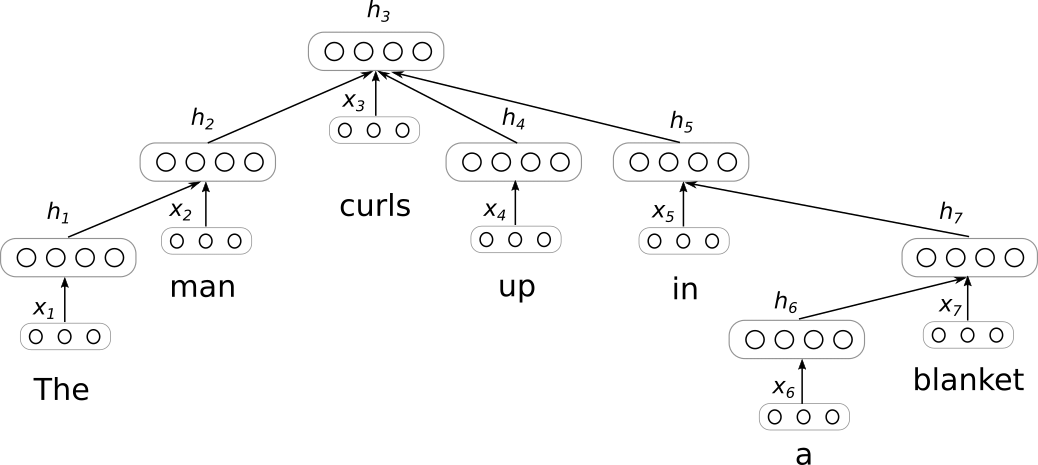
\includegraphics[width=4in]{figures/depnet.png}
\end{center}
\caption{Sentence encoding with a dependency-based tree-structured neural network. A dependency parser is used to produce the computational graph for a neural network, which is then used to produce an embedding of a sentence by merging embeddings of individual words. Figure adapted from Socher et al. (\citeyear{Socher:2014}).} 
\label{depnet}
\end{figure}

It is possible to apply these methods using arbitrary tree structures, and I adopt a dependency-based syntax in the experiments described below. There are three reasons for this choice \citep{Socher:2014}. First, the assignment of different network weights to different dependency relations allows for the creation of networks that are more sensitive to syntactic information. Second, the semantic role of an individual word can often be read off of the dependency relation it bears to a head word, which allows for the creation of networks that are also sensitive to semantic information. Finally, dependency trees are less sensitive to arbitrary differences in word order, which helps to ensure that simple variations of a sentence get mapped to similar distributed representations. The specific model I adapt -- the dependency-based tree-structured neural network -- is introduced in Socher et al. (\citeyear{Socher:2014})

It is worth briefly summarizing the process by which this model is used to generate sentence embeddings. First, an input sentence $s$ is converted into a list of pairs, such that $s = [(w_1, x_1)...(w_n, x_n)]$, where $w$ is a word and $x$ is the corresponding word embedding. Next, a dependency parser is used to produce a tree that orders the words in the sentence in terms of parent-child relations. Each node in this tree is then assigned an embedding, $h_i$, in a two-step manner that is described more formally in the previous chapter. First, all of the leaf nodes in the tree (i.e. nodes that do not depend on other nodes) are assigned embeddings by applying a simple transformation to their underlying word embeddings. Second, embeddings are recursively assigned to all of the non-leaf nodes by composing the embeddings of their children. So, in the example tree in Figure \ref{depnet}, the embeddings for nodes 1, 4, and 6 would be computed first, since these nodes have no children. Then, embeddings will be computed for any nodes whose children now all have assigned embeddings (in this case, nodes 2 and 7). And so on, until an embedding is computed for every node.

Model training is done via backpropogation and requires that a cost function be defined for the sentence embeddings produced at the root of each tree. The free parameters are the weights and biases associated with each dependency, along with a single embedding matrix $W_v$. Word embeddings can also be fine-tuned over the course of training. The number of dependency relations, and hence the number of weight matrices in the model, depends on the specific syntactic formalism that is used. In the experiments described below, 45 dependency relations define the syntax that is used by the model's parser.

\subsection{Cost Functions For Entailment Generation}

Choosing an appropriate cost function for a tree-structured neural network can be difficult, since it is not always clear what makes for a ``good'' sentence embedding. It is accordingly common to see tree-structured networks applied to narrow classification tasks such as the prediction of sentiment ratings \citep[e.g.,][]{Socher:2012}. My goal is to define an optimization objective that accounts for the principle that understanding a linguistic expression involves drawing certain inferences.

To accomplish this goal, I define a model composed of two tree-structured networks, one that encodes an input sentence into a distributed representation, and another that decodes this representation into a new sentence that is entailed by the input sentence. This model is inspired by Iyyer et al.'s (\citeyear{Iyyer:2014}) work using tree-structured networks analogously to autoencoders, but introduces a decoding procedure that computes an appropriate response to the input sentence, rather than merely reconstructing it. Figure \ref{decoder} provides an illustration of this pairing of encoder and decoder networks.

The model is trained on pairs of sentences standing in entailment relations. A dependency parser\footnote{I use the SpaCy python library, available at https://spacy.io} is used to produce a tree-structured network for each sentence, but the network associated with the second sentence is run in reverse, as shown in Figure \ref{decoder}. A word prediction is generated at each node in this second tree using a softmax classifier, which makes it possible to define a cross-entropy loss over nodes and trees as follows: 

\begin{align}
J(\theta) = - \sum_{i} \sum_{j} t^{(i)}_j \log{ p(c^{(i)}_j | s_i)}
\end{align}

\noindent
where $t^{(i)}_j$ is the target probability (i.e. 1) for the correct word at the $j^{th}$ node in the $i^{th}$ training example, $p(c^{(i)}_j | s_i)$ is the computed probability for this word given the input sentence $s_i$, and $\theta$ is the set of combined parameters for the encoder and decoder networks. Intuitively, this cost function penalizes model parameters that fail to assign a high joint probability to the collection of word predictions in the decoder that correspond to the correct entailment for a given input sentence. More formally, the training objective is to maximize the log probability of the example entailments provided in the training data. 

\begin{figure*}[t]
\begin{center}
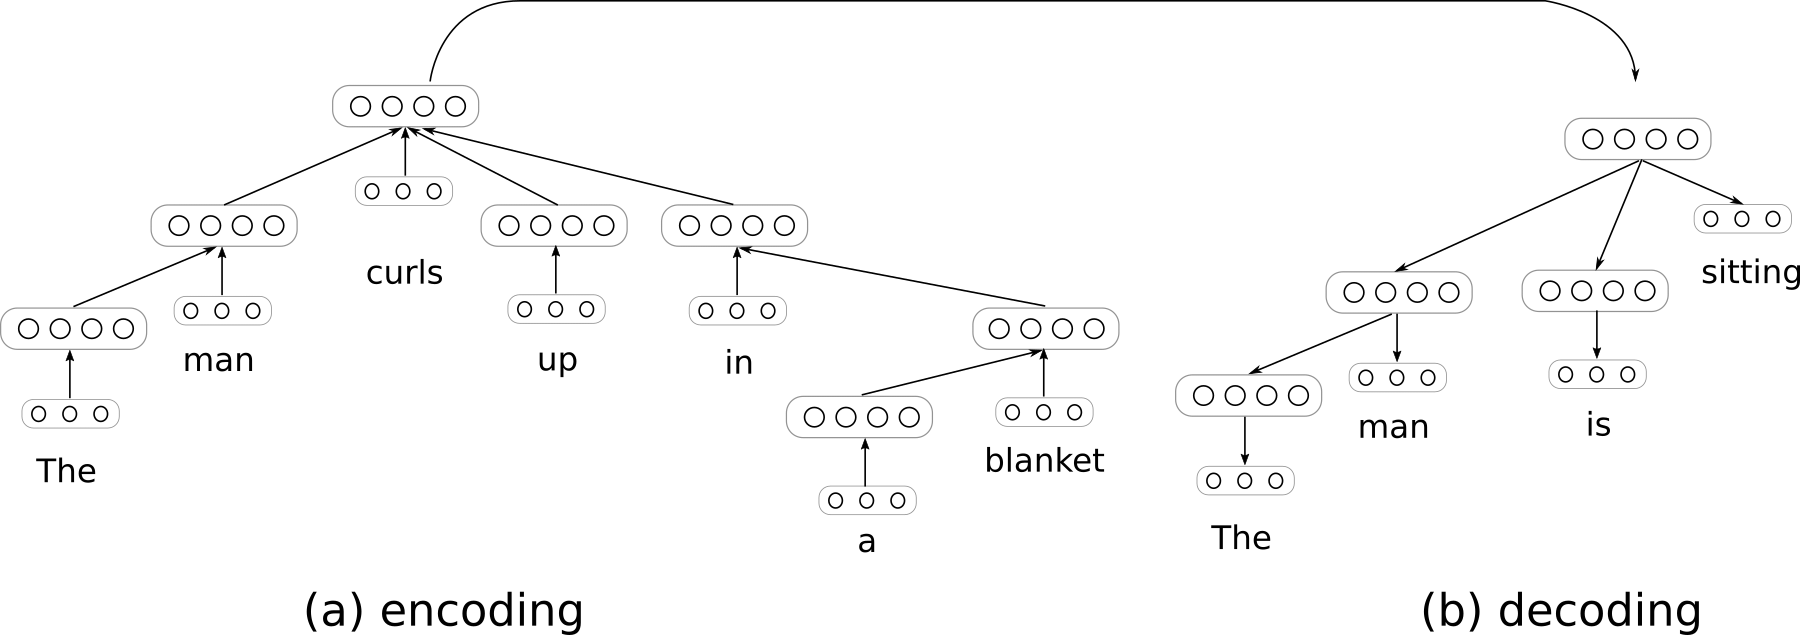
\includegraphics[width=5.5in]{figures/decoder.png}
\end{center}
\caption{Generating entailments with paired encoder and decoder neural networks. The decoder network computes a probability distribution over words at each node, conditioned on the sentence representation produced by the encoder. The parameters of both the encoder and decoder are trained via backpropogation through structure using error derivatives supplied at each node in the decoding tree. The encoder and decoder trees are dynamically generated for each pair of sentences in the training data. During inference, it is possible to use different decoding trees to generate different entailments from a single sentence encoding.} 
\label{decoder}
\end{figure*}

I train the model via stochastic gradient descent by backpropogating through both the decoder and encoder tree for each training example. The result of training is a set of weights associated with dependencies for both encoding and decoding, a set of weights for predicting a distribution over words from a node embedding for each dependency, the bias $b$ in each network, and the input transformation matrix $W_v$. When the trained model is used to perform inference using a novel input sentence, the encoder network is assembled into a tree using the learned encoding weights. The decoder network is then also assembled into a tree using the learned decoding weights, and activation is propagated through the encoder and into the decoder to produce a probability distribution over words at each tree node. The words with the highest probability at each node are then used to construct the predicted entailment for the input sentence. The tree structure for the decoder can either be selected randomly or stipulated ahead of time. 

\section{Experiments}

To evaluate the model, I perform a number of experiments that illustrate how it assigns inferential roles to arbitrary linguistic expressions. The first experiment provides a quantitative assessment of how well the model is able to learn from examples of correct inferential transitions between sentences. Specifically, for a set of novel test sentences, I measure the percentage of correct word-level predictions relative to the ``ground truth'' entailments for these test sentences present in the dataset. The second experiment provides an empirical assessment of the plausibility of entailments generated by the model for a random selection of novel test sentences. Very roughly, human subjects are asked to rate the likelihood that model-generated entailments are true given that the sentences provided as inputs to the model are also assumed to be true. Together, these two experiments provide a fairly rigorous measure of how well the model is able to generate sentences that are the inferential consequences of its inputs.

The remaining assessments of the model are accordingly more qualitative in nature. The third experiment, following Kolesnyk et al. (\citeyear{Kolesnyk:2016}), involves iterating the encoding-decoding procedure to generate chains of entailments from a given input sentence. Interestingly, this sort of iteration can be used to explicitly build out inferential roles for arbitrary input sentences, as illustrated in Section \ref{sec:iteration} below. The fourth experiment involves substituting individual words in an input sentence to identify whether the model is able to ``interpolate'' between known examples of correct inferential transitions to produce novel transitions that are nonetheless correct. A further goal of this substitutional analysis is to evaluate the extent to which the model is able to learn word-level indirect inferential roles of the sort discussed by Brandom (\citeyear{Brandom:1994}). The final experiment is the most speculative in nature, and is designed to condition the model's generation of an entailment on a further input such as a prompt or a question. The goal of this experiment is to evaluate the extent to which the model is able to selectively navigate the inferential roles is assigns to particular sentences. If successful, this kind of selective navigation provides a foundation for more complicated forms of question-answering that many researchers take to be at the core of intelligence \citep{Weston:2015,Weston:2016}. 

\subsection{Model Training}

To train the encoder and decoder components of the model, I use a subset of the SNLI dataset \citep{Bowman:2015}. Each pair of sentences in this dataset is labeled with a particular inferential relationship, as discussed in the previous chapter. Since my interest is in generating entailments, I only consider pairs labeled with the entailment relation. To reduce the amount of noise and complexity in the dataset, I also perform some simple pre-processing. First, I screen for misspelled words,\footnote{I use the PyEnchant python library, available at http://pythonhosted.org/pyenchant/.} and eliminate all sentence pairs containing a misspelling. The resulting vocabulary for the model consists of 25,550 words. Second, I eliminate all sentence pairs containing a sentence longer than 15 words in order to avoid fitting model parameters to a small number of very long sentences that produce highly complex dependency trees. After preprocessing, the data consists of a 106,288-pair training set, a 1701-pair development set, and 1666-pair test set. The training set is used for learning model parameters, while the development set is used to tune hyperparamters such as the learning rate and the number of training epochs.

\begin{table}[!t]
\begin{center} 

\caption{Examples of Entailments Generated From Novel Test Sentences.} 

\label{examples}
\vskip 0.06in
\setlength{\tabcolsep}{12pt}
\begin{tabular}{ll} 
\hline

\multicolumn{1}{c}{\rule{0pt}{3ex} INPUT SENTENCE} & 
\multicolumn{1}{c}{GENERATED ENTAILMENT} \\

\hline
% \setlength{\tabcolsep}{1pt}
\rule{0pt}{3ex}The man in colorful shorts is barefoot. & The man is wearing his shorts. \\
A young man sleeping next to a dog. & A man is near a dog. \\
The 3 dogs are cruising down the street. & The dogs are on the street. \\
Woman reading a book with a grocery tote. & A woman with book is reading. \\
\hline
\end{tabular}
\end{center} 
\end{table}

Prior to training, the word vectors that are used as input to the encoder are initialized as 300-dimensional word2vec embeddings \citep{Mikolov:2013}. Each set of weights associated with a syntactic dependency is initialized as a $300 \times 300$ identity matrix with mean-zero Gaussian noise for both the encoder and decoder. The word transformation matrix, $W_v$, is initialized in the same way. During learning, all of these matrices are updated using stochastic gradient descent, along with the word2vec embeddings. Approximately 10 passes through training data are performed using an initial learning rate of $2 \times 10^{-4}$. The learning rate is progressively annealed over the course of training.

As an initial illustration of the kind of model performance this training results in, Table \ref{examples} provides some examples of entailments produced for sentences drawn from the SNLI test set. The decoding trees used to produce each of these entailments are chosen randomly, which indicates that the model is capable of learning to produce sentences with novel syntactic properties. It is also worth noting that each example here is only the \textit{most probable} entailment given a particular decoding tree. It is therefore theoretically possible to compute ranked collections of entailments with each decoding tree.  

\subsection{Evaluating Entailment Accuracy}

Recall that the SNLI corpus consists of pairs of sentences, and that the first sentence in each pair is referred to as the ``premise'' while the second sentence is referred to as the ``hypothesis''. In the procedure just described, the model is essentially learning to predict the hypothesis paired with each example premise in the training data. It is therefore possible to measure how accurately the model performs this task. Specifically, one can measure the proportion of nodes in the model's decoder for which the predicted word is the same as the correct word in the relevant hypothesis sentence. A caveat is that the tree for this sentence must be provided to the decoder, such that input activities are propagated through paired trees of the sort depicted in Figure \ref{decoder}, where the decoder tree is the correct tree for the conclusion of the inferential transition being considered.

When applied to the training set, this accuracy measure indicates the extent to which the model has ``memorized'' the example inferential transitions it was presented with during learning. When applied to the test set, the measure indicates whether the model has learned something that allows it to correctly predict specific inferential transitions in novel situations. It is worth noting that this measure is not entirely ideal in the case of the test set, since the model might generate a plausible entailment from a premise sentence that is non-identical to the specific entailment that is present in SNLI. It is also worth noting that prior work involving SNLI has almost uniformly focused on the problem of classifying sentence pairs. As such, I cannot easily draw comparisons to earlier work.

\begin{table}[!t]
\begin{center} 
\caption{Word-Level Accuracy for Entailment Generation} 
\label{accuracy} 
\vskip 0.12in
\begin{tabular}{c c c} 
\hline
Model  &  Training Set (\%)  & Test Set (\%)\\
\hline
\rule{0pt}{3ex}Chance  &  6.0 &  5.9 \\
Encoder-Decoder  &  66.7 & 61.8  \\
\hline
\end{tabular} 
\end{center} 
\end{table}

The results of computing entailment generation accuracies on the both training and test sets are presented in Table \ref{accuracy}. A baseline accuracy computed by chance is also reported. The model performs considerably better than chance, both because it has a large number of free parameters and because it is able to use syntactic information to condition its word predictions on part-of-speech information implicit in the structure of a decoding tree. For example, if the tree requires a particular word to be a determiner, then the number of plausible candidate words shrinks drastically, since there are only a handful of determiners in English (e.g., ``the'', ``a'', etc.). The model also generalizes surprisingly well to novel test sentences, with a fairly limited drop in accuracy.\footnote{If the model were merely memorizing the example inferential transitions present in the training data, then this drop would likely be much higher due to overfitting.} One point to note concerning this generalization is that extremely high accuracies on the test set are not entirely desirable, since they would indicate that the model has learned to exclusively predict a specific inferential transition for each input sentence. However, there are numerous examples of correct inferential transitions involving such sentences, and the model should ideally be learning to assign a high likelihood to all of them.  

Overall, the fact the model can generate the example inferential transitions in SNLI with a fairly high degree of accuracy provides good initial evidence that it is able to codify the inferential roles of ordinary linguistic expressions. Examples of the sort listed in Table \ref{examples}, moreover, suggest that these inferential roles are comprised of well-formed sentences that a competent speaker of English could readily understand. 

\subsection{Evaluating Entailment Plausibility}

One limitation of the assessments just described is that they do not provide a quantitative measure of how plausible or comprehensible the sentences produced by the model are. I therefore perform a simple study in which human subjects are asked to evaluate the plausibility of model-generated sentences. During the study, participants are shown a series of sentences introduced as true captions of unseen images.\footnote{Recall that all of the sentence pairs in SNLI were generated by providing subjects with a caption for an unseen image and asking them to produce a further caption that is either true, false, or maybe true of the image. So all of the sentences in SNLI can be described as image captions. The point of using this caption-based strategy in the construction of the dataset is to eliminate co-reference ambiguities that make it difficult to determine the appropriate inferential relationship between two sentences. See Bowman et al. (\citeyear{Bowman:2015}) for more details.} For each caption, the participants are shown an alternate caption and asked to evaluate the likelihood that it is also true of the corresponding image. Evaluations are recorded using a five point Likert scale that ranges from ``Extremely Unlikely'' (1) to ``Extremely Likely'' (5). The original caption in each case is the first sentence in a pair randomly chosen from the SNLI test set, while the alternate captions are either (a) model-generated entailments, (b) human generated entailments drawn from the test set, or (c) human generated contradictions also drawn from the test set. Participants are divided into three separate conditions corresponding to each type of alternate caption. This between-subjects experimental design is similar to the method used by Bowman et al. (\citeyear{Bowman:2015}) to validate human-generated sentence pairs during the creation of SNLI. The main difference is that model-generated sentences are evaluated in addition to human-generated sentences. 

\begin{table}[!t]
\begin{center} 
\begin{threeparttable}

\setlength{\tabcolsep}{16pt}

\caption{Plausibility Ratings for Inferential Relations.} 
\label{ratings} 
\vskip 0.12in
\begin{tabular}{c c c} 
\hline
Source & Status &  Mean Likert Rating (1-5) \\
\hline
\rule{0pt}{3ex}Human & Entailment  &  4.05  $\pm$ 0.09 \\
Model & Entailment  &  3.53 $\pm$  0.12 \\
Human & Contradiction & 2.05 $\pm$ 0.12 \\

\hline
\end{tabular}
\begin{tablenotes}
      \vskip 0.06in
      \footnotesize
      \item\centering * Margins are bootstrapped 95\% confidence intervals.
\end{tablenotes}

\end{threeparttable}
\end{center} 
\end{table}

Seventy-five participants from the United States were recruited through Amazon's Mechanical Turk and split evenly into the three conditions.  The main captions were identical across conditions, and each participant was asked to rate 20 caption pairs.\footnote{Two of the main captions had no associated contradictions in SNLI, so subjects in the contradiction condition only rated 18 captions.} Participants were paid \$1.00 for their time. Two participants failed to complete the study and did not have their responses included in the results. Repeat participation was blocked by screening Mechanical Turk worker IDs. 

The Likert ratings collected during the study are assessments of the plausibility of the inferential transition from one sentence (the main caption) to another (the alternate caption). The transitions involving sentence pairs drawn directly from SNLI offer a kind of gold standard for both good and bad transitions. The results shown in Table \ref{ratings} indicate that model-generated transitions are seen to be almost as plausible as the gold-standard transitions drawn from SNLI. As such, this study provides important evidence in support of the claim that the model is able to capture certain tacit inferential relationships between natural language expressions: the inferential relationships charted out by the model are seen to be nearly as truth-preserving as those charted out by competent language users. 

\subsection{Iteration Analysis}\label{sec:iteration}

Once an input sentence has been passed through the model to generate an entailment, it is possible to use this entailment as a new input to the model. Repeated applications of the model accordingly make it possible to chart out an ``inferential network'' around a particular starting sentence. Figure \ref{inf-gen} presents a simple example of an inferential network in which the sentence ``Some kids are wrestling on an inflatable raft'' is mapped onto a number of its inferential consequences. An important difference between this inferential network and the one shown in the previous chapter is that this network is generated directly from a single input sentence. Before, the network was constructed by testing large numbers of candidate sentences to see whether they are predicted to follow from a given input sentence. Figure \ref{chain} presents a slightly different example in which various sentences describing men doing things outdoors are eventually mapped onto the sentence ``A man is outdoors''.

\begin{figure*}[t]
\begin{center}
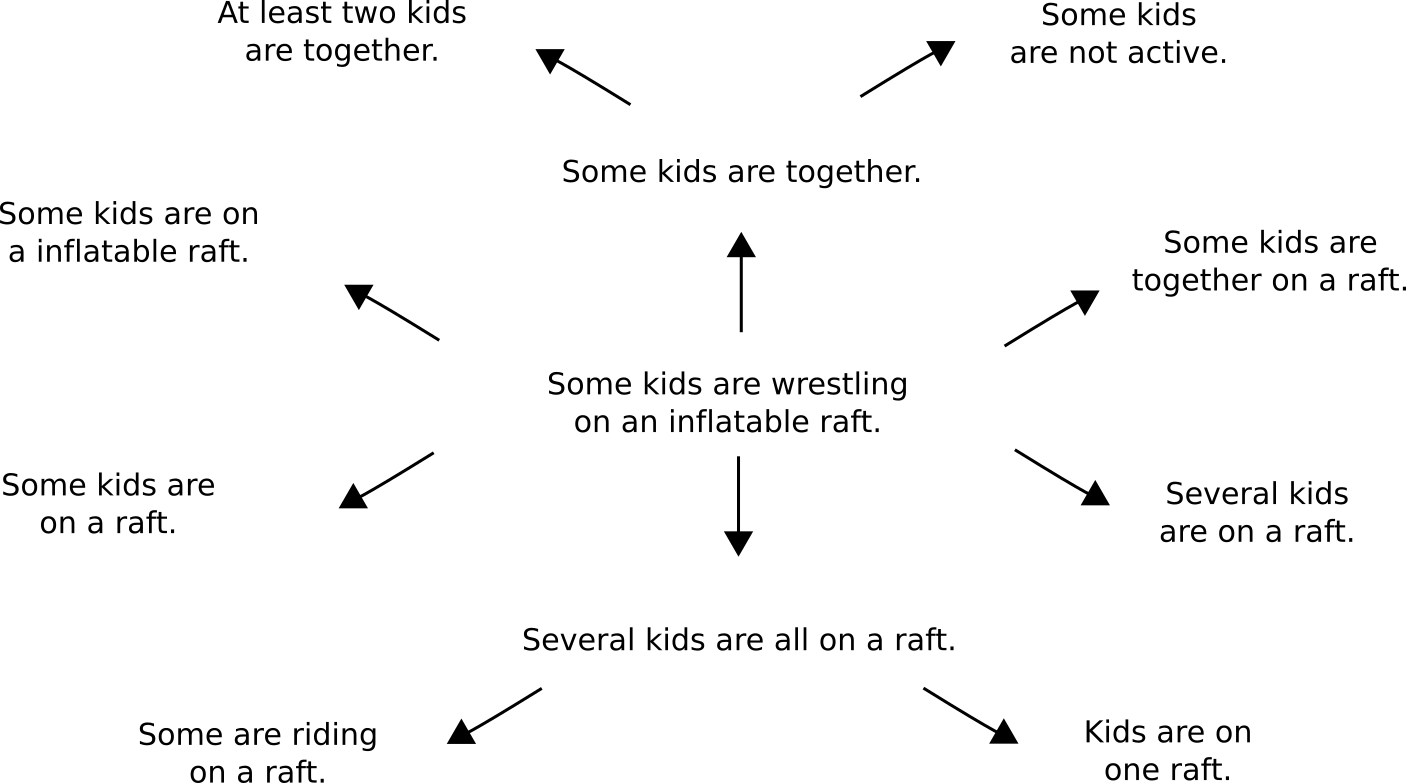
\includegraphics[width=5in]{figures/outward-inf-gen.png}
\end{center}
\caption{A model-generated inferential network around the sentence ``Some kids are wrestling on an inflatable raft''. Each inferential transition is the result of generating a predicted entailment after encoding the sentence at the beginning of each arrow. The entire network is generated starting with only the initial sentence at the center of the diagram, which is drawn from the SNLI test set. Different decoding trees are used to generate the different entailments from the initial sentence.} 
\label{inf-gen}
\end{figure*}

Two general points can be made here. First, iterative applications of the model can be used to either generate sentences that are (a) increasingly specific, or (b) increasingly general \citep{Kolesnyk:2016}. If a predicted entailment is longer than the input sentence, then it tends to describe a more specific situation. For instance, the sentence ``A bird is in a pond'' can be used to generate the sentence ``A little bird is outside in a small pond'' by using a decoding tree with nodes for two additional adjectives and an additional adverb. If a predicted entailment is shorter than an input sentence, then it tends to describe a more general situation. For instance, the sentence ``A little bird is outside in a small pond'' can be used to generate the sentence ``A bird is outside'' by using a simple decoding tree with four nodes. 

Second, these capacities for specification and generalization suggest that the inferential transitions codified by the model can be either inductive or deductive in nature. For example, the inference from ``A bird is in a pond'' to ``A little bird is outside in a small pond'' is not strictly truth-preserving and therefore inductive. The inference from ``A little bird is outside in a small pond'' to ``A bird is outside'', on the other hand, \textit{is} strictly truth-preserving and therefore deductive. Interestingly, none of these inferences are formal in the sense that they are licensed strictly by the structure of the input sentence. Rather, they are examples of what Sellars (\citeyear{Sellars:1954}) and Brandom (\citeyear{Brandom:1994}) refer to as \textit{material} inferences, or inferences that are licensed solely by a linguistic expression's meaning. 

\begin{figure*}[t]
\begin{center}
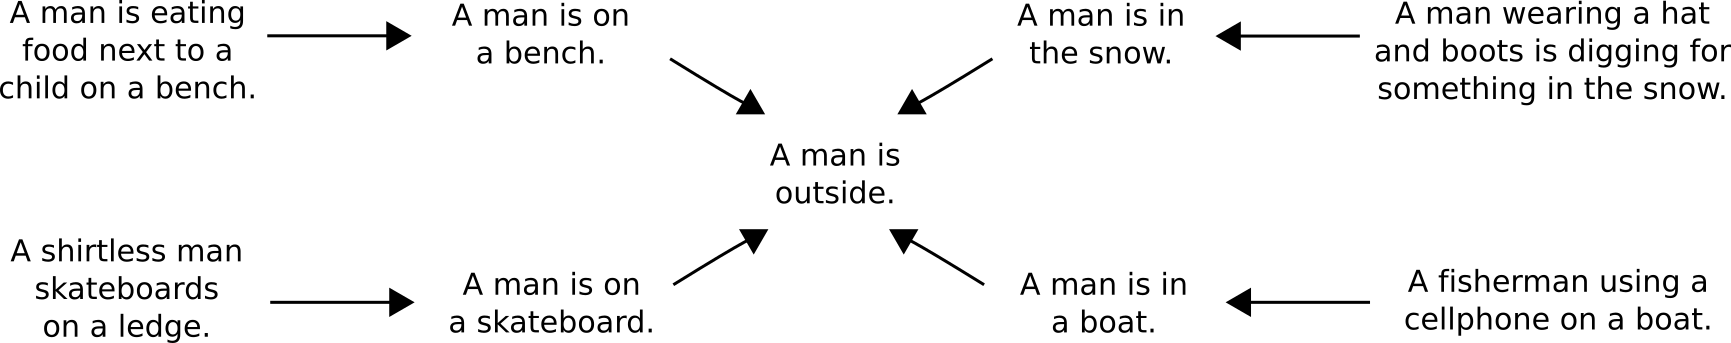
\includegraphics[width=6in]{figures/chain.png}
\end{center}
\caption{A model-generated inferential network around the sentence ``A man is outside''. Each inferential transition is the result of generating a predicted entailment after encoding the sentence at the beginning of each arrow. The entire network is generated starting with only the four outermost sentences, which are drawn from the SNLI test set.} 
\label{chain}
\end{figure*}

The most important lesson to draw from this examination of iterative prediction is that it illustrates how the model assigns an inferential role to every possible expression that can be formed from the words in its vocabulary. To explain, the model maps each input sentence onto a set of predictions concerning its inferential consequences. The model can then be used to map each sentence in this set to produce further predictions \textit{ad infinitum}. As such, it is possible to use the model to build networks of the sort shown in Figures \ref{inf-gen} and \ref{chain} for all possible input sentences. These networks, in turn, are explicit representations of the inferential roles the model assigns to particular sentences. Overall, since the model does not change as it is used to create these networks, it is fair to say that it defines an inferential role semantics for the entirety of the language that can be formed from the model's vocabulary. 

Of course, nothing guarantees that this semantics is appropriate for \textit{all} of the sentences in the language under consideration. It would be rather miraculous if a simple model trained on one hundred thousand entailment pairs managed to \textit{always} generate correct inferential transitions in novel scenarios. There is nonetheless some degree of fit between the inferential roles defined by this model and the inferential roles that govern the use of ordinary language. The goal of model development, then, is to steadily improve this degree of fit. Two changes are likely necessary to yield any substantial improvements. First, a much larger amount of training data must be made available to the model. The example inferential transitions in SNLI are somewhat idiosyncratic, and it is accordingly desirable to introduce training data that is reflective of the full range of inferential transitions that a competent language user would be inclined to make. Second, a more complex model architecture may be needed to take advantage of this additional training data. Neural networks are prone to ``catastrophic forgetting'' wherein the learning associated with newer training examples simply overwrites the learning associated with older ones. It is therefore possible that the specific model used in this experiment would not scale effectively with larger amounts of training data. Regardless, examining the use of different model architectures and larger amounts of training data is a task left for future research.

\subsection{Substitution Analysis}

Proponents of inferential role semantics typically characterize the meanings of individual words in terms of their effects on the inferential roles of the sentences in which they occur \citep{Brandom:1994,Brandom:2000,Block:1986}. The ``indirect'' inferential role associated with a particular word is then analyzed by swapping it into and out of a variety of different sentences to observe the resulting changes to the kinds of inferences that are licensed by these sentences \citep{Brandom:1994}. Interestingly, the model introduced here can be used to perform this kind of analysis in a quantitative manner. If individual words in the model's input sentence are replaced, it becomes possible to identify the impact these words have on the inferential transitions that the model predicts. In Table \ref{tab:sub}, for instance, the replacement of a subject noun or a main verb in an input sentence can be seen to have significant effects on the kinds of entailments that are generated by the model. 

\begin{table}[!t]
\begin{center} 

\caption{Substitution Analysis for ``A boy in a beige shirt is sleeping in a car''} 

\label{tab:sub}
\vskip 0.06in
\setlength{\tabcolsep}{12pt}
\begin{tabular}{ll} 
\hline

\multicolumn{1}{c}{\rule{0pt}{3ex} INPUT SENTENCE} & 
\multicolumn{1}{c}{GENERATED ENTAILMENT} \\

\hline
% \setlength{\tabcolsep}{1pt}
\rule{0pt}{3ex}A boy in a beige shirt is sleeping in a car. & A boy is sleeping in his car. \\
A girl in a beige shirt is sleeping in a car. & A girl is sleeping in her car. \\
A man in a beige shirt is sleeping in a car. & A man is sleeping in his car. \\
A woman in a beige shirt is sleeping in a car. & A woman is sleeping in her car. \\
A man in a beige shirt is driving in a car. & A man is driving a car. \\
A person in a beige shirt is selling a car. & A person is selling a car. \\
\hline
\end{tabular}
\end{center} 
\end{table}

There are two ways to think about the significance of this substitutional manipulation of the model's behavior. On the one hand, substitution can be used to assess how well the model is able to ``interpolate'' between the example inferential transitions it was trained on. To explain, any two sentences in the training data can be treated as substitutional variants of one another, provided that enough substitutions are made.\footnote{I include insertions and deletions, which can be thought of as substitutions involving the empty string.} For example, the sentence ``The dog chased after the cat'' is a substitutional variant of ``The woman drove the car'' -- ``dog'' is swapped for ``woman'', ``chased'' is swapped for ``drove'', ``after'' is swapped for the empty string, and ``cat'' is swapped for ``car''. If both of these sentences are part of inferential transitions found in the training data, then it is possible to evaluate how the model generalizes beyond these transitions by testing it on inputs that are the substitutional intermediaries of the original sentences. On the other hand, substitutions can also be used to identify specific inferential patterns that are associated with particular expression types (e.g., pronouns, quantifiers, etc.). Such patterns constitute what Brandom (\citeyear{Brandom:1994}) refers to as a subsentential expression's ``indirectly inferential role'' (p. 449). 

A main benefit of identifying indirect inferential roles is that many of the phenomena that semanticists have traditionally analyzed in truth-conditional terms can be re-analyzed in inferential terms. For example, one can test whether the model generates appropriate entailments for input sentences involving standard quantifiers like ``some'' and ``every.'' Similarly, one can test whether the model generates appropriate entailments for input sentences that exhibit anaphoric relations involving pronouns that vary with respect to gender and plurality (e.g., ``he'' vs. ``she'' vs. ``they'', etc.). Further tests involving expressions that vary with respect to numerals (e.g., one, two, many, etc.) are also possible. It is not reasonable to expect the model to pass all of these tests, since there are relatively few examples of inferential transitions in SNLI that are directly driven by quantification, anaphora, or numerosity. Nonetheless, the model exhibits some promising behavior with respect to these expression types.

In the case of quantifiers, the model is able to infer that ``some'' and ``many'' require nouns within their scope to take the plural form in an entailed sentence, as shown in Table \ref{tab:quantifiers}. The model is also able to infer that ``some'' entails ``at least one'', as shown in Figure \ref{inf-gen}. In the case of pronouns, the model is sensitive to cues that determine the gender of a pronoun in relation to its anaphoric antecedent. For example, the model correctly infers that girls and women should be referred to with female pronouns, while boys and men should be referred to with male pronouns, as shown in Table \ref{tab:sub}. In the case of numerals, the model exhibits an ability to infer appropriate quantities from simple groupings and conjunctions. For instance, the model generates a sentence containing the phrase ``Two kids...'' from a sentence containing the phrase ``A boy and a girl...'' in Table \ref{tab:quantifiers}. Finally, the model appears to have difficulty with negations. In Table \ref{tab:quantifiers}, for example, the model incorrectly infers ``A boy is not indoors'' from ``A boy in a red shirt is waiting in a store.'' While these results are rather limited, it is worth emphasizing again that the model was not designed or trained to account for phenomena involving quantifiers, pronouns, and numerals specifically. So the fact that the model's predictions are appropriately sensitive to these expressions in some cases suggests that it provides a solid foundation for developing more sophisticated analyses of specific linguistic constructions. 

\begin{table}[!t]
\begin{center} 
\caption{Substitution Analysis with Quantifiers, Numerals, and Negations} 
\label{tab:quantifiers} 
\vskip 0.06in

\setlength{\tabcolsep}{13pt}
\begin{tabular}{ll} 
\hline

\multicolumn{1}{c}{\rule{0pt}{3ex} INPUT SENTENCE} & 
\multicolumn{1}{c}{GENERATED ENTAILMENT} \\

\hline
\rule{0pt}{3ex} Some men in red shirts are waiting in a store. & \quad The men are in a store. \\
Many women in red shirts are waiting in a store. & \quad The women are in a store. \\
A boy and a girl are waiting in a store. & \quad Two kids are indoors. \\
A boy and a girl are waiting in a playground. & \quad Two kids are outside. \\
A boy in a red shirt is sleeping in a car. & \quad A boy is not outside. \\
A boy in a red shirt is waiting in a store. & \quad A boy is not indoors. \\
\hline
\end{tabular}

\end{center} 
\end{table}

Overall, the extent to which this sort of substitutional analysis can be used to define the meanings of individual words is an open question. Words are typically only used in the context of sentences, and sentences, I've argued, have meanings insofar as they license certain inferences. It is accordingly plausible that words have meanings insofar as they help determine which inferences are licensed by the sentences they occur in. Strictly speaking, I endorse this line of reasoning, but it can be misleading if one only considers inferences that relate linguistic expressions to one another, to the exclusion of inferences that relate linguistic expressions to non-linguistic perceptions and actions. In the case of a word like ``crayon'', for instance, it would be inadequate to postulate a meaning that merely codifies inferential relations amongst crayon-related sentences while saying nothing about how people identify and use crayons. A more detailed discussion of this topic is provided in Chapter 6, but for now, suffice it to say that purely linguistic inferential roles of the sort formalized in this chapter are at the very least a necessary component of an expression's meaning.

\subsection{Conditioned Entailments}

Up to this point, the association of particular inferential roles with particular sentences has not lead to any concrete explanations of facts concerning the \textit{use} of these sentences. To build towards such explanations, I briefly examine various methods for conditioning the model's predictions on additional inputs. The idea is to selectively navigate the inferential role associated with a particular sentence so as to provide appropriate answers to specific questions about the sentence. To illustrate with a hypothetical example, consider the sentence that was used to motivate the predictive adequacy criterion in Chapter 1: ``The boy waited for the pitch and then hit the ball over the fence.'' Providing an answer to a question such as ``Where did the ball go?'' or ``What did the boy likely use to hit the ball?'' involves drawing one inference amongst the many that are licensed by the original sentence. More generally, every answer to a question about this particular sentence is simply a different sentence specified by its inferential role.

\begin{table}[!t]
\begin{center} 
\caption{Prompts with ``A shirtless man sleeps in his blue boat out on the open waters''} 
\vskip 0.15in
\label{prompt} 

\setlength{\tabcolsep}{25pt}
\begin{tabular}{ll} 

% \multicolumn{2}{c}{SENTENCE: \quad A shirtless man sleeps in his blue boat out on the open waters.} \\
\hline

\rule{0pt}{3ex} PROMPT & \qquad \qquad \quad GENERATED ENTAILMENT \\

\hline
% \setlength{\tabcolsep}{1pt}
\rule{0pt}{3ex}\quad Water & \qquad \qquad A shirtless man is in the blue water.\\
\quad Blue & \qquad \qquad A blue man is in the blue boat. \\
\quad Fishing & \qquad \qquad A shirtless man fishing in the blue water. \\
\quad Sleep & \qquad \qquad A shirtless man sleeps in the blue water. \\
\quad Boat & \qquad \qquad A shirtless boat boat in the blue boat. \\
\hline
\end{tabular}
\end{center} 
\end{table}

There are two reasons why question answering is worth exploring in detail. First, the matter of whether a model can adequately perform simple forms of question answering is highly relevant to determining whether or not it can be appropriately described using the vocabulary of intentional systems theory. Put simply, a system that \textit{understands} a particular linguistic expression will undoubtedly be able to answer certain questions about it. Given that I argued in Chapter 1 that the expectations set out by inferential roles are what make intentional interpretation possible,\footnote{The idea, recall, is that intentional state attributions only license certain behavioral predictions because the sentences invoked by these attributions have particular inferential roles.} it is important to verify that my model can be subjected to such interpretation. Second, an examination of question answering allows for a clear connection to be drawn between the inferential roles assigned to particular expressions and the \textit{use} of those expressions. For example, the assignment of an inferential role to a sentence suffices to explain, amongst other things, how it gets used in simple question-and-answer dialogues.

As an initial test of the model's ability to generate conditioned entailments, I supplement its input with simple prompts consisting of single words. The resulting change to the encoding procedure is quite minimal. First, an input sentence is converted into an embedding using the usual tree-structured encoder. Second, a word embedding corresponding to a prompt is added to this embedding. The resulting sum is then passed through the decoder to produce a predicted entailment. The effect of this process is to subtly shift the input sentence embedding towards the prompt embedding in the hope that this shift will be reflected in the prediction of an entailment that is appropriate to the prompt. Table \ref{prompt} illustrates some examples of the kinds of the entailments that the model predicts under these conditions.  

The natural next step is to use complete questions instead of single word prompts to condition the model's predictions. To take this next step, I simply modify the encoding procedure to produce \textit{two} sentence embeddings using two separate encoding trees. The first embedding corresponds to an input sentence, while second embedding corresponds to a question. These embeddings are then simply added together before being passed to the decoder network. The hope, again, is that shifting the input embedding towards the question embedding will force the decoder to predict and entailment that is an answer to the question. An important caveat is that the model was not trained to perform this task, so there is little reason to suppose that it will produce appropriate answers. As Table \ref{query} indicates, the answers the model provides in response to questions are often not particularly illuminating or coherent. Nonetheless, these answers are occasionally on the right track, as in the case of the first example in the table.

\begin{table}[!t]
\begin{center} 
\caption{Queries with ``A mother and daughter walk along the side of a bridge''} 
\label{query} 

\vskip 0.07in
\setlength{\tabcolsep}{8pt}
\begin{tabular}{ll} 

% \multicolumn{2}{l}{SENTENCE: \qquad \quad A mother and daughter walk along the side of a bridge.} \\
\hline

\rule{0pt}{3ex} QUERY &  GENERATED ENTAILMENT \\

\hline
% \setlength{\tabcolsep}{1pt}
\rule{0pt}{3ex}How many people are walking? & Two people are walking.\\
 Are the mother and daughter walking? & The mother and daughter walking outdoors.  \\
 What is the bridge over? & A people are on the bridge. \\

\hline
\end{tabular}
\end{center} 
\end{table}

Overall, these tests are merely suggestive, but they point towards the development of more sophisticated models for which performance on conditional inference tasks is incorporated directly into the training objective. Developing such models will undoubtedly require training data comprised of numerous example question-answer pairs for each input sentence of interest. There are currently a number of engineering-driven efforts to build systems that learn to answer questions about short collections of text \citep[e.g.,][]{Weston:2015,Weston:2016,Sukhbataar:2015}, but these efforts have not lead to the creation of publicly available datasets of the required sort.

\section{Consequences for Semantic Theory}\label{sec:consequences}

Collectively, the experiments just described paint a somewhat mixed picture of the model's performance. On the one hand, the model is able to predict appropriate entailments for a wide range of novel sentences. There is accordingly a clear sense in which the model satifies the goal of ``making explicit'' the inferential roles of these sentences. On the other hand, the model struggles to generate entailments that are appropriately sensitive to the presence or absence of certain subsentential expressions. The model also struggles to selectively generate entailments in response to specific prompts and questions. These shortcomings are important because they demarcate the limits within which the intentional stance is predictive of the model's behavior. To explain, the model can be attributed a very rudimentary understanding of certain linguistic expressions, but it clearly cannot be attributed the full-fledged understanding possessed by a competent language user. It is a system that, in Dennett's terms, only ``sort of'' understands the sentences it is presented with \citep[qtd. in][]{Rothman:2017}.

``Sort of'' understanding a sentence is not nothing, but neither is it everything. So it is worth considering what further characteristics the model would need to possess in order to count as a full-fledged comprehender, or an intentional system comparable in nature to a linguistically competent human being. Arguably, these further characteristics fall into three general categories. First, true comprehenders are able to draw appropriate inferences on the basis of multiple pieces of information. If, for example, a person is told a simple story, they will be able to draw inferences about this story as a whole. So a model that understands language would similarly need to be able to draw ``multi-premise'' inferences involving simple narratives. Second, true comprehenders are able to draw inferences that involve non-linguistic perceptions and actions. If, for example, a person is told that a wet dog is in the house, they will expect to see drops of water on the floor. So a model that understands the sentence ``A wet dog is in the house'' would similarly need to be able to relate this sentence to certain non-linguistic observations. Finally, true comprehenders are able to effectively deploy language in a wide variety of conversational scenarios. They can ask and answer questions, respond to directions, and provide instructions, along with many other things. So a model that understands language would similarly need to be able \textit{use} language effectively in all such contexts.

It is useful to briefly speculate on some strategies for introducing these characteristics into a model. In the case of multipremise inferences, one option is to provide the model with a memory to store information about multiple sentences. The generation of an entailment could then be conditioned on \textit{all} of the sentences stored in the memory, rather than just a single sentence. A variant of this basic strategy has been developed in the recent machine learning literature on question answering systems, wherein ``memory networks'' are used to store information about simple stories and then answer certain questions amount them \citep{Weston:2016,Weston:2015,Sukhbataar:2015}. One drawback of this research is that it is not motivated by theoretical concerns about semantics. Rather, it is driven primarily by engineering considerations.

In the case of inferences that involve non-linguistic perceptions and actions, one option is to provide the model with a visual system that converts images into embeddings that can then be passed through the decoder to generate a predicted entailment. Likewise, one could provide the model with a motor system that uses sentence embeddings to generate specific actions. The idea in both cases is to extend the model to perform what Sellars (\citeyear{Sellars:1953}) refers to as ``language-entry'' and ``language-exit'' transitions, which are distinct from the ``language-language'' transitions formalized here. Interestingly, there are a number of available templates for building models that account for these further transitions. Socher et al. (\citeyear{Socher:2014}), for instance, describe a model that uses a tree-structured neural network in tandem with a convolutional neural network to match images to linguistic descriptions of their contents. On more a cognitive level, Eliasmith et al. (\citeyear{Eliasmith:2012}) describe a neurocomputational model that performs a variety of tasks that involve responding to visual images with specific motor behaviors. There are accordingly a number of tools available for building models that codify complex inferential roles spanning the domains of language, perception, and action. 

Finally, in the case of inferences that guide conversational activity, the obvious strategy is to first provide the model with the ability to perform a range of actions and then develop a training paradigm in which the model learns to perform specific actions in specific situations. For instance, the model could learn an action policy for which questions are responded to with answers, while commands are responded to with actions that fulfill them. The idea, in short, would be to construct a model that learns to make the moves involved in a variety of different ``linguistic dances.'' There are some basic templates for this sort of research. For example, reinforcement learning techniques have recently been used to build models that learn highly complicated action policies for accomplishing certain goals \citep{Mnih:2015}. It is conceivable that analogous policies could be learned for carrying out the kinds of cooperative joint actions that are fundamental to language use.

Overall, there is no easy way to build a model of the sort I am envisioning, yet it is instructive to imagine it. By hypothesis, the model would be a genuine intentional system, capable of understanding language at a human-like level, and of playing the ``game of giving and asking for reasons'' \citep{Brandom:1994}. Now consider a question: if this model provides a complete formal specification of the role that a given linguistic expression plays in regulating its behavior, would there be any facts about the \textit{meaning} of this expression that the specification leaves out? On the assumption that the model's behavior is that of a competent language user, it is plausible that there are no such facts. Put simply, if one has an explicit definition of the role that a particular linguistic expression plays in determining the behavior of intentional systems that use it, then one has an explanation on hand of all relevant facts concerning the expression's use. The definition would thereby satisfy the explanatory goals of semantic theory outlined in Chapter 1. 

\section{Conclusion}

In summary, the point of this work is to motivate an approach to semantics based on inferential relationships \citep{Brandom:1994}. The use of the encoder-decoder model is designed to illustrate how generalized inferential roles can be learned for arbitrary linguistic expressions from examples of how sentences are distributed as tacit ``premises'' and ``conclusions'' in a space of inferences. It is accordingly possible to characterize this work as an extension to the well-known distributional approach to semantics \citep{TurneyPantel:2010}, wherein the generic notion of a linguistic context is replaced with the more fine-grained notion of an inferential context. 

As with most natural language generation systems, many of the sentences produced by the model are defective in some way. As can be seen in the examples in Tables \ref{prompt} and \ref{query}, model-generated entailments are almost always thematically appropriate, but sometimes contain agreement errors or misplaced words that render the entailment as a whole ill-formed. And, not infrequently, the model produces entailments that are more or less incomprehensible. There are two ways to address these problems. The first involves the use of increased amounts of training data to provide the model with a more points in the ``space of inferences'' to interpolate between. The second involves the use of more sophisticated network architectures that help the model to learn to more selectively make use of only the input information that is most relevant to generating a good entailment. LSTM network architectures, such as the Tree LSTM \citep{Tai:2015}, are likely to provide improvements on this second front. 

Finally, an important limitation of this work is that it does not directly consider the relationship between linguistic expressions and the non-linguistic world. A natural way to account for this relationship is to suppose that a sentence's occurrence in the linguistic environment licenses certain expectations about what can be seen, heard, or otherwise perceived. To return to my initial example, if one understands the statement ``The dancers parade down the street'', one will expect to see and hear dancers upon going to the relevant street. I accordingly suggest that if an individual can adequately infer all that follows from a given linguistic expression, both linguistically and non-linguistically, then there is nothing further they need to be able to do to count as \textit{understanding} what the expression means.


%---------------------------------------------------------------------
% MAIN BODY
%----------------------------------------------------------------------
\externaldocument{chapter3}
%======================================================================
\chapter{Compositionality Reconsidered}
%======================================================================
\renewcommand{\epigraphrule}{0pt}
\setlength{\epigraphwidth}{4.5in}
\epigraph{\textit{It is enough if the sentence as whole has meaning; thereby also its parts obtain their meanings.}}{- Gottlob Frege, 1884\footnotemark} \footnotetext{Quoted in Szabo (\citeyear{Szabo:2012})}

\epigraph{\textit{...it looks as if when someone says ``Bring me a slab!'', he could mean this expression as one long word corresponding indeed to the single word ``Slab!'' Then can one mean it sometimes as one word, and sometimes as four? And how does one usually mean it? I think we'll be inclined to say: we mean the sentence as one consisting of four words when we use it in contrast to other sentences such as ``Hand me a slab'', ``Bring him a slab'', ``Bring two slabs'', etc.}}{- Ludwig Wittgenstein, 1953}

\section{Introduction}

The principle of compositionality states that the meaning of a complex expression is fixed by its syntactic structure and the meanings of its simpler parts \citep{Szabo:2013,Szabo:2012,FodorLepore:1991}. In the study of natural language semantics, this principle is typically taken to entail that expressions such as phrases and sentences are interpreted in the following two-step manner \citep{Recanati:2012}: first, a set of a lexical rules are used to assign meanings to simple expressions; then, a set of composition rules are used to combine these simple meanings into the meaning of a phrase or sentence. A compositional semantics for a language is accordingly given by a finite number of instances of the following two rule schemes \citep[pp. 175-76]{Recanati:2012}:


\begin{enumerate}
  \item $ I(e) = m $
  \item $ I(f(e_1, e_2)) = g(I(e_1),I(e_2)) $
\end{enumerate}

\noindent
where \textit{I} is an interpretation function that maps an expression \textit{e} to some entity that constitutes its meaning, \textit{f} is a syntactic operation that combines simple or complex linguistic expressions, and \textit{g} is semantic operation that maps the meanings of the inputs to a syntactic operation to the meaning of its output \citep{Szabo:2012}. Conventional wisdom states that if natural languages were not compositional in the manner spelled out by (1) and (2), it would be impossible to explain the capacity of language users to produce and comprehend indefinitely large numbers of sentences.

There are at least three significant assumptions built into this characterization of compositionality. The first assumption is that lexical meanings are explanatorily prior to sentence meanings. One cannot, in other words, give a characterization of the meaning of a sentence in the absence of some independent characterization of the meanings the words it is comprised of. The second assumption is that meanings are entities of some kind. A semantic theory is thereby tasked with the job of pairing linguistic expressions with the entities that constitute their meanings. The third assumption is that semantic interpretation is rule-based. Once the conditions for the application of a composition rule are satisfied, all interpretations inconsistent with the rule's consequences are eliminated from consideration.   

Arguably, all three of these assumptions are mistaken. The problem with giving explanatory priority to words is that words have no pragmatic significance in isolation from the sentences in which they occur \citep{Brandom:1994}. Since it is impossible to give non-sentential explanations of word use, the idea that word meanings are fundamental is a non-starter. The problem with treating meanings as entities is that the pairing of an entity with an expression is generally insufficient to provide any insight into the expression's use. Moreover, this ``pairing'' view falsely suggests that the meaning of a one linguistic expression can be specified without reference to other linguistic expressions. Finally, the problem with treating semantic interpretation in rule-based terms is that, empirically speaking, there are essentially no inviolable regularities governing the behavior of linguistic expressions \citep{SmolenskyLegendre:2006,Manning:2015,Seidenberg:1997}. Hence, there should be no strict rules involved in the characterization of these expressions' meanings. 

The preceding considerations point to a significant tension between semantic theories that are compositional and semantic theories that actually do the job of explaining language use. To help resolve this tension, I propose to translate the question of how meanings compose into the question of how people are able to generalize to the use of expressions beyond those that they have had direct exposure to. The motivation for adopting this strategy is simple: existing arguments to the effect that natural languages are compositional largely take the form of inferences to the best explanation, in which the phenomenon to be explained is the evident generality of our capacities for linguistic comprehension \citep{Szabo:2013,Szabo:2012}. As such, my main claim in this chapter is that debates about the principle of compositionality \textit{are really about generalization rather than semantic composition per se}. I then build on this claim to provide an account of linguistic generalization that makes no appeal to rules like (1) and (2).

In what follows, I first analyze some standard arguments in favor of the principle of compositionality. I conclude that these arguments do little to show that the semantics of natural language is well accounted for by a system of rules like (1) and (2). I then discuss three kinds of generalization --- similarity-based, syntactic, and procedural --- that are potentially relevant to explanations of how people extrapolate on the basis of prior experience to the correct usage of novel linguistic expressions. I assess the degree to which each of form of generalization is relevant to explanations of language use. On the basis of this assessment, I provide a positive account of linguistic generalization that is consistent with both the IPA framework and the formal properties of the model discussed in the previous chapter. Specifically, I argue that the ability to correctly use a realistically large number of linguistic expressions requires: (a) the ability to assimilate sentences in terms of similarities between the inferential contexts in which they occur; (b) the ability to assimilate subsentential expressions on the basis of similarities between the substitution-inferential contexts in which they occur; and (c) the ability to generalize certain procedures involved in language processing. The result is an account that emphasizes the explanatory priority of inferential relations amongst sentences, and that describes procedures through which these relations are determined in novel contexts via a kind of ``interpolation'' between familiar examples of correct inferential transitions. This interpolation is characterized in procedural terms, and gives rise to exactly the sort of generalization that I claim is at the core of debates about compositionality.

\section{Arguments in Favor of Compositionality}

An interesting feature of arguments in favor of the principle of compositionality is that they almost all appeal to apparent facts about the psychological capacities of language users to \textit{understand} certain classes of linguistic expressions \citep{Szabo:2013}. This is somewhat puzzling given that theorists who uphold the principle also tend to claim that the study of semantics is best pursued by abstracting away from the psychological characteristics of language users \citep[e.g.,][]{Speaks:2014,Lewis:1970,Lewis:1975,Carpenter:1997}. Even more puzzling is the fact that theorists who invoke these arguments rarely, if ever, provide a substantive account of what qualifies as understanding a linguistic expression \citep{Szabo:2013}. As will become clear, these oversights render the standard arguments in favor the principle of compositionality surprisingly inconclusive. It is therefore wise to withold judgment on the claim that natural language is compositional, and not take this claim as a basic presupposition of semantic theory.

\subsection{The Argument from Productivity}

The main argument in favor of the claim that natural languages are compositional is an inference to the best explanation of our ability to understand vast numbers of linguistic expressions \citep{FodorPylyshyn:1988}. The explanation in question is simple: if people have the capacity to understand a finite number of lexical items, along with the capacity to understand the consequences of applying a finite number of syntactically guided composition rules of the sort codified by (2), then it follows that they have the capacity to understand all of the possible linguistic expressions produced via the application of these rules. Thus, the assumption that natural languages are compositional explains the unbounded nature of our capacity for linguistic comprehension.

The first problem with this argument is that the existence of unbounded linguistic competence is actually somewhat less than obvious. Rules like (1) and (2) permit the generation of bizarre sentences such as ``a round sleeping rectangle halts no stillness'' and ``melted water is monetarily rigid'', amongst many others. It is not clear that there is a way of understanding such sentences that is \textit{mandated} by their structure and the words they contain. Moreover, even if there is a compositionally mandated way of understanding such sentences, it is an open empirical question whether ordinary people actually make use of it.\footnote{A related point concerns the existence of idioms in most natural languages. By definition, idioms are understood in a non-compositional manner. The fact that at least some linguistic expressions are understood in this way makes it clear that natural languages are at best \textit{mostly} compositional \citep{FodorPylyshyn:1988,Szabo:2012}.} A related complication is that the need to postulate unbounded linguistic competence arguably only arises on the assumption that the expressions belonging to a language can be delimited from the expressions that do not by means of an infinitely generative syntax. In other words, it might only be the case that a language contains an infinite set of expressions if it is governed by rules like (1) and (2); but the postulation of such rules is motivated by the need to account for our ability to comprehend an infinite set of expressions. So unless some kind of theory-independent evidence can be given for the existence of an infinite number of linguistic expressions, the argument from productivity is circular.

The obvious response here is that expressions with iterated modifiers (e.g., ``the very, very, very...very angry teacher'') and relative clauses (e.g., ``the dog that chased the cat that chased the mouse that ate the cheese...'') provide just the sort of evidence that is required. Indeed, one might suppose that the apparent existence of such sentences is precisely what motivated theorists to postulate an infinitely generative syntax in the first place. However, these sentences are in many ways just as bizarre as the semantically anomalous ones considered above. To illustrate, suppose a sentence contains a chain of one hundred instances of the word ``very'' that collectively modify a single adjective. Now suppose a new sentence is produced by adding one further ``very'' to the chain. It is not particularly plausible to assume that the second sentence is understood differently from the first (if either sentence is understood at all). Hence it is not particularly plausible to assume that the meaning of each sentence is characterizable in terms of composition rules that produce unique effects depending on the specific way in which they are applied.\footnote{One might try here to save compositionality by allowing for rules that yield the same semantic value after each iteration in the chain. But presumably ``the very angry teacher'' means something different from the ``the very very angry teacher'', in which case one is stuck with the problem of determining the point at which further iterations are semantically redundant.} 

Similar remarks can be made for sentence pairs involving near-identical relative clauses, though one might object that the difference between such pairs could be grasped under appropriate idealizations concerning the memory of a comprehender \citep{FodorPylyshyn:1988}. Presumably the relativized phrase in each sentence refers to \textit{something}, and there is no guarantee that it is the same thing in both cases. Suppose this objection is correct. It is nonetheless true that the sentences under consideration will almost certainly never occur in the linguistic environment. Since there are no facts to explain concerning the use of such sentences, consideration of them is arguably superfluous to the goals of semantic theory. More generally, the point here is that not every ``well-formed'' sequence of words can be used to make a move in a language game. Semantics is in the business of explaining language use, and language use has clear limits in practice.

To extend this point, suppose we restrict our attention to sentences of up to twenty words in length. Suppose further that the words in these sentences are drawn from a vocabulary containing roughly sixty thousand items.\footnote{This is a standard estimate for the average adult vocabulary size \citep{Pinker:1994,Harley:2014}} At the upper limit, these assumptions yield a set of sentences containing $60,000^{20}$ items, which is large enough for practical purposes to be considered infinite. But notice that, as a 20-fold Cartesian product, this set contains all sorts of nonsense sentences such as a single word repeated twenty times, or one word repeated ten times followed by another word repeated ten times. The set is therefore a \textit{massive} overestimate of the number of possible sentences containing twenty words. To illustrate just how massive, it is useful to compare the number of sentences a language contains to the number of words it makes use of. Morphology, recall, is considered to be compositional in just the same way that syntax is.\footnote{That is, the number of possible words is also assumed to be infinite, given that morphology is generative in the same way that syntax is \citep{Pinker:1994}}. If one assumes that a word contains five morphemes, and that there are roughly ten thousand morphemes, one can derive a set of $10,000^{5}$ possible words, which is also large enough for practical purposes to be considered infinite.\footnote{The set contains $1 \times 10^{20}$ items, which is several orders of magnitude larger than the number of seconds in the life of person who lives eighty years (i.e., $60 \times 60 \times 24 \times 365 \times 80 \approx 2 \times 10^{9}$)} But there is clearly an enormous difference between the number of ``theoretically possible'' words (i.e., $10,000^{5}$) and the number of realistically usable words (i.e., tens or perhaps hundreds of thousands if we are generous). So unless there are reasons to suppose that syntax is somehow different from morphology with respect to such mismatches, one ought to be cautious in drawing conclusions about the nature of linguistic competence based on estimates of the number of theoretically possible sentences in a language.

One might object here that people clearly produce and use \textit{novel} sentences (and words) with ease, even if the language from which these sentences are drawn is not, strictly speaking, infinite in size. But even so, it does not follow that people exploit composition rules like (1) and (2). To explain, it is both possible and likely that people engage in a kind of ``pattern-matching'' to identify commonalities amongst linguistic expressions and assimilate the meaning of a new sentence to that of a familiar sentence it resembles \citep{Tomasello:2003}. Intuitive examples are easy to come by: ``Please bring me the \underline{keys}'' might be assimilated to ``Please bring me the \underline{cooler},'' or to ``Please bring me the \textit{X}'' more generally. Comprehension of one linguistic expression that communicates ``bringing'' can thereby be generalized to the comprehension of other, similar expressions in which different things are brought and different agents bring them. A considerable amount of research on language acquisition supports a view on which children build up an inventory of familiar linguistic expressions that can be generalized via pattern-matching\footnote{This sort of pattern matching is a clear example of the kind of similarity-based generalization discussed below. Note too that when children first acquire the ability to use multi-word expressions, these abilities are initially localized to specific constructions (e.g., those involving the verb ``to bring'') and then expanded in a somewhat piecemeal fashion \citep{Tomasello:2003,Tomasello:2005}. This strongly suggests that children are \textit{not} learning globally applicable rules that are infinitely generative.} and substitution to form related expressions \citep{Tomasello:2003}. The important point is that the items included in the inventory range from pure idioms (e.g., ``The cat's out of the bag'') to fairly abstract templates (e.g., \textit{X} gave \textit{Y} to \textit{Z}), with mixtures of the two in between (e.g. ``\textit{X} is a piece of cake!'') -- rules for combining word meanings into sentence meanings as per (1) and (2) do not enter in to the picture. 

More generally, there is a case to be made that composition rules are empirically inadequate in that they assign ``meanings'' to expressions that do not really mean anything in particular. Bizarre sentences of the sort considered previously are a case in point. In fact, observing that they are bizarre is just another way of observing that they have no linguistically mandated pragmatic significance. Whatever follows from the use of one these sentences also follows from the use of numerous other sentences of similar length containing similar words. For instance, nothing specific follows from the use of the sentence ``a round sleeping rectangle halts no stillness'' that doesn't also follow from the sentence ``no sleeping rectangle halts a round stillness;'' at most, one might infer some topical regularity involving geometric objects in each case.\footnote{But notice that one can also infer a topical regularity involving, say, high-pitched squeaks in cases involving random noises that bear no resemblance to language. So the existence of topical regularity does not imply semantic interpretability.} Similar remarks apply to sentences containing vast numbers of iterated modifiers or iterated relative clauses. Large sets of these sentences are simply equivalent with respect their communicative significance, and this significance is furthermore so vague as to be non-existent. Given as much, it is debatable whether such sentences even belong to a language at all: there is nothing to explain about their use, so there is no reason to talk about what they mean. 

Overall, an analysis of the argument from productivity yields two broad conclusions. First, it is not entirely clear that natural languages are infinitely productive. The kinds of expressions that are produced as evidence for this claim tend to be either bizarre or circularly generated by the very rules that are invoked to provide an explanation of infinite productivity. Second, even if languages are infinitely productive, compositional rules schemes tend to overgenerate by assigning meanings to expressions that cannot be used to communicate something. It is accordingly doubtful that the inference from the existence of vast numbers of linguistic expressions to the conclusion that natural languages are compositional is a good one. 

\subsection{The Argument from Systematicity}

The argument from systematicity is an inference to the best explanation of the fact that the ability to understand certain linguistic expressions systematically co-occurs with the ability to understand other expressions with the same structure \citep{FodorPylyshyn:1988,Szabo:2012,Szabo:2013,FodorLepore:2002}. To give an example, any person who understands the sentence ``the red truck is bigger than the blue car'' is also able to understand the sentences ``the blue truck is bigger than the red car'' and ``the blue car is bigger than the red truck''. These sentences are syntactically invariant with respect to one another, so on the assumption that a person is able to grasp the meaning of one of them through the application of set of composition rules, it follows that they will be able to grasp the meanings of all the others by applying the same rules under substitution of lexical items in a given grammatical class (i.e., substitutions of ``red'' for ``blue'' and ``truck'' for ``car''). Put another way, the principle of compositionality entails that the rules used to compute the meaning of one sentence with a given structure can also be used to compute the meaning of every other sentence with the same structure, via lexical substitution. Hence, the principle provides a natural explanation for why the ability to understand some sentences co-occurs with the ability to understand others. 

The first thing to note about this argument is that it assumes that the ability to understand \textit{one} sentence with a given structure always goes along with the ability to understand \textit{every} sentence with same structure and known lexical constituents. As Szabo (\citeyear{Szabo:2013,Szabo:2012}) points out, this is an empirical claim that might not be true. He suggests that an understanding ``red car'' and ``tall building'' might not suffice to ensure an understanding of ``red building'' and ``tall car'', since one could, for instance, have a sense of what counts as tall building without having any sense of what counts as a tall car (p. 87). Similarly, if the phenomenon underyling systematicity is real, then anyone who understands the sentences ``the log split'' and ``the temperature increased'' should also understand the sentences ``the temperature split'' and ``the log increased'', which is odd to say the least. As before, there is no linguistically mandated pragmatic significance associated with the use of such sentences.

The second thing to note about the argument is that it leaves room for the possibility that linguistic comprehension is systematic but not \textit{structurally} systematic. In other words, one can concede that the ability to understand some sentences goes along with the ability to understand others, but nonetheless propose that the grouping of co-comprehended sentences is determined on basis of something other than syntax. Proponents of systematicity typically just enumerate a few examples of intuitively co-comprehended sentences that happen to share their syntactic structure, and then draw the conclusion that \textit{all} structurally equivalent sentences containing familiar words are co-comprehended \citep[e.g.,][]{FodorPylyshyn:1988}. This is a rather bold inductive leap. It could just as easily be true that linguistic understanding is inferentially systematic, in the sense that understanding one sentence goes along with understanding other sentences that are inferentially related to it. Examples are quite easy to come by: anyone who understands the sentence ``the temperature increased'' is bound to understand the sentences ``the temperature is now higher'' and ``it is warmer than it was before,'' amongst others. Furthermore, it is also possible that the co-comprehension of certain structurally identical sentences is simply a side-effect of such inferential systematicity. All of this is to say that considerations of systematicity do not provide a particularly good reason to think that languages are compositional as per (1) and (2) above. 

\subsection{Discussion}

It is undeniable that people are able to understand vast quantities of linguistic expressions, and it is also undeniable that the ability to understand some expressions tends to go along with the ability to understand others. But the supposition that natural languages are compositional does not provide a particularly good explanation of these facts. The problem is that people fall short of the comprehension abilities that compositional theories attribute to them. They cannot understand \textit{all} of the sentences produced by a generative syntax, and the fact that they understand one sentence with a given structure does not guarantee that they understand all sentences with the same structure containing familiar lexical components. However, even if our capacities for linguistic comprehension are more modest than is often assumed, it is still not clear that there are any plausible non-compositional explanations of their existence. It might be that a compositional explanation of our linguistic abilities is the best one available. 

To set the stage for alternative explanations, it is essential to give a proper characterization of the productivity and systematicity present in natural language. What arguments invoking these phenomena tend to miss is the fact that a ``language'' is an abstract description of a set of continually changing social practices that allow people to make sense of one another's behavior and engage in cooperative activity. To say that a language is productive is to say that these practices can be effectively generalized to cover all or most possible cooperative scenarios. To say that a language is systematic is to say that this generalization does not occur in a completely piecemeal fashion, or from one narrow practice to the next. When things are put this way, there is no apparent need to assume that such generalization occurs primarily on the basis of linguistic \textit{structure}, as proponents of the principle of compositionality tend to assume. It also becomes abundantly clear that problems concerning generalization are the fundamental ones, rather than problems concerning semantic composition per se.

\section{Three Kinds of Generalization}

To generalize is to ``go beyond'' what one has observed in the past so as to make predictions about some class of future events. A familiar example is the act of inferring or predicting that all of the marbles in a particular bag are white on the basis of observing some finite set of white marbles being drawn from the bag. Generalization is accordingly a form of induction, and therefore subject to all of the usual philosophical puzzles concerning this particular type of inference. From a mathematical perspective, however, generalization is a well-studied phenomenon. The fields of machine learning and statistics more broadly are concerned with the formalization of procedures for generalizing from past experiences to correct performance on future tasks \citep[][p. 6]{LiangPotts:2015}. While these procedures can vary substantially, they typically make use of a parameterized function that maps inputs to outputs, a set of examples of correct input-output pairs, and a method for adjusting the function's parameters such that it behaves optimally with respect to mapping each example input to the corresponding output.\footnote{I am restricting consideration here to \textit{supervised} machine learning. It also possible to perform \textit{unsupervised} learning, wherein only unlabelled training examples are used to estimate the model parameters. Count-based embedding models (described in Chapter 2) are examples of models that rely on unsupervised learning.} The goal of this parameter adjustment (i.e., learning) is to obtain a function that generalizes beyond the training examples to correctly map unseen inputs to their matching outputs. For instance, one might learn a function that maps from the bag a marble was drawn out of to a prediction about its colour. Thus, training examples in the form of bag-color pairs constitute prior experience that the learning procedure exploits to form a basis for making predictions about a class of future events. 

What kind of generalization is required for language use? I consider three non-exclusive possibilities in what follows. First, there is similarity-based generalization, which involves mapping a novel input to a particular output on the basis of its similarity to learned inputs. An example would be describing an animal as a horse on the basis of its similarity to other animals that are known to be horses. Second, there is syntactic generalization, which involves mapping a novel input to a particular output on the basis of a rule defined with respect to the input's structural form. An example would be a rule that maps $P \land Q$ to $P$ on the basis of the syntactic structure of conjunction \citep{FodorPylyshyn:1988}. Third, there is procedural generalization, which involves performing a novel sequence of actions to bring about some state on the basis of one's knowledge of how other action sequences bring about other states. An example would be figuring out how to mail a letter for the first time on the basis of one's knowledge of how to write on paper and one's knowledge of the location of a mailbox. 

Interestingly, the merits of the first two kinds of generalization have been discussed in a long-running debate concerning the relative plausibility of classical and connectionist cognitive architectures \citep{FodorPylyshyn:1988,SmolenskyLegendre:2006}. On the classical side, it is claimed that humans routinely learn \textit{universal} generalizations from very limited amounts of data \citep{Hadley:2009,Marcus:1998}. It is further claimed that neural networks, unlike symbol systems, are fundamentally incapable of learning such generalizations. Therefore, neural networks are inadequate as models of human linguistic abilities. Symbolic models that exhibit syntactic generalization and postulate mental rules analogous to (1) and (2) are to be favored instead \citep{FodorPylyshyn:1988}. On the connectionist side, it is claimed that the limits on generalization in neural networks are grossly overstated. It also claimed that neural networks can learn to approximate or implement the kinds of structural rules that are given so much weight by classical theorists \citep{Plate:2003,SmolenskyLegendre:2006,Eliasmith:2013,Rasmussen:2011,Gayler:2004}. Finally, connectionists often argue that similarity-based generalization is a robust feature of human cognition that cannot be easily accounted for in symbol systems \citep{McClelland:2010}. 

Given the relevance of this debate, I will use it to frame the subsequent discussion of different kinds of generalization. Specifically, I illustrate how typical neural networks generalize on the basis of similarity relations in their input space, while typical symbol systems generalize on the basis of the structural properties of their inputs.\footnote{Though it is worth noting that certain kinds of neural networks are demonstrably capable of generalizing on the basis of input structure \citep{Rasmussen:2011,Eliasmith:2013}} I then introduce the concept of procedural generalization, which is distinct from both similarity-based and syntactic generalization. The point of introducing this new and important form of generalization is to set the stage for a positive account of our linguistic abilities that explains certain structure-sensitive features of language use in terms of procedures that can be implemented in a neural network. These procedures importantly do \textit{not} make use of rules for manipulating discrete symbols. As such, the positive account I go on to develop invokes procedural and similarity-based forms of generalization to explain how people are able to ``interpolate'' between familiar inferential transitions, and thereby comprehend the meanings of a wide range of novel linguistic expressions.

\subsection{Similarity-Based Generalization}

To generalize on the basis of similarity, it must first be possible to treat things that could fall under the scope of a generalization as alike and unalike to varying degrees. From a formal perspective, the mathematical structure of a vector space offers a well-defined means by which to allow for such similarity measurements, typically via the inner product of two vectors. Efforts to exploit similarity-based generalization in models of cognitive and linguistic phenomena accordingly tend to makes use of algebraic operations defined over vector spaces. Artificial neural networks are perhaps the best known examples of such models, and a more detailed examination of them can accordingly be used to explain the benefits and drawbacks of similarity-based generalization.

A standard feedforward neural network is a parameterized function that maps vectors in some input space $R^m$ to vectors in some output space $R^n$. The purpose of learning is to find a set of parameters (i.e., weights in the network) that computes the correct mapping between all vectors in $R^m$ and $R^n$. In typical classification tasks, the inputs are continuous feature vectors, and outputs are binary label vectors. Similarities between pairs of input vectors are often defined in terms of the cosine of the angle between them.\footnote{This cosine measure is equivalent to the inner product of two vectors both normalized to unit length.} The same is true for pairs of output vectors. When a new input is presented to the network, it will often be mapped to the same output as some learned input to which it is highly similar. 

The key to properly understanding generalization in a neural network lies in the observation that \textit{every} possible weight configuration defines a function whose domain is $R^m$ and whose codomain is $R^n$. In other words, regardless of how a network's weights are set, the mapping it defines generalizes to cover the entire input space. So the issue is not whether a neural network can generalize, but rather whether it can generalize correctly on the basis of available training data. 

A number of commentators are skeptical. Marcus (\citeyear{Marcus:1998}), for instance, describes several learning scenarios in which it is impossible for a typical neural network trained via backpropogation to acquire a particular universal generalization that humans latch on to quite easily. The simplest scenario is one that involves learning the identity function over five digit binary strings (see pp. 260-63). If the training examples of this function are all such that one of the digits has a constant value (e.g., $0$), a neural network is incapable of learning to correctly compute the identity on strings containing the opposite value. So, if all of the training examples are of the form $01010 \mapsto 01010$, $11110 \mapsto 11110$, $01000 \mapsto 01000$, etc., and a $1$ never occurs as the final digit, the network will never learn to extend the identity function to include any mappings of the form $01011 \mapsto 01011$ and $11111 \mapsto 11111$, where a $1$ occurs as the final digit. 

The reason for this inductive failure is that, by hypothesis, the network has never been exposed to any training examples with a $1$ in final digit position. The network is accordingly never provided with evidence to suggest that this final digit should be ever be anything other than a $0$. But as any reader of Wittgenstein (\citeyear{Wittgenstein:1953}) or Kripke (\citeyear{Kripke:1982}) will be quick to observe, it is not clear that the network has made an error, since the nature of the true function being approximated is under-specified with respect to the available evidence.\footnote{Note that we have just stipulated the true function, and this stipulation is by no means apparent in the training data.} The problem, as Marcus notes, is that \textit{people} effortlessly extrapolate from a few training examples of the sort just described to apply the identity function to every possible five digit binary string. Given as much, it seems clear that people have generalization abilities (or inductive priors) that typical neural networks fundamentally lack.

Similar examples involving linguistic expressions can also be enumerated. For example, Marcus describes a simple experiment in which a recurrent neural network is trained to predict the next word after every word in a sentence. The training sentences are simple identity statements like ``a rose is a rose'' or ``a tulip is a tulip'' (p. 263). If, after training, a statement involving a completely novel word is presented to the network (e.g., ``a blicket is a $\rule{0.75cm}{0.15mm}$''), the network will fail to predict the appropriate continuation (i.e., ``blicket''). Again, people do not exhibit this sort of inductive failure -- they readily complete identity statements involving novel words. One might complain that humans possess all sorts of prior knowledge concerning syntax and word meaning that, if encoded in the network, would enable it to correctly complete these problematic identity statements. However, Hadley (\citeyear{Hadley:2009}) attempts to deflect this objection by considering linguistic input-output mappings that contain nonsense words arranged in accordance with an arbitrary syntax. For example, the training set might consist of the following mappings (p. 518):

\vskip 0.12in
\begin{tabular}{l l} 
Input: \textit{biffle biffle rose zarple}  & Output: \textit{rose zarple} \\
Input: \textit{biffle biffle frog zarple } & Output: \textit{frog zarple} \\
Input: \textit{biffle biffle dog zarple} & Output: \textit{dog zarple} \\
\end{tabular} 
\vskip 0.12in

\noindent
The task is to generalize this pattern to a novel input such as \textit{biffle biffle quoggie zarple}, where the correct output is \textit{quoggie zarple}. Humans can complete this task easily, while typical artificial neural networks cannot. The lesson Hadley draws here is that a hallmark of human intelligence is the ability to rapidly create variables that can be manipulated without regard to their value. In the cases above, the relevant variable is the sequence position that is occupied by the words \textit{rose}, \textit{dog}, and \textit{frog}. The relevant manipulation is to repeat the value of the variable to produce the desired output. Neural networks, according to Hadley (\citeyear{Hadley:2009}) are unable to rapidly create and deploy variables in this manner, and hence cannot account for the ways in which humans induce universal generalizations from sparse data.

Interestingly, it has recently been shown that exact input-output mappings introduced by Hadley can be learned by neural network models that make use of VSAs of the sort described in Chapter 2 \citep[][pp. 269-72]{Eliasmith:2013}. But such counterexamples aside, it is worth examining why the arguments of Hadley and Marcus seem to be so persuasive. Neural networks generalize by interpolating between known input-output mappings. Vectors that are similar to one another in the input space accordingly tend to get mapped to similar points in the output space.\footnote{This is a slight oversimplification, since neural networks can also be be trained to map very similar inputs to very different outputs. However, many more training examples are required correctly learn the overall input-output function in such cases.} So the drawback of methods that rely on similarity-based generalization is that, in order to be effective, they require training data that covers every possible region in the input space. To oversimplify somewhat, these methods generalize \textit{locally}, in the sense that what is learned from a particular training input is only extended to novel inputs that occupy a relatively small surrounding area in the input space. Problems of the sort described by Marcus and Hadley, in comparison, require methods that generalize \textit{globally} over the entire input space.\footnote{Or, alternatively, methods for representing the space that allows local generalization to produce the desired input-output mappings} For example, the identity mapping applied to one point in the space is the same mapping that ought to be applied to every other point in the space, hence a model must extrapolate beyond the local neighborhoods around each training item in order to learn the mapping successfully.\footnote{There is nothing special about the use of the identity function in this discussion. Functions that swap the first and last bit in a binary string or reverse the words in a sentence would work just as well.}

\subsection{Syntactic Generalization}

Syntactic generalization involves inducing rules that map inputs to outputs in a structure-sensitive manner. A structure-sensitive operation, to explain, is one that maps an input to an output strictly on the basis of its syntax or form. A standard example of this kind of operation is the elimination rule for conjunction, wherein an input of the form $P \land Q$ is mapped to the output $P$, for all possible values of $P$ and $Q$ \citep{FodorPylyshyn:1988}. 

The first point to note about this kind of mapping is that it is completely insensitive to content of the inputs over which it is defined. So, if the mapping works for any conjunction, it works for all of them, and the kind of generalization that is thereby achieved is \textit{global} in the sense defined above. The second point to note is that the identity function is a trivial structure-sensitive operation of the form $P \mapsto P$, for all values of $P$. So, the examples above that ostensibly pose problems for certain neural architectures are naturally handled within a symbolic framework \citep{Hadley:2009,Marcus:1998}. The third point to note is that the inference rules that enable generalization in symbol systems all exploit variables in some way, as is illustrated by the use of abstract sentence letters such as $P$ and $Q$. It has been proposed that, implementationally, these variables correspond to memory registers, while variable values correspond to the contents of memory registers \citep{Marcus:1998}. Operations are then defined in terms of different methods for manipulating registers by, for example, copying, comparing, or adding their contents. It is because these operations are defined with respect to variables (i.e., memory registers) rather than values (i.e., register contents) that they are considered to be structure-sensitive or syntactic.

One interesting feature of syntactic generalization is that it is essentially a species of deductive inference. To illustrate, the goodness of the inference from $P \land Q$ to $P$ is guaranteed on structural grounds alone. One is forbidden from concluding from $P \land Q$ that $P$ is false. Similarly, if one generalizes the mapping $01010 \mapsto 01010$ to the mapping $11111 \mapsto 11111$ on structural grounds (i.e., by identifying an underlying rule of the form $P \mapsto P$, one is forbidden from countenancing further mappings that deviate from this pattern (e.g., $10011 \mapsto 11011$). The key point here is that generalizations and inferences made on the basis of structure do not permit exceptions: they are \textit{universal} in that they apply to all tokens of a given structural type. This is a potentially significant problem. For one thing, it becomes difficult to account for non-universal or probabilistic generalizations, which are the rule rather than the exception in linguistic domains \citep{SmolenskyLegendre:2006,ChaterManning:2006,Manning:2015,Seidenberg:1997}. For another thing, it becomes difficult to account for inductive generalizations, which cannot be defined in a purely structural manner. There is, for instance, no structural rule for inferring a universal generalization inductively through an enumeration of examples. The lesson here is that syntactic approaches to generalization are not necessarily panacea in comparison to similarity-based approaches. 

\subsection{Procedural Generalization}

In the case of both similarity-based and syntactic forms of generalization, the method by which inputs are mapped to outputs is fixed upon the completion of learning (or programming). However, it is doubtful that our linguistic abilities can be accounted for in terms of a set of static input-output mappings. To \textit{use} language in a productive fashion, one has to be able to do different things in different situations. For instance, effective participation in a conversation involves asking questions, issuing imperatives, answering questions, along with a variety of other tasks. The operations involved in such tasks (i.e., operations for issuing imperatives, answering questions, etc.) have to be strung together in the right way.\footnote{Note that the operations themselves can involve internal generalizations that are either syntactic or similarity-based. For instance, one might generate a sentence that follows from a novel sentence on the basis of either similarity to known sentences or on the basis of a structural rule.} For instance, one cannot sustain a conversation by responding to every sentence with some further sentence that follows from it. One has to know when and \textit{when not} to ask, answer, and instruct. Moreover, one has to know all of this by generalizing from past conversations involving complex sequences of questions, statements, and instructions. Procedural generalization accordingly involves generalizing from known sequences of operations (i.e., procedures) to novel sequences of operations in an appropriate manner.
 
Given this way of looking at things, it can be appealing to think of procedural generalization as a kind of meta-generalization. This is true to an extent, but also somewhat misleading. Procedures can by defined at a variety of different levels of abstraction, and there is no in-principle obstacle to postulating sub-sentential procedures in addition to sentential procedures of the sort just discussed (i.e., those that involve the drawing of inferences). For instance, one can think of parsing a sentence into a dependency tree in terms of procedural generalizations that enable a parsing algorithm to execute distinct sequences of operations for distinct sentences. Similarly, one can think of memorization tasks in terms of procedural generalizations that enable one to select different items to commit to memory in different contexts. Memorizing every second item in a list, for instance, involves a different a procedure than memorizing every third item.

There are a number of possible ways in which procedural generalization might be implemented. One idea is to assimilate it to a kind of syntactic generalization by identifying different procedures with the behavior of an algorithm or program that responds differently to different inputs. For instance, a simple program that reverses every string in a list implements a kind of procedural generalization based on syntactic structure, since different sequences of operations will be executed on different input lists (i.e., the length of the list and the strings it contains can vary), and since the precise sequence in question is determined by the structure of the input and not its content (i.e., the specific characters in each string do not matter). Another idea is to assimilate procedural generalization to a kind of similarity-based generalization by identifying different procedures with the different behaviors of a system that goes through a set of state transitions that are determined by the similarity between its current state and some set of ``transition-triggering'' states. For instance, a recurrent neural network used to decode a sentence from a distributed representation undergoes a series of a state transitions to produce a sequence of words, and the transitions in question are determined by similarity relations within the network's state space. The number of transitions, moreover, is determined by the initial state of the network.

In what follows, I adopt this latter, similarity-based characterization of procedural generalization, primarily because it is consistent with the probabilistic and non-categorical nature of many of the regularities present in linguistic behavior \citep{Seidenberg:1997,Manning:2015}. To explain, it is difficult to come up with a rule-based algorithm that accurately characterizes the various procedures and action sequences involved in competent language use. It is much easier to appeal to ``family resemblances'' amongst procedures to show why \citep{Wittgenstein:1953}, for instance, one who knows how to ask for a refreshment is also likely to know how to ask for directions.

Assimilation strategies aside, there is also a sense in which procedural generalization is a unique form of generalization, since it involves generalizing from some multi-step procedures to others, rather than generalizing from some input-output mappings to others. Given its importance, it is interesting to note that procedural generalization is rarely discussed in the literature, with the possible exception of work on reinforcement learning \citep[e.g.][]{Mnih:2015,Eliasmith:2012}. A plausible reason for this lack of discussion is that neither connectionists nor classicists have introduced many concrete proposals for describing the sophisticated procedures that underlie high-level lingusitic behavior. Providing an account of procedural generalization is accordingly a challenge for everyone. 

\section{Generalization with Inferential Roles}

So far, I have considered three ways in which one might generalize from the use of familiar linguistic expressions to the use of unfamiliar ones. With these options in mind, it is possible to consider whether an inferential role semantics is compatible with the kind of generalization that underlies competent language use. Could someone acquire the ability to draw appropriate inferences using \textit{all} of the expressions in a given language by learning to draw appropriate inferences involving \textit{some} of these expressions? To answer this question, I will consider similarity-based, syntactic, and procedural strategies for explaining the generality of our linguistic abilities.

It is fairly straightforward to sketch out a version of the similarity-based strategy. If an individual has learned that a particular sentence licenses particular inferences, then they should be able to grasp that similar sentences license similar inferences. For instance, anyone who can infer ``The animal has four legs'' from ``The animal is a healthy cat'' should also be able to infer ``The animal has four legs'' from ``The animal is a healthy dog,'' on the assumption that ``The animal is a healthy cat'' and ``The animal is a healthy dog'' are similar sentences. The obvious drawback to this approach is that the concept of ``similarity'' needs to be explicated. Sentences can be alike and unalike to various degrees and in various ways, which makes it difficult to predict exactly which inferential involvements a given pair of sentences will share with one another. One motivation for introducing the statistical techniques discussed in the previous two chapters is to induce an appropriate similarity relation from examples of how sentences are distributed as premises and conclusions in real linguistic corpora.

The syntactic strategy, in comparison, involves defining rules that manipulate a sentence on the basis of its structural form to yield further sentences that follow from it. If an individual has learned a sufficient number of ``transformation rules'' for converting premise sentences into conclusion sentences, then they have learned all that they need to know in order to draw correct inferences using completely novel sentences. For instance, anyone who can infer ``He walks'' from ``He walks and he talks'' should also be able to infer ``She sings'' from ``She sings and she dances,'' given that same inference rule is being applied in each case (i.e., conjunction elimination). The problem with this strategy is that it involves deriving inference from meaning, rather than vice versa. To explain, formal rules of inference function to preserve certain semantic properties of the sentences to which they apply.\footnote{Typically, the rules preserve the semantic property of truth. Whether a sentence has this property depends on (a) what it means, and (b) the way the world is.} These semantic properties are therefore explanatorily prior to the inference rules, contra the claim that a sentence's meaning is constituted by its inferential role. So, insofar as structure-sensitive rules are used to explain how people generalize from the use of familiar linguistic expressions to the use of unfamiliar ones, they cannot be rules that are defined in relation to the meanings of the sentences to which they apply. If they are, then one has simply given up on inferentialism.

The procedural strategy, finally, involves invoking sequences of operations or actions that mediate between a sentence's inferential consequents and antecedents. If an individual has learned how to do various things with a sentence, such as identify what follows from it and what it rules out, then they have arguably learned what they need to know in order to do related things with novel sentences. For instance, if one is able to justify the claim that ``The mouse is alive'' by explaining that ``It is breathing,'' then one ought to be able to go through the process of justifying further claims by invoking their inferential antecedents in a similar way. It is important to note that such a process need not involve a rule defined with respect to a sentence's syntactic structure; rather, the process can involve an implicit pattern of behavior or cognitive activity \citep{Brandom:1994}.\footnote{Another way to put the point is to say that the procedural strategy involves explaining the generalization that underlies language use in terms of implicit abilities rather than explicit rules of inference. It is accordingly a strategy that fits well with the sort of pragmatism that analyzes what people believe, think, and mean in terms of what they \textit{do} \citep{Brandom:2011,Brandom:1994,Misak:2007,Misak:2013}}. A main drawback of adopting this strategy is that the notion of a ``procedure'' needs to be explicated. The model described in the previous chapter addresses this problem by introducing encoding and decoding procedures that mediate between a sentence and its inferential consequences. 

Given these assessments, I think that a combination of the similarity-based strategy and the procedural strategy is best suited to explain how we are able to draw appropriate inferences using vast numbers of novel linguistic expressions. To see why, it is helpful to briefly revisit the IPA framework. At bottom, the framework gives explanatory priority to human behavior that involves producing and responding to sounds and gestures. To talk of the meaning of these sounds and gestures is to make explicit the role they play in the informal calculus that constitutes intentional interpretation. People make sense of one another through attributions of ``sentential attitudes,'' and the significance of these attributions is determined by the inferential roles of the sentences in question. Thus, the direction of explanation is importantly top-down, in that sentence meaning takes priority over word meaning. Words are to be understood in terms of their effects on the inferential roles of sentences, and these effects are to be codified in terms of inferential relations amongst sentences that are substitutional variants of one another \citep{Brandom:1994}. More importantly, the framework describes the meanings of linguistic expressions in terms of how people rely on them to predict and control the trajectory of a conversation. Using a language involves exercising certain linguistic abilities, and these abilities are naturally generalized by doing similar things in similar situations.\footnote{As a point of comparison, think of how a dancer make similar moves when doing the same dance with different partners, or how a baseball player makes similar moves when throwing to first on different plays.}

If the inferential role semantics that emerges from the IPA framework is formalized in terms of procedures defined over continuous vectors, it is possible to generalize this semantics over an entire language by ``interpolating'' between familiar examples of correct inferential transitions. Interpolation is achieved by exploiting similarities between the procedures that are used to generate the inferential transitions, along with similarities between the states over which these procedures are defined. Consider the encoder-decoder model described in Chapter 3. The model clearly generalizes on the basis of similarity, since similar sentence embeddings yield similar inference chains, and similar lexical embeddings have similar substitutional effects on the embeddings corresponding to the sentences in which they occur. To illustrate, suppose the model has been trained to infer ``A person is outside'' and ``A person is moving'' from ``A man is walking in the park.'' Suppose further that the model has never been exposed to the sentence ``A child is running through the cornfield.'' If the model is sufficienty familiar with the structure of the space of reasons to substitutionally assimilate ``child'' to ``man,'' ``running'' to ``walking,'' and ``park'' to ``cornfield'' with respect to their inferential significance, then model will be able generalize certain entailments from the sentence ``A man is walking in the park'' to the sentence ``A child is running through the cornfield.''\footnote{Of course, the assimilations just described do not extend to cover all possible inferences. For instance, the substitution of ``running'' for ``walking'' can change whether or not the sentences ``A person is moving quickly'' and ``A person is moving slowly'' have the status of entailments. Substitutional assimilation is accordingly context-dependent.} The results described in Chapter 3 illustrate how this kind of similarity-based generalization works in practice.

However, in the cases just considered, the procedure the model uses to generate each entailment is fixed, since the same syntactic description applies to each input sentence (i.e., ```A man is walking in the park'' and ``A child is running through the cornfield'' share identical dependency parses). When the model is confronted with a syntactically novel input sentence, it generalizes to a novel procedure for generating an inferential transition by utilizing a new encoding tree. To illustrate with an example, suppose that the model has been trained on inferential transitions involving input sentences with relative clauses attaching to either the subject of the main verb (e.g., ``The \underline{dog that barks} ran away.'') or its object (e.g., ``He chased the \underline{cat that meows}.''), but never both at the same time. Now suppose that ``The dog that barks chased the cat that meows'' is presented as an input sentence. To produce an embedding for this sentence, the model simply re-uses portions of the procedures involved in processing the training sentences (i.e., the portions corresponding to the phrases ``the dog that barks'' and ``the cat that meows,'' respectively). There is accordingly an important sense in which the unfamiliar procedure is \textit{similar} to the familiar ones. It is possible to quantify this degree of similarity by looking at the number of familiar subtrees in the encoding tree corresponding to the novel sentence.\footnote{These trees, recall, are descriptions of the process by which a sequence of word embeddings are transformed into a sentence embedding.} Again, the results described in Chapter 3 illustrate how this kind of procedural generalization works in practice. 
 
Insofar as this discussion of the encoder-decoder model is persuasive, it is plausible that a combination of procedural and similarity-based generalization is sufficient to explain how people are able to draw appropriate inferences using vast numbers of novel linguistic expressions. One might nonetheless worry about handling phenomena of the sort discussed by Marcus (\citeyear{Marcus:1998}) and Hadley (\citeyear{Hadley:2009}). One might also worry about handling more sophisticated linguistic phenomena, such as those that involve conversational turn-talking. However, identifying these limitations just points out the obvious: the model falls short of replicating the functional properties of a fully competent language user. All models fall short of this standard, so the real question is whether formal inference rules need to be added to our stock of modelling materials.

I think the answer is no. To see why, it is necessary to first notice that a common feature of the phenomena under consideration is that they involve the use of \textit{memory}. The tasks described by Hadley (\citeyear{Hadley:2009}) and Marcus (\citeyear{Marcus:1998}), for instance, involve remembering something (e.g., the nonsense word ``blicket''), and then later repeating it. The task of participating in an extended dialogue similarly requires remembering what has already be said, at least in outline, and then responding appropriately. There are good reasons to think that the generalizations involved in these novel uses of memory or are either similarity-based or procedural. In the case of dialogue, for example, it is plausible to invoke procedures that selectively update the state of a memory over the course of a conversation, and then exploit this memory to produce an appropriate response to the most recent ``move'' in the conversation. A natural way to implement these procedures involves coupling a neural network to an external memory that can be written to and read from while the network carries out a particular task \citep{Weston:2016,Weston:2015,Sukhbataar:2015,Eliasmith:2012,Graves:2014}. With such a system, it is straightforward to handle the phenomena discussed by Hadley (\citeyear{Hadley:2009}) and Marcus (\citeyear{Marcus:1998}), as Eliasmith (\citeyear{Eliasmith:2013}) demonstrates. 

The obvious objection here is that the procedures I am describing seem to require the existence of purely formal inference rules that operate on symbol structures. To explain, a procedure that takes some input, stores it in memory, and then retrieves it as output can be thought of as simply implementing the formal inference rule $P \mapsto P$. The problem with this objection is that it mistakenly conflates the ability to apply formal rules of inference with the ability to remember and repeat things. Claiming that people are capable of remembering and repeating things is clearly \textit{not} equivalent to claiming that people are capable of applying formal transformations to symbolic representations. Moreover, there is simply no need to invoke formal rules of inference to account for the interplay between memory and language use. It is demonstrably possible to define procedures that realize the kind of phenomena emphasized by Hadley and Marcus without relying on explicit rules defined over discrete symbol structures. For example, memory networks of the sort described in the previous chapter allow for continuous ``read'' and ``write'' operations to be performed using a memory that stores a series of embeddings \citep{Sukhbataar:2015,Graves:2014}. Likewise, neuro-computational models of the sort described by Eliasmith et al. (\citeyear{Eliasmith:2012}) make use of an action selection system that can copy, compare, and add items without directly employing rules defined over symbol structures. Given these examples, it is somewhat misleading to treat the mind as a ``syntactic engine'' of the sort described by Fodor and Pylyshyn (\citeyear{FodorPylyshyn:1988}).

Overall, there two main reasons to think that the phenomena highlighted by Marcus (\citeyear{Marcus:1998}) and Hadley (\citeyear{Hadley:2009}) are best explained by invoking informal procedures rather than formal rules of inference. First, formal rules of inference are explanatorily superfluous, as the previous discussion illustrates. Second, such rules presuppose a non-inferential semantics precisely because of their formality; the rules \textit{act on} meanings rather than help constitute them. Non-formal procedures, in contrast, implement the implicit abilities that a system must possess in order for its behaviors to be semantically interpretable in the first place. These procedures can be implemented using neural networks, and they can generalize to account for various inferences that are typically explained in terms of formal operations on symbol structures.

The point of this discussion as a whole is to illustrate that the generalization abilities characteristic of linguistic competence can be well accounted for without the postulation of purely formal rules of inference of the sort typically thought to be required for syntactic generalization. To talk of the ``structure'' at play in a structure sensitive inference is talk of an implicit feature of some underlying procedure rather than an explicit feature of a representational state. Or put more generally, it is plausible that linguistic generalization can be adequately characterized in solely procedural and similarity-based terms. The bearing of this conclusion on the claim that natural languages are compositional is investigated in the next section.  

\section{Is Natural Language Compositional?}

At the outset of this chapter, three assumptions associated with the principle of compositionality were highlighted: that word meaning is prior to sentence meaning; that meanings are entities; and that semantic interpretation is rule-based. All three of these assumptions have proven doubtful: inferential relations amongst sentences are primary, and indirectly confer meanings on words; meaning talk is talk of what follows from what, or of inferential relations amongst sentence types; and the ``rules'' that govern what follows from what are not rules at all -- they are soft, probabilistic constraints that can be encoded into the parameters of a neural network. 

While certainly suggestive, these considerations do not directly answer the question of whether natural language is compositional. It is accordingly helpful to examine the relationship between the principle of compositionality and the inferential role semantics defined by the encoder-decoder model. At first glance, there is a clear sense in which the model makes use of ``composition functions'' that assign embeddings to complex linguistic expressions on the basis of the embeddings assigned to their simpler parts. One might take these composition functions to instantiate rules like (1) and (2). If so, then it seems safe to conclude that the model operates in accordance with the principle of compositionality. 

There are, however, two features of the model that belie this straightforwardly compositional interpretation of its behavior. The first feature is that the model never explicitly assigns ``meaning entities'' to the expressions it manipulates. The embedding corresponding to sentence, for instance, is not something from which one can directly ``read off'' a meaning. Rather, an embedding is something that can only be understood in terms of the role that it plays in mediating the behavior of the system in which it resides. This is an important point. It illustrates that the model is best thought of as a description of the practical abilities a system must exhibit in order to count as understanding certain linguistic expressions. Thus, in the spirit of Brandom's (\citeyear{Brandom:1994,Brandom:2011}) pragmatism, the model (partially) describes what one has to be able to \textit{do} in order to \textit{understand} what an expression means. 

The second key feature of the model is that the embeddings it manipulates lack explicit constituent structure. In general, a sentence embedding is not a ``whole'' that is comprised of ``parts'' corresponding to individual word embeddings \citep{Eliasmith:2013}. One consequence of this lack of part-whole structure is that it is misleading to think of an embedding as a complex representation literally composed out of simpler ones. Another consequence is that embeddings cannot be manipulated by purely formal inference rules, since such rules, by definition, operate on structures comprised of parts and wholes. As such, embeddings of the sort manipulated by the encoder-decoder model are not at all like the entities assigned to linguistic expressions by proponents of the principle of compositionality.

One might nonetheless say that natural language is ``procedurally compositional'' in the sense that the procedures that underlie linguistic comprehension (in my model at least) are made up of component parts that get re-used in novel situations. To give one example, the embedding corresponding to an individual word gets re-used every time the model is used to generate entailments for a novel sentence containing this word. To give another example, the weight matrix associated with a particular syntactic dependency gets re-used every time the model propagates activities through a novel tree that includes this dependency. One might be tempted to think that such re-use of components is in accord with the principle of compositionality. But if so, then the principle is arguably of no special linguistic interest. A motor control system, for instance, would count as compositional by this standard in virtue of the fact that it re-uses certain joint angles and muscle torques when producing novel motions. Given that most philosophers and linguists would not treat motor control as compositional, it is clear that they have something different in mind than mere generalization through procedural re-use. Specifically, they have in mind the creation of structured objects consisting of parts and wholes.\footnote{As a point of further comparison, note the oddity of treating the motion of, say, an arm as a ``structured object'' consisting of parts corresponding to various joint angles, muscle torques, and spatial co-ordinates in the arm's trajectory. For what it's worth, I take language use and motor control to be procedurally compositional in roughly the same way.} For reasons already rehearsed, it is not clear that structured objects of this kind are needed to explain language use.

It is worth revisiting the debates about productivity and systematicity in light of these remarks. In the case of productivity, it is fairly clear that a language processing system that re-uses certain basic components and procedures can productively handle vast numbers of expressions. The encoder-decoder model, for instance, productively generates entailments for all input sentences that can be generated using a known vocabulary of lexical items. Granted, the model does not generate \textit{correct} entailments for all input sentences, but this may in fact be a source of strength. Recall that in my discussion of the argument from productivity, I observed that not all well-formed sentences have a linguistically mandated way of being understood. For example, the sentence ``Your peak is fuming'' has no definite meaning that every competent language user can immediately identify. Rather, people form hypotheses or ``best guesses'' about what is meant by an utterance of this sentence. So, insofar as the model produces reasonable ``best guesses'' concerning the inferential consequences of atypical sentences, it is \textit{as productive as a compentent language user}.\footnote{I am not arguing that my model actually achieves this level of productivity}

In the case of systematicity, any system that operates in accordance with procedures that map linguistic expressions onto one another is bound to be systematic to a certain degree. Even in a degenerate case where only one such mapping is computed, there is a systematic relation between what the input expression is followed \textit{by} and what the output expression follows \textit{from}. Take, for instance, a system that is only capable of making the inference from ``It is raining'' to ``The streets are wet'' \citep[][p. 313]{Sellars:1954}. On the assumption that meaning ought to be characterized in terms of inference, it is quite clear that understanding somethings about the first sentence requires understanding something about the second one, too. Specifically, if one understands that ``It is raining'' entails ``The streets are wet'', then one cannot help but grasp that ``The streets are wet'' is entailed by ``It is raining''. Again, the model in Chapter 3 reflects this systematicity despite not operating in accordance with the principle of compositionality. An inferential network of the sort depicted in Figure \ref{chain}, for example, is clearly systematic in that it simultaneously defines the inferential roles of numerously linguistic expressions. The ability to navigate one these roles, moreover, cannot be separated from the ability to navigate others. 

The overall point of these observations is to provoke a shift from thinking about representational \textit{states} that encode sentence meanings as structured objects to thinking about inferential \textit{processes} that mediate between a sentence's antecedents and consequents. This process-based approach to thinking about language use and linguistic cognition is not compatible with standard formulations of the principle of compositionality, on which complex ``meanings'' are built up out of simpler ones. The approach is, however, compatible with a procedural notion of compositionality on which certain procedures get re-used when determining the inferential consequences of novel linguistic expressions. This procedural notion of compositionality is compatible with as much productivity and systematicity as there actually is in natural language. 

\section{Conclusion}

As a point of comparison for the view I am offering, it is useful to imagine a perfectly \textit{non}-compositional language. Such a language would consist of an enormous number of unique expressions that are all akin to Wittgenstein's (\citeyear{Wittgenstein:1953}) one-word signals of ``Slab!'' and ``Beam!'' It goes without saying that such a language would be horribly inefficient and nearly impossible to learn, since the ``rules of use'' for every new expression would have to be memorized in rote fashion. Language use would thus pose a significant cognitive burden. The point of introducing sub-sentential structure into linguistic expressions is to reduce this burden by assimilating expressions with respect to shared features of their communicative significance. For example, the point of repeating the word ``slab'' in ``Bring two slabs'' and ``Bring him a slab'' is to exploit a redundancy in the communicative significance of these sentences -- both are \textit{about slabs}. 

There is, however, a significant gap between the claim that languages are organized to exploit communicative redundancies and the claim that languages are compositional in the sense codified by (1) and (2). I have argued that there is no need to bridge this gap. For example, the sentences ``Bring two slabs'' and ``Bring him a slab'' mean similar things because they involve shared words that can be manipulated using shared procedures to form certain predictions. To learn a language, one needs to learn how to draw appropriate inferences using large numbers of novel expressions. The key challenge, then, is learning to generalize from from the use of familiar linguistic expressions to the use of unfamiliar linguistic expressions. My strategy for solving this generalization problem is fairly straightforward: by examining the distribution of sentences as tacit ``premises'' and ``conclusions'' in a space of inferences, one can isolate syntactic and lexical redundancies in these sentences (i.e., patterns that show up in numerous inferential contexts). These redundancies can then be exploited to assign a distributional profile in the space of inferences to novel sentences.  The model in Chapter 3 is a clear application of this strategy, and insofar as the model generalizes successfully, it provides evidence that the strategy works. 

Overall, the key claim I am making is that debates about the principle of compositionality are really about generalization rather than semantic composition per se. The generalization that is characteristic of language use, moreover, involves re-applying simple procedures for processing lexical items so as to draw appropriate inferences from the sentences in which these lexical items occur. In the model in Chapter 3, such procedures involve compressing word embeddings into sentence embeddings, and decompressing sentence embeddings into word embeddings. Generalization is achieved on the basis of (a) similarities between word embeddings, (b) similarities between sentence embeddings, and (c) similarities between the procedures used to manipulate these embeddings.  Generalization does \textit{not} occur on the basis of formal rules of inference that operate on symbol structures comprised of parts and wholes. So, if this model is anything to go by, natural language is not compositional in anything like the way that theorists typically assume. 
%----------------------------------------------------------------------
% MAIN BODY
%----------------------------------------------------------------------

%======================================================================
\chapter{Intentional Interpretation and Cognitive Architecture}
%======================================================================
\renewcommand{\epigraphrule}{0pt}
\setlength{\epigraphwidth}{4.5in}
\epigraph{\textit{It is not that we attribute (or should attribute) beliefs and desires only to things in which we find internal representations, but rather that we find some object for which the intentional strategy works, we endeavor to interpret some of its internal states and processes as representations. What makes some internal feature of a thing a representation could only be its role in regulating the behavior of an intentional system.}}{- Daniel Dennett, 1987}

\section{Introduction}

A common view of the relationship between thought and language, often traced back to Locke \citep{Brandom:1994,KortaPerry:2015}, is that linguistic expressions are like vessels that transport ideas from one mind to another. Speaking involves encoding a thought into a sentence, and understanding what was spoken involves decoding a sentence back into the corresponding thought. A widely appreciated consequence of this model of communication is that the meanings of linguistic expressions are parasitic on the meanings of the mental states they are used to express. Attempts to deal with this consequence have resulted in a substantial literature on the semantics of mental representations \citep[e.g.,][]{Fodor:1998,Fodor:1987,Block:1986,Harman:1982}, and as a result, the Lockean ``transportation model'' of communication has achieved something close to default status in contemporary philosophy. 

A challenge for the model is that it requires an account of what is shared by two people who come think or believe the same thing as a result of talking to one another. One proposal is that they share type-identical sentences in a ``language of thought'' whose atomic entities -- symbols -- represent particular features of the world by causally connecting to them in a special way \citep{Fodor:1998}. Other proposals postulate different representational constructs (e.g., prototypes, exemplars, theory-like structures etc.) that similarly connect to particular features of the world. So the answer to the challenge is roughly that successful communication results in two speakers adopting identical representational states, where two states count as identical if they refer to the same thing \citep{Fodor:1998}.\footnote{I say ``roughly'' because this description omits various complications that arise when representations \textit{refer} to the same thing, but do not to \textit{mean} the same thing (i.e., so-called ``Frege cases''), and when one tries to answer the question of what sentences (as opposed to words) refer to. Considerable efforts have been devoted to addressing these complications within a broadly Lockean framework \citep[see e.g.,][]{Speaks:2014}.} Regardless of how the details get spelled out, the strategy is clear: first, one tells a story about representational states; then, one tells a story about how language makes it possible to expose these private states to public scrutiny. 

In order for this strategy to work, it must be possible to provide a completely non-linguistic theory of the mental representations that get paired with particular words and sentences upon the learning of a language. Developing such a theory is a challenge, to say the least. One problem is that linguistic expressions tend to come in packages, in the sense that the meaning of one expression cannot be specified without invoking the meanings of others. But if so, then any representation that gets transported by a linguistic expression must bear relations to \textit{other} linguistic expressions, in which case the representation cannot be defined in a purely non-linguistic manner. Another problem is that, for many cases, it is plausible that one could not acquire the mental representation corresponding to a particular linguistic expression without first participating in a linguistic practice. Words like ``garrulous'' and ``persuasive'' are a case in point. A third problem is that meanings are supposed to explain facts about language use, and such facts primarily concern the social practices of linguistic communities. Thus, the pairing of a mental representations with a linguistic expression is generally insufficient for the purposes of characterizing the expression's meaning. 

In light of these problems, a number of theorists attracted to use-theoretic approaches to semantics have developed views on which communication is not the transportation of thought, but rather a kind of ``joint action'' \citep{Clark:1996}, or a co-operative activity that involves navigating between two social perspectives \citep{Brandom:1994}. What is shared during communication is then taken to be analogous to what is shared to by two people engaged in a dance \citep{Clark:1996,Brandom:2010}; both act independently, but the significance of each action is determined by the contribution made to the dance as a whole. Similarly, conversationalists speak independently, but the significance of what they say is determined by the contribution made to the conversation as a whole. The point can be made even clearer by again considering the notion of a language game: Just as making a move with the king in chess depends not just on the king piece but on the nature of chess, so too is it the case that making a move in a language game depends not just on the sentence used to make the move but on the nature of the game itself. As such, there is a lot of ``social stage-setting'' that needs to be in place before it makes sense to talk about sentences meaning particular things \citep[][p. 461]{Brandom:1994}. The importance of this stage-setting cautions against views that tie sentence meanings to mental states in too narrow a fashion. 

One reason to be wary of the non-Lockean approach under consideration is that it makes for a complicated relationship between language and cognition. Nonetheless, I think it is possible to provide a fully adequate account of this relationship while at the same subscribing to the view that communication is kind of a joint action, as per the IPA framework. The key to developing this view lies in expanding on the strategy advocated by Dennett in the above epigraph. According to this strategy, there is no reason to describe the states of a system in representational rather than non-representational terms \textit{unless} one is committed to the applicability of the sort of ``linguistic calculus'' that is implicit in the use of intentional state attributions. My goal in this chapter is to draw an important lesson from the role that the intentional stance plays in legitimizing ascriptions of sub-personal representational states. The lesson, put simply, is that one has to \textit{start} with intentional interpretation when theorizing about mental representations, which means that one cannot use these representations to independently \textit{derive} an account of how intentional interpretation works. As such, the order of intentional explanation is importantly ``top-down,'' given that the use of intentional vocabulary is fundamentally rooted in the interpretation of linguistic practices rather than in the interpretation of mental states. Moreover, the point of using representational rather than, say, causal descriptions of a system's internal states is to hook up these descriptions to the linguistic calculus of intentional systems theory. The theory therefore has to come in at the start of things, contrary to what many philosophers seem to assume \citep[e.g.,][]{Millikan:1989,Fodor:1998,Dretske:1986}.\footnote{To be clear, I am not making the obviously false claim that there was language before there was cognition in non-linguistic animals. Rather, the point is that it only makes sense to describe the behavior of these animals in semantic terms by ``stretching'' the typical uses of semantic vocabularly in linguistic contexts \citep[][p. 59]{Dennett:2010,Brandom:2010}. As a point of comparison, notice that the description of an electron as a particle that ``orbits'' an atom's nucleus involves a similar kind of stretching -- what an electron does is only loosely analogous to what we typically think of as orbiting. Moreover, if the behavior of electrons were all we had to go on, it is unlikely that we could even identify or introduce the concept of orbiting as it currently exists (i.e., as an uninterrupted and recurring trajectory through space). Likewise, if non-linguistic animals were all we had to go on, theoretically speaking, it is unlikely that we could identify or introduce the concept of representation as it currently exists, for reasons discussed below.} 

This thesis concerning the priority of intentional interpretation has some interesting implications for debates about cognitive architecture. Intentional interpretation arises from language use, and to be a competent language user, one must be able to make certain predictions and draw certain inferences. More generally, one must be able to \textit{do} certain things by acting in particular ways. This suggests that cognitive systems are organized so as to satisfy certain function specifications. Recent accounts of cognitive architecture that are organized around the idea that brains function to control behavior \citep[e.g.,][]{Eliasmith:2003,Eliasmith:2013} accordingly fit naturally with a usage-based, inferentialist approach to semantics. As such, I contend that the inferential role semantics I have developed in no way violates the cognitive plausibility criterion introduced in Chapter 1.  

The rest of this chapter is divided into three sections. The first section develops the idea that it only makes sense to attribute representations to things that can first be interpreted as intentional systems, or things that satisfy function specifications described from the perspective of the intentional stance. The second section develops the idea that the linguistic calculus that constitutes intentional interpretation derives from the social nature of language use. The third and final section develops the idea that intentional systems -- the houses of mental representations -- are systems that implement the particular behaviors and functions that warrant identifying them as intentional to begin with. Collectively, the purpose of these discussions is to illustrate why it is a mistake to try to identify mental representations as the ``contents'' communicated by particular linguistic expressions.

Before proceeding, it is worth deflecting a potential misunderstanding. I am in no way claiming that the folk psychological categories of intentional systems theory have a privileged status in the scientific study of the mind. Rather, I take these categories to be intrinsic to the phenomenon of language use, since speakers interpret one another as agents that understand (or misunderstand) things that are said.\footnote{It is helpful to notice that ``understands'', like ``wants'' or ``thinks'', is a clear example of a propositional attitude verb of the sort used in intentional interpretation.} As such, explaining language use (the use of semantic terminology more generally) requires explaining how intentional interpretation works. Overall, insofar as folk psychology plays a role in the account developed here, it acts primarily as a phenomenon in need of explanation and not as source of explanatory insight. 

\section{Rethinking Mental Representation}

While it is widely assumed that mental representations are naturalistic entities, efforts to naturalize mental representation have not exactly been paradigms of theoretical success \citep[][Ch. 3]{Horwich:2005}. The basic problem is that representations are subject to assessments of error, and what counts as an error or instance of \textit{misrepresentation} cannot be ``read off'' of a physical description of a system in which representations are hypothesized to reside. In other words, the notion of error is inherently normative, and it is not entirely clear how to accomodate this normativity within a naturalistic framework. Theories of mental representation are therefore tasked with a rather delicate balancing act. On the hand, if normativity is abandoned, it becomes impossible to usefully distinguish things that are representations from the things are not. On the other hand, if normativity is embraced, it becomes difficult to maintain one's naturalistic scruples. 

I think that my view concerning the priority of intentional interpretation offers a plausible way to navigate between these two poles. As Dennett (\citeyear{Dennett:1987)} notes, the explanations one provides upon adopting the intentional stance ``make an ineliminable appeal to the rationality of the agent'' whose behavior is being explained (p. 48). The theory of intentional systems, in other words, is an inherently normative theory. This is good news, since one can appeal to the norms of rationality at work in the theory to underwrite norms of representational correctness. One can then go on to describe, in fully naturalistic terms, the facts about a system that warrant the use of intentional systems theory when describing it. As I illustrate below, most existing theories of mental representation actually seem follow this route, albeit quite implicitly. These theories are accordingly not nearly as isolated from the linguistic phenomena at the core of intentional interpretation as one might think.\footnote{To explain, the normative notion of ``rational agency'' that is being used to underwrite an account representational error is a linguistic notion. Rational agents, in other words, are in the first instance linguistic agents who think, speak, and act in accordance with their interests. Semi-rational agents (e.g., simpler animals) are interpretable as such primarily by comparison to their linguistic counterparts. This is not as radical a claim as it might first appear. Consider the case of simple creatures such as bees and ants that have sophisticated social arrangements. We might call these arrangements ``semi-political,'' (cf. ``semi-rational'') but it is pretty obvious they are interpretable as such only in comparison to genuine instances of political organization amongst humans. For example, the ``queen'' of a beehive is not literally a monarch. The point here is that semantic vocabulary, like political vocabulary, is paradigmatically organized around making sense of the activities of language users.}

\subsection{Where Normativism meets Naturalism}

The risk of failing to distinguish the intentional from the non-intentional mainly confronts theories that appeal to causal, informational, or statistical relations when determining what a given representation is a representation \textit{of}. This risk is also well known to philosophers. For example, it is widely acknowledged that the fact that occurrences of a state are caused by occurrences of particular objects does does not imply that the former represent the latter, since causes are everywhere, while representations are not. It is also acknowledged that making the story more complicated by invoking asymmetrical \citep[][Ch. 4]{Fodor:1987} or statistical \citep{Eliasmith:2000} dependencies amongst causes does little to improve things on its own, since such dependencies are also everywhere. For instance, the growth of moss on a tree trunk is asymmetrically dependent on the presence of sunlight in comparison to lamplight (in the sense that the moss grows in lamplight because it grows in sunlight, but not vice versa), but moss is not by this token a representation of sunlight.\footnote{Moss might very well indicate sunlight to \textit{us} in certain circumstances, but this fact is irrelevant to the present discussion.} Similarly, a dead fire is highly statistically dependent on (and can be caused by) a lack of fuel, but a dead fire does not represent the world as lacking fuel. Given these kinds of considerations, almost no one thinks that representations can be ``read off'' of naturalistic relations characterized in purely causal or statistical terms. 

Proponents of broadly causal theories of mental representation accordingly tend to adopt the following two-step strategy. First, one identifies some entity as a representation by appealing to facts about the system in which it resides and the role it plays within this system \citep[see e.g.,][]{Eliasmith:2000}. Then, once the entity's status as a representation is secured, one appeals to causal or statistical relations of some kind to determine what the entity is a representation of. The important point is that the first step in the strategy involves a tacit appeal to the intentional stance. To explain, the decision to treat a system as a cognitive system that manipulates representations is nothing more or less than the decision to adopt the intentional stance towards it. Why? Because systems that manipulate representations are, almost by definition, systems that exhibit some degree of rational agency. And systems that exhibit rational agency are, without exception, intentional systems.\footnote{Dennett (\cite{Dennett:1987}), in fact, defines the intentional stance as a stance that involves treating an entity ``as a rational agent'' (p. 17).} So, even though the intentional stance is rarely invoked directly by proponents of causal-informational theories \citep[cf.][]{Dretske:1986}, it nonetheless comes in at the start of these theories rather than at the end. 

The opposing risk of abandoning one's naturalistic scruples mainly confronts theories that appeal to the ``proper function" of mechanisms that produce and consume representational states \citep{Millikan:1989,Millikan:2005,Dretske:1986}, or to the ``functional roles" of representational states \citep{Block:1986,Harman:1982,Eliasmith:2000}. The reason the risk arises is because specifying the role of a state or the function of a mechanism is tantamount to specifying how it \textit{ought} to behave. Functional accounts of representation are therefore inherently normative. To illustrate with an example, Millikan (\citeyear{Millikan:1989}) claims that cognitive systems can be decomposed into systems that produce representations and systems that consume representations. A state then counts as a representation if two conditions are met (pp. 287-288): first, the systems that consume the state require it to correspond to the world in a certain way in order to function properly, and second, the state must vary so as to represent different things to consuming systems in different situations. For example, the states produced in a frog's visual system by the presence of small bug-shaped dots count as representations of bugs on Millikan's view because they trigger a tongue reflex whose proper function is to result in bug ingestion \citep[][p. 291]{Millikan:1989}. If the visual states in question do not correspond to the presence of bugs (and vary in accordance with the position and velocity of these bugs), then the frog's behavior will fail to result in bug ingestion, which is contrary to its purpose. Ingesting flies is what the frog \textit{ought} to do, and the fact that this purpose is not furthered in cases where the frog snatches up bug-shaped wooden pellets is what warrants treating such cases as instances of misrepresentation. The key point in all of this is that teleo-functional accounts of mental representation are normative accounts through and through. 

To be fair, proponents of these accounts would quickly agree that normativity is playing an important explanatory role \citep[e.g.,][]{Millikan:1989,Dennett:1987}. But such proponents typically do not locate the source of this normativity within social practices that involve intentional interpretation. Rather, they appeal to evolutionary considerations to determine which organismal attributes are ``good'' and ``bad'' for reproductive fitness. I will discuss evolutionary accounts of the origins of normativity more fully in the next section, but for now, it is sufficient to note that there has to be more to the story than a simple appeal to natural selection. For one thing, natural selection acts on plants, microbes, algaes, and a variety of other living things that lack minds. So the fact that evolution discriminates between organismal attributes that do and do not promote reproductive fitness is insufficient to determine whether such attributes should be characterized in representational terms. For another thing, the notion of a ``representational consumer'' is not a purely evolutionary notion, but rather an intentional notion. It is therefore unsurprising that Millikan's (\citeyear{Millikan:1987}) descriptions of the systems that produce and consume representation repeatedly invoke intentional terminology: consumers ``attend'' to the environment (p. 290) and ``understand'' the representations they consume (p. 286); producers, on the other hand, yield ``signs'' in a ``language'' that is ``read'' by the consumers (p. 286). Such terminology strongly suggests that the normativity in the theory is not being derived from selectional processes. Rather, it is being derived from the use of the intentional stance to describe and make sense of these processes.\footnote{Thanks to Eric Hochstein for helpful discussion on this point.} So once again, even if the intentional stance is rarely invoked by proponents of teleo-functional theories, it seems to be employed from the get-go in the formulation of these theories.  

One lesson to draw from this discussion is that the question of whether a system has a certain representation is quite different from the question of whether a system has, say, a certain mass or volume. One need not assume anything further about a system in order to determine its mass or volume; one simply measures it. But in order to determine whether a system contains a representation of, for instance, the temperature, one must assume that the system is an agent of sorts, with interests and needs. Put another way, one must adopt the intentional stance and treat the system as though it can know that the temperature is \textit{X}, and then act on this knowledge to warm up or cool off as desired. The cost of not adopting the stance in this case is that any grounds for attributing a temperature representation to an organism (e.g., by identifying some internal state that co-varies with temperature) would also suffice for attributing a similar temperature representation to mundane objects such as copper rings and clay pots. As such, if one cannot treat a system as an intentional system, then there is just no point in attributing representations to it. One is better off attributing non-semantic properties of sort cataloged by biologists, chemists, and physicists.  

Another way to draw the same conclusion is to observe, as others have \citep[e.g.,][]{Brandom:1994}, that representations only represent to or for interpreters. For example, to say that a danger sign at a construction site is a representation of danger involves assuming that is representation \textit{for} nearby pedestrians. The sign represents \textit{to} the pedestrians that danger is nearby. Similarly, to say that some state in a frog's visual system is a representation of a bug involves assuming that it is a representation for the frog. The state represents to the frog that a bug is in such-and-such a location. Given as much, it is incoherent to attribute a representation to a system without simultaneously treating the system as something that can interpret or understand representations. It is accordingly incoherent to attribute a representation to system without simultaneously treating that system as an intentional system.

\subsection{Where Semantics Meets Cognitive Science}

An obvious worry about this linguistically-oriented approach to representational phenomena is that it seems to be in tension with some of the most basic assumptions of contemporary cognitive science. Namely, researchers in the field tend to treat low-level perceptual and motor representations as more fundamental than high-level linguistic ones, contra my thesis concerning the priority of intentional interpretation. Neuroscientists, for example, routinely ascribe representational properties to individual neurons on the basis of their responsiveness to certain non-linguistic stimuli \citep{Eliasmith:2000,EliasmithAnderson:2003,Eliasmith:2013}. Psychologists similarly ascribe representational properties to cognitive sub-systems that regulate non-linguistic behaviors in simple reward-seeking tasks. Given these facts, it is important to consider whether a commitment to the priority of intentional interpretation is even compatible with current scientific methods for the study of cognition. 

I do not think that there is a conflict here. Rather, I think that the priority thesis actually helps one to understand why neuroscientists and psychologists attribute representations to the systems that they study. The reason for the lack of conflict is because there is rarely an empirical \textit{requirement} for neuroscientists and psychologists to describe the states in their models as representations. To illustrate, consider the case of psychologists who use artificial neural networks to describe processes that mediate between perception and action \citep[e.g.,][]{SmolenskyLegendre:2006,McClelland:2010,Elman:1990,Elman:1991}. Strictly speaking, these networks are simply collections of equations that relate certain mathematical objects to one another. Some of the objects get interpreted as stimuli (e.g., an input image becomes a vector of pixel intensities), while others get interpreted as behavioral responses (e.g., an output vector becomes a categorization decision). Certain objects also tend to get interpreted as representations (e.g., a ``hidden layer'' vector becomes a representation of an input's features). The important point is that nothing mandates taking this latter interpretational step, since it has no bearing on how the network behaves. Put simply, the question of which function gets computed (and how) is completely unrelated to the question of whether some of the network's internal states are labelled as representations. And given that such labellings make precisely \textit{no} difference to what the network actually does, they have no direct empirical significance. 

The preceding argument can be generalized by observing that when formal models are used to explain and predict cognitive phenomena, little hinges on whether the states in these models are characterized in representational terms. For instance, when neuroscientists describe populations of neurons in terms of the dynamical systems they implement \citep[e.g., oscillators, point attractors, line attractors, etc.][]{EliasmithAnderson:2003}, nothing about the behavior these systems depends on whether the states they contain are described as representations. Likewise, when psychologists use statistical models to characterize the ``knowledge'' that people possess of the world \citep[e.g.,][]{Goodman:2015}, nothing about the predictions yielded by these models depends on whether they are described as mental representations; the same distributions are assigned to the same random variables regardless. Overall, insofar as the predictions and explanations provided by cognitive scientists are directly gleaned from formal models, their quality is unaffected by the choice to use representational terminology.

Why, then, is talk of internal representations so prevalent in cognitive science? Arguably, the function of such talk is to build a bridge between the computational, statistical, or control-theoretic descriptions that scientists use to characterize how a system interacts with its environment and the linguistic descriptions that they use to initially identify it as a rational, cognitive system. Once such a bridge exists, the predictions that are directly licensed by the formal properties of a model become situated against a backdrop of further predictions licensed by the adoption of the intentional stance. An example can help to make the point clear. Neuroscientists have long thought that neurons in lateral intraparietal (LIP) cortex ``code'' for the spatial locations of objects in the visual field (\citeauthor{EliasmithAnderson:2003}, \citeyear{EliasmithAnderson:2003}, pp. 72-9; \citeauthor{Andersen:1985}, \citeyear{Andersen:1985}). Models of these neurons, in turn, have been designed to mathematically express certain relationships between the neurons' spiking activities and the locations of stimuli \citep{EliasmithAnderson:2003}. On their own, however, there is nothing intrinsically representational about such relationships. Similar relationships exist between internal system states and external features of the environment in all sorts of non-cognitive entities such as wind turbines, radios, and vending machines \citep{Dennett:1987}. Nonetheless, calling a neural state a representation highlights a necessary background assumption: the entity in which the state resides is an \textit{agent} that can make use of the representation to guide its behavior. A monkey whose LIP neurons code for the position of a flashing light, for instance, can then be treated as \textit{knowing} where the light is; what the monkey goes on to do (e.g., reaching towards the light) can then be explained in terms of what it knows and what it wants (e.g., the treat behind the light). Given as much, it plausible that the point of describing certain states as representations is to allow facts about these states to guide and constrain intentional interpretation. 

A further reason for thinking that the priority thesis actually helps to make sense of representation-talk lies in the observation that competing theories of mental representation do not seem to have much in common with one another. In the recent literature, representations have alternately been described as symbols \citep{Fodor:1998}, emulators \citep{Grush:2004}, simulators \citep{Barsalou:1999}, patterns of activation \citep{McClelland:2010}, probability distributions \citep{Goodman:2015}, control-theoretic state variables \citep{Eliasmith:2003,Eliasmith:2013}, and various other things. This surfeit of variety makes little sense if the theories are taken to be competing descriptions of single kind of thing. However, it does make sense if the theories all aim at ``hooking up'' computational, statistical, or control-theoretic descriptions of different system components to the informal framework of intentional systems theory. Why? Because then there is no need for these descriptions to share anything more than a common role in guiding the attribution of linguistically specified intentional states. There might be multiple, unrelated ways of providing such guidance.

Altogether, rather than conflicting with the methods of contemporary cognitive science, the priority thesis actually helps to explain why these methods are successful. After all, a main goal of cognitive science is to develop explanatory ``ladders'' that allow one to traverse between theories at different levels of abstraction. The intentional stance gives rise to a theoretical framework concerning overt linguistic behavior. Work in psychology and neuroscience, by comparison, gives rise to a theoretical framework concerning causal relations amongst states in cognitive systems. The act of labelling these states as representations does the crucial job of building a bridge between these two theoretical frameworks, so as to lessen the mystery of how they are related to one another.\footnote{Of course, these frameworks may also change over time as inquiry progresses.} An interesting consequence of this view is that the act of calling a cognitive state a representation has more to do with invoking a certain way of reasoning about a system than it has to do with identifying what the state \texit{is} in some deeper metaphysical sense.

\subsection{Where Epistemology Meets Metaphysics}

At this point, one might worry that the goal of answering questions about what mental representations really are has simply been abandoned. If labelling a state as a representation amounts to little more than adopting a certain mode of reasoning, then it become hard to think of representations as objectively real entities akin to blood cells or nucleotides. However, this consequence of my view is arguably a virtue rather than a vice. Claims about the ontological statuses of states in cognitive systems are plausibly exhausted by claims about their naturalistic properties, their causal relations to other states, and the phenomena they directly give rise to.\footnote{Or, at least, they are exhaustive if one takes a naturalistic approach to answering metaphysical questions.} Representational terminology is arguably superfluous in the context of such claims. Notice, moreover, that when cognitive scientists talk about representations as entities, they are principally talking about representational \textit{vehicles} of some kind -- brain regions, neurons, activation patterns, and so forth. Since these vehicles are fully describable in physical or biological terms, it is plausible that representational terminology serves as a useful epistemological heuristic, or a tool for reasoning about the vehicles in the context of background assumptions that involve the use of intentional interpretation. 

This pragmatic approach to questions about the nature of mental representation makes even more sense in the context of a view favoring the explanatory priority of intentional interpretation. As Dennett \citep{Dennett:1987,Dennett:1991} notes, intentional state attributions are warranted by their predictive adequacy. It is accordingly possible for there to be equally predictive but inconsistent intentional interpretations of a single system, in which case there are no fundamental facts about which representational properties the system really has (see e.g., \citeauthor{Dennett:1987}, \citeyear{Dennett:1987}, pp. 28-9; \citeauthor{Dennett:1991}, \citeyear{Dennett:1991}, pp. 47-49).\footnote{There are, of course, fundamental facts about which physical events lead to other physical events in the system, and one could in principle rely on these non-semantic facts to accurately predict what the system goes on to do. In practice, however, this strategy is untenable due to the sheer complexity of the facts that need to be consulted. There are also fundamental facts concerning when and why incommensurable sets of intentional state attributions arise \citep{Dennett:1987}.} Intentional states are therefore not concrete objects posited by a theory, but rather ``calculation-bound entities or logical constructs'' \citep[][p. 53]{Dennett:1987} that can be applied for better or for worse. Given as much, and given the idea that intentional interpretation is fundamental in the order of semantic explanation, it follows that labelling a mental state as a representation is a way of incorporating the state's behavior into a pre-existing system of a calculation-bound abstractions. Intentional terminology, in other words, invokes a kind of linguistically-based ``measurement system'' for reasoning about complicated entities \citep{Brandom:2010}, similar to the way in which numerical terminology provides a mathematically-based measurement system for performing such reasoning. It therefore makes about as much sense to ask about the physical properties of intentional states as it does to ask about the physical properties of numbers.\footnote{Though one may, of course, ask questions about which physical properties warrant the use of particular intentional or numerical descriptions of a given entity}

A further benefit of understanding intentional state attributions in primarily epistemological terms is that doing so helps to make sense of the cases in which intentional interpretation both fails and succeeds. Consider, for instance, a simple artifact such as a clothespin. One could characterize a clothespin as capable of thinking that its prongs are either touching or not touching, and as always wanting for them be touching. One could accordingly use the intentional stance to predict the clothespin's behavior -- any time its prongs are forced apart, the clothespin notices, and tries to force them back together. This characterization is pointless for the simple reason that everything the pin does can be described simply and non-intentionally in terms of the force exerted by a spring in relation to angle of the prongs. Now consider Drestke's (\citeyear{Dretske:1986}) example of an ocean-dwelling bacterium that ``represents'' the location of oxygenated surface water (which is toxic to it) through a mechanism that is, in relative terms at least, only somewhat more complicated than a clothespin \citep[cf.][p. 290-91]{Millikan:1989}. The bacterium contains an internal ``magnetosome'' that draws it directly towards magnetic north, which in the northern hemisphere is downwards and away from the toxic surface water (in the southern hemisphere, the magnetosome is reversed). An intentional interpretation of the bacterium is potentially useful because there is clearly a sense in which it ``wants'' to stay away from the toxic surface water; if it doesn't stay away, it will die. Moreover, it becomes possible to make sense of potential errors on the part of the bacterium, as when it is fooled by a nearby magnet. The appropriateness of this kind of intentional interpretation is questionable, though, given that we can predict most of what happens to the bacterium by appealing solely to the effects of magnetic forces. What we cannot predict in terms of such effects are the details of how oxygen destroys the bacterium. If these details are not fully understood, positing a need to avoid oxygen on the part of the bacterium is an effective tool for making sense of its behavior. On the other hand, if the details are simple, the bacterium can be treated like a complicated clothespin with no loss of explanatory power. 

Does the bacterium \textit{really} represent its environment using its magnetosome? It is doubtful that an answer to this question can serve any purpose other than satisfying the prejudices of intuition. The important thing is that intentional interpretation is more predictively useful for complicated systems that are difficult to understand in purely biological or mechanistic terms. Consider an ordinary rat. A considerable amount of neuroscientific research has been directed towards understanding the neural mechanisms by which rats come to learn to navigate through complicated spatial environments. One of the most prominent findings of this research concerns the existence of ``place cells'' \citep{McNaughton:1993}, or neurons that selectively respond to particular environmental locations. The responses of these neurons are accordingly characterized as representations that serve as a map of sorts to direct the rat's movements. Intentional interpretation is valuable here because it is possible to predict to what a rat is going to do if it ``thinks'' it is in such-and-such location and ``wants'' the treat located to the left of this location rather than the right. Predicting that the rat will go left is easy if one adopts the intentional stance, and probably very hard if one tries to reason through a causal chain of events in the rat's nervous system. To make the utility of the stance even clearer, consider a person who says ``I'm arriving in China tomorrow evening'' after being asked about their travel schedule. Intentional interpretation is at this point indispensable, as it offers pretty much the \textit{only} way to make a reliable prediction about which country the person will be in tomorrow evening \citep{Dennett:1987}. 

The point of comparing clothespins and bacteria to rats and people is to illustrate what is misguided about strongly metaphysical approaches to characterizing the nature of intentional states. As these examples illustrate, the question of whether an entity has intentional states is really a question about the appropriateness of a certain framework for reasoning about what the entity does. This framework, of course, is the ``linguistic calculus'' that one makes use of upon adopting the intentional stance, and it is a framework varies in its applicability and usefulness.\footnote{The same is also true of the more formal frameworks used to perform explicitly statistical or logical reasoning. Probabilistic frameworks, for instance, are not particularly useful when reasoning about the behavior of digital computers, while logical frameworks are.} Adopting the stance works insofar as the target of interpretation is analogous to us -- the creatures that made the stance visible in the first place through our efforts to interpret one another. It is accordingly plausible that intentional interpretation is modeled on and therefore presupposes public language use. Providing a more detailed argument in favor of this claim is the purpose of the next section. 

\section{The Social Origins of Intentional Interpretation}

The idea that intentionality only gets off the ground in the presence of socially instituted norms governing language use is largely at odds with conventional philosophical wisdom. The standard view, again, is that we are thinkers first and speakers second, or that non-linguistic representations are explanatorily prior to linguistic representations. In the context of intentional systems theory, however, a departure from conventional wisdom is well motivated. To see why, notice that while the theory provides criteria for identifying intentional systems in terms of the predictive successes of intentional interpreters, it does \textit{not} provide criteria for identifying intentional interpreters \citep[][p. 57-59]{Brandom:1994}. This state of affairs amounts to solving one mystery by trafficking in another: what makes it possible to adopt the intentional stance in the first place?

An answer to this question can be given through appeal to public linguistic practices \citep{Brandom:1994}. To adopt the intentional stance, one must be a language user, and to be a language user, one must internalize the norms of a linguistic community.\footnote{One might object that these requirements rule out the possibility of animals such as monkeys or dolphins engaging in intentional interpretation. Even granting that such animals engage in fairly complex social behavior, it is quite clear that they do not attribute genuine beliefs to one another, since they do not form expectations that are consistent with the use of such attributions. For example, a monkey will be not be surprised if another monkey fails to acknowledge having eaten since yesterday even though it ``believes'' it just finished a meal.} Internalizing these norms, in the first instance, involves learning how to properly use particular linguistic expressions in particular interactions, such as when a child learns to name or retrieve a toy for an adult \citep[][]{Tomasello:2005}. More generally, learning a language involves learning about what follows from one's own verbal behavior and about what follows from the verbal behavior of others. If I ask you a question, I can usually expect an answer of some sort. If you tell me not to take your soda from the fridge, I can expect you to get angry if I do. If I describe a candle as a broomstick, I can expect anyone listening to me to be confused. And so on. The point is that these expectations are all ones that we \textit{confer on each another}; trivially, they arise from communal interaction.

Expectations involving the use of mental state verbs such as ``thinks'', ``understands'', and ``wants'' are no exception to this general rule. One learns about these terms by learning the ``conventions of use and response'' \citep[][p. 50]{Millikan:2005} that govern their behavior in the linguistic community. For instance, if James is described as  thinking that the stuffed bear is in the toy box, one learns to expect that if James wants the bear, he will look in the toy box (rather than, say, in the laundry hamper or under the coffee table), even if the bear is not actually in the toy box. It is quite uncontroversial from the perspective of developmental psychology that ``theory of mind,'' or the ability to engage to intentional interpretation, emerges in tandem with linguistic ability \citep{Miller:2006}. For instance, children typically develop an understanding of mental state terms via linguistic explanation, and their performance on false-belief tasks is markedly improved when they are instructed in the use of certain linguistic constructions. Moreover, their initial linguistic abilities are much more predictive of their later theory of mind abilities than vice versa. This asymmetry suggests that the ability to use language is an important precursor to the ability to engage in intentional interpretation. Overall, regardless of the exact nature of the relationship between language use and theory of mind, it is quite clear that the two tend to go hand-in-hand.

Some reasons for this connection between language use and intentional interpretation are fairly easy to identify. On an empirical level, language learning involves forming expectations about the roles played by certain noises and gestures in social interaction \citep{Tomasello:2005,Tomasello:2003}. It also involves identifying others as the primary producers and consumers of these noises and gestures; one's expectations become attuned to the fact that the consequences of language use always get routed through people. As such, the need to keep track of these highly complex consequences creates pressure to interpret or model the people from which they originate. Adopting the implicit calculus of intentional interpretation is a natural way of relieving this pressure. On a more conceptual level, noises and gestures only \textit{become} meaningful by being \textit{treated} as meaningful within a community of language users \citep{Brandom:1994}. And as noises and gestures become meaningful, the beings that produce and respond to them become beings that mean by speaking and understand by listening. The fact that meaning and understanding are ``two sides of the same coin'' in this way illustrates the conceptual dependence between intentional interpretation and language use \citep[][p. 89]{Brandom:1994}. Put simply, a precondition of meaning something is knowing what would constitute someone else understanding what was meant, and treating someone else as potentially capable of understanding trivially involves adopting the intentional stance towards them. As such, the idea that a person can genuinely mean something by their behavior without being able to engage in intentional interpretation is incoherent \citep{Brandom:1994}. Overall, the thesis that intentional interpretation has social origins amounts to the claim that by conferring expectations upon one another via their joint linguistic behavior, people \textit{mold} one another into intentional interpreters. 

Again, the major concern with this approach is that is it treats intentionality as a primarily linguistic phenomenon, which misleadingly ignores the more typical cases of intentional phenomena in non-linguistic creatures \citep{Eliasmith:2000,Dennett:1987,Dennett:2010,Millikan:1989,Millikan:2005,Dretske:1986}. Language using creatures are merely the most complex and sophisticated representational systems, so it makes sense to try to understand simpler representational systems first. Indeed, absent some story about how simpler representational systems transitioned into more complicated systems that exhibit linguistic abilities, the existence of language (and hence intentionality) is left to appear almost magical \citep{Dennett:2010}. 

Proponents of this criticism must, of course, provide an alternative account that makes no appeal to norms of public language while nonetheless underwriting norms of representational correctness. As mentioned above, the typical way of discharging this responsibility involves an appeal to evolutionary considerations \citep{Millikan:1989,Millikan:2005,Dennett:1987,Dennett:2010}. The idea is that various mechanisms in non-linguistic organisms are ``designed'' via natural selection to indicate or detect certain features of the environment, and thereby form representations. For instance, the famous ``dance of the honeybee'' has the function of indicating the location of nectar to other bees, and the fact that the dance has this function is because it has evolved to have this function \citep[see][]{Sellars:1954}. As Millikan (\citeyear{Millikan:1989}) puts it, the ``proper function'' of a process such as the honeybee dance is whatever explains or is responsible for the process's continued existence in the honeybee population. Dennett (\citeyear{Dennett:1987}, Ch. 8) provides a nice analogy that generalizes this idea further. Organisms can be thought of ``survival machines'' that acquire capacities to monitor and react to their environment only insofar as these capacities help preserve their existence from one generation to the next. Natural selection, through a random search of possible machine designs, settles on a design that constitutes a minimal solution to the problem of survival. The ``specs'' of this design thus constitute the norms against which instances of misrepresentation and error can be evaluated. 

There are two general limitations to this teleological approach to intentionality. First of all, the idea that natural selection is the source of all intentional phenomena is both trivially true and largely unhelpful. It is trivially true because no reasonable person would disagree with the claim that cognitive beings have come to exist they do as a result of natural selection. But to say as much is unhelpful because no explanation is provided for why certain states and mechanisms in organisms should be described in representational terms rather than in causal or biological terms. In fact, the idea that a state has the function of indicating or detecting already presupposes the idea that the state resides in an intentional system. Moreover, treating nature as a ``designer'' (even if just metaphorically) that assigns functions to various representation-producing mechanisms \textit{assumes} the intentional stance as a tool for interpreting evolutionary processes. One needs to indulge in the pretense that nature is a purposive agent in order to make sense of the idea that nature designs or determines the ``proper function'' of various biological mechanisms.\footnote{Notice that appeals to brute optimization cannot be used here to underwrite norms of proper function, since brute optimization acts many on things that have no proper function. The course taken by riverbed, for example, is an optimal ``path of least resistance'' from high ground to low ground, but there is nothing proper or improper about a riverbed.} But helping oneself to the intentional stance in an explanation of the origins of intentionality is circular. 

A second problem is that even if a non-circular teleological account of intentionality can be given, it is not at all obvious how such an account might be extended the full range of intentional phenomena in language users. All parties to the debate acknowledge that selectional pressures do not yield mechanisms for producing particular representational states of the sort corresponding to sentences like ``The election results were surprising'' or ``Coffee is better with cream in it.'' Rather, the story is that organisms have adapted to have generic representation-producing mechanisms that can be used in highly general and ``innumerably diverse'' ways \citep[][p. 292]{Millikan:1989}. True enough, but identifying evolutionary pressures as distal causes of intentional phenomena is a bit like identifying the existence of carbon as a distal cause of certain architectural phenomena. Learning about carbon will not tell you much about the architecture of buildings made from carbon-based metals, just as evolutionary considerations will not tell you much about meanings of specific linguistic expressions. In any event, teleological accounts of intentionality are typically only worked out for cases involving low-level perceivables such as object locations \citep{Millikan:1989}, or mid-level perceivables such as faces \citep{Dennett:1987}. Building up towards mental representations of more complicated things is, to put it mildly, a challenge. The fact that this challenge has not been met despite decades of effort suggests that it is wise to place evolutationary considerations to the side during theory development (as many scientists who study human behavior, in fact, do). 

To be clear, the conclusion here is \textit{not} that one must adopt a linguistically oriented approach to studying cognitive systems, or even that mental representations are inherently linguistic. Rather, the conclusion is that the use of semantic vocabulary in characterizing the internal states of cognitive systems ought to be seen as a way of hooking these characterizations up to the implicit calculus of intentional systems theory. For instance, designating a state as a representational state as opposed to a solely neural state introduces a commitment to the idea that the surrounding system \textit{makes use} of the state in a purposive manner, analogously to how people make use of things that are said to them. Of course, it is true that the informal theory that governs intentional interpretation has a rich evolutionary history, since it is part of the evolutionarily endowed ``manifest image'' \citep{Sellars:1963} that structures our pre-scientific understanding of the world \citep{Dennett:1987}. However, it does not follow from this that norms of representational correctness can be directly read off of evolutionary processes. Rather, such processes have given rise to a manifest image in which notions of normativity and rationality get their footing, and once these notions are in place, they can then be adapted to make sense of the very processes from which they arose.

\section{Concerns with Cognitive Architecture}

If being a language user is a matter of satisfying a certain function specification, then not just anything can \textit{be} a language user. Keeping track of of the defeasible expectations that regulate communal language use requires the possession of certain information-processing capabilities. Since brains are principally responsible for the realization of such information-processing capabilities, the following two questions naturally arise. First, what kinds of things do brains have to be able to do in order perform the kind of intentional interpretation that gives rise to meaningful language use? And second, do brains actually do these things? Call these the functional and implementational questions, respectively. Answering them in outline is the purpose of the remainder of this section. 

Concerning the functional question, a useful starting point is the observation that brains seem to be largely in the business of performing statistical inference \citep{Eliasmith:2007,clark:2013}. This is good news, since adopting the intentional stance involves forming probabilistic expectations about what people are likely do next during a conversation. The main constitutive requirements of intentional interpretation are accordingly that one (a) be able to \textit{infer} the likely consequences of various forms of linguistic behavior, and (b) be able to \text{act} on the basis of these inferred consequences. The first of these requirements concerns language comprehension, while the second concerns language production. 

To introduce a bit more in the way of details, it helps to consider an intuitive example of the sort described in Chapter 1. Suppose Jim and Jane are talking about Jane's recent hiking trip. Jim asks, ``Did you see any interesting animals on the hike?'' To count as properly understanding this question, it is plausible that Jane has to be able to form certain predictions about what Jim is likely to do next. In the absence of some expectation that Jim will be taken aback if she does not respond, it is hard to justify the claim that Jane understands that Jim \textit{asked a question}. Similarly, in the absence of some expectation that Jim will puzzled if she responds by talking about how she is tired, it is hard to justify the claim that Jane understands that Jim's question was about whether or not she \textit{saw animals}. Now suppose that Jane's actual response is ``Yes, I saw a badger leaving its burrow at one point.'' To count as properly understanding this response, Jim has to likewise form certain predictions about what Jane is likely to do next. For instance, Jim ought to expect that Jane will acknowledge having seen a gray animal with stripes. Jim also ought to expect that Jane will naturally answer certain further questions such as ``How big was it?'' or ``How far away was it?'', but not ``How how high in the air was it?'' (or at least not without some consternation). And whatever Jim's actual response is, it is fair to assume that it will induce yet further expectations in Jane insofar as she is capable of understanding what was said. 

The point of the example is to illustrate that one can only \textit{use} language in an effective manner if one is able to model of the expected consequences of linguistic acts. Otherwise, dialogue breaks down under the weight of odd silences and frequent non-sequiters. Just imagine if Jane's response to Jim's initial question was ``I'm oddly tired today,'' while Jim's follow-up was ``How high in the air was it?'' Models of the inferential roles of linguistic expressions, again, are hypothesized to be just the sort of models we use avoid such conversational mishaps. For instance, the reason that Jim can expect Jane to answer questions concerning the size and shape of the badger (but not its altitude) is because it follows from fact that something is a badger that it has a size, and that it can be nearer or farther away. The inferential role of the sentence ``I saw a badger leaving its burrow at one point'' accordingly specifies the targets of plausible questions and hence the plausible directions in which the conversation can proceed. Likewise, the fact that there is no straightforward inference from something being a badger to it being airborne explains why questions concerning altitude are so out of place.

Altogether, participating in a conversation requires keeping track of what \textit{can be} said as a result of what \textit{has been} said. The fact that linguistic expressions bear inferential relationships towards one another is what makes such tracking possible. In other words, a sentence's inferential role is what determines \textit{how} the conversation is altered when the sentence is uttered, by settling which further sentences can plausibly be uttered by each interlocutor. This general point can be usefully illustrated by observing that each movement in a ``linguistic dance'' is effectively an inference from what was just said to what is said next. For instance, providing an answer to a question clearly involves an inference whose premises are the question itself and various further facts known to the answerer. Asking a question similarly involves an inference from some prior statements to a request for further relevant information. For instance, if these prior statements concern the value of an antique vase, then there is no plausible inference from these statements to a question about, say, the distance between Waterloo and Toronto.  

The preceding description is a slight oversimplification given that pragmatic considerations involving such things as the social roles, appropriate subject matter, and general etiquette also influence how questions are asked and answered. But to admit this in no way undermines the claim that inferential roles are explanatorily fundamental to how conversations unfold, as per the IPA framework. Taking etiquette into account, for instance, presupposes that there are more basic conversational principles that the norms of etiquette somehow infringe upon. Shifts in subject matter similarly presuppose that within-subject dialogue is independently well-defined. Separating out the core facets of language use from more peripheral and context-dependent ones is undoubtedly hard work, but then again, linguistic phenomena are some of the most complex phenomena in existence, so the need for hard work should come as no surprise.

Now that it is clear that the minimal requirements of intentional interpretation include being able to predict the consequences of various linguistic acts, it is possible to turn to the implementational question: Do brains actually do the job of predicting and inferring upcoming conversational events? A good starting point for answering this question can be found in recent research concerning the role of prediction in language processing \citep{Pickering:2013,Pickering:2007,Christiansen:2015}, and cognition more generally \citep{clark:2013}. I consider three sources of evidence indicating that the IPA framework is consistent with our current understanding of linguistic cognition.

The first source of evidence concerns conversational turn-taking. Effective dialogue requires participants to alternate between speaking and listening in an appropriate manner, and to avoid wasteful lags between such alternations, people implicitly predict when and how a speaker will stop talking \citep{Christiansen:2015,Pickering:2013}. It is clear that such anticipation occurs given that shifts between speakers are nearly instantaneous, which means that listeners begin to generate a response \textit{before} the speaker even finishes, given that the syntactic, phonological, and articulatory processes involved in speech production collectively take several hundred milliseconds to complete \citep{Pickering:2013}.\footnote{Notice too that the predictions underlying such rapid alternations cannot merely be along the lines of ``It's my turn now'', given that the anticipatory initiation of speech production has to result in a very specific utterance. The natural conclusion to draw here is that listeners make use of prediction to start responding to exactly what speakers say before they even finish saying it.} Further evidence of this kind of anticipation can be found in fMRI studies that indicate a general alignment in the patterns of neural activity observed across speakers and listeners, with speakers lagging behind listeners in striatal and anterior frontal areas in virtue of listeners trying to anticipate the current trajectory of the dialogue \citep[reviewed in][]{Christiansen:2015}.  Such alignment between speakers and listeners also appears to strongly facilitate mutual comprehension \citep{Pickering:2013,Christiansen:2015}. This all makes sense within the IPA framework, since understanding an utterance is taken to involve drawing certain inferences.

A second source of evidence concerns the incremental interpretation of speech. As mentioned in Chapter 1, the fact that speech is voluminous while memory is limited favors processing mechanisms that rapidly compress linguistic inputs into increasingly abstract ``chunks'' \citep{Christiansen:2015}. To facilitate such chunking, predictions of subsequent inputs are used to constrain how current inputs are compressed, so as to quickly resolve local ambiguities and avoid having to backtrack later on (p. 9). Evidence of the existence of such anticipatory processing is perhaps most pronounced in the literature on the N400 event-related potential \citep{Federmeier:2007,Kutas:2011}. This response is evoked by the presentation of anomalous sentence continuations (e.g., ``He planted beans in his \underline{car}''), and is hypothesized to reflect processing involved in suppressing or revising an earlier prediction of more plausible continuations (e.g., ``He planted beans in his \underline{garden}'', see p. 2). Eye-tracking studies similarly indicate that subjects attend to particular visible objects in anticipation of sentence continuations. For instance, subjects presented with an image depicting a young girl, a carousel, and a motorcycle will fixate on the carousel upon hearing, ``The girl will ride the...'' \citep[][p. 194]{Kutas:2009}. Overall, there is little doubt that people understand speech by incrementally building up a set of expectations about what the speaker is likely to say next. 

A third source of evidence concerns the existence of discourse-level predictions. Studies of narrative processing, for example, indicate that subjects anticipate specific sentential transitions on the basis of a variety of pragmatic cues \citep{Rohde:2008}. The effect of these cues is to suggest a particular kind of an inferential transition from one sentence to the next. For instance, sentences describing ongoing events (e.g., ``John was handing a book to Bob'') tend to generate expectations of transitions that are either explanatory (e.g., ``He wanted Bob to read it'') or elaborative (e.g., ``He reached across the table''). Sentences describing completed events (e.g., ``John handed a book to Bob'', in contrast, tend to generate expectations of transitions that introduce new information (e.g., ``He took it and thanked John''). The existence of these expectations is revealed in part by how people interpret pronouns. Specifically, in the case of a statement describing an ongoing event, the initial pronoun in a subsequent statement tends to be immediately interpreted as referring to the individual associated with the \textit{start} of the event (i.e., ``John'' in the example above). In the case of a statement describing a completed event, however, the initial pronoun in a subsequent statement tends to be immediately interpreted as referring to the individual associated with the \textit{result} of the event (i.e., ``Bob'' in the example above). This difference is hard to explain unless subjects are relying on their tacit expectations of how the narrative will continue to preemptively settle on a particular interpretation. It is also possible to bias the interpretation in question by manipulating the prior narrative to suggest the onset of a particular type of inferential transition \citep{Rohde:2008}. Altogether, this research provides quite direct evidence in favor of the IPA framework: engaging in a ``linguistic dance'' with another a speaker requires continually updating and acting on a set of expectations concerning what they are likely to say and do next.\footnote{The fact that the inference from ``John was handing a book to Bob'' to ``John wanted Bob to read it'' is highly contingent on further facts about John and Bob does not undermine the claim that the inference is partially constitutive of what these sentences mean. To explain, if it were equally plausible to reason from ``John was handing a book to Bob'' to either ``John wanted Bob to read it'' or ``Woodworking is a common hobby,'' then ``John was handing a book to Bob'' would clearly not mean what it in fact does mean. Moreover, inferences of the sort in question typically involve multiple (perhaps implicit) premises that collectively lend plausibility to the conclusion.}

There are two caveats to keep in mind with regard to the question of how all of this evidence bears on the model described in Chapter 3. First, the model does not directly account for any of the empirical phenomena just discussed, with the exception of discourse transitions that involve elaboration, since predicting an elaboration involves anticipating what is entailed by a given statement. As such, there remains a lot of work to do in identifying the mechanisms and processes by which speakers exploit their tacit understanding of the inferential roles of sentences to adopt the intentional stance towards one another. Second, I have not directly made use of existing approaches to modeling the kinds of prediction just discussed. For instance, work on ``predictive processing" is typically carried out by assuming that a generative model matches top-down predictions to bottom-up sensory information, and that sensory representations are in fact representations of prediction-error \citep{clark:2013}. The model in Chapter 3 is not a proper generative model, since it does not define a distribution over sentence pairs that can be directly sampled from. However, there is no obvious obstacle to developing a similar model that is properly generative. 

\section{Conclusion}

What, then, is the nature of the relationship between language and cognition? On the view I am offering, efforts to describe cognition in \textit{semantic} rather than causal or mechanistic terms are inextricably linked to an informal theory that governs how people use language to predict and explain one another's behavior. It is therefore not possible to start with semantic characterizations of mental states and then use these to build up to semantic characterizations of linguistic expressions. It is, however, possible to start with \textit{non-semantic} characterizations of mental states, and then show how the behavior of these states can be incorporated into explanations that rely on a prior account intentional interpretation. As such, the intentional stance has to be assumed from the beginning when developing a theory of mental representation; it is not something that shows up towards the end, as a consequence of the theory's more basic presuppositions. 

To put things more generally, the idea of one thing representing another originates in what Wilfrid Sellars (\citeyear{Sellars:1963}) calls ``the manifest image,'' or the folk theory that makes up our commonsense view of the world. Representational purport is something that arises in the context of communal, normative practices that involve intentional interpretation, or practices in which people take one another to think, know, and want certain things. Once these practices are in place, it then becomes possible to adapt the idea of representational purport to help make sense of non-linguistic mental states. There are, of course, a variety of facts about people that make it such that we interact in the ways that we do and come to respond to the world in the ways that we do. There are also a variety of facts concerning the non-linguistic animals that are true regardless of the whether language users are around to adopt the intentional stance towards them. But these are largely natural facts of the sort catalogued by biologists and neuroscientists. Given as much, it is plausible that the act of describing mental states in representational terms amounts to retrospectively re-interpreting the physiological preconditions of our own linguistic abilities in terms of an inferential framework that these abilities give rise to. One cannot, in other words, do semantics without adopting the intentional stance, and the intentional stance is an inherently \textit{linguistic} stance. 

Even though this view concerning the explanatory priority of intentional interpretation is somewhat counterintuitive, it should not be particularly surprising. The view is a natural result of carefully tracing out the consequences of the commonplace observation that semantic properties are not amongst the ``furniture of the physical world'' \citep[][p. 72]{Dennett:1987}. If they are not, then it makes sense to suppose that they are abstractions that facilitate a certain kind of reasoning. And if they facilitate reasoning, then it makes sense to suppose that they specifically facilitate the kind of reasoning that is implicit in how people use to language to make sense of one another. Intentional interpreters, after all, were the ones that originally took certain sounds and gestures to be meaningful by relying on them to draw certain inferences. There should accordingly be no remaining concerns about whether an inferential role semantics for natural language is cognitively plausible, since the calculation-bound abstractions of intentional systems theory that make it possible to describe mental states in representational terms are \textit{inferential} abstractions, through and through.

%----------------------------------------------------------------------
% MAIN BODY
%----------------------------------------------------------------------
\externaldocument{chapter3}
%======================================================================
\chapter{Representing in Virtue of Reasoning}
%======================================================================
\renewcommand{\epigraphrule}{0pt}
\setlength{\epigraphwidth}{4.5in}
\epigraph{\textit{We are seekers and speakers of truths because we are makers and takers of reasons.}}{- Robert Brandom, 2009}

\epigraph{\textit{When all is said and done, should we not join the pragmatist in saying that in any nontrivial sense of this term, the ``meaning'' of a term lies in its role as an instrument in the organism's transactions with its environment?}}{- Wilfrid Sellars, 1954}

\section{Introduction}

One risk of adopting an inferentialist approach to semantics is that important relationships between linguistic expressions and the non-linguistic world are left unaccounted for. This risk is particularly evident given that the models of inferential roles described in previous chapters do almost nothing to relate linguistic expressions to what they are \textit{about}. For instance, a word like ``bicycle'' is characterized in terms of the effect it has on the inferential roles of bicycle-mentioning sentences, but these roles do not yet specify how the word ``bicycle'' relates to bicycles. It accordingly seems as though the inferentialist model will have difficulties satisfying the intentionality criterion discussed in Chapter 1.

The challenge of satisfying this criterion can also be characterized in terms of the traditional semantic notions of truth and reference. Reference relations are what connect words to the world and thereby determine what words are about. Truth, furthermore, is a property of sentences that are built out of words that connect to the world in the right sort of way. Many philosophers have accordingly treated truth and reference as the explanatory primitives of semantic theory, wherein facts about what a word or sentence \textit{means} are accounted for in terms of facts about the word's referent or the sentence's truth-conditions. Building a theory of meaning out of reference relations and truth-conditions is therefore highly conducive to the goal of explaining the ways in which linguistic expressions relate to the non-linguistic world.  

Taking inference to be the basic building block of a semantic theory, however, in no way makes this goal unattainable. My purpose is accordingly to provide a characterization of the representational properties of linguistic expressions (such as they are) in terms of their inferential roles. The basic ideas are familiar from the work of Sellars (\citeyear{Sellars:1953,Sellars:1954}) and Brandom (\citeyear{Brandom:2000,Brandom:1994}). An expression's meaning is constituted by its place in a network of inferences, some of which connect it to non-linguistic perceptions and actions. For example, the perception of a marble countertop can make it appropriate to say things like ``The countertop is marble, not tile,'' which can in turn can make it appropriate to say things like ``It's probably very heavy.'' Likewise, saying something like ``I'm going to the pharmacy now'' can make it appropriate to go to the pharmacy, which can in turn make it appropriate to say things like ``I'm no longer at home.''\footnote{People of course often see and do things without saying or even explicitly thinking anything, but the relevant fact is that they \textit{would} describe what they are seeing and doing in accordance with the sort of inferential transitions just described.} As such, the strategy is to make sense of intentionality in terms of inferential transitions between linguistic expressions and perceptual or behavioral responses to the surrounding environment. In the context of the model developed in Chapter 3, this strategy amounts to developing the idea that linguistic expressions are not just predictors of other linguistic expressions, but also predictors of certain non-linguistic responses to the surrounding environment. It is accordingly possible to define models that identify ``entailments'' between perceptual inputs and natural language expressions, and between natural language expressions and behavioral outputs, as discussed previously.\footnote{Regarding concerns about whether it is plausible to analyze perception and action in terms of inferential transitions, there are two points worth making. First, there is a fair bit evidence to suggest that perception is inferential in the sense that top-down expectations or predictions shape how certain features of the environment are perceived -- people essentially \textit{infer} the state of the world from noisy and misleading perceptual data \citep{clark:2013,Lupyan:2015}. So there is nothing obviously wrong with treating perceptions as ``premises'' from which certain ``conclusions'' are drawn. Second, even if one is not satisfied with this approach, it remains plausible that perceptions and actions can be understood in terms their role in licensing inferences on the part of third-party observers who engage in intentional interpretation. For instance, if I utter ``There's a beetle'' upon seeing an insect, one can infer that there is, in fact, a beetle in front of me. Drawing this inference amounts to an endorsement of the reliability of my perceptual faculties, or a way of taking my response as a reason for thinking that there is a beetle nearby \citep{Brandom:1994,Brandom:2009}.}
	
The obvious challenge for this account is to provide objective standards of representational correctness. To deal with this challenge, I appeal to the norm-governed nature of language use. I then ground these norms in their predictive adequacy and their propensity to sustain successful action, which makes my approach an inferentialist variant of what is sometimes referred to as ``success semantics'' \citep{Whyte:1990,Blackburn:2005}.\footnote{There are some well-known objections to the strategy of using some notion of success with respect to prediction and action to ground norms of representational correctness \citep{Brandom:1994b,Brandom:2011,Blackburn:2005}. I address these objections below, but for now, notice that a commitment to success semantics is hard to avoid for anyone who, like Dennett (\citeyear{Dennett:1987,Dennett:1991}), relies on predictive adequacy to legitimize attributions of intentionality.} Here is how it works. Linguistic expressions mean what they do in virtue of their inferential involvements. Then, when a linguistic expression is used to make a claim, the claim ``gets things right'' (i.e., represents the world correctly) insofar as the inferences it licenses give rise to successful predictions and actions. For example, if I claim that an animal is a horse based on its appearance, but you notice that it has antlers, then a prediction warranted by my initial claim has failed to come about. Moreover, this failure will manifest itself in my inability to perform certain actions. I will not, for example, be able to get the ``horse'' to whinny by startling it. An important lesson to draw from this sort of example is that if the inferential norms governing a particular expression are specified to an adequate degree, then it becomes possible to frame questions concerning what the expression is \textit{about} in terms of these norms. The trick here involves noticing that the intentional object of a linguistic expression is that which functions to determine what counts as a case of representational error, since it is only by invoking some feature of this object that \textit{an error can be identified as such}. Upon reflection, however, it becomes clear that error identification is an inferential process in which some reasons are taken to overwhelm others, as when the visible presence of antlers functions to inferentially ``defeat'' the claim that a certain animal is a horse. Making the move beyond these inferences (properly understood) to the ``true nature'' of the animal is superfluous, since we can only ever be acquainted with this true nature via reason and inquiry. Overall, the point here is that once a complete account has been given of what follows from and what rules out being an \textit{X}, there is nothing more to say about what the intentional object of the word ``X'' is. Intentional content is exhausted by inferential role. 

Careful work is required to spell out the details of this view, but the motivation for it is quite straightforward. As inquirers, we have no direct or unmediated access to reality \citep{Misak:2013,Peirce:1992}. Our claims about the world and the objects that populate it are always open to revision in light of countervailing evidence. As such, it is dubious to invoke brute relations between linguistic expressions and the non-linguistic world as a presupposition of semantic theory. A smarter strategy involves starting with the notion that linguistic expressions stand in normative relations to both one another and certain non-linguistic perceptions and actions. In one sense, these normative relations are simply the product of communal interaction. What \textit{makes} it the case that the presence of a four-legged creature ought to follow from an utterance of  ``There's a horse!'' is that people just \textit{take} it to be the case. Collectively, people institute the norms that set down what ought to go along with uses of particular words and sentences. But this is not to say that the inferential roles people attach to linguistic expressions are the product of communal whim. We also care about getting things right \citep{Misak:2013}, and about being able carry out our plans successfully \citep{Whyte:1990}. So when we learn something new about horses, for instance, the socially-instituted norms concerning horse-talk shift accordingly. Overall, since we only ``get at'' the world by reasoning about the deliverances of our perceptual faculties, it follows that the norms governing such reasoning should be taken as foundational in the development of semantic theory. I take these norms, again, to be grounded in our interest in making predictions that sustain successful action.\footnote{It is perhaps worth noting that this view has sound scientific credentials in the sense that cognitive systems are increasingly analyzed as systems that are organized to successfully control behavior \citep[see e.g.,][]{Eliasmith:2003,Eliasmith:2013,clark:2013}, often by anticipating future sensory inputs.} None of these remarks should come as a surprise given my earlier discussion of the idea that intentional states are calculation-bound abstractions, since it follows quite naturally that such abstractions ought to be characterized in inferential rather than causal or mechanistic terms. 

The rest of the chapter works out the details of an inferentialist approach to intentionality in three stages. First, I outline a number of problems associated with relying on antecedently specified theories of truth and reference to construct a semantic theory. Second, I provide arguments that demonstrate how the intentional objects of linguistic expressions (such as they are) can be characterized in terms of the norms that specify which inferential relations these expressions get caught up in. Importantly, these norms are \textit{success-producing} norms -- they favor uses of language and the formation of beliefs that give rise to successful predictions and actions. The purpose of this discussion is to illustrate how an inferential role semantics can accommodate the intentionality criterion while avoiding some standard objections that are sometimes used to motivate ``two-factor'' theories that characterize meaning in terms of both an inferential factor and a referential factor \citep{Eliasmith:2000,Block:1986}. Finally, I briefly discuss how this account of linguistic norms bears on debates concerning the relationship between normative and naturalistic characterizations of language use. 

\section{Why Truth and Reference Make for Poor Semantic Primitives}

When discussing traditional semantic concepts like truth and reference, it is important to separate these concepts from everyday talk about which claims are true and which things a word refers to. For one thing, it is quite plausible that truth-and-reference talk is governed by a wide range of pragmatic norms, as is indicated by expressions like ``True enough,''``Truly, I support you,'' and ``How true!'' So the fact that people \textit{use} words like ``true'' and ``refers'' in a variety of ways has relatively little bearing on the question of whether truth properties and reference relations provide an appropriate foundation for semantic theory. Additionally, it is quite clear that the metaphysical baggage philosophers associate with such properties and relations is far removed from the considerations of competent language users. For instance, if I claim that the word ``mice'' refers to mice, I would not thereby be taken to claim or even imply that there are laws, causes, or functions that somehow connect this word to all the mice in the world.\footnote{Note too that words like ``mice'' are the easy cases. Compare the word ``Tuesday'' and Fodor's (\citeyear{Fodor:1998}) claim that Tuesday-representations \textit{refer} to Tuesdays by ``resonating'' to the property of Tuesday-hood (p. 75).} Overall, it is important not to get initially distracted by the ordinary idea that claims can be true or false, or the similar idea that words refer to things. Few would deny this. The debate is about characterizing what being true or referring to something actually amounts to.

A typical proposal involves treating truth as a special kind of property that a sentence or proposition acquires when it corresponds with the way the world is \citep{Glanzberg:2013}. Correspondence is then analyzed in terms of relations of reference, denotation, and satisfaction involving the sentence's constituents. For instance, a simple subject-predicate construction (e.g., ``Bruce is smiling'') will become true if and only if the entity referred to or denoted by the subject is \textit{satisfied} by the predicate, or contained within the set of items it denotes. Interestingly, work in formal (i.e., truth-conditional) semantics often proceeds by simply stipulating or assuming certain denotation relations in the definition of a model \citep{Carpenter:1997}, and relatively little attention has been paid to the question of how these relations obtain \citep{Stanley:2008}. Theories that aim to naturalize representation in terms of causal or functional relations might be seen as tackling this question, but efforts to extend these theories to cover a wide range of linguistic expressions have not been clearly successful \citep[c.f.][]{Millikan:2005}. Regardless, the point here is that if one accepts the intuitive idea that language connects to reality, one acquires a commitment to explain the exact nature of the connections in question.

There are several reasons why this intuitive approach leads to problems. First, semantics becomes a domain in which one poorly understood and theoretically loaded concept (i.e., meaning) gets explained in terms of two other poorly understood and theoretically loaded concepts (i.e., truth and reference). To explain, if reference is taken to be a genuine metaphysical relation, then one is stuck with all sorts of thorny questions concerning how this relation holds between, say, the word ``fictitious'' and things that are fictitious. Naturalization strategies of the sort discussed in the previous chapter have yet to offer any clear answers on this front, and alternative strategies are hard to come by. Similarly, if truth is taken to be a genuine metaphysical property of sentences (or propositions, if that is preferable), then one is stuck with equally thorny questions concerning how this property attaches to sentences like ``He is bald.'' Such questions have given rise to a large literature on vagueness, with few clear results. Overall, the strategy of building a theory of meaning out of theories of truth and reference would be reasonable if these latter theories were positioned to do some amount of explanatory work. Unfortunately, they are not. 

A second, related problem is that there are few clear standards for what good theories of truth and reference ought to accomplish. Even if one grants that truth is a genuine property or that reference is genuine relation, it is not obvious how these properties and relations become evident to us, since there are no natural phenomena that issue from their presence in the world. A comparison to more familiar relations and properties is illustrative. The relation of distance, for example, is well-defined in terms of various units (cm, km, etc.) and can be used help explain such things as how long it takes to drive from Waterloo to Toronto. Likewise, the property of temperature is well-defined in terms of units of Celsius and can be used to help explain such things as the transition of water from a liquid to a solid state. The important point is that theories concerning the nature of temperature and distance are good in virtue of their ability to account for phenomena that are products of temperatures and distances, such as melting points and driving times. By analogy, theories concerning the nature of truth and reference should qualify as good insofar as they can account for the phenomena that result from truth properties and reference relations. But it is not clear that there are such phenomena.\footnote{There are, of course, phenomena concerning the role that words like ``true'' and ``refers'' play in our linguistic practices, but such phenomena are sociological in nature.}

Why, then, have truth conditions and reference relations played such an out-sized role in the philosophy of language? One plausible hypothesis is that certain philosophical intuitions concerning the relationship between language and reality are naturally quite compelling. It just \textit{seems} that claims are made true by reality, that words correspond to parts of reality, and that reality consists of ``states of affairs'' or facts. But if theories of truth and reference are ultimately judged by the degree to which they accommodate intuitions concerning the relationship between language and the world, then it is hard to justify putting much explanatory weight on them. Intuitions are fickle, and satisfying them achieves no special theoretical goal. Moreover, an intuitive characterization of truth and reference in terms of facts and correspondences requires that these latter concepts also be given proper (intuitive?) characterizations. And so on with the concepts appearing in these further characterizations. Overall, there is little to recommend the methodological strategy of trading conflicting intuitions off of one another until some kind of equilibrium is reached. 

One might argue that a grasp of truth-conditions and reference relations is necessary but not sufficient to engage in meaningful linguistic behavior, in which case they will still play an important role in semantic theory. The difficulty with this response is that it fails to account for the possibility that public norms of use for the words ``true'' and ``refers'' are what give rise to the idea that there are truth-conditions and reference-relations in the first place. If there are norms governing the use of these words, then it follows that there are conditions under which it is appropriate to say ``\textit{X} is true'' or ``\textit{Y} refers to \textit{Z}.'' Since such norms clearly fall out of communicative practices and methods of inquiry,\footnote{For example, we care about the coherence and predictive adequacy of our claims, and the norms governing our uses of the word ``true'' reflect this, since we tend say that predictively inadequate claims are not true.} we should start by trying to understand these methods and practices, not by trying to understand the nature of the truth property or the reference relation.

Overall, the point of this discussion is not to advocate any sort of radical relativism or to deny that it is appropriate to say of some claims that they are true. The point, rather, is to reject the idea that it is sensible to make an initial appeal to theories of truth and reference to do explanatory work regarding the nature of meaning. Insofar as such theories are substantive, they are products of the sort of metaphysical speculation that is rightly avoided by naturalistic approaches to philosophy. This conclusion is familiar from the literature on pragmatism and deflationism about truth \citep[see, e.g.][]{Brandom:2000,Brandom:2009,Brandom:1994,Misak:2013,Misak:2007,Horwich:2005},\footnote{To explain, deflationism builds on the observation that there is no significant difference between saying ``\textit{X} is true'' and just saying ``\textit{X}'' to argue that the concept of truth is essentially just a tool for conveniently expressing certain generalizations \citep{Horwich:2005} or for introducing anaphoric dependencies into a discourse \citep{Brandom:1994,Brandom:2009}. For instance, one can say ``Everything Peter said is true'' instead of something like ``If Peter said `semantics is important,' then semantics is important, and if Peter said `inference is at the core of semantics,' then inference is at the core of semantics, and ...'' \citep{Horwich:2005}. Pragmatism is similar, but typically introduces the idea that the use of ``...is true'' signals a commitment to all of the consequences of a claim being borne out by future inquiry \citep{Misak:2007,Misak:2013,Peirce:1992}, or to all of the actions based on a claim being successful \citep{Whyte:1990}.} and my goal is to build upon such prior work to develop an account of intentionality that is compatible with the inferential role semantics described in the rest of this thesis. The concepts of truth and reference, on this account, fall out of the norms that govern our uses of language and our methods for learning about the world. In the case of truth, we care that our claims are predictive, coherent, explanatory, and so forth. It is therefore plausible that uses of the word ``true'' function to express or emphasize that a particular claim is able satisfy these goals indefinitely. In the case of reference, we care that demonstrative claims involving a particular word can be relied upon to perform an organized bundle of actions and predictions. It is therefore plausible that uses of the word ``refers'' function to express that such demonstrative claims similarly satisfy the goals of language use indefinitely.\footnote{One might think that there is an equivocation in this discussion between (a) norms that determine which inferential involvements a given sentence has, and (b) norms that determine the degree to which belief in given sentence will lead to successful predictions and actions. But these actually amount to the same thing. The norms that specify the inferential roles of sentences set down how these sentences ought to be used, and using a (declarative) sentence as one ought to involves saying something that is true (i.e., something that can be relied up on when making predictions or performing actions).}

\section{Norms of Language Use are Success-Promoting Norms}

The view I am proposing is that the traditional semantic notions of truth and reference are better thought of in terms of norms governing our linguistic practices than in terms of metaphysical relations between mind and world. As such, the plausibility of the view rests in large part on whether a satisfactory account of these norms can be given. My strategy is to provide an account in three parts: linguistic norms are (a) inferential in nature, (b) socially instituted, and (c) ``answerable'' to the non-linguistic world \citep{Brandom:1994} in terms of their ability to facilitate successful behavior \citep{Whyte:1990,Blackburn:2005}. By elaborating on these features of linguistic norms, I hope to illustrate how the question of what a linguistic expression refers to or is true of can be fruitfully re-framed as a question about the norms governing its use. To be clear, though, I am not proposing inferential \textit{definitions} of truth and reference. Rather, and I am proposing that talk of truth and reference functions to express certain things about linguistic acts, namely that they are consistent with aim of achieving success in practical matters.

The inferential nature of linguistic norms, to start with, can be made apparent by observing that uses of linguistic expressions do not occur in a vacuum; they are always preceded and followed by other events. The question of whether a particular linguistic expression has been used correctly, then, can be posed as a question about whether it has been used in the right circumstances.\footnote{The strategy of analyzing language use in terms of the appropriate circumstances for applying an expression and the appropriate consequences of this application originates with Michael Dummett \citep{Brandom:1994}.} For instance, if I see a beetle crawling along the floor in my basement, the conditions are such that it is appropriate for me to say ``There is a beetle'' or ``That insect has six legs.'' The normative status of my claim (i.e., whether it is made well or poorly) depends upon whether it is justified or warranted by what I have observed. If my claim is justified or warranted by my observations, then the claim has a positive normative status. Otherwise, it does not. And given that justification and warrant are inferential notions, it follows that the matter of whether a claim has been made well is an inferential matter. \textit{Reasons}, in short, are what lend propriety to particular linguistic acts.

\textit{Good} reasons, in turn, are those that foster successful predictions and actions. Suppose I take the visible presence of six legs to count as a reason for thinking that an insect is a beetle. I might then predict that six-legged insects will all have the distinctive colorings of a beetle, or I might try to place such insects in beetle-sized jars, amongst various other things. Insofar as these predictions and actions are successful, the fact that an insect has six legs provides a good reason to think that it is a beetle.\footnote{Notice that this example can be easily reversed, wherein I start with the assumption that the insect is a beetle, and then go on to assess whether the fact that something is a beetle provides a good reason to think that it has six legs.} And when I use the word ``beetle,'' I ought to use it in accordance with reasons of this sort. For instance, I ought \textit{not} to call an insect with eight visible legs a beetle. More importantly, if I use the word ``beetle'' as I ought to, I will generally be able to make successful predictions and perform successful actions. I will not, for instance, be unexpectedly confronted with a ``beetle'' the size of a baseball. Using a linguistic expression correctly involves using it in accordance with good reasons. The norms governing language use are accordingly inferential norms. 

At this point, it is possible to describe the ways in which linguistic norms are socially instituted. Consider again the idea that the use of a particular linguistic expression has certain effects. Clearly, these effects are not such that saying something makes the world change so as to fit with what was said. Rather, the effect of saying something is to produce certain expectations in the surrounding audience. Hearing ``There is a beetle in the basement,'' for instance, introduces the expectation that one will see a beetle if one goes into the basement (it goes without saying that the force of such an expectation depends on the credibility assigned to the speaker). The important point is that these expectations are social conventions. The fact that the visibility of a beetle is an expected consequence of certain kinds of beetle-talk depends on the existence of certain social practices. Such practices are ones in which people use and respond to utterances containing the word ``beetle'' in particular ways, and it is in virtue of these patterns of ``use and response'' \citep[][p. 50]{Millikan:2005} that the expression ``There is a beetle'' is governed by particular linguistic norms. The question of how such conventions come into existence and stabilize is the subject of a considerable amount of research \citep[see, e.g.,][]{Millikan:2005}. What is important for my purposes is the fact that linguistic conventions are what Millikan (\citeyear{Millikan:2005}, Ch. 1) calls ``co-ordinating conventions,'' or conventions that involve interactions amongst multiple people. As such, it straightforwardly follows that linguistic norms are socially instituted: they are norms that emerge from interactions, not individual behaviors.

The fact that linguistic norms are socially instituted does not entail that they are somehow detached from the non-linguistic world or lacking in objectivity. These norms serve the purpose of helping us to co-ordinate our activities with one another and to effectively engage with our surroundings. Put simply, they lead to success in our practical endeavors. Not all norms can satisfy this requirement. For instance, a norm on which it is appropriate to infer ``There is a beetle here'' from ``The gust of wind is blowing from the east'' would be utterly without value in efforts to act effectively. Any community that abides by this norm would not (in virtue of the norm at least) be able to deal with beetles and wind gusts successfully; their expectations would simply fail to hold up. Moreover, it would be incorrect to think of this community as bestowing meanings on their utterances that are anything like those familiar to us. The behavior sustained by the norm in question essentially involves an arbitrary pairing of sounds: nothing follows from an utterance of ``The gust of wind is blowing from the east'' except that an utterance of ``There is a beetle here'' ought to then occur. Any linguistic community that entirely abides by such norms would likely not be recognizable as a \textit{linguistic} community, since the patterns to be found in their interactions with one another would be completely random. 

A plausible explanation for why our linguistic norms are \textit{not} random is that they have to serve the purpose of helping us to engage with our surroundings. In other words, our linguistic norms only survive insofar as they yield successful patterns of behavior. For instance, the norms governing how we talk about beetles specify various inferences that can be drawn on the basis of something being a beetle (e.g., that it can fly, that it has six legs, etc.). If the results of our perceptions and actions fail to line up with what is to be expected given the norms governing beetle-talk, then the norms themselves may get called into question. For instance, suppose you tell me that the insects in my basement are beetles, and I then infer that they are capable of flight. If I then fail to observe the insects fly after a systematic investigation, one of two conclusions might be drawn. First, you could be wrong, and the insects are not actually beetles. Second, it could be that some beetles do not actually fly. In the latter case, the norms governing our use of the word ``beetle'' are revealed to be subtly defective. The inference from something being a beetle to it being capable of flight fails to be uniformly vindicated. Such failures are disappointing and problematic from a practical perspective. Just imagine an etymologist trying to study a beetle population and continually being stymied by their puzzling behavior. To avoid such disappointments, we adjust our norms; we collectively learn to infer that something \textit{might} be able to fly if it is a beetle, with the happy consequence that we are less often surprised by our dealings with beetles.

In summary, I have argued that linguistic norms are success-promoting, social in origin, and inferential in nature. I have not yet shown how to characterize the intentional objects of linguistic expressions in terms of these norms. The purpose of what follows is to redeem this explanatory debt. In doing so, I adopt the strategy of treating the intentional objects of linguistic expressions as those things that are invoked to explain the successes and failures of our practical endeavors. If I predict that a glass jar will break when dropped on concrete, the matter of whether this prediction is successful depends on the glass, all else being equal. If it turns out that the ``glass'' is really made of plastic, my prediction will likely fail. This failure arises from a case of misrepresentation, wherein plastic is erroneously taken to be glass. So, if intentional objects are simply what we use to diagnose cases of misrepresentation and error, then there is no obvious difficulty with characterizing these objects in inferential terms, since we diagnose errors by drawing inferences, as in the case of an inference from the jar not breaking to the jar not being glass. The ``objects'' of our linguistic expressions are just those things that explain why we succeed in some cases and fail in others.\footnote{This is in no way to deny that intentional objects are mind-independent, since whether our actions and predictions succeed or fail is not simply up to us. More generally, whether our inferences are good or bad is not simply up to us either. Our encounters with the world are generally filtered through inferences, and the world is that which determines which inferences are good and which inferences are bad.} 
 
\subsection{Truth and Success}

An utterance of a declarative sentence is typically presumed to have a certain propriety. Such propriety, again, derives from the utterance's propensity to license successful predictions and actions on the part of those who hear it. For instance, if someone says, ``The bus leaves from the university at 4pm,'' then the propriety of this utterance hinges in part on whether its consequences are borne out. The utterance is good (in the sense under consideration) insofar as it would lead to successful predictions and actions on the part of others. Or put another way, if the utterance were well-made, then one would find evidence of a bus leaving campus at 4pm, and one would generally be able to make successful plans that involve this bus. Good utterances (and beliefs) can be relied upon in practical matters \citep{Misak:2007}. 

A more conventional way of putting things is to say that good utterances are \textit{true}, since true utterances can similarly be relied upon in practical matters. The reason I avoid this formulation is because it implies that the notion of an utterance being true can be made sense of independently of its ability to license successful predictions and actions. Truth, on the conventional view, becomes an example of what Brandom (\citeyear{Brandom:1994}) calls an ``unexplained explainer'' (p. 7), or a property that just brutely accounts for certain phenomena. So instead of characterizing the practical adequacy of a claim in terms of its truth, I propose to adopt the converse order of explanation and characterize the truth of a claim in terms of its practical adequacy. The advantage here is that the question of whether an utterance has the normative status that goes along with truth can be informatively answered. For instance, one can explain why an utterance of ``The bus leaves from the university at 4pm'' has a particular normative status by invoking evidence: the departure time is noted in the bus schedule, the driver closed the doors at 3:59, and so on. No comparable explanation is achieved by simply invoking the truth of ``The bus leaves from the university at 4pm.'' So insofar as we wish to account for the role of truth-talk in linguistic practices, we should treat ``is true'' as expressing a normative status that is constituted by the availability of success-conducive (i.e., good) reasons.

As described, there are some obvious problems with thinking about truth in terms of inferentially defined normative statuses. Put simply, there is a difference between the normative status of a claim that is merely justifiable and a claim that is actually true. For instance, I might have overwhelming evidence for thinking that the bus leaves at 4pm, yet I could nonetheless be wrong. Things could be different from what I have reason to believe. So there is a sense in which normative statuses that are instituted by evidential relations come apart from normative statuses that are determined by the way the world is. In conventional philosophical terms, the problem is that my view misses the distinction between assertibility conditions and truth conditions.

The way to avoid this problem is by adopting a less individualistic picture of the inferential relations that determine a claim's normative status. There is no reason to restrict the reasons relevant to determining a claim's status to those available to any particular person or group. Rather, it is possible to identify a continuous scale of linguistic propriety that allows for reasons that transcend those available to any community or individual. Random guesses, for example, land at the bottom of the scale. Subjectively well-supported claims land a bit farther up. Claims that are well-supported by evidence from a broad range of perspectives land further still. True claims, finally, are at the top. No matter how long any person or group were to inquire into the consequences of a true claim, its status would not diminish (except perhaps momentarily). A true claim, as Misak (\citeyear{Misak:2013}, p. 37) puts it, is ``indefeasible,''\footnote{The view that true claims are indefeasible originates with Charles Sanders Peirce -- see, for example, ``How to make our ideas clear'' \citep{Peirce:1992}. However, neither Peirce nor Misak, to my knowledge, develops this relationship between truth and indefeasibility within the context of an inferential role semantics of the sort I have proposed.} and since indefeasibility is clearly an inferential concept, it follows that true claims are true in virtue of their inferential status.\footnote{One could, of course, appeal to the world to explain why a claim is true. But such appeals yield rather circular explanations like ``It is true that diamonds are hard because diamonds are hard'' or, more generally, ``\textit{X} is true because \textit{X}.'' Deflationists such as Horwich (\citeyear{Horwich:2005}) have long pointed to these kinds of observations to argue against the notion that ``..is true'' is a predicate corresponding a genuine property.}

The appeal here to indefeasibility is just another way of pointing out that true claims can be relied upon perform successful actions, since success and indefeasibility go hand in hand. There is, however, a seemingly decisive objection to the idea that truth can be thought of in terms of practical success. The problem is that actions and predictions based on a specific claim can fail in any number of ways that do not depend on the claim's truth or falsity. Brandom (\citeyear{Brandom:1994b,Brandom:2009}, Ch. 6), for instance, points out that the truth of the claim that there are cookies in the cupboard in no way guarantees that someone who acts on this claim will be successful in getting cookies. They might fail if they also falsely believe that the cupboard is in the basement rather than the kitchen. Alternatively, they might succeed despite having no relevant true beliefs. For instance, they might falsely believe that the cookies are in the glass jar, and falsely believe that the plastic jar is a glass jar, yet succeed because the plastic jar coincidentally contains cookies. The presence of truth is accordingly insufficient to guarantee success. The absence of collateral ignorance and collateral error is also required. Adding these requirements, however, problematically makes truth ``only of practical use to the omniscient'' \citep[][p. 161]{Brandom:2009}. 

But is this really a problem? Given the fallibility of our methods of inquiry, the idea that we can never be completely certain of the way things are is not particularly controversial. And if we cannot be certain of the way things are, then it makes sense to treat talk of truth as an expression of the ideal towards which our claims are directed. The ideal, in turn, is simply that these claims never lead us astray in our practical endeavors. There is no need to maintain that the ideal is actually met in any particular case, or that if we succeed in acting or predicting, it is because the ideal has been reached. Success simply shows that we have nudged in the right direction. And as our successes accumulate and broaden in scope, we gain confidence that we are closing in on the ideal. Overall, saying that a claim is true is a way of endorsing it, or of saying that it satisfies the aims of descriptive language use. (Endorsing a claim is importantly not the same thing as ascribing a property to it.) 

It is also possible to address Brandom's objection by looking at things through the lens of failure rather than success. To explain, the truth of a claim may not (on its own) guarantee the success of certain actions, but it will guarantee the absence of certain failures. For example, if I correctly believe that there are cookies in the cupboard but nonetheless fail to get them, then the source of my failure cannot be located in my belief. The belief will at the very least \textit{promote} success by ruling out certain modes of failure. This, I think, is enough to deflect any remaining concerns about the prospects of a theory that attempts to understand the normative status of a true claim in success-related terms. Saying that a belief is true is a way of saying that it can be relied upon, or that it will promote success.

Overall, the goal here is not to \textit{define} truth in terms of success; rather, the goal is to explain why the concept of truth is useful in the context of linguistic practices that involve relying on claims by making inferences. We want such inferences to be \textit{good} ones. And they are good insofar as they promote success in our practical endeavors. Language use is aimed towards the ideal of sustaining all manner of successful predictions and actions, and the concept of truth allows us to explicitly endorse certain claims in relation to this ideal.

\subsection{Reference and Success}

A few preliminary observations can help set the stage for a discussion of the concept of reference. In order to assess the normative status of a claim, one must know what it follows from and what follows from it. These followings, in turn, are determined by the inferential role of the sentence used to make the claim. The inferential role of a sentence is determined by the words it contains and the way in which they are combined, as discussed in Chapter 4. Given as much, the words in a sentence determine what follows from it, and hence determine the conditions under which its utterance takes on a particular normative status. Words that are typically taken to \textit{refer}, in turn, are words that paradigmatically take on such statuses when used with demonstrative pronouns, as in examples like ``\textit{This} is an airport'' and ``\textit{That} is a beetle.''

These observations suggest that it is possible to extend my analysis of the concept of truth to an analysis of the concept of reference as well. Saying that a term refers is a way of endorsing its use in demonstrative constructions, or a way of saying that there are conditions under which utterances of these constructions satisfy the ideals of descriptive language use. More specifically, good demonstrative claims promote successful predictions and actions that can be organized into stable groupings. These stable groupings, in turn, are what make it possible to think of words as having intentional objects. An example can help to illustrate the point. The meaning of the word ``beetle,'' for instance, is what determines the kind of evidence that is relevant to assessing whether a claim of ``This is a beetle'' has been well made: Does it have six legs? Does it have a rigid exoskeleton? Does its life cycle include a larval stage? Does it have wings? And so on. In general, once such questions are exhausted --- once we have specified everything that goes along with being a beetle --- there is nothing more to say concerning what the word ``beetle'' is about. Everything is in place to determine what one can expect to observe and be able to do upon being told that something is a beetle. Moreover, everything that is relevant to explaining linguistic phenomena involving beetle-talk is on the table. Adding something further to the story in the form of the genuine referent of ``beetle'' or the true essence of beetlehood is theoretically unmotivated. Whatever is genuinely ``referred to'' on such a story never makes its way into awareness, never makes a difference to whether we succeed or fail in our actions, and never lends any explanatory insight. Saying that there are beetles in the world is a way of saying that inferences licensed by the word ``beetle'' sustain successful predictions and actions that can be naturally grouped into a single category.\footnote{Such categories often tend to be perceptually salient as well.} Worldly objects are simply what we bump up against when we try to do certain things. As such, it is not clear that we can make sense of these objects except in terms of stable collections of inferences that facilitate successful predictions and actions. Again, our dealings with the world are always filtered through inferences. 

One advantage of thinking about things in this way is that a number of familiar philosophical problems simply disappear. Consider, for instance, the challenge of characterizing the meanings of words with non-existent referents (e.g., ``centaur,'' ``wizard,'' etc.). On the view I am proposing, such words just help to determine the conditions under which certain sentences containing them can be uttered appropriately. There is no requirement that these conditions ever obtain outside of imaginary and fictional circumstances. A similar thought can be used to deal with the challenge of characterizing the meanings of terms that have been eliminated from scientific theories (e.g., ``aether,'' ``phlogiston,'' etc.). The right thing to say about these words is that they were abandoned because the norms governing their use failed to sustain successful predictions and actions. There is nonetheless a clear sense in which sentences containing these words have determinate inferential roles and hence determinate meanings.

Another advantage of the view is that it helps to make sense of the ways in which word meanings change over time. A language is a body of norm-governed patterns of use and response that are continually adapting to accommodate the needs of the people the language belongs to. Some of these norm-governed patterns are highly stable. For instance, the norms governing the use of everyday words like ``briefcase,'' ``pen,'' and ``book'' are largely the same as they were one hundred years ago; what counts as an appropriate response to a question like ``Is this a book?'' is the same now as it was then. But the norms governing other words are much less stable. Consider social terms like ``modesty,'' ``relationship,'' and ``charisma.'' The inferences that are appropriate to draw from claims like ``She has charisma'' and ``They are in a relationship'' are much different now then they were one hundred years ago.\footnote{Such differences can be analyzed empirically using the methods discussed in Chapter 2. The simplest strategy is to examine changes to the distributional profiles of words in text corpora collected from different periods of time.} Words corresponding to scientific concepts like ``chromosome'' are similarly plastic, in that the norms governing what one ought to infer from something being a chromosome have changed as our theories concerning these entities have grown more sophisticated. Making sense of these sorts of changes in word meaning is difficult if one maintains a more traditional view on which meaning is constituted by reference. On this more traditional view, if we do not know exactly what our words refer to (as in the case of certain scientific concepts), then we do not know what our words mean (since meaning is constituted by reference). Similarly, if we \textit{do} know what our words refer to (as in the case of social concepts), but these referents change over time, then we have to give some non-linguistic account of how they change. Clearly, neither of these outcomes is theoretically attractive.  

At this point, it is worth revisiting some of the evidence concerning language acquisition that was discussed in previous chapters \citep[e.g.][]{Miller:2006,Bloom:2001,Tomasello:2001,Tomasello:2005}. It would be misleading to say that when a child learns a new word, they are learning about a mapping between a sound or image and a chunk of reality. Rather, they are learning how to engage in linguistically mediated joint actions with others. Consider the hypothetical example of a child learning the word ``drum'' while playing with a toy drum. What exactly is the child learning in this case? Depending on their level of prior linguistic competence, they may learn (a) that ``drum'' can be used in certain linguistic frames (e.g. ``Bring me $\rule{1cm}{0.15mm}$', ``Where is $\rule{1cm}{0.15mm}$', etc.) to direct the attention of others, (b) that the word can be used by others in these frames on the expectation that certain things get done (e.g., one brings the drum or says where it is), (c) that certain perceptions ought to go along with utterances like ``There's a drum!' (e.g., one should see a round object that makes a certain noise when struck), and (d) that these perceptions also make it appropriate to say ``There's a drum.'' Even if one supposes that the child learns something further, there is nothing to suggest that this further thing is relevant to explaining or predicting the child's behavior. Everything the child says or does that involves drums can be accounted for in inferential terms. As such, the evidence suggests the children acquire language by learning how to use linguistic expressions, not by learning about reference relations.

The view I am advocating is admittedly somewhat counterintuitive. Commonsense suggests that is it appropriate to say things like ``This is a beetle'' if and only if the thing being demonstrated is a beetle. So why not invoke the thing being referred to when evaluating the normative status of an act of referring? The problem with this common-sense notion of reference is that it breaks down once it is generalized. Practically speaking, it poses no problem to speak of beetles as the referents of ``beetle,'' since we have a stable conception of beetles as entities, and this conception holds up under an enormous variety of circumstances and from an enormous variety of perspectives. Our dealings with the world, in short, would have to change drastically in order for use to abandon the notion that word ``beetle'' usefully organizes a stable category of experiences, or that beetles are a kind of thing. The mistake reference theorists make is to overgeneralize from our practical certainty concerning the status of beetles as ``real things'' to the idea that \textit{all} words with referring uses similarly correspond to real things. Put simply, the idea that meaning is constituted by reference incorrectly implies that we are \textit{certain} about the nature of the world, and that nature of the world can simply be read off of our linguistic expressions. It would be astonishing if this were true, since one could give certain answers to questions about the fundamental nature of reality merely by appealing to the meanings of linguistic expressions. I take the implausibility of this conclusion to cast doubt on the idea that meaning can characterized in terms of reference. 

\section{Objectivity and Error}

So far, I have been trying to argue that the concepts of truth and reference ought to be understood in terms of norms governing inference, rather than in terms of brute correspondences between mind and world. Here, I extend this argument by illustrating how the fact that our descriptions of the world are prone to error actually \textit{mandates} an inferentialist approach to semantics. The basic idea is simple. On a referential approach to semantics, we either (a) fully grasp what our words mean and achieve certain knowledge of reality, or (b) fail to fully grasp what our words mean and achieve fallible conceptions of reality. Since we do not obtain certain knowledge of reality, (a) gets ruled out. Since we do not collectively fail to grasp what our words mean (b) gets ruled out. Therefore, referential approaches to semantics are untenable, and by exhaustion of alternatives,\footnote{See below for a discussion of views that try to combine inferential and referential approaches.} some sort of inferentialist approach must win out. In short, inferential role semantics is only the view that is consistent with both the fact that language does not provide us with an infallible window onto reality, and the fact that we are not collectively ignorant of the meanings of our linguistic expressions. 

It helps to spell out this argument in a bit more detail. The problem being posed is that, on referential approaches to semantics, word and world are treated as conjoint entities. In order for a referring term to mean what it does, its referent must be a part of the world, since without a referent, there is no relation of reference. But if reality is (at least partly) constituted by the referents of words, then our grasp of the meanings of these words (i.e., what they refer to) would be tantamount to a grasp of reality. All room for error is eliminated. Yet we clearly do make errors. We cannot state with any certainty that our words latch on to the fundamental structure of reality. Some words, like ``phlogiston'' and ``aether,'' get abandoned (and not because their referents suddenly disappeared). Other words, like ``obesity'' and ``alive'' have their meanings change over time (and not because the underlying nature of life or obesity changed). Overall, option (a) is non-starter given the overwhelming evidence of our fallibility when using language to describe the world.

What about option (b)? One could maintain that words actually do pick out fundamental features of reality, but we just happen not to know what these are. The strategy here is to save reference by postulating widespread semantic ignorance.\footnote{Views in keeping with the sort of semantic externalism introduced by Putnam (\citeyear{Putnam:1975}) are a case in point.} There are two problems with adopting this strategy. First, if people are often collectively ignorant of the meanings of their linguistic expressions, then meanings do not do the job of explaining language use, since it becomes possible for there to be differences in meaning that make no difference to linguistic behavior. For example, if nobody knew about the difference between gold and fool's gold, then it would make no sense to say that ``gold'' has two distinct meanings, since by hypothesis there is no evidence of this distinction in the behavior of people who use the word. Second, postulating genuine reference relations alongside widespread semantic ignorance is tantamount to supposing that, by some miracle, every time a referring term is introduced into a language, it latches onto some genuine feature of reality, despite our ignorance of this fact. Moreover, if we always get things right when we introduce new words, it becomes hard to understand how we make intellectual progress. It would be odd, for instance, to contend that we make progress by learning more about what we always meant to begin with. As such, option (b) is perhaps even less promising than option (a).

Unless there is some third option I have not considered, this leaves only the inferential approach as a viable alternative. And as I have argued, inferential role semantics has much to recommend it. The fallibility of our linguistic practices, for instance, can be accounted for by supposing that the inferential norms governing language use are continually being adjusted to enlarge the domains in which we are able to make successful predictions and perform successful actions. And despite the fact that these norms are products of human activity, they are not by that token subjective or relativistic. As inquirers, we are concerned with getting things right, and such concern manifests itself in the ideal that our descriptions of the world are indefinitely vindicated by our successes when making predictions and carrying out actions. Insofar as linguistic practice is continually evolving so as to better meet this ideal, it is directed towards the production of objectivity and the elimination of error.

It is now possible to clearly see how the inferentialist is able to accommodate the intentionality criterion. The idea that linguistic expressions stand in representation relations, or are ``about'' things, is best characterized in terms of linguistic norms that lead to successful predictions and actions that are organized into stable categories. The notion that there are ``objects'' represented by particular words, for instance, is primarily a way of saying that certain collections of perceptions and opportunities for action invariably go along with one another. Consider the example of a flowerpot. If you can see its front, you can invariably expect to see its back if you shift your perspective. If you pick it up and drop it, you can invariably expect it to fall down. If you flip it over, you can invariably expect the dirt in it to tumble out. If you hit it hard enough, you can invariably expect it to crack or break. And so forth. The unwavering stability and reliability of these patterns in perception and action is then explained by postulating the existence of an ``object'' that gives rise to them. Objects, then, are what give rise to the patterns in perception and affordances in action of which we are practically certain. They are ``real'' because the expectations we form on the basis of postulating their existence never fail us. Adding more to the story, as I have argued above, is both superfluous and theoretically misleading insofar as it results in the adoption of robust notions of truth and reference. 

It should be clear that outside of the familiar confines of our interactions with everyday objects, our perceptions do not always coincide with one another in predictable ways; the world often fails to behave as we expect. It frustrates the achievement of our goals and fails to comply with our wishes. And it is only by contrast to such experiences of surprise, frustration, and disappointment that the idea of ``getting things right'' even arises. Representations, then, are fundamentally the sorts of things arise in contrast to error. Errors, in turn, can only be identified by distinguishing between two perspectives \citep[see][]{Brandom:1994}: the one that gives rise to an expectation, and the one that contradicts this expectation. These perspectives can be distinguished temporally, as when I see what looks like a fish and later conclude that it was actually an otter upon moving closer to it. Alternatively, the perspectives might be distinguished socially, as when I see what looks like a fish, but you notice that the ``fish'' is actually an otter, and go on to correct me. It is helpful to think of our linguistic practices (and scientific inquiry more generally) as being guided by the goal of self-correcting so as to minimize or eliminate the degree to which such distinctions in perspective lead to ``recalcitrant experience[s]'' \citep[][p. 33]{Misak:2013}. Given such self-correction, the sort of inferential role semantics I am endorsing is immune to charges of subjectivity and relativism. 

\section{One or Two Factors?}

Up to this point, I have assumed that referential and inferential approaches to semantics are mutually exclusive. Some researchers, however, have advocated for a combined approach wherein a theory of reference is used to supplement a theory of inferential roles \citep[e.g.,][]{Eliasmith:2000,Block:1986}. The purpose of including the theory of reference is to prevent the inferential roles from being ``cut off'' from the non-linguistic world. It is also common for two-factor theorists to naturalize reference in terms of causal relations between meaningful entities and the things they refer to. The end result is a theory with good naturalistic credentials in that it provides a scientifically reputable explanation of how our uses of language are causally related to the surrounding environment.  

Despite these ostensive benefits, I do not think that a two-factor theory can be made to work. A first problem is that such theories remain committed to robust notions of truth and reference. So regardless of what sort of inferential role an expression has, its referential properties will still allow one to ``read off'' the nature of reality. Given as much, the above dilemma involving (a) and (b) remains in place so long as reference is taken to be a genuine metaphysical relation. One might be tempted to think that the presence of the inferential factor can be of help here. But it can only help by taking over completely, in which case one no longer has a two-factor theory. The reason for this is that as long as there is a referential factor, the dilemma will be present in some form, and the resulting theory of meaning will be incompatible with the fallibility of inquiry. 

A second problem is that two-factor theories are metaphysically extravagant, in the sense that they require the assignment of a referent to each semantically significant linguistic expression. To explain, the postulation of referents is intuitively plausible for common nouns like ``cat,'' ``apple,'' and ``table,'' but it leads to problems once it is generalized to cover more abstract terms like ``convention,'' ``bereavement,'' and ``soliloquy.'' Bereavements, for example, are not entities that one can straightforwardly come into causal contact with; indeed, they are not even the sort of thing that can easily be described in purely causal terms.\footnote{Some pertinent questions: When do they start and end? What are they made of? There might be a way to approach such questions, but it will probably look quite different from the way we approach similar questions in relation to words like ``fire'' and ``knife.''} Things get even more complicated when verbs like ``apply'' and ``cherish'' are taken into consideration. A two-factor theorist cannot avoid the conclusion that the word ``cherish'' refers to a class of events (i.e., the cherishings). Moreover, assuming that reference is analyzed in causal terms, there has to be a causal connection between applications of the word ``cherish'' and these cherishings. It is doubtful that there is a way to spell out this connection in a way that satisfies the dual requirements that (1) cherishings have a well-defined causal role in the world, and (2) this role spells out how cherishings cause applications of the word ``cherish.'' Things on this front get worse as one builds up towards more complex expressions such as phrases and sentences. 

The third problem is that the two factors often pull in opposing theoretical directions, since a two-factor theorist has essentially taken on the challenge of providing a truth-conditional semantics and an inferential role semantics at the same time. As the discussion in Chapter 1 illustrates, these approaches often characterize key aspects of a semantic theory contradictory ways. For example, the truth-conditional approach is straightforwardly compositional, while the inferentialist approach is not. The inferentialist approach, in turn, is cognitively plausible, while the truth-conditional approach is not. There is no immediately obvious way to resolve these tensions, except perhaps by allowing the two approaches to co-exist somewhat independently. But if this route is taken, how is one to decide which aspects of language use are to be handled which part of the resulting theory? Even if there is some way to answer this question, the natural conclusion to draw is that referential and inferential approaches to semantics are not particularly complementary -- rather than fit together, they need to be forced together. 

So far, I have been fairly unsympathetic to the two-factor approach. There is, however, a common motivation for adopting a causal variant of the approach that is hard to call in question: linguistic phenomena, along with representational phenomena in general, are causally constrained. So there is an important sense in which causes have to come into play when explaining how people come to perceive, predict, and infer as they do. True enough, but the fact that instances of linguistic behavior are caught up in a causal web does not, on its own, tell for or against the claim that causes should play a direct role in semantic theory. Moreover, there are three good reasons to leave causes in the background when formulating such a theory. First, meaning is normative, and causes are not. Second, the causal antecedents of a linguistic utterance massively underdetermine its meaning, even if one assumes that the utterance was made appropriately -- familiar Quinean considerations concerning the inscrutability of reference are decisive on this front \citep{Dennett:1991,Horwich:2005}. Finally, and most importantly, meanings are theoretical abstractions rather than concrete entities. If so, it makes about as much sense to give causal definitions of meanings as it does to give causal definitions of mathematical functions. Causes are important, but their role is to determine \textit{which} meanings (or functions) are appropriate to use when making sense of some phenomenon, not to determine what these meanings are. 

Overall, the main reason that two-factor theories run into trouble is because referential and inferential approaches to semantics do not have complementary strengths and weaknesses \citep[c.f.,][]{Eliasmith:2000}. Put simply, referential approaches are weak because they are referential, not because they are missing something inferential. And if one takes the further step of characterizing reference in terms of cause, one is committed to the idea that there are entities corresponding to each meaningful linguistic expression that have a well-defined causal role that includes triggering the application this expression. The basic problem with this approach is that if causes are doing this much work, normativity disappears, and it is hard to see why the resulting theory is a theory of \textit{meaning} rather than a (perhaps impressive) theory of what causes what.

\section{Norms, Models, and Regularities}

Many of my arguments have leaned heavily on the idea that language use is governed by socially instituted norms. I have not, however, given a particularly detailed account of the relationship between these norms and the social practices in which they originate. Absent such an account, my view is open to the objection that it invokes a mysterious realm of normative entities that has no place within a scientific world-view. The objection is an important one, and cuts to the core of a longstanding debate concerning the relationship between meaning and normativity. Some scholars, such as Kripke (\citeyear{Kripke:1982}) and Brandom (\citeyear{Brandom:1994}), maintain that linguistic norms are fundamentally irreducible to non-normative facts about behavior. Other scholars, such as Horwich (\citeyear{Horwich:2005}) and Dennett (\citeyear{Dennett:2010,Dennett:1987}) are skeptical of this view. The issues here are complex given that the debate essentially concerns the relationship between ``ought'' and ``is'' -- a mainstay of philosophical discussion for centuries. 

I opt in favor of a naturalistic position of the sort advocated by Dennet (\citeyear{Dennett:2010,Dennett:1991,Dennett:1987}).\footnote{Though, to be fair, I think the disagreement at the core of the debate is a bit exaggerated. Dennett (\citeyear{Dennett:2010,Dennett:1987}), for instance, is quick to agree that intentionality is a fundamentally normative phenomenon. Brandom (\citeyear{Brandom:1994,Brandom:2010b}), in turn, is quick to agree that the behaviors that engender linguistic norms can be described in naturalistic terms. It is plausible that the appearance of major disagreement is an artifact of the difficulty of giving a plausible account of the relationship between the normative and non-normative without committing to any familiar fallacies.} Specifically, I propose to explain the norms governing our linguistic practices in terms of the predictive successes they give rise to. The idea is that there are certain regularities present in our communicative interactions that are only visible if one adopts the intentional stance, as described in earlier chapters. 

The reliability of the predictions afforded by the intentional stance indicates that it reveals real patterns in social behavior. In other words, people \textit{really do} think and infer in the ways described using the stance, since the postulation of these thoughts and inferences gives rise so many successful predictions that would otherwise be impossible to make. This observation helps to shed light on the nature of the norms that govern language use. The adoption of the intentional stance requires positing linguistic norms, so insofar as the behavioral patterns the stance reveals are real, the norms that give rise to these patterns are too. Or to put things another way, linguistic norms are part of the world in roughly the same way that centers of gravity and life expectancies are; you might not be able to touch them or see them, yet there is ample evidence of their existence. If we fail to acknowledge their presence, some fairly basic facts about communication are rendered quite mysterious.

It is possible to say even more about the nature of linguistic norms by considering questions about \textit{why} they have the particular properties that they do. As Dennett (\citeyear{Dennett:2010}) notes, people do not direct noises at one another aimlessly: the collection of norms that defines a language has to yield ``a working system of communication'' (p. 54) that confers certain benefits on its users. These benefits, in turn, explain why the norms have remained in effect. The existence of a working system of linguistic norms helps people to engage in mutual prediction, coordinate activities, obtain information about events that are removed in time and space, along with a variety of other things. We know enough about the needs of human beings to begin asking questions about how a stable system of linguistic norms goes towards satisfying these needs. For instance, it is plausible that the norms governing a natural language constitute a ``good enough'' trade-off between simplicity and informativeness. The domains of morphology and syntax are constrained by such trade-offs \citep{Frank:2016}, and there is no reason to think that semantics is somehow an exception to this general rule. The predictions that are warranted by the occurrence of a sentence in the linguistic environment are such that (a) they are simple enough to be made so as to guide action in real time, and (b) they are accurate enough to guide action successfully.\footnote{In the sophisticated domain of scientific inquiry, this trade-off is almost certainly relaxed to favor accuracy over simplicity. But the point here is to account for how basic linguistic norms got off the ground in the first place (e.g., by allowing people to coordinate the building of huts and the avoidance of dangerous animals, in real time).} 

If this high-level account is correct, then there is nothing particularly mysterious about the norms invoked by my view. Most of the questions one could want to ask about them can be investigated in naturalistic terms using familiar scientific tools. One can, for instance, investigate the role of feedback from parents in molding or habituating children to form expectations that are compatible with the norms of the relevant linguistic community. This is generally what psychologists and linguists who study language acquisition aim to accomplish. One can similarly investigate the cognitive and neural mechanisms that allow people to habituate themselves to such norms. This is generally what researchers in the fields of psycholinguistics and neurolinguistics aim to accomplish. At some level of description, of course, linguistic activity is just people emitting noises and reacting to noises, but it is hard to get a handle on what is going in these terms. With descriptions in which people are forming expectations, complying with norms, and acting in accord with conventions, it is possible to both predict and explain what goes on. It is not clear that the philosophical naturalist could want anything more than this. 

The discussion up to this point might seem quite unrelated to the formal work described in Chapters 2 and 3. However, it is quite straightforward to think of these models as learning to comply with a set of norms governing what ought to be inferred or predicted from different forms of input data. The encoder-decoder model described in Chapter 3, for instance, makes use of an ``error signal'' to slowly adjust its parameters so as to optimally comply with a function specification implicit in its training data. This error signal is essentially a very simple norm stating what the model ought to be doing. Put more generally, the cost function used to define a supervised learning model is a norm against which the behavior of the model is evaluated. So the fact that the norms of the sort I am countenancing show up in even the most technical contexts provides further evidence that they are in no way mysterious or unscientific. 

It is natural at this point to wonder whether there is real difference between norm-governed phenomena such as language use and merely pattern-governed phenomena such as fluid flows or planetary orbits. These latter phenomena are natural events, and it makes no sense to say that something irrational or sanction-worthy has occurred if these events unfold in unexpected ways. Acts of language use, on the other hand, are also natural events, but they are tied to the purposes, interests, and needs of those who perform them. Linguistic behavior is only exhibited by the sorts of things for which it makes sense to ask whether a given outcome or event is \textit{good}. Or put another way, linguistic behavior is something that is only performed by entities that are subject to rational assessment. The plausibility of this claim is evident upon the consideration of some simple examples: stones and raindrops do not mean things to one another, and are not subject to assessments of rationality; people, on the other hand, do mean things to one another, because they are subject to assessments of rationality. 

The question of how norms are related to regularities is too broad to tackle in any depth \citep[see][]{Brandom:1994,Kripke:1982}, but I think that the answer should be developed along the following lines: norm-governed phenomena are pattern-governed phenomena for which there are standards against which the patterns in question can be measured. Importantly, the standards in question cannot be ``read off'' of the patterns themselves. For instance, the fact that it is \textit{bad} for a cricket not to make mating calls is not something that directly follows from the fact that such a cricket will fail to reproduce; one must add the further assumption that failures to reproduce are themselves bad. This further assumption is normative, not natural.

The lesson to draw here is that norms arise only from a perspective in which it is possible to impose purpose on nature. Put another way, norm-governed phenomena are pattern-governed phenomena brought into Sellars' (\citeyear{Sellars:1963}) ``space of reasons'' or manifest image. Norms of behavior are therefore not equivalent to mere patterns in behavior, but to grant as much does not require one to embrace a non-naturalistic world view. There is a completely naturalistic story to be told about how humans came to be the sort of creatures that have a particular manifest image of the world. This image of norms, reasons, and agents is the only place where the question of what something ``means'' even arises. Intentional interpretation is a part of the manifest image, and to understand intentional interpretation, one must seek to explain \textit{how and why} the manifest image is structured as it is.

To return briefly to the issue of modeling linguistic phenomena, the preceding observations suggest that models exhibit patterns of behavior that can be interpreted normatively so long as the requisite standards of assessment are available. A model that categorizes images, for instance, can exhibit norm-governed behavior because image categorization is a task that is subject to assessments of error. The task has a purpose or goal, and it is therefore a task defined within the space of reasons, or a task that can be performed by a rational agent. A model of soil erosion, by comparison, cannot exhibit such norm-governed behavior, simply because erosion events are not subject to assessments of error. Eroding is not something done in accordance with standards of correctness; it just \textit{happens} in accordance with physical law. The point to draw from this comparison is that two models (i.e., of soil erosion versus image categorization) can have similar mathematical properties or be similarly deterministic in that every set of input variables is mapped to a well-defined set of output variables, and yet differ in whether they exhibit norm-governed behavior. Invoking a norm offers a way to understand what a model is doing -- it becomes possible to think about how well the model would perform under certain conditions, what kinds of changes might make it perform better, and what downstream tasks that model's outputs might used to perform. The norm does not change the mathematical definition of the model or the regularities it exhibits; it just changes our interpretation of the model, and the kinds of reasoning we use the model to perform. As such, there is no apparent reason to suppose that linguistic norms are theoretically vague or incompatible with the naturalistic standards for inquiry that I have adopted throughout this thesis.

\section{Conclusion}

The idea that philosophically weighty concepts such as truth, reference, and meaning are best understood in terms of the role they play in our practices originates with the classical American pragmatists \citep{Misak:2013,Misak:2007,Peirce:1992,Brandom:2011}. I have tried to adapt this idea to accommodate the intentionality criterion within an approach to semantics that is based on inference and prediction rather than reference and truth. There were four general parts to my argument. First, I illustrated the problems that arise when truth conditions and reference relations are treated as primitives of semantic theory. Second, I argued that linguistic norms ought to instead be used to underwrite a semantic theory, and that the concepts of truth and reference can be understood in relation to certain inferential criteria for determining the normative statuses of particular uses of language. Third, I argued that the norms governing language use are grounded in their predictive adequacy, and that they self-correct so as to become increasingly objective. Finally, I argued that norm-governed linguistic phenomena are natural phenomena (i.e., patterns in behavior) interpreted using the notions of rationality and agency that find their home in the manifest image.

Overall, my view is a combination of inferentialism, pragmatism, and naturalism. Reasoning, on this view, is more basic than representing, and representational concepts like truth and reference are best thought of in terms of norms that constitute good reasoning. I have marshaled a number of arguments in favor of this conclusion, but they are all basically expressions of the following thought: semantics is about \textit{language}, not the world. Pushing the world, in the form of objects and states of affairs, directly into semantic theory can introduce confusion and detract from the goal of explaining linguistic phenomena. Such phenomena arise primarily from the inferences and expectations of language users. And insofar as the world is introduced to help explain things, it functions to determine which inferences and expectations lead to practical success. People, put simply, represent the world in virtue of reasoning.

%----------------------------------------------------------------------
% MAIN BODY
%----------------------------------------------------------------------

%======================================================================
\chapter{How Meanings Do What They Do}
%======================================================================
\renewcommand{\epigraphrule}{0pt}
\setlength{\epigraphwidth}{4.5in}
\epigraph{\textit{In order to communicate with language, I must be able to predict how other people will react to my language. But no such predictions could possibly be made were it not for the possibility of conventions of use and response.}}{- Ruth Millikan, 2005}

\section{Introduction}

The core idea developed in this thesis is that linguistic expressions have meanings in virtue of the fact that their uses license certain predictions in the context of intentional interpretation. A theory of meaning, then, is theory of how speakers and listeners interact with one another so as to give rise to a predictive framework in which various forms of verbal behavior become communicatively significant. This theory takes shape as an account of how norms and conventions sustain patterns of social behavior on which utterances license speakers and listeners to form expectations about one another and the surrounding environment. Following Brandom (\citeyear{Brandom:1994}), I situate these expectations in the context of a form of intentional interpretation in which language users metaphorically ``keep score'' on one another. Language users, on my view, are \textit{predictive} scorekeepers.

An explanation of how an utterance licenses certain predictions is then given in terms of the inferential role of the sentence that is uttered. In other words, it is the inferential relations that linguistic expressions bear both to one another and to non-linguistic experiences that allow these expressions to function as instruments of prediction in the context of intentional interpretation. Such inferential relations, in turn, are what a theory of semantics ought to codify or formalize. The methods and models discussed in Chapters 2 and 3 take up this challenge. Chapters 4 through 6 examine the theoretical implications of the resulting semantics. 

In this final chapter, my goal is to provide an all-things-considered evaluation of the theory developed in this thesis. To that end, I first summarize the theory's central claims and commitments. Next, I assess whether these claims and commitments are consistent with the criteria introduced in Chapter 1. I conclude with some general reflections and suggestions for future research.

\section{Summarizing the Theory}

A basic presupposition of theory I have developed is that language use is a natural phenomenon. There is nothing special about language; it does not provide a window onto the world or a foundation for ``first philosophy'' \citep[see][]{Stanley:2008}. Given as much, linguistic phenomena are  phenomena that involve organisms producing and responding to sounds and gestures of various kinds. The patterns that arise amongst these sounds and gestures can be fruitfully understood if they are assumed to be structured so as to allow those who use them to make accurate predictions. These predictions are centered both on the behavior of other organisms and on the state of the surrounding environment. 

Some predictions, as discussed in Chapter 1, are more naturally described as pragmatic in nature. One who asks a question, for instance, will expect an answer, but they are unlikely to expect a \textit{specific} answer (otherwise, why ask the question?). Other predictions are more naturally described as semantic in nature. One who makes a claim, for instance, can be expected to acknowledge those things that follow from the claim (otherwise, why think the person understands what they have said?). These expectations on the part of language users can be in large part explained on the assumption that language users engage in a reciprocal form intentional interpretation \citep{Brandom:1994,Dennett:1987}. In short, people attribute linguistically-characterized mental states to one another, and implicitly derive behavioral predictions from these attributions.\footnote{The inferences underlying such predictions are often made explicit in the form of verbal explanations that derive what a person will do from what they think or believe: ``He'll be at the theater at 7:15 because he thinks the movie starts at 7:30 and doesn't want to miss the opening credits''} Linguistic utterances are the main instruments through which intentional state attributions are updated and modified over time. Language users tacitly ``keep score'' on one another by tracking how various linguistic acts determine which intentional states ought to be attributed to which individuals. These intentional state attributions are fundamentally holistic, perspectival, and predictive in nature. Chapter 1, overall, develops the idea that words and sentences mean what they do in virtue of the role they play in practices that involve intentional interpretation. 

Chapter 2 lays the groundwork for formalizing the inferential relations that make intentional interpretation possible. I describe a number of mathematical techniques that exploit statistical patterns in text corpora to treat linguistic expressions as predictors of other linguistic expressions. I then describe variants of these techniques that rely on information about how linguistic expressions are distributed as premises and conclusions in a space of possible inferences, which allows for the introduction of models that predict inferential relationships between arbitrary pairs of sentences. Models of this nature, I contend, set the stage for formalizing the tacit predictions that result from intentional state attributions involving particular sentences. 

Chapter 3 provides the core technical contribution of thesis in the form of a model that learns to generate sentences that are the inferential consequences of its input. The predictions made by this model are evaluated quantitatively and qualitatively. On a quantitative level, the model is primarily evaluated by measuring the accuracy (on a word-by-word basis) of the sentences it generates from inputs for which appropriate inferential consequences are known. On a qualitative level, the model is primarily evaluated in terms of how well it can iteratively generate the inferential role of an input sentence. Further qualitative evaluations are used to assess the model's sensitivity to word-level substitutions and the presence of certain theoretically interesting expressions such as quantifiers and numerals. Overall, the inferential relations formalized by this model are hypothesized to define the predictions that are licensed by the attribution of certain intentional states. It is for this reason that the model provides a small first step towards making intentional systems theory less ``informal and unsystematic'' than it currently is \citep[][p. 67]{Dennett:1987}.

The remaining chapters are concerned with the broader theoretical implications of my theory. Chapter 4 concerns the principle of compositionality, and argues that the standard way of thinking about this principle is a red herring. It is a mistake to assume that meanings are entities that get assigned to complex linguistic expressions on the basis of certain rules for combining the meanings of their simpler constituents. The right way to think about compositionality is in terms of a capacity for generalizing from the predictions licensed by familiar uses of language to the predictions licensed by novel uses of language. I go on to explain this capacity by analyzing three different kinds of generalization: similarity-based, syntactic, and procedural. I then contend that it is possible to account for the flexibility of human language use solely in terms of similarity-based and procedural forms of generalization. I argue for this conclusion by appeal to the model introduced in Chapter 3 --- it generalizes to predictions far beyond those it was explicitly trained to perform, and it does this without making use of syntactic rules that assign meanings to complex expressions using the meanings of their simpler parts. Instead, the model generalizes on the basis of similarities amongst its inputs and the computational procedures that are used to transform these inputs into outputs. 

Chapter 5 addresses questions about the implications of my view for theories of mental representation and cognitive architecture. I argue, following Dennett (\citeyear{Dennett:1987}), that it only makes sense to treat the internal states of a system as representations if the behavior of the system can be predicted using the intentional stance. I then go on to argue that since the intentional stance is a product of the social practices of language users, it follows that the ascription of representational content to subpersonal cognitive mechanisms is a kind of analogical projection. In other words, it can sometimes be useful to treat such states as representations because they play a role in a cognitive system that is analogous to the role played by a linguistic expression in certain social interactions. The benefit of adopting this view is that it explains the fruitfulness of identifying representational states in cognitive systems, while avoiding any commitment to the idea that there are definite answers to questions about what a state \textit{really} represents.\footnote{Note that there are definite answers to questions about which causal relations a state gets caught up in. But it is widely accepted that these answers under-determine what the state represents.} Such questions have historically proven to be almost impossible to answer satisfactorily, and my position demonstrates why. I conclude the chapter with a discussion of evidence indicating that cognitive systems do in fact implement processes that sustain intentional interpretation. 

Chapter 6, finally, discusses the representational properties of linguistic expressions. I contend that if a theory of meaning is a theory of the inferential norms governing language use, then it makes sense to characterize truth and reference in terms of the conditions under which particular uses of language take on particular normative statuses. True claims are claims that are good in a special way: their experiential consequences are borne out indefinitely by further inquiry \citep{Peirce:1992,Misak:2013,Misak:2007}. Words that refer, in turn, are words that can be used to make true claims with demonstratives, as in ``\textit{This} is a piano''. The most important aspect of the this argument is that the criteria for determining the normative status of a given claim are inferential in nature. A claim is true, for instance, if the evidence and reasons for accepting it hold up to all further scrutiny. As such, our words and sentences are \textit{about} things in virtue of being at the center of reliable networks of inferences.

The overall theory, then, is an inferential role semantics for natural language. Linguistic expressions mean what they do in virtue of how they license various inferences and predictions in the context of intentional interpretation. There are three main theoretical consequences that follow from this view. First, concerns about compositionality are really concerns about generalizing from familiar inferences involving known linguistic expressions to unfamiliar inferences involving novel linguistic expressions. Second, it is mistake to think of linguistic expressions as vehicles for conveying cognitive states, since there is no reasonable way to describe these states in semantic terms without presupposing the existence of the social practices that give rise to intentional interpretation. Cognitive states are meaningful, then, insofar as they function analogously to how linguistic expressions function in intentional interpretation. And finally, questions about reference relations and truth conditions are really questions about certain norms that guide intentional interpretation. Truth, for instance, is a norm against which we can measure the success of our practices of intentional interpretation, and the norm in question is just that the predictions licensed by these practices are always successful. So, with the all of the details of theory now on the table, I turn to evaluating it with respect to the criteria introduced in Chapter 1. 

\section{Evaluating the Theory}

The criteria introduced in Chapter 1, recall, concern five features that I argued a good theory of semantics ought to possess. First, such a theory must be predictively adequate, in that it successfully accounts for observable linguistic phenomena. Second, such a theory must be cognitively plausible, in that it is consistent with available evidence concerning the properties of the cognitive systems that give rise to linguistic phenomena. Third, such a theory must account for the compositionality of language, or the fact people are able to understand an indefinitely large number of linguistic expressions. Fourth, the theory must account for the fact that linguistic expressions are about things in the non-linguistic world. Fifth, the theory must account for the fact that uses of language are subject to normative assessment, in the sense that words and sentences can be used both properly and improperly.

\subsubsection{Predictive Adequacy}

The meaning of a linguistic expression, on my view, is captured by the inferences that are warranted by its use. The utterance of a sentence during a conversation, for instance, warrants the attribution of certain intentional states to the participants in the conversation, which in turn warrant certain predictions about what the targets of these attributions will go on to say and do. The whole point of the model described in Chapter 3 is to begin to formalize these predictions by inducing the inferential roles of various sentences from real-world linguistic data. To take a concrete example, the model predicts that anyone who utters the sentence ``A boy and a girl are waiting in a store'' will also be willing to utter the sentence ``Two kids are indoors''. Given the experimental results discussed in Chapter 3, it is clear that these predictions are quite accurate, and that the model thereby accounts for a small but genuine set of regularities in language use. 

In Chapter 1, I introduced the predictive adequacy criterion with the observation that a competent speaker of English would be able to infer from the sentence ``The boy waited for the pitch and then hit the ball over the fence'' that the boy is likely playing baseball, that he has likely used a bat to hit the ball, and that the phrase ``over the fence'' describes where the ball went after he hit it, rather than the location of the ball when he hit it. It is now clear that my model codifies exactly these sorts of inferences. For instance, the act of concluding that two kids are indoors from the fact that they are in a store is no different in kind from the act of concluding that a boy likely used a bat from the fact that he hit a ball. In both cases, the inference in question is a commonsense, material inference of the sort required for linguistic comprehension. I therefore conclude that my theory does a good job of satisfying the predictive adequacy criterion. 

\subsubsection{Cognitive Plausibility}

There is a significant amount of empirical evidence to support the claim that linguistic cognition is fundamentally predictive and usage-based. This evidence can grouped into three general categories. First, in the domain of language acquisition, it is fairly clear that children learn the meanings of words by learning about the role that they play in simple, convention-governed interactions \citep{Tomasello:2005,Tomasello:2001}. Learning how to use words in the context of such interactions importantly involves learning to form appropriate expectations about how the interactions tend to unfold. Second, in the domain of language processing, there is plenty of evidence indicating that the brain anticipates upcoming linguistic events so as to better cope with a deluge of input and appropriately control behavior in response to this input \citep{Christiansen:2015,Pickering:2007,Pickering:2013}. Third, in the domain of cognition more generally, there is a growing consensus that the brain is fundamentally in the business of making predictions \citep{clark:2013}. If so, then linguistic cognition should be similarly structured around prediction at every level of analysis, from phonology to pragmatics. 

One striking feature of the available psycholinguistic evidence is that it does \textit{not} support a view on which language is vehicle for transporting ``states of mind'' from one person to another. The problem with this commonsense view is that it suggests that the cognitive processes underlying linguistic comprehension simply map a sequence words onto a representation of some kind, and that the occurrence of this representation somehow constitutes an understanding of the corresponding sequence of words. But the mere occurrence of a representation in a cognitive system does little to explain the phenomena that go along with linguistic comprehension. Moreover, the available evidence suggests that the processes underlying linguistic comprehension generate appropriate predictions and actions in more or less continuous manner. Comprehension is accordingly a process that involves drawing inferences rather than a state that is the result of extracting a ``meaning'' from a linguistic expression.

Overall, it is fairly clear that my theory is consistent with the available psycholinguistic evidence. The model in Chapter 3, for instance, incorporates hierarchical compression and decompression procedures of the sort described by Christiansen and Chater (\citeyear{Christiansen:2015}). The model also produces rudimentary discourse-level predictions of the sort described by Rohde (\citeyear{Rohde:2008}). And perhaps most importantly, the model performs exactly the kind of statistical inference that is thought to be a core feature of cognition \citep{Eliasmith:2007,clark:2013}. I therefore conclude that my inferentialist approach to semantics is cognitively plausible.  

\subsubsection{Compositionality}

A common criticism of inferential role semantics is that it is inherently non-compositional \citep{FodorLepore:1991}. However, when questions about semantic composition are recast as questions about inferential generalization, this criticism largely evaporates. If a theory provides an account of how language users are able to derive appropriate predictions concerning the use of arbitrary linguistic expressions, then the theory satisfies the explanatory burden that motivates positing the principle of compositionality in the first place. The model in Chapter 3, moreover, clearly does generalize to make appropriate predictions concerning the use of arbitrary linguistic expressions. For example, the model derives plausible predictions for a wide range of substitutional variants of the sentence ``A boy in a beige shirt is sleeping in a car'', even though none of these variants are present in the model's training data. 

The model generalizes by ``interpolating'' between known inferential transitions on the basis of certain similarities amongst its inputs and the computational procedures used to map them to their outputs. For instance, the model learns to group words and phrases with similar meanings into approximate equivalence classes with respect to their impact on the inferential roles of the sentences in which they occur. The model also learns to treat words and phrases similarly if they play a similar computational role in the encoding-decoding procedure. Thus, words and phrases that occur in similar syntactic contexts will also be grouped into approximate equivalence classes with respect to their impact on the inferential roles of the sentences in which they occur. As the results in Chapter 3 demonstrate, this strategy of generalizing by interpolating amongst inferential contexts is highly successful. The result, then, is an inferential role semantics that is compositional in every way that matters. 

\subsubsection{Normativity}

Uses of language are governed by a variety of communal norms and conventions. On the story I've told, these norms and conventions arise from a process in which interpersonal interactions fall into stable patterns that sustain a reasonable degree of mutual prediction \citep{clark:2013}. Or in other words, communities adopt norms ``of use and response'' because doing so allows for complex behavioral co-ordinations that are both valuable and otherwise impossible to carry out \citep[][p. 50]{Millikan:2005}. The force of these linguistic norms, in turn, derives from the fact that behavioral co-ordination breaks down when they are violated. For instance, if someone uses the sentence ``A boy and girl are waiting in a store'' with the intention of informing someone else that the lawn needs to be mowed, both parties are likely to end up confused and unable to go about their business.

This approach is a relatively uncontroversial in the context of research on the nature of conventions \citep{Millikan:2005,Lewis:1975,Lewis:1969}, and I accordingly do not devote much space to developing it. The view does, however, bear on the question of whether meaning is intrinsically normative. I've argued that meaningful language use is a norm-governed phenomenon, and that norm-governed phenomena are pattern-governed phenomena for which their are standards against which the patterns in question can be assessed. In the context of language use, the standards are the standards of rationality that determine what a language user \textit{ought} to infer on the basis of a linguistic act performed by someone else. The advantage of this view is that it explains the norm-governed nature of language use in an appropriately naturalistic manner. The only non-naturalistic notion invoked is the notion that it is good or rational for people to abide by the norms set down by the behaviors of their linguistic community. And the reason that this is good or rational is because it enables one to satisfy their interests and needs. I accordingly conclude that my approach accounts for the fact that linguistic expressions can be used either correctly or incorrectly in a scientifically respectable manner. 

\subsubsection{Intentionality}

My view characterizes the intentional objects of linguistic expressions in inferential terms. The basic idea is that the norms governing language use develop over time to organize the world into stable categories of experience, such that the inferences licensed by particular linguistic acts support a broad range of successful predictions and actions. The notion that a word refers to or is \textit{about} something else, then, is just a way of saying that the inferences licensed by the use of this particular word are organize a category of experiences that invariably ``go together'' with one another. For instance, the notion that the word ``rock'' refers to rocks captures the idea that this word is at the center of a bundle of inferences that are practically infallible: if something is a rock, then it is hard and likely heavy; if you smash one rock into another, they will make a distinctive sound; and so forth. While this view is somewhat counterintuitive, it has the advantage of generalizing to cover \textit{all} types of linguistic expressions, not just those that correspond to everyday perceivable objects. The view is also uniquely consistent with the obvious fact that language does not magically connect to the underlying nature of reality.

The development of a language, as such, is the development of an increasingly coherent and stable inferential framework through which to control and manipulate the surrounding environment. Words \textit{refer} if they have a practically indispensable place within this framework. Claim are \textit{true}, moreover, if their inferential consequences are indefeasible, or never called into question by ``recalcitrant experience[s]'' \citep[][p. 33]{Misak:2013}. The upshot of thinking about things in this way is truth and reference are concepts that concern the normative status of language use. Referring terms are ``good'' in that they occupy an indispensable role within the inferential framework defined by a particular language. True claims are similarly good in that they indefinitely license successful predictions; they perfectly fulfill the purposes of descriptive language use. 

The principle benefit of my approach to dealing with the intentionality of language is that it avoids the internal confusions found in theories based on more robust notions of reference relations and truth conditions. For one thing, these theories have difficulty accounting for linguistic expressions that do not refer or correspond to the world in a clear-cut manner. For another, they also problematically imply that one can grasp the fundamental structure of reality simply by grasping the meanings of linguistic expressions. Inferential role semantics, overall, is a view that is consistent with the idea that a language is a fallible and continually evolving tool for describing the world. Language using organisms do not have direct and pure access to their environment. Rather, they \textit{infer} the state of this environment by reasoning about the experiences it gives rise to. Linguistic expressions are accordingly about the non-linguistic world in virtue of the inferential roles they occupy. 

\subsubsection{Summary}

The upshot of this evaluation is that a very plausible theory of meaning can be constructed by taking \textit{inference} to be at the core of semantics. The advantages are fivefold. First, attributing inferential roles to linguistic expressions allows for successful predictions of linguistic behavior. Second, the idea that linguistic cognition is fundamentally inferential in nature is consistent with available psycholinguistic evidence. Brains, in short, are inference machines. Third, it is possible to account for the evident generality of human linguistic abilities by positing methods for interpolating between the inferential roles of known linguistic expressions. Forth, the inferential role of a linguistic expression clearly sets down how one \textit{ought} to use it, and therefore accounts for the sense in which uses of language are subject to normative assessment. And fifth, an inferential role semantics accommodates that idea that the norms that define the meanings of linguistic expressions are continually changing so as to foster an ever broader range of successful predictions and actions. Language is not a window onto reality, and an inferentialist approach to meaning is perhaps the only view that accommodates this fact. Overall, while the theory is undoubtedly incomplete and much work needs to be done to develop it in more detail, I conclude that the case in favor of an inferential role semantics for natural language is much stronger than is often supposed. 

\section{Conclusion}

I've largely concluded my case, but it is worth reflecting on two further considerations. The first concerns the sort of evidence that could be used to determine that my theory is \textit{wrong}. The second concerns whether there are any questions that one might want ask about the meaning of a linguistic expression that cannot, in principle, be answered by a theory of the sort I am offering. 

With respect to the first consideration, there are some clear ways in which the theory is susceptible to evidential refutation. To give one example, if it becomes clear that the theory's predictions concerning linguistic behavior are inaccurate or become superseded, then this would be grounds for abandoning or revising the theory. To give another example, if there is clear evidence that neural systems cannot implement the kind of inferential behavior I have hypothesized, then this would also be grounds for abandoning or revising the theory. And finally, if there is evidence contradicting the idea that linguistic norms come into effect as solutions to co-ordination problems that require a certain degree of mutual prediction, then the theory would be called into question in an important way. The overall point here is that the theory is clear enough to be incorrect; the kind of evidence that goes for it and against it is apparent. By way of comparison, openness to rejection on evidential grounds is a not a virtue shared by all semantic theories.

With respect to the second consideration, it is not clear that there is anything ``left out'' by my theory. Suppose, for instance, that one could perfectly model the role of certain linguistic expressions in intentional interpretation, or that one could derive successful predictions concerning the moment-to-moment transitions in a conversation between two individuals. I contend that such a model would capture everything one could want to know about what linguistic expressions mean. Any further concerns one has about the truth-conditions of sentences or the referents of words are superfluous. Moreover, one would unequivocally be able to explain various facts about use of certain linguistic expressions through appeal to the properties of the model. So, if meanings are supposed to do the job of explaining language use, then the hypothetical model under consideration would undoubtedly \textit{finish} the job.

Overall, there are two main contributions offered in this thesis. The first, theoretical contribution is a re-evaluation of some of the core concepts used in research on semantics. Specifically, I develop a novel account on which a linguistic expression's meaning is a characterization of the inferences and predictions it licenses within the context of intentional interpretation. This account has the virtue of allowing ``meanings'' to play an explanatory role in scientific theories of linguistic phenomena. The second, technical contribution is a demonstration of how these theoretical insights can applied to build a model that formalizes the inferential roles of arbitrary linguistic expressions. Such models can be used to operationalize linguistic comprehension and thereby demonstrate the empirical adequacy of an inferentialist approach to semantics. Furthermore, such models can provide answers to questions about the meanings of specific linguistic expressions. And if one could go on to design and understand a model that engages in intentional interpretation in the same way that people do, it is not clear what more one could wish to know in order to achieve greater insight into nature of meaning.
%=================================================================



%----------------------------------------------------------------------
% END MATERIAL
%----------------------------------------------------------------------

% B I B L I O G R A P H Y
% -----------------------

% The following statement selects the style to use for references.  It controls the sort order of the entries in the bibliography and also the formatting for the in-text labels.
\bibliographystyle{apacite}
% This specifies the location of the file containing the bibliographic information.  
% It assumes you're using BibTeX (if not, why not?).
\cleardoublepage % This is needed if the book class is used, to place the anchor in the correct page,
                 % because the bibliography will start on its own page.
                 % Use \clearpage instead if the document class uses the "oneside" argument
\phantomsection  % With hyperref package, enables hyperlinking from the table of contents to bibliography             
% The following statement causes the title "References" to be used for the bibliography section:
\renewcommand*{\bibname}{References}

% Add the References to the Table of Contents
\addcontentsline{toc}{chapter}{\textbf{References}}

\bibliography{references}
% Tip 5: You can create multiple .bib files to organize your references. 
% Just list them all in the \bibliogaphy command, separated by commas (no spaces).

% The following statement causes the specified references to be added to the bibliography% even if they were not 
% cited in the text. The asterisk is a wildcard that causes all entries in the bibliographic database to be included (optional).
\nocite{*}

% % The \appendix statement indicates the beginning of the appendices.
% \appendix
% % Add a title page before the appendices and a line in the Table of Contents
% \chapter*{APPENDICES}
% \addcontentsline{toc}{chapter}{APPENDICES}
% %======================================================================
% \chapter[PDF Plots From Matlab]{Matlab Code for Making a PDF Plot}
% \label{AppendixA}
% % Tip 4: Example of how to get a shorter chapter title for the Table of Contents 
% %======================================================================
% \section{Using the GUI}
% Properties of Matab plots can be adjusted from the plot window via a graphical interface. Under the Desktop menu in the Figure window, select the Property Editor. You may also want to check the Plot Browser and Figure Palette for more tools. To adjust properties of the axes, look under the Edit menu and select Axes Properties.

% To set the figure size and to save as PDF or other file formats, click the Export Setup button in the figure Property Editor.

% \section{From the Command Line} 
% All figure properties can also be manipulated from the command line. Here's an example: 

\end{document}

